\documentclass[11pt,a4paper,twoside]{article}
% The Book: the textbook edition of the coordination papers. Chapter order,
% numbering, parts, and edition metadata come from book/textbook.json;
% scripts/generate-mega-whitepaper.mjs renders the body, the front-matter map,
% the shared figures/pd-textbook-map.tex, and the single bibliography.
\newcommand{\pdgeneratedinput}[2]{%
  \IfFileExists{#1}{\input{#1}}{%
    \PackageError{coordination-papers-mega-volume}{Generated #2 is missing}{%
      From the repository root, run: node scripts/generate-mega-whitepaper.mjs
      .cache/whitepaper-build/coordination-papers-mega-volume}%
  }%
}
\usepackage{iftex}
\ifXeTeX\else
  \usepackage[utf8]{inputenc}
\fi
\usepackage[T1]{fontenc}
% Legacy text for maritime/technical; mathematical symbols for all editions.
% The shared typography module selects the Swiss sans after edition setup
% and guards against newpxtext's late reset of the body family.
\usepackage{newpxtext}
\usepackage{newpxmath}
% Monospace: TeX Gyre Cursor, the same family as Pagella, scaled to the
% text's lowercase.
% XeTeX computes a native word's height from glyph outlines by default; in
% this document that measurement comes back at about 2.4 em for many
% monospace words (whatever the font), which pushed every line carrying
% \texttt or \path down by a line and a half. With glyph metrics off the
% heights come from the fonts' ascent and descent, which fit the leading, and
% the interline spacing is uniform. Standalone chapters (pdfTeX) are unaffected.
\usepackage{iftex}
\ifXeTeX
  \XeTeXuseglyphmetrics=0
  \usepackage{fontspec}
  % Source Code Pro: dense, with a bold that separates typed input from output
  % in a session; sized to Palatino's lowercase. ItalicFont/BoldItalicFont are
  % declared because \lstdefinestyle{pdcode}'s commentstyle sets \itshape on
  % this family (see below) — without them fontspec has no `m/it` shape to
  % select and silently substitutes upright glyphs for every listing comment,
  % which is exactly the defect this comment used to leave unfixed.
  \setmonofont{SourceCodePro-Regular.otf}[BoldFont=SourceCodePro-Bold.otf,
    ItalicFont=SourceCodePro-RegularIt.otf,BoldItalicFont=SourceCodePro-BoldIt.otf,
    Scale=MatchLowercase]
  % Sans: TeX Gyre Heros, the grotesk the Swiss and technical editions already
  % use for display; without it \textsf falls to Latin Modern Sans.
  \setsansfont{texgyreheros-regular.otf}[ItalicFont=texgyreheros-italic.otf,
    BoldFont=texgyreheros-bold.otf,BoldItalicFont=texgyreheros-bolditalic.otf,
    Scale=MatchLowercase]
  % newpxmath declared its operators font and the \mathrm/\mathsf/\mathtt
  % alphabets before fontspec had set the faces, so every digit, \log, \max
  % and text subscript in math, and every pgfplots tick numeral, was set in
  % Latin Modern while the words around it were Palatino. The faces are
  % declared here under fixed NFSS family names and the math alphabets bound
  % to those names (the \rmdefault indirection resolved to Latin Modern).
  \newfontfamily\pdmathtextface{TeXGyrePagellaX-Regular.otf}[BoldFont=TeXGyrePagellaX-Bold.otf,
    ItalicFont=TeXGyrePagellaX-Italic.otf,BoldItalicFont=TeXGyrePagellaX-BoldItalic.otf,
    NFSSFamily=pdpag]
  \newfontfamily\pdmathsansface{texgyreheros-regular.otf}[BoldFont=texgyreheros-bold.otf,
    Scale=MatchLowercase,NFSSFamily=pdher]
  \newfontfamily\pdmathmonoface{SourceCodePro-Regular.otf}[BoldFont=SourceCodePro-Bold.otf,
    Scale=MatchLowercase,NFSSFamily=pdscp]
  \SetSymbolFont{operators}{normal}{TU}{pdpag}{m}{n}
  \SetSymbolFont{operators}{bold}{TU}{pdpag}{b}{n}
  \SetMathAlphabet{\mathrm}{normal}{TU}{pdpag}{m}{n}
  \SetMathAlphabet{\mathbf}{normal}{TU}{pdpag}{b}{n}
  \SetMathAlphabet{\mathit}{normal}{TU}{pdpag}{m}{it}
  \SetMathAlphabet{\mathsf}{normal}{TU}{pdher}{m}{n}
  \SetMathAlphabet{\mathtt}{normal}{TU}{pdscp}{m}{n}
  % The part openers set their display type in Times (the cover's face). Under
  % fontspec the legacy \fontfamily{ptm} has no TU italic or small caps, so the
  % face is declared here, with both.
  \newfontfamily\pdpartface{texgyretermes-regular.otf}[ItalicFont=texgyretermes-italic.otf,
    BoldFont=texgyretermes-bold.otf,BoldItalicFont=texgyretermes-bolditalic.otf,Ligatures=TeX]
  \newfontfamily\pdgrotesk{texgyreheros-regular.otf}[ItalicFont=texgyreheros-italic.otf,
    BoldFont=texgyreheros-bold.otf,BoldItalicFont=texgyreheros-bolditalic.otf,Ligatures=TeX]
  \newfontfamily\pdcovergrotesk{texgyreheros-regular.otf}[ItalicFont=texgyreheros-italic.otf,
    BoldFont=texgyreheros-bold.otf,BoldItalicFont=texgyreheros-bolditalic.otf,Ligatures=TeX,Kerning=On]
  \providecommand{\pdshorttitle}{The Harbor, the Person, and the Economy}
  % A 66-character column cannot hold a script path in one piece. Inside
  % \texttt, XeTeX's inter-character tokens allow a break (no hyphen) after
  % / _ . - = : and , so paths and flags wrap where a reader expects.
  \makeatletter
  \newXeTeXintercharclass\pd@brk
  \XeTeXcharclass`\/=\pd@brk \XeTeXcharclass`\_=\pd@brk \XeTeXcharclass`\.=\pd@brk
  \XeTeXcharclass`\-=\pd@brk \XeTeXcharclass`\==\pd@brk \XeTeXcharclass`\:=\pd@brk \XeTeXcharclass`\,=\pd@brk
  \XeTeXinterchartoks\pd@brk 0={\allowbreak}
  \XeTeXinterchartoks\pd@brk\pd@brk={\allowbreak}
  \expandafter\let\expandafter\pd@texttt\csname texttt \endcsname
  \expandafter\def\csname texttt \endcsname#1{{\XeTeXinterchartokenstate=1 \pd@texttt{#1}}}
  \makeatother
\else
  \newcommand\pdpartface{\fontfamily{ptm}\selectfont}
  \newcommand\pdgrotesk{\fontfamily{qhv}\selectfont}
  % pdfTeX fallback (not the published path; scripts/build-whitepapers.sh
  % compiles the Book with xelatex): the same face through its Type 1 package.
  \usepackage[scale=0.92]{sourcecodepro}
\fi
\let\openbox\relax
\usepackage[fontsize=10.5pt]{fontsize}
\usepackage{microtype}
\usepackage{geometry}
\usepackage{amsmath,amsthm}
\usepackage{listings}
\usepackage{xcolor}
\usepackage{booktabs}
\usepackage{tabularx}
\usepackage{xltabular}
\usepackage{array}
\usepackage{graphicx}
\usepackage{fancyhdr}
\usepackage{tikz}
\usepackage{float}
\usepackage{wrapfig}
% Page discipline for the Book. Every figure and table in the chapter sources
% asks for [H]; at a 7 x 10 trim that strands a third of a page whenever the
% next exhibit does not fit. In the Book an [H] becomes [!htbp]: the exhibit
% is still set here when it fits and otherwise floats to the top of the next
% page while the text flows on. Headings need room for three lines beneath them.
% Chapter boundaries already flush floats. Section barriers unnecessarily
% split short exhibits and their surrounding prose across nearly empty pages.
\usepackage{placeins}
\usepackage[skins,breakable]{tcolorbox}
\tcbuselibrary{listings}
\makeatletter
\let\pd@orig@xfloat\@xfloat
\def\@xfloat#1[#2]{\edef\@tempa{#2}\def\@tempb{H}%
  \ifx\@tempa\@tempb\pd@orig@xfloat#1[!htbp]\else\pd@orig@xfloat#1[#2]\fi}
% Float-only pages start at the text top, never vertically centred in a void.
\setlength{\@fptop}{0pt}
\setlength{\@fpsep}{16pt}
\makeatother
% A half-full figure must not eagerly consume a whole page while prose waits.
% Reserve float-only pages for substantial exhibits; ordinary diagrams share
% a page with text. Chapter/part boundaries still flush their own float queues.
\renewcommand{\floatpagefraction}{.8}
\renewcommand{\dblfloatpagefraction}{.8}
\renewcommand{\topfraction}{.85}
\renewcommand{\dbltopfraction}{.85}
\renewcommand{\textfraction}{.1}
% Keep at least two lines of a paragraph together across a page turn, and
% never split a hyphenated word between pages. Float reflow must not strand
% a run-in heading or a lone final syllable at the foot/head of adjacent pages.
\clubpenalty=10000
\widowpenalty=10000
\displaywidowpenalty=10000
\brokenpenalty=10000
\usepackage{needspace}
\usepackage{etoolbox}
% Display and run-in headings wrap between words. Apply the penalties inside
% the heading format group, leaving body-paragraph hyphenation unchanged.
\makeatletter
\let\pd@headingstartsection\@startsection
\renewcommand{\@startsection}[6]{%
  \pd@headingstartsection{#1}{#2}{#3}{#4}{#5}{%
    #6\raggedright\hyphenpenalty=10000\exhyphenpenalty=10000\relax}}
\makeatother
% Breakable frames use \vsplit, whose retry loop cannot resolve an infinite
% penalty at the only usable split. Keep strong preferences inside frames,
% but allow the split; ordinary body paragraphs retain the strict rules above.
\AtBeginEnvironment{mdframed}{%
  % A box may split across pages, but not so that its last line stands alone at the top of the next page:
  % the 2026-10-14 edition had such one-line tails on printed pp. 200 and 347. Keep the widow rule strict
  % inside boxes; the club and broken rules stay relaxed so the split itself remains possible.
  \clubpenalty=9000 \widowpenalty=10000
  \displaywidowpenalty=9000 \brokenpenalty=9000}
% The reservation has to cover the heading's own apparatus before it covers any
% prose: a \section spends roughly 3.5 baselines on beforeskip, the heading line
% at \Large and afterskip, so 6 left about 2.5 lines of text under it -- right on
% the two-line rule page_spills enforces, and under it once the glue stretched.
% 5.5 (§5.5, The three subsystems of continuity) and 7.7.5 (Pricing the Bond) landed
% stranded that way in all three editions. 8 and 7 leave four clear lines, which
% is a margin rather than a coin flip, and holds for the Swiss and technical
% editions too, where Heros sets the heads larger than Pagella does.
\pretocmd{\section}{\Needspace*{8\baselineskip}}{}{}
\pretocmd{\subsection}{\Needspace*{7\baselineskip}}{}{}
\pretocmd{\subsubsection}{\Needspace*{7\baselineskip}}{}{}
\usepackage{caption}
\usepackage{enumitem}
\usepackage{refcount}
\usepackage{eso-pic}   % full-bleed jacket plate behind the title page
% The index of defined terms. Every entry comes from \pdterm (figures/
% pd-pedagogy.tex), the one defining occurrence of a term. imakeidx loads
% before hyperref so the page numbers link. noautomatic: XeTeX runs with
% -output-directory, where imakeidx's own \write18 call would look for the
% .idx in the source directory; latexmk runs makeindex in the build directory
% instead, and scripts/build-whitepapers.sh's plain-engine fallback does the
% same between passes.
\usepackage[noautomatic]{imakeidx}
\makeindex[columns=2,columnsep=1.6em]
\indexsetup{level=\section*,firstpagestyle=fancy,othercode=\small\raggedright}
\usepackage[backref=page]{hyperref}
\usetikzlibrary{arrows.meta,positioning,fit,backgrounds,calc,shapes.geometric,shapes.symbols,decorations.pathmorphing,decorations.pathreplacing}
% Regime figures in the chapters (the sealed room's composition crossover and
% operating curve, and any later pgfplots fragment) need the axis environment
% in the Book as well as in the standalones.
\usepackage{pgfplots}
\pgfplotsset{compat=1.18}

% Trim 7 x 10 in (Wave 12, L1): one text column of 4.5 in (about 66 characters
% at 10.5 pt) and a 1.3 in outer margin column that carries sidenotes, margin
% heads, exercise pointers and margin figures. The standalone chapters keep A4.
% ---------------------------------------------------------------------------
% Editions. One set of chapter sources, three characters: maritime (the
% watercolour plates), swiss (colour blocking, grotesk display, flat marks) and
% technical (the Seventies manual: monoline ink, halftone, one warm accent,
% drawing-sheet openers). A driver root sets \pdedition before \input-ing the
% Book; without one, the Book takes the default set on the next line.
%
% Swiss is the central edition. The canonical artifact --
% coordination-papers-mega-volume.pdf, the file every published link on the
% site already points at -- renders Swiss because this default says so, which
% is the whole of the switch: no path, no link and no registry entry moves
% when the central edition changes, only this macro.
%
% Maritime and technical remain switchable and are NOT built for now. Their
% driver roots (coordination-papers-mega-volume-{maritime,technical}.tex),
% their plates and their branches in this preamble and in the root all stay in
% the tree, so either one still builds by hand:
%
%   scripts/build-whitepapers.sh coordination-papers-mega-volume-maritime
%
% They are simply out of the default build list in scripts/build-whitepapers.sh
% (see UNBUILT_EDITIONS there) and out of the published registry, because
% nothing publishes them today.
% ---------------------------------------------------------------------------
\providecommand{\pdedition}{swiss}
\newif\ifpdmaritime\newif\ifpdswiss\newif\ifpdtechnical
\makeatletter
\edef\pd@ed{\pdedition}
\def\pd@tmp{maritime}\ifx\pd@ed\pd@tmp\pdmaritimetrue\fi
\def\pd@tmp{swiss}\ifx\pd@ed\pd@tmp\pdswisstrue\fi
\def\pd@tmp{technical}\ifx\pd@ed\pd@tmp\pdtechnicaltrue\fi
\makeatother
% Shared Book typography. Suisse files stay outside the repository; the build
% supplies pd-book-font-config.tex through its private input directory. See
% fonts/README.md. An unlicensed checkout can only make an open-font proof.
\ifXeTeX\ifpdswiss
  \InputIfFileExists{pd-book-font-config.tex}{}{}
  \providecommand{\pdbookfontprofile}{suisse}
  \ifdefstring{\pdbookfontprofile}{suisse}{%
    \ifdefined\pdbookfontdir\else
      \PackageError{pd-book-fonts}{Suisse requires a private font directory}{Run scripts/prepare-book-fonts.py with PD_BOOK_FONT_DIR set.}
    \fi
    \def\pdbookregular{SuisseIntl-Regular.otf}
    \def\pdbookbold{SuisseIntl-Semibold.otf}
    \def\pdbookitalic{SuisseIntl-RegularItalic.otf}
    \def\pdbookbolditalic{SuisseIntl-SemiboldItalic.otf}
    \def\pdbookdatafeatures{+tnum,+lnum}
    % These four purchased cuts have no small-cap glyph set. Legacy small-cap
    % requests retain the real upright face and current weight, never a fake
    % small-cap transform or an unrelated serif fallback.
    \renewcommand{\scshape}{\upshape}
    \typeout{BOOK FONT PROFILE: suisse (privately supplied, licensed files)}
  }{%
    \ifdefstring{\pdbookfontprofile}{open-proof}{}{%
      \PackageError{pd-book-fonts}{Unknown font profile}{Choose suisse or open-proof.}}
    \def\pdbookfontdir{fonts/source-sans/}
    \def\pdbookregular{SourceSans3-Regular.otf}
    \def\pdbookbold{SourceSans3-Semibold.otf}
    \def\pdbookitalic{SourceSans3-It.otf}
    \def\pdbookbolditalic{SourceSans3-SemiboldIt.otf}
    % Source Sans defaults to tabular lining numerals; it has no tnum feature.
    \def\pdbookdatafeatures{-pnum,-onum}
    \PackageWarningNoLine{pd-book-fonts}{OPEN-FONT PROOF: Source Sans 3, not Suisse. Page breaks and diagram clearance are not Suisse evidence}
  }
  \newcommand{\pdsetbookmainfont}{\setmainfont{\pdbookregular}[
    Path=\pdbookfontdir,Extension=.otf,
    BoldFont=\pdbookbold,ItalicFont=\pdbookitalic,
    BoldItalicFont=\pdbookbolditalic,Ligatures=TeX,Numbers=Proportional]}
  \pdsetbookmainfont
  % newpxtext selects Pagella in its earlier AtEndPreamble hook. Use the
  % public fontspec selector afterwards, so its NFSS and microtype state stay
  % coherent as well as the visible family. Merely changing rmdefault is not
  % enough: fontspec also maintains the small-cap and feature-bearing faces.
  \AtEndPreamble{\pdsetbookmainfont}
  \newfontfamily\pdtextface{\pdbookregular}[
    Path=\pdbookfontdir,Extension=.otf,
    BoldFont=\pdbookbold,ItalicFont=\pdbookitalic,
    BoldItalicFont=\pdbookbolditalic,Ligatures=TeX,
    Numbers=Proportional,NFSSFamily=pdbooktext]
  \let\pddisplayface\pdtextface
  \newfontfamily\pdcaptionface{\pdbookregular}[
    Path=\pdbookfontdir,Extension=.otf,
    BoldFont=\pdbookbold,ItalicFont=\pdbookitalic,
    BoldItalicFont=\pdbookbolditalic,Ligatures=TeX,
    RawFeature={\pdbookdatafeatures},NFSSFamily=pdbookdata]
  \setsansfont{\pdbookregular}[
    Path=\pdbookfontdir,Extension=.otf,
    BoldFont=\pdbookbold,ItalicFont=\pdbookitalic,
    BoldItalicFont=\pdbookbolditalic,Scale=MatchLowercase]
  \newfontfamily\pdinterfaceface{\pdbookregular}[
    Path=\pdbookfontdir,Extension=.otf,
    BoldFont=\pdbookbold,ItalicFont=\pdbookitalic,
    BoldItalicFont=\pdbookbolditalic,Scale=MatchLowercase,NFSSFamily=pdbookinterface]
  % Re-match the code face after setting the body face. Real italic and
  % semibold shapes are explicit throughout; no synthesized bold or slant.
  \setmonofont{SourceCodePro-Regular.otf}[BoldFont=SourceCodePro-Bold.otf,
    ItalicFont=SourceCodePro-RegularIt.otf,BoldItalicFont=SourceCodePro-BoldIt.otf,
    Scale=MatchLowercase]
  % Keep the proven newpx mathematical symbol/Greek fonts. Textual operators,
  % numerals, and explicit text alphabets match the sans prose. Replacing the
  % math engine is a separate, proof-sensitive change, not a font fallback.
  \SetSymbolFont{operators}{normal}{TU}{pdbookdata}{m}{n}
  \SetSymbolFont{operators}{bold}{TU}{pdbookdata}{b}{n}
  \SetMathAlphabet{\mathrm}{normal}{TU}{pdbooktext}{m}{n}
  \SetMathAlphabet{\mathbf}{normal}{TU}{pdbooktext}{b}{n}
  \SetMathAlphabet{\mathit}{normal}{TU}{pdbooktext}{m}{it}
  \SetMathAlphabet{\mathsf}{normal}{TU}{pdbookinterface}{m}{n}
  % Compatibility for existing shared headers. New work uses semantic roles.
  \renewcommand{\pdgrotesk}{\pdtextface}
  \renewcommand{\pdpartface}{\pddisplayface}
  % Captions often mix prose with taller mathematical symbols. Give that
  % combination real leading; changing face must not squeeze adjacent lines.
  \DeclareCaptionFont{pdbookcaption}{\pdcaptionface\linespread{1.16}\selectfont}
  \AtBeginDocument{%
    \DeclareRobustCommand{\scshape}{\upshape}%
    \DeclareRobustCommand{\textsc}[1]{\relax\ifmmode\text{\pdtextface\upshape #1}\else{\pdtextface\upshape #1}\fi}%
    \hypersetup{pdfcreator={Book shared typography; font profile: \pdbookfontprofile}}%
    \captionsetup{font={small,pdbookcaption},labelfont=bf}%
    \renewcommand*{\marginfont}{\pdcaptionface\linespread{1.16}\footnotesize\raggedright\color{pdinkmuted}}}
\fi\fi
% Other editions retain their declared character, with the same role API.
\providecommand{\pdtextface}{\rmfamily}
\providecommand{\pddisplayface}{\pdgrotesk}
\providecommand{\pdcaptionface}{\rmfamily}
\providecommand{\pdinterfaceface}{\sffamily}
\providecommand{\pdcovergrotesk}{\pdgrotesk}

% The technical edition's accents are the brand's own Seventies trio: amber
% (mustard), rust (brown) and gold (avocado); no colour outside the palette.
\geometry{paperwidth=7in,paperheight=10in,inner=0.8in,outer=1.7in,%
  top=0.85in,bottom=0.95in,marginparsep=0.2in,marginparwidth=1.3in,headheight=14pt}
\normalmarginpar
% Preserve the authored vertical cadence. Flush-bottom composition stretches
% theorem and paragraph skips unpredictably on pages with fixed-height art.
\raggedbottom
\captionsetup{font=small,labelfont=bf}
\setlength{\emergencystretch}{3em}\tolerance=1500
% Contents includes every chapter, section and subsection. The single
% illustrated renderer below reads the live .toc; bookmarks retain their own
% depth. Figure and table lists keep the conventional locator treatment.
\setcounter{tocdepth}{2}
\makeatletter
\providecommand*{\toclevel@chapter}{0}
\renewcommand*\l@figure{\@dottedtocline{1}{1.2em}{2.8em}}
\renewcommand*\l@table{\@dottedtocline{1}{1.2em}{2.8em}}
\makeatother

\definecolor{codebg}{RGB}{248,248,248}
\definecolor{codeframe}{RGB}{200,200,200}
\definecolor{darkgreen}{HTML}{00564C}
\definecolor{darkblue}{HTML}{003FB8}
\definecolor{accent}{HTML}{00564C}
\definecolor{hhsand}{HTML}{E9DCC4}
\definecolor{hhsanddeep}{HTML}{D8C7A6}
\definecolor{hhebony}{HTML}{121212}
\definecolor{hhink}{HTML}{1B1712}
\definecolor{hhcobalt}{HTML}{003FB8}
\definecolor{hhamber}{HTML}{6B4500}
\definecolor{hhteal}{HTML}{00564C}
\definecolor{hhpaper}{HTML}{FBF7EF}
\definecolor{hhgray}{HTML}{5C5650}
% The Book's semantic color system: palette v2, light values. One hue, one meaning.
% Source of record for every hex: website-v2/src/styles/tokens.semantic.css (light
% theme); website-v2/scripts/check-figure-palette.mjs fails the build if this file
% and the tokens disagree. Twin copy under book/figures/ (byte-identical).
%
% Separation: contrast says an ink is READABLE on the cream; it says nothing about
% whether two inks are TELLABLE APART, and until now only the first was checked.
% check-figure-palette-separation.mjs measures all 21 pairs in OKLab with protanopia
% and deuteranopia simulated. indigo and violet are re-stepped (deeper, on their own
% hues, both gaining contrast) because they were the pairs with room: cobalt/indigo
% was dE 9.1 and is 15.1; cobalt/violet collapsed to 4.8 under protanopia and is 8.6.
% Three pairs CANNOT be fixed -- teal/health, gold/health and teal/gold have ceilings
% of 12.2, 13.9 and 14.3 against a floor of 15, because sRGB has no chroma to spend
% on the 112-182 degree arc this dark. Only ONE of gold, health and teal may carry a
% series by colour alone; the others need a label, a gap, or a texture.
%
% Discipline: story colors are accents (rules, fills, marks, display text); body
% pages stay cream and ink. Amber is stripes, dots, and display only, never small
% text (3.71:1 on cream). Violet and gold are AA as text; use them at display size
% or on rules and fills. Line weights: 1px texture, 1.5px linework, 2px enclosure.
\definecolor{pdcobalt}{HTML}{003FB8}      % kernel / truth            --brand-primary
\definecolor{pdteal}{HTML}{006B5F}        % legibility                --brand-accent
\definecolor{pdhealth}{HTML}{1F7A4D}      % ready / coordinated       --story-health
\definecolor{pdindigo}{HTML}{312865}      % protocol / federation     --story-indigo
\definecolor{pdviolet}{HTML}{822586}      % identity / continuity     --story-violet
\definecolor{pdrust}{HTML}{7A4514}        % reputation / trust earned --story-rust
\definecolor{pdgold}{HTML}{666A00}        % economy / value           --story-gold
\definecolor{pdslate}{HTML}{384856}       % foundation / bedrock      --story-slate
\definecolor{pderror}{HTML}{BF2F2F}       % breach / correction       --status-error
\definecolor{pdamber}{HTML}{A66F00}       % warning (display only)    --status-warning
\definecolor{pdlime}{HTML}{CAD900}        % highlight fill, ink text  --chart-yellow
\definecolor{pdink}{HTML}{121212}         % ink                       --text-primary
\definecolor{pdinkmuted}{HTML}{403B34}    % links, secondary text     --text-secondary
\definecolor{pdcream}{HTML}{F2EEE6}       % page ground               --surface-base
\definecolor{pdcreamraised}{HTML}{F7F3EB} % panels                    --surface-raised
\definecolor{pdcreamstrong}{HTML}{E9E2D5} % inset wells               --surface-strong
% Print inks for the Swiss edition of the Book (SWISS-BRIEF, B); print only.
\definecolor{pdswissblue}{HTML}{001489}
\definecolor{pdswissviolet}{HTML}{582C83}
\definecolor{pdswissred}{HTML}{DA291C}
% And the maritime edition's fourth ink: antique gold, the trim of the engraved
% plates carried onto the page (opener rules, part-title ornament, fillets round
% framed matter). Flat stand-in for a metallic pass; print only.
\definecolor{pdmaritimegold}{HTML}{805A14}

% GENERATED FILE. Do not edit by hand.
% Source of record: book/textbook.json (chapter order, numbers, parts, edition).
% Regenerate canonical map and site data: node scripts/generate-mega-whitepaper.mjs --sync-shared
% Drift check (CI): node --test scripts/generate-mega-whitepaper.test.mjs
% Canonical map: book/figures/pd-textbook-map.tex.
%
% Every standalone chapter preamble defines \pdchapterprefix before inputting
% this file; the Book redefines it at every \pdchapter. Everything else derives.

\providecommand{\pdeditiontitle}{Governing AI Agents: The Harbor, the Person, and the Economy}
\providecommand{\pdeditionsubtitle}{A Textbook of Concurrency, Identity, and Accountable Autonomous Work}
\providecommand{\pdeditionversion}{4.0 (Textbook Edition)}
\providecommand{\pdeditiondate}{5 November 2026}
\providecommand{\pdeditionclaim}{For autonomous work to remain accountable, each action needs an authority, a record, and someone responsible for its consequences.}
\providecommand{\pdbooktitle}{\emph{\pdeditiontitle}}
\providecommand{\pdchaptercount}{8}
\providecommand{\pdchaptercountword}{eight}
\providecommand{\pdpartcount}{4}
\providecommand{\pdchapterprefix}{none}
\expandafter\providecommand\csname pdchapternumberofnone\endcsname{0}
\expandafter\providecommand\csname pdchaptertitleofnone\endcsname{\pdeditiontitle}
\expandafter\providecommand\csname pdchaptercolorofnone\endcsname{pdcobalt}
\expandafter\providecommand\csname pdchapternumberofswk\endcsname{1}
\expandafter\providecommand\csname pdchaptertitleofswk\endcsname{The Single-Writer Kernel}
\expandafter\providecommand\csname pdchaptercolorofswk\endcsname{pdcobalt}
\expandafter\providecommand\csname pdchapterformerofswk\endcsname{II}
\expandafter\providecommand\csname pdchapterpartindexofswk\endcsname{1}
\expandafter\providecommand\csname pdchapterpartlabelofswk\endcsname{Part I \textperiodcentered\ Ground Truth}
\expandafter\providecommand\csname pdchapterquestionofswk\endcsname{Where can a rule be made real?}
\expandafter\providecommand\csname pdchapteronelineofswk\endcsname{A single program makes every change to a local database, one at a time; the chapter states which failures that record survives.}
\expandafter\providecommand\csname pdchapterepigraphofswk\endcsname{A transaction commits at the instant its commit record appears on disk.}
\expandafter\providecommand\csname pdchapterepigraphsourceofswk\endcsname{Jim Gray et al., The Recovery Manager of the System R Database Manager, 1981, p. 232}
\expandafter\providecommand\csname pdchapternumberofanchor\endcsname{2}
\expandafter\providecommand\csname pdchaptertitleofanchor\endcsname{The Anchor Protocol}
\expandafter\providecommand\csname pdchaptercolorofanchor\endcsname{pdcobalt}
\expandafter\providecommand\csname pdchapterformerofanchor\endcsname{V}
\expandafter\providecommand\csname pdchapterpartindexofanchor\endcsname{1}
\expandafter\providecommand\csname pdchapterpartlabelofanchor\endcsname{Part I \textperiodcentered\ Ground Truth}
\expandafter\providecommand\csname pdchapterquestionofanchor\endcsname{How may authority travel without silently growing?}
\expandafter\providecommand\csname pdchapteronelineofanchor\endcsname{When an agent passes a permission on, the new permission can only be narrower than the one it came from, at every step, and the checker verifies the whole chain.}
\expandafter\providecommand\csname pdchapterepigraphofanchor\endcsname{Every program and every user of the system should operate using the least set of privileges necessary to complete the job.}
\expandafter\providecommand\csname pdchapterepigraphsourceofanchor\endcsname{Jerome Saltzer and Michael Schroeder, The Protection of Information in Computer Systems, 1975}
\expandafter\providecommand\csname pdchapternumberofsealed\endcsname{3}
\expandafter\providecommand\csname pdchaptertitleofsealed\endcsname{The Sealed Harbor}
\expandafter\providecommand\csname pdchaptercolorofsealed\endcsname{pdcobalt}
\expandafter\providecommand\csname pdchapterformerofsealed\endcsname{}
\expandafter\providecommand\csname pdchapterpartindexofsealed\endcsname{1}
\expandafter\providecommand\csname pdchapterpartlabelofsealed\endcsname{Part I \textperiodcentered\ Ground Truth}
\expandafter\providecommand\csname pdchapterquestionofsealed\endcsname{What can a sealed agent leak, and how would we know?}
\expandafter\providecommand\csname pdchapteronelineofsealed\endcsname{A job run in a sealed environment can release results only through named checks, and all its releases together may disclose only a fixed amount of information, under the model's stated assumptions about channels.}
\expandafter\providecommand\csname pdchapterepigraphofsealed\endcsname{This note explores the problem of confining a program during its execution so that it cannot transmit information to any other program except its caller.}
\expandafter\providecommand\csname pdchapterepigraphsourceofsealed\endcsname{Butler W. Lampson, A Note on the Confinement Problem, 1973}
\expandafter\providecommand\csname pdchapternumberofls\endcsname{4}
\expandafter\providecommand\csname pdchaptertitleofls\endcsname{The Legible Swarm}
\expandafter\providecommand\csname pdchaptercolorofls\endcsname{pdteal}
\expandafter\providecommand\csname pdchapterformerofls\endcsname{I}
\expandafter\providecommand\csname pdchapterpartindexofls\endcsname{2}
\expandafter\providecommand\csname pdchapterpartlabelofls\endcsname{Part II \textperiodcentered\ The Cost of Seeing}
\expandafter\providecommand\csname pdchapterquestionofls\endcsname{What must remain visible, and what does seeing cost?}
\expandafter\providecommand\csname pdchapteronelineofls\endcsname{Useful supervision needs summaries that keep what the operator must decide on and link back to evidence the operator can inspect.}
\expandafter\providecommand\csname pdchapterepigraphofls\endcsname{In an information-rich world, the wealth of information means a dearth of something else: a scarcity of whatever it is that information consumes. What information consumes is rather obvious: it consumes the attention of its recipients.}
\expandafter\providecommand\csname pdchapterepigraphsourceofls\endcsname{Herbert A. Simon, Designing Organizations for an Information-Rich World, 1971}
\expandafter\providecommand\csname pdchapternumberofstp\endcsname{5}
\expandafter\providecommand\csname pdchaptertitleofstp\endcsname{From Spawn to Person}
\expandafter\providecommand\csname pdchaptercolorofstp\endcsname{pdviolet}
\expandafter\providecommand\csname pdchapterformerofstp\endcsname{III}
\expandafter\providecommand\csname pdchapterpartindexofstp\endcsname{3}
\expandafter\providecommand\csname pdchapterpartlabelofstp\endcsname{Part III \textperiodcentered\ What Survives the Restart}
\expandafter\providecommand\csname pdchapterquestionofstp\endcsname{What remains long enough to owe anything?}
\expandafter\providecommand\csname pdchapteronelineofstp\endcsname{An AI worker process starts, does a job and exits. Continuity links each replacement process, through a checked succession record, to one continuing account in a shared ledger, which shows what the worker owes, what it may do, which of its results an independent checker confirmed and which earlier processes it descends from. Reputation is what that record of confirmed results is worth to the next buyer.}
\expandafter\providecommand\csname pdchapterepigraphofstp\endcsname{We are but whirlpools in a river of ever-flowing water. We are not stuff that abides, but patterns that perpetuate themselves.}
\expandafter\providecommand\csname pdchapterepigraphsourceofstp\endcsname{Norbert Wiener, The Human Use of Human Beings: Cybernetics and Society, revised edition, 1954}
\expandafter\providecommand\csname pdchapternumberofhe\endcsname{6}
\expandafter\providecommand\csname pdchaptertitleofhe\endcsname{The Harbor Economy}
\expandafter\providecommand\csname pdchaptercolorofhe\endcsname{pdgold}
\expandafter\providecommand\csname pdchapterformerofhe\endcsname{IV}
\expandafter\providecommand\csname pdchapterpartindexofhe\endcsname{4}
\expandafter\providecommand\csname pdchapterpartlabelofhe\endcsname{Part IV \textperiodcentered\ Trade Between Strangers}
\expandafter\providecommand\csname pdchapterquestionofhe\endcsname{What makes cooperation rational without making loss unbounded?}
\expandafter\providecommand\csname pdchapteronelineofhe\endcsname{Labor, rented assets and licensed skills carry different risks, but all of them settle through one shared ledger in which no transfer creates or destroys any unit of payment.}
\expandafter\providecommand\csname pdchapterepigraphofhe\endcsname{The main reason why it is profitable to establish a firm would seem to be that there is a cost of using the price mechanism.}
\expandafter\providecommand\csname pdchapterepigraphsourceofhe\endcsname{Ronald H. Coase, The Nature of the Firm, 1937}
\expandafter\providecommand\csname pdchapternumberofbonded\endcsname{7}
\expandafter\providecommand\csname pdchaptertitleofbonded\endcsname{The Bonded Commons}
\expandafter\providecommand\csname pdchaptercolorofbonded\endcsname{pdgold}
\expandafter\providecommand\csname pdchapterformerofbonded\endcsname{VI}
\expandafter\providecommand\csname pdchapterpartindexofbonded\endcsname{4}
\expandafter\providecommand\csname pdchapterpartlabelofbonded\endcsname{Part IV \textperiodcentered\ Trade Between Strangers}
\expandafter\providecommand\csname pdchapterquestionofbonded\endcsname{Who may decide, on what evidence, with what consequence?}
\expandafter\providecommand\csname pdchapteronelineofbonded\endcsname{Some doubt about an agent's work remains even after access checks. The chapter handles it with shared rules: providers post deposits (bonds), signed records show who did what, audits sample the results, and either side can appeal a verdict. A model checker confirms, on a bounded model, that the deposit ledger never creates or loses money.}
\expandafter\providecommand\csname pdchapterepigraphofbonded\endcsname{The power to constrain an adversary may depend on the power to bind oneself.}
\expandafter\providecommand\csname pdchapterepigraphsourceofbonded\endcsname{Thomas C. Schelling, The Strategy of Conflict, 1960}
\expandafter\providecommand\csname pdchapternumberoffh\endcsname{8}
\expandafter\providecommand\csname pdchaptertitleoffh\endcsname{The Federated Harbor}
\expandafter\providecommand\csname pdchaptercoloroffh\endcsname{pdgold}
\expandafter\providecommand\csname pdchapterformeroffh\endcsname{VII}
\expandafter\providecommand\csname pdchapterpartindexoffh\endcsname{4}
\expandafter\providecommand\csname pdchapterpartlabeloffh\endcsname{Part IV \textperiodcentered\ Trade Between Strangers}
\expandafter\providecommand\csname pdchapterquestionoffh\endcsname{What can cross a trust boundary without moving the authority itself?}
\expandafter\providecommand\csname pdchapteronelineoffh\endcsname{Machines run by owners who do not trust each other can pass each other signed records, but not the power to approve actions on each other's systems. The chapter works out which information can spread from machine to machine, which decisions still need one designated approver, and why the receiving machine must issue its own permission for its own resources instead of narrowing the sender's.}
\expandafter\providecommand\csname pdchapterepigraphoffh\endcsname{We reject: kings, presidents and voting. We believe in: rough consensus and running code.}
\expandafter\providecommand\csname pdchapterepigraphsourceoffh\endcsname{David D. Clark, A Cloudy Crystal Ball: Visions of the Future, 1992}
\providecommand{\pdchapternumber}{\csname pdchapternumberof\pdchapterprefix\endcsname}
\providecommand{\pdchaptertitle}{\csname pdchaptertitleof\pdchapterprefix\endcsname}
\providecommand{\pdchaptercolor}{\csname pdchaptercolorof\pdchapterprefix\endcsname}
\providecommand{\pdchapterpartindex}{\csname pdchapterpartindexof\pdchapterprefix\endcsname}
\providecommand{\pdchapterpartlabel}{\csname pdchapterpartlabelof\pdchapterprefix\endcsname}
\providecommand{\pdchapterquestion}{\csname pdchapterquestionof\pdchapterprefix\endcsname}
\providecommand{\pdchapteroneline}{\csname pdchapteronelineof\pdchapterprefix\endcsname}
\providecommand{\pdchapterepigraph}{\csname pdchapterepigraphof\pdchapterprefix\endcsname}
\providecommand{\pdchapterepigraphsource}{\csname pdchapterepigraphsourceof\pdchapterprefix\endcsname}

% Parts, for the weighted four-hue rule: numeral, hue, the label that ends the
% part (the next part, or the appendices), and the chapter count used as the
% weight until page references exist. \pdweightrule (Book preamble) consumes it.
\providecommand{\pdfirstpartnumeral}{I}
\providecommand{\pdweightsegmentslist}{%
  \pdweightsegment{I}{pdcobalt}{part:II}{3}%
  \pdweightsegment{II}{pdteal}{part:III}{1}%
  \pdweightsegment{III}{pdviolet}{part:IV}{1}%
  \pdweightsegment{IV}{pdgold}{book:appendices}{3}%
}
\expandafter\providecommand\csname pdpartindexofI\endcsname{1}
\expandafter\providecommand\csname pdpartindexofII\endcsname{2}
\expandafter\providecommand\csname pdpartindexofIII\endcsname{3}
\expandafter\providecommand\csname pdpartindexofIV\endcsname{4}
\expandafter\providecommand\csname pdparttitleofI\endcsname{Ground Truth}
\expandafter\providecommand\csname pdparttitleofII\endcsname{The Cost of Seeing}
\expandafter\providecommand\csname pdparttitleofIII\endcsname{What Survives the Restart}
\expandafter\providecommand\csname pdparttitleofIV\endcsname{Trade Between Strangers}

% Locator map: every part and chapter of the Book, the current chapter marked.
% \pdchaplink is provided by figures/pd-hyperlinks.tex (a live link inside the
% Book, plain text in a standalone chapter).
\providecommand{\pdmapchapter}[3]{%
  \ifnum#1=\pdchapternumber\relax
    \textbf{\pdchaplink{#2}{#1.~#3}}~\textnormal{(this chapter)}%
  \else
    \pdchaplink{#2}{#1.~#3}%
  \fi}
\providecommand{\pdtextbookmap}{%
  \begin{tabular}{@{}l@{\quad}p{\dimexpr\linewidth-12em\relax}@{}}
  \textsc{\textbf{Part I}}\ Ground Truth & \raggedright \pdmapchapter{1}{swk}{The Single-Writer Kernel} \textperiodcentered\ \pdmapchapter{2}{anchor}{The Anchor Protocol} \textperiodcentered\ \pdmapchapter{3}{sealed}{The Sealed Harbor}\tabularnewline[2pt]
  \textsc{\textbf{Part II}}\ The Cost of Seeing & \raggedright \pdmapchapter{4}{ls}{The Legible Swarm}\tabularnewline[2pt]
  \textsc{\textbf{Part III}}\ What Survives the Restart & \raggedright \pdmapchapter{5}{stp}{From Spawn to Person}\tabularnewline[2pt]
  \textsc{\textbf{Part IV}}\ Trade Between Strangers & \raggedright \pdmapchapter{6}{he}{The Harbor Economy} \textperiodcentered\ \pdmapchapter{7}{bonded}{The Bonded Commons} \textperiodcentered\ \pdmapchapter{8}{fh}{The Federated Harbor}\tabularnewline[2pt]
  \end{tabular}}

% Shared pedagogic apparatus for the Book and every standalone chapter: boxed
% claims, honest boundaries, worked examples, retrieval prompts, numbered
% exercises, and their deferred solutions.
% Twin copy under book/figures/ (byte-identical; checked by
% scripts/generate-mega-whitepaper.test.mjs).
%
% \input this immediately after figures/pd-textbook-map (so \pdchapterprefix
% and \pdchapternumber already resolve) and before figures/pd-hyperlinks.
%
% Page grammar (Wave 12): a content kind is signalled by typography and the
% margin, never by a tinted rectangle. Claims: a hairline above, a small-caps
% run-in head, a short hairline below. Worked examples: two hairlines and an
% italic head. Boundaries: a plain ink bar at the left, no fill. Recitation:
% margin prompts in the Book, a compact list in a standalone chapter.
% Exercises: a numbered hanging paragraph with kind and stars in small caps,
% the solution page in the margin. Nothing here paints a background.
%
% \ifpdmargincolumn is false by default (standalone A4 chapters have no margin
% column); the Book's preamble sets \pdmargincolumntrue after its geometry.
% mdframed is used only for the bars (leftline) and hairlines (top/bottom),
% with the DEFAULT frame method -- never framemethod=tikz.
%
% Key-value parsing for \pdexercise uses pgfkeys: pgf ships as part of tikz,
% which every preamble already loads, so this adds no new dependency (keyval
% would have meant one). The closed kind/rating vocabularies are enforced with
% the LaTeX kernel's own \in@/\ifin@ comma-list test -- always available,
% no package of its own -- wrapped in an \edef that expands both sides first:
% \in@ does not expand its own arguments, so hunting for a *macro* (rather
% than literal text) requires pre-expanding it, or every kind reads as absent.
\makeatletter
\@ifpackageloaded{mdframed}{}{\usepackage{mdframed}}
\@ifpackageloaded{answers}{}{\usepackage{answers}}
\@ifpackageloaded{marginnote}{}{\usepackage{marginnote}}
\@ifpackageloaded{environ}{}{\usepackage{environ}}
\@ifpackageloaded{etoolbox}{}{\usepackage{etoolbox}}
\@ifpackageloaded{listings}{}{\usepackage{listings}}
\@ifpackageloaded{caption}{}{\usepackage{caption}}
\@ifpackageloaded{tcolorbox}{}{\usepackage[skins,breakable,listings]{tcolorbox}}

% ---------------------------------------------------------------------------
% Shared helpers: the margin-column switch, the margin head, the margin glyph.
% ---------------------------------------------------------------------------
% The Book defines \pdcurrentchaptercolor (per part) AFTER this file; a
% standalone chapter never does. Resolve it lazily, falling back to cobalt.
\newcommand{\pd@chaptercolor}{\ifdefined\pdcurrentchaptercolor\pdcurrentchaptercolor\else pdcobalt\fi}
% The eight standalone chapter PDFs this false branch exists for are retired
% as of this change (the chapters no longer build or publish an A4 edition of
% themselves). Every \ifpdmargincolumn false branch below is now dead weight
% kept alive only by the chapters' .tex sources still being independently
% compilable; do NOT delete it in this change -- the margin apparatus work is
% in flight on another branch and this would collide with it. Removing the
% false branch (and, eventually, the conditional itself) is that wave's job.
\newif\ifpdmargincolumn
\pdmargincolumnfalse
% The Book overrides this with an unnumbered, baseline-aligned margin aside.
% Keep chapter sources independently compilable without duplicating prose.
\providecommand{\pdsourceaside}[1]{\footnote{#1}}
% An intentional body boundary: flush pending figures before a new margin
% discussion. The generator strips legacy literal chapter-opening breaks,
% but preserves this explicit editorial instruction. Never use it in frames.
\newcommand{\pdmarginpagebreak}{\clearpage}
\renewcommand*{\marginfont}{\footnotesize\raggedright\color{pdinkmuted}}
% A small-caps head: set in the margin when the Book has a margin column,
% otherwise run in at the start of the paragraph.
% A head stays a \marginnote, and the reason is worth keeping. It was set as
% a \marginpar for one build (2026-09-08), so the page builder would keep the
% Recall block clear of it, and the build died with "Float(s) lost" at the end
% of chapter 1. \ifinner is true inside a minipage or mdframed only BETWEEN
% paragraphs; the moment a paragraph starts it is ordinary horizontal mode,
% \ifinner is false, and a \marginpar issued there -- a \keyidea inside a
% pdexample -- has no page to be shipped to. The heads are one line each and
% are never what runs into something; the Recall block was, and it is now a
% \marginpar issued in vertical mode, where the test is honest.
% Each head records the page and the page-height at which it was issued, so a
% Recall block raised later on the same page can stop short of it. A head is
% issued at the start of its paragraph, where \pagetotal is the page above the
% paragraph -- the head's own position, to within a line.
% Margin occupancy is tracked both ways. A head records where it was issued
% so a Recall block raised later on the page stops short of it; a Recall block
% records where its foot came to rest so a head issued later on the same page
% (the next section's first Key idea) steps down below it instead of printing
% inside it. \pagetotal at a head lags by the current paragraph, which puts
% every error on the safe side: the block is capped a little low, the head
% steps a little far.
\def\pd@lastheadpage{0}\newlength{\pd@lastheadbottom}
\def\pd@blockpage{0}\newlength{\pd@blockbottom}\newlength{\pd@headshift}
\newsavebox{\pd@headbox}\newsavebox{\pd@ptrbox}\newsavebox{\pd@sidebox}
% Run the page builder so \pagetotal counts the paragraph that just ended.
% Without it \pagetotal is the page above the LAST paragraph the builder saw,
% which under-reads by however much prose has since been set -- and every
% device here decides where it may sit from that number. A Boundary head read
% a stale \pagetotal and recorded its foot a paragraph too high, and the Recall
% block that followed cleared that phantom and printed on the head itself
% (0.1 pt apart on p. 253 of the technical edition). \penalty\@M contributes
% without opening a breakpoint. Outer vertical mode only: inside a box the
% penalty lands on the box's own list and settles nothing.
\newcommand{\pd@settle}{\ifvmode\ifinner\else\penalty\@M\vskip\z@\fi\fi}
% ---------------------------------------------------------------------------
% Figure-band tracking, for vertical CENTERING of a margin device against the
% main-column figure it accompanies (2026-09). \pd@figtop/\pd@figbot/\pd@figpage
% are declared here but SET in the Book preamble's \pgfsys@typesetpicturebox
% hook (coordination-papers-mega-volume-preamble.tex), not by an
% \AtBeginEnvironment{figure}/\AtEndEnvironment{figure} pair on \pagetotal --
% that was the first attempt and it does not work: for a \begin{figure}[H]
% float, the `float' package defers inserting the box into the main vertical
% list past \end{figure} itself, so \pagetotal read there under-reads by the
% whole figure and \pd@figbot always came out equal to \pd@figtop (measured:
% every firing in the built Book). The pgf hook that already intercepts every
% TikZ picture on its way into the page knows the box's own \ht+\dp directly,
% which is exact regardless of page-builder timing, so that is where the span
% is recorded now. \pd@figpage guards against reading a stale span left over
% from a figure several pages back: \pd@placemargin only trusts the span when
% \pd@figpage still equals the numeric page counter. Only one span is kept -- the most
% recently drawn picture on this page -- which is deliberately the figure a
% margin device issued shortly afterward is almost always about; a page with
% two unrelated figures and one margin device between them is not a case this
% file has seen.
\newlength{\pd@figtop}\newlength{\pd@figbot}\def\pd@figpage{0}
% Does OFFSET (already sitting in \pd@blockoff) sit inside the room this page
% actually has for it, without moving? \pd@reqmin/\pd@reqmax are computed by
% \pd@marginbounds below, from exactly the three collision facts \pd@placemargin
% already knew about (page top, the last margin head, the last margin block) --
% this is a read of the same facts, not a new rule. A candidate that fits
% clean is preferred over one merely clamped INTO range, because a clamped
% value is a collision this page already had; a candidate the bounds do not
% touch is one that was never in anyone's way.
\newlength{\pd@reqmin}\newlength{\pd@reqmax}\newif\ifpd@havemax\newif\ifpd@fits
\newcommand{\pd@marginbounds}[1]{%
  \setlength{\pd@reqmin}{-\pagetotal}%
  \ifnum\pd@lastheadpage=\value{page}\relax
    \ifdim\pd@reqmin<\dimexpr\pd@lastheadbottom-\pagetotal\relax
      \setlength{\pd@reqmin}{\dimexpr\pd@lastheadbottom-\pagetotal\relax}\fi\fi
  \ifnum\pd@blockpage=\value{page}\relax
    \ifdim\pd@reqmin<\dimexpr\pd@blockbottom-\pagetotal+2pt\relax
      \setlength{\pd@reqmin}{\dimexpr\pd@blockbottom-\pagetotal+2pt\relax}\fi\fi
  \ifdim\pagegoal<\maxdimen
    \pd@havemaxtrue
    \setlength{\pd@reqmax}{\dimexpr\pagegoal-\pagetotal-\ht#1-\dp#1\relax}%
  \else\pd@havemaxfalse\fi}
\newcommand{\pd@tryoffset}{%
  \pd@fitstrue
  \ifdim\pd@blockoff<\pd@reqmin\pd@fitsfalse\fi
  \ifpd@fits\ifpd@havemax\ifdim\pd@blockoff>\pd@reqmax\pd@fitsfalse\fi\fi\fi}
\newcommand{\pd@marginhead}[1]{%
  \ifpdmargincolumn
    % Settle before the first \pagetotal read, unlike this macro's earlier
    % form. Every OTHER margin device in this file settles first (the
    % comment two macros up even says why: "\pagetotal is the page above
    % the LAST paragraph the builder saw"), but this one read \pagetotal
    % raw at the head's own issuing point and called the resulting slop
    % "to within a line" -- acceptable when a block follows a head closely,
    % not when many lines of prose come between them and a margin block
    % later clamps to \pd@lastheadbottom expecting it exact. Measured: a
    % \pdboundary head ("Where this stops") 14 lines above its section's
    % \end{pdrecitation}, recorded 2.35 pt short, so the Recall block's
    % clamp (aimed at a 3 pt gap under the head) landed 2.35 pt INSIDE it
    % instead -- built and measured overlapping, PDF p. 244.
    \pd@settle
    \setlength{\pd@headshift}{0pt}%
    \ifnum\pd@blockpage=\value{page}\relax
      \ifdim\pagetotal<\pd@blockbottom
        \setlength{\pd@headshift}{\dimexpr\pd@blockbottom-\pagetotal+3pt\relax}\fi
    \fi
    % And around the last HEAD on this page, which this macro recorded below
    % and then never read. Blocks stepped around heads, heads stepped around
    % blocks, and two heads walked straight through each other: a Pitfall head
    % printed 1.0 pt from a Recall head at the top of p. 306 of the maritime
    % edition, inside the 10.4 pt leading the collision check measures. The
    % rule is the same one \pd@placemargin already obeys three lines at a
    % time -- never above what is already in the column -- so it is applied
    % here in the same shape, after the block cap so whichever foot sits
    % lower wins.
    \ifnum\pd@lastheadpage=\value{page}\relax
      \ifdim\dimexpr\pagetotal+\pd@headshift\relax<\pd@lastheadbottom
        \setlength{\pd@headshift}{\dimexpr\pd@lastheadbottom-\pagetotal+3pt\relax}\fi
    \fi
    % A twin of the head, set at the margin's width and font, measured but
    % never shipped: a head of three or four words wraps to two lines there,
    % and a block raised later on the page has to clear the head's real foot.
    % Assuming one line put "RECALL" 0.1 pt under "WHERE THIS STOPS" in the
    % Swiss and technical editions, whose pagination differs from the
    % maritime edition's by a page.
    \sbox{\pd@headbox}{\begin{minipage}{\marginparwidth}\marginfont\scshape #1\end{minipage}}%
    \marginnote{\scshape #1}[\pd@headshift]%
    \xdef\pd@lastheadpage{\number\value{page}}%
    % +8pt, not +3pt: \pd@headbox measures the head's own text, but the
    % marginnote package sets every note's content behind a \strut (its
    % \marginfont\raggedrightmarginnote\strut...) whose height+depth come
    % from \marginfont's normal font metrics, not from \scshape "Where this
    % stops" alone -- the strut is measurably taller, so \ht+\dp here
    % under-reads the head's true rendered bottom. +3pt covered one 0.1pt
    % case (comment above); it did not cover this one -- built and measured
    % a Recall block clamped to +3pt still overlapping "Where this stops" by
    % 2.35 pt (PDF p. 244, pdboundary fourteen lines above its section's
    % \end{pdrecitation}). +8pt re-measured clear on that page and does not
    % reopen the "1.3 pt under" case the \newpage reservation above already
    % handles (a different mechanism -- a migrated page, not a short strut).
    \global\pd@lastheadbottom=\dimexpr\pagetotal+\pd@headshift
      +\ht\pd@headbox+\dp\pd@headbox+8pt\relax
  \else{\scshape #1.}\enspace\fi}
% A small square in the chapter's hue, in the margin, marking a worked example
% so a reader flipping through finds every one.
\newlength{\pd@blockoff}
% Place a measured margin block so its LAST line sits on the line that issues
% it -- the block occupies the page above its anchor rather than hanging below
% it, which is what keeps a note issued near the foot on the paper at all.
% Three caps, in order: never above the page top; never above the last margin
% head on this page (measured to that head's own foot); never above the last
% block on this page. Then the block records where its foot came to rest, so a
% head issued later steps down below it. \pagetotal is the shared clock for all
% of this, which is why every device that can settles the page builder first.
% Every margin device goes through here, including the three the margin
% apparatus added (\pdcite, \pdprov, \pdprovedon): a device that places its
% own note without asking what is already in the column is how the Book got
% seven collisions and a portrait below the paper, and there are now several
% hundred short notes in the column where there were dozens.
% Place a margin block with its TOP on the issuing line rather than its foot.
% Same occupancy bookkeeping as \pd@placemargin -- it must, or a later block
% would be told the column is free where this one sits -- but it never raises,
% so it cannot leave the page above. Clamped both ways: the offset is never
% negative (nothing above the text block) and, where \pagegoal is a real
% dimension, never so large that the block's foot passes the bottom of the
% text block. \pagegoal is \maxdimen on an empty page, which is room for
% anything; a block already taller than its page is left alone rather than
% shoved, because moving it cannot make it fit.
\newlength{\pd@blockfloor}
\newcommand{\pd@placemargintop}[1]{%
  \setlength{\pd@blockoff}{0pt}%
  \ifnum\pd@lastheadpage=\value{page}\relax
    \ifdim\pd@blockoff<\dimexpr\pd@lastheadbottom-\pagetotal\relax
      \setlength{\pd@blockoff}{\dimexpr\pd@lastheadbottom-\pagetotal\relax}\fi
  \fi
  \ifnum\pd@blockpage=\value{page}\relax
    \ifdim\pd@blockoff<\dimexpr\pd@blockbottom-\pagetotal+2pt\relax
      \setlength{\pd@blockoff}{\dimexpr\pd@blockbottom-\pagetotal+2pt\relax}\fi
  \fi
  \ifdim\pd@blockoff<0pt \setlength{\pd@blockoff}{0pt}\fi
  % The floor the two caps above just established: whatever is already in the
  % column on this page ends here, and nothing may be placed above it.
  \setlength{\pd@blockfloor}{\pd@blockoff}%
  % Pull the block up if its foot would pass the bottom of the text block --
  % but never above that floor. Reducing the offset past it is how the
  % foot-anchored placement used to undo its own downward pushes: a clamp
  % applied last re-collides the block with the head or the note it was just
  % moved clear of, which is the defect this file's other comment records as
  % 132 collisions on one merge. A block too tall to satisfy both is left at
  % the floor and overruns the foot, where page_overflow.py's foot-intrusion
  % and off-the-paper checks will report it -- a visible, measured overrun is
  % worth more than a silent overlap.
  \ifdim\pagegoal<\maxdimen
    \ifdim\dimexpr\pagetotal+\pd@blockoff+\ht#1+\dp#1\relax>\pagegoal
      \setlength{\pd@blockoff}{\dimexpr\pagegoal-\pagetotal-\ht#1-\dp#1\relax}%
      \ifdim\pd@blockoff<\pd@blockfloor \setlength{\pd@blockoff}{\pd@blockfloor}\fi
    \fi
  \fi
  \marginnote{\usebox#1}[\pd@blockoff]%
  \xdef\pd@blockpage{\number\value{page}}%
  \global\pd@blockbottom=\dimexpr\pagetotal+\pd@blockoff+\ht#1+\dp#1\relax}

% Default placement is now CENTERED on the vertical span of the most recently
% closed figure on this page, not anchored to the line that issues the note --
% a Recall block or a gloss discussing a figure reads naturally beside its
% middle, not hanging off one edge. Center only WHEN IT FITS CLEAN: tried
% against \pd@marginbounds's read of the same three collision facts the old
% single anchor already obeyed (page top, the last margin head, the last
% margin block), with no clamping. A center that does not fit clean is not
% clamped into place -- clamping a center is neither center nor top nor
% bottom, it is just wherever the clamp landed, and the point of asking for an
% aligned center was to get one honestly or not at all. Top-of-figure is tried
% next, then bottom-of-figure; the first of the three that needs no clamp
% wins. If none does, this falls through unchanged to the pre-existing
% issuing-line anchor and its own clamps below -- the same fallback this file
% always had, now reached only when no figure-relative placement clears.
\newif\ifpd@figcentered
\newcommand{\pd@placemargin}[1]{%
  \pd@figcenteredfalse
  \ifnum\pd@figpage=\value{page}\relax\ifdim\pd@figbot>\z@
    \pd@marginbounds{#1}%
    \setlength{\pd@blockoff}{\dimexpr(\pd@figtop+\pd@figbot)/2-\pagetotal-(\ht#1+\dp#1)/2\relax}%
    \pd@tryoffset
    \ifpd@fits\pd@figcenteredtrue\else
      \setlength{\pd@blockoff}{\dimexpr\pd@figtop-\pagetotal\relax}%
      \pd@tryoffset
      \ifpd@fits\pd@figcenteredtrue\else
        \setlength{\pd@blockoff}{\dimexpr\pd@figbot-\pagetotal-\ht#1-\dp#1\relax}%
        \pd@tryoffset
        \ifpd@fits\pd@figcenteredtrue\fi
      \fi
    \fi
  \fi\fi
  \ifpd@figcentered
    \marginnote{\usebox#1}[\pd@blockoff]%
    \xdef\pd@blockpage{\number\value{page}}%
    \global\pd@blockbottom=\dimexpr\pagetotal+\pd@blockoff+\ht#1+\dp#1\relax
  \else
  \setlength{\pd@blockoff}{\dimexpr\baselineskip-\ht#1-\dp#1\relax}%
  % A note never starts below the line that issues it -- clamped here, BEFORE
  % the occupancy caps, not after. Clamping last undid every downward push:
  % two \pdcite calls in one paragraph read the same \pagetotal, so the second
  % was told to start below the first's foot and then clamped straight back
  % onto it (132 collisions on the merge, all of them pairs of citations on
  % one line). Below the anchor is exactly where a second note belongs.
  \ifdim\pd@blockoff>0pt \setlength{\pd@blockoff}{0pt}\fi
  \ifdim\pd@blockoff<-\pagetotal
    \setlength{\pd@blockoff}{-\pagetotal}%
    % Headroom at the column top, and the reason is the one hole left in the
    % occupancy model. Every cap below is keyed on the numeric page counter, which is the
    % page the device was ISSUED on -- and a head issued in the last line of
    % a page whose paragraph then breaks prints at the top of the NEXT page
    % while having recorded the page before. That is exactly the Recall-on-
    % Pitfall collision at the top of p. 306 of the maritime edition: the
    % Pitfall head began its paragraph at the foot of p. 305, migrated with
    % the break, and the Recall block clamped flush to p. 306's column top
    % and landed 1.0 pt from a head no cap could see. TeX cannot tell us the
    % shipout page here, so the fix is not a better cap but a reservation:
    % when the top clamp binds, leave two lines for whatever may have come
    % over the break. Two, not one, because a head of three or four words
    % wraps to two lines at the margin's width. Only when there is room --
    % \pagegoal is \maxdimen on an empty page, which is room enough for
    % anything, and a block already too tall for its page is left where the
    % clamp put it rather than pushed off the paper.
    \ifdim\dimexpr\pagetotal+\pd@blockoff+2\baselineskip+\ht#1+\dp#1\relax>\pagegoal
      \ifdim\dimexpr\pagetotal+\pd@blockoff+\baselineskip+\ht#1+\dp#1\relax>\pagegoal
      \else\setlength{\pd@blockoff}{\dimexpr\pd@blockoff+\baselineskip\relax}\fi
    \else\setlength{\pd@blockoff}{\dimexpr\pd@blockoff+2\baselineskip\relax}\fi
  \fi
  \ifnum\pd@lastheadpage=\value{page}\relax
    \ifdim\pd@blockoff<\dimexpr\pd@lastheadbottom-\pagetotal\relax
      \setlength{\pd@blockoff}{\dimexpr\pd@lastheadbottom-\pagetotal\relax}\fi
  \fi
  \ifnum\pd@blockpage=\value{page}\relax
    \ifdim\pd@blockoff<\dimexpr\pd@blockbottom-\pagetotal+2pt\relax
      \setlength{\pd@blockoff}{\dimexpr\pd@blockbottom-\pagetotal+2pt\relax}\fi
  \fi
  \marginnote{\usebox#1}[\pd@blockoff]%
  \xdef\pd@blockpage{\number\value{page}}%
  \global\pd@blockbottom=\dimexpr\pagetotal+\pd@blockoff+\ht#1+\dp#1\relax
  \fi}
% The same placement for a note the page can do without. A Recall block, a
% margin figure and a gloss carry content that is nowhere else, so they are
% always placed. A short-form citation, a provenance note and a discharge
% pointer are second copies: \pdcite has already emitted the \cite, so the
% work is in the text and in the bibliography whatever the margin does. There
% are several hundred of them and on a dense page the column has no room for
% one beside every line that cites -- arithmetic cannot make space that is not
% there. So when placing one would push its foot past the text block's foot,
% it is left out rather than printed over its neighbour or below the paper.
% Nothing is lost that a reader could otherwise have read.
\newcommand{\pd@placemarginopt}[1]{%
  \setlength{\pd@blockoff}{\dimexpr\baselineskip-\ht#1-\dp#1\relax}%
  \ifdim\pd@blockoff>0pt \setlength{\pd@blockoff}{0pt}\fi
  \ifdim\pd@blockoff<-\pagetotal \setlength{\pd@blockoff}{-\pagetotal}\fi
  \ifnum\pd@lastheadpage=\value{page}\relax
    \ifdim\pd@blockoff<\dimexpr\pd@lastheadbottom-\pagetotal\relax
      \setlength{\pd@blockoff}{\dimexpr\pd@lastheadbottom-\pagetotal\relax}\fi
  \fi
  \ifnum\pd@blockpage=\value{page}\relax
    \ifdim\pd@blockoff<\dimexpr\pd@blockbottom-\pagetotal+2pt\relax
      \setlength{\pd@blockoff}{\dimexpr\pd@blockbottom-\pagetotal+2pt\relax}\fi
  \fi
  % Room left on this page, measured to the block's foot, with two lines of
  % slack. \pagegoal is \maxdimen while the page is empty, which is room
  % enough for anything. The slack is there because \pagetotal under-reads
  % mid-paragraph, which is where most of these are called: without it the
  % guard believed there was room and put an Exercises pointer 8.2 pt off the
  % foot of p. 309 of the Swiss edition -- a page that only exists in the CI
  % build's pagination, which is why the local builds were clean and the check
  % running over every edition in CI is what found it.
  \ifdim\dimexpr\pagetotal+\pd@blockoff+\ht#1+\dp#1+2\baselineskip\relax>\pagegoal
  \else
    \marginnote{\usebox#1}[\pd@blockoff]%
    \xdef\pd@blockpage{\number\value{page}}%
    \global\pd@blockbottom=\dimexpr\pagetotal+\pd@blockoff+\ht#1+\dp#1\relax
  \fi}
\newcommand{\pd@marginglyph}{%
  \ifpdmargincolumn\marginnote{\textcolor{\pd@chaptercolor}{\rule[-0.5pt]{4.5pt}{4.5pt}}}\fi}

% \pdgloss{Term}{one-line definition} -- a defined term set bold where it is
% defined, in the running text, the way the Book already sets any term of art
% at its point of definition; the definition itself is carried as a margin
% note rather than left inline, so a reader can recall it from the margin
% without re-parsing the sentence. In the margin column (Book) this reuses
% the small-caps head convention \pd@marginhead sets for \keyidea, \pitfall
% and \xrefbox's own heads, but folds head and body into ONE \marginnote call
% -- calling \pd@marginhead and a separate \marginnote back to back would
% place two independent margin boxes at the same source line and risk them
% colliding, exactly what \pdmarginfigure avoids by building one combined box
% for its image and caption. The margin text renders at \marginfont, the
% same footnotesize sidenote size every other margin note in this file uses.
% Outside the margin column (standalone chapters) the definition folds back
% into the sentence as a parenthetical, so no content is lost. No box, no
% rule -- a bare labelled aside like every other device here. No trailing
% \ignorespaces: unlike \pdboundary/\pdexample (environments whose content
% starts on the next source line), \pdgloss is called mid-sentence and the
% genuine word space that follows it in the prose must survive.
% The note is measured and RAISED so its last line sits on the line that
% issues it, for the same reason the Recall block is: a gloss called in the
% last line or two of a page hung its definition below the paper, where the
% log says nothing and the reader has nothing (Lamport's gloss, 81 pt off the
% foot of p. 68 in the technical edition). Raised, the note occupies the page
% above its anchor, which is page the anchor is on by construction; the only
% cap it needs is the page top. \pagetotal is read mid-sentence here and so
% lags by the lines of the current paragraph -- it under-reads, so the top cap
% fires a little early and the note is raised a little less than it could be,
% which is the harmless direction.
\newsavebox{\pd@glossbox}
\newcommand{\pdgloss}[2]{%
  % The margin box is placed BEFORE the term: the placement machinery
  % consumes the token that follows it, and when the term came first that
  % token was the word space after the term ("fencing epochof its role",
  % found the first time the macro was used, 2026-09-11). Ending the macro
  % on the term leaves the prose's own space where it was.
  \ifpdmargincolumn
    \sbox{\pd@glossbox}{\begin{minipage}[b]{\marginparwidth}\marginfont
      {\scshape #1}\par\nobreak\vspace{1pt plus 1pt}#2\end{minipage}}%
    \pd@placemargin{\pd@glossbox}%
    {\bfseries #1}%
  \else
    {\bfseries #1}\space{\itshape (#2)}%
  \fi}

% Marginalia (Wave 12, 12.2): a duotone portrait or title page in the margin
% column at the point where the person's idea is decisive, with a
% one-sentence caption. Book only: the standalone chapters have no margin
% column and cannot see the plates; each plate has a licence sidecar and is
% listed on the Image credits page. \pdmarginfigure{slug}{caption}
\newsavebox{\pd@mfbox}
\newcommand{\pdmarginfigure}[2]{%
  \ifpdmargincolumn
    \IfFileExists{plates/marginalia/#1.jpg}{%
      \sbox{\pd@mfbox}{\begin{minipage}[b]{\marginparwidth}
        \noindent\includegraphics[width=\marginparwidth]{plates/marginalia/#1.jpg}\par
        \vspace{3pt}{\raggedright\scriptsize\itshape #2\par}\end{minipage}}%
      % This was the file's last \marginpar, on the belief that the page
      % builder moves one up when it would run off the foot. It does not: it
      % moves marginpars DOWN to clear each other and never up, so Lamport's
      % portrait and its caption printed 81 pt below the paper on p. 68 of the
      % technical edition, where no warning and no reader could reach them.
      % Placed like every other margin block instead: measured, raised to sit
      % on its own line, capped by what is already in the column.
      % Top-anchored, unlike every other margin block, and that is the whole
      % fix for a portrait that printed off the top of the paper. The others
      % raise themselves so their LAST line sits on the line that issued them,
      % which is right for a note you read beside its sentence. A figure is
      % tall, and the raise is computed from \pagetotal -- true only for the
      % page TeX is filling now. Ostrom's portrait was issued right after
      % \paragraph{Commons governance.}, whose paragraph then broke to the
      % next page: the offset was measured against the foot of p. 327 and
      % applied at the top of p. 328, putting 88 pt of a 117 pt image above
      % the paper, over the running head, on a page two-thirds empty. Anchored
      % at the top it can only extend downward, where \pd@placemargin's foot
      % and occupancy caps already apply, so no stale \pagetotal can lift it
      % off the page.
      \pd@placemargintop{\pd@mfbox}%
    }{}%
  \fi}

% Every Book caption belongs in the OUTER margin, including long captions.
% Capture it separately and attach it at the exhibit's top. The Book's
% pd-margin-layout override allocates the margin independently at shipout.
% Wide artwork must be recomposed; captions never get a band below the art.
\newsavebox{\pd@captionbox}
\newsavebox{\pd@floatcaptions}
\newif\ifpd@captionfloat
\newif\ifpd@captionwide
\let\pd@inlinecaption\caption
% A preceding Recall block can extend below its issuing line. It is outside
% TeX's vertical list, so finish its occupied band before admitting a float;
% otherwise the new caption would share that same margin space.
\newcommand{\pd@clearcaptionband}{%
  \par\pd@settle
  \ifnum\pd@blockpage=\value{page}\relax
    \ifdim\pd@blockbottom>\pagetotal
      \ifdim\dimexpr\pd@blockbottom+8pt\relax>\pagegoal
        \newpage
      \else\vskip\dimexpr\pd@blockbottom-\pagetotal+8pt\relax\fi
      \pd@settle
    \fi
  \fi}
\newcommand{\pd@begincaptionfloat}{%
  \ifpdmargincolumn
    \pd@clearcaptionband
    \pd@captionfloattrue
    \global\pd@captionwidefalse
    \global\setbox\pd@floatcaptions=\box\voidb@x
  \fi}
\AtBeginEnvironment{figure}{\pd@begincaptionfloat}
\AtBeginEnvironment{figure*}{\pd@begincaptionfloat}
\AtBeginEnvironment{table}{\pd@begincaptionfloat}
\AtBeginEnvironment{table*}{\pd@begincaptionfloat}
\newcommand{\pd@storecaption}[1]{%
  \sbox{\pd@captionbox}{\begin{minipage}{\marginparwidth}\marginfont
    #1\par\end{minipage}}%
  \ifpd@captionfloat
    \global\setbox\pd@floatcaptions=\vbox{%
      \ifvoid\pd@floatcaptions\else
        \unvbox\pd@floatcaptions\vskip6pt
      \fi
      \hbox{\usebox{\pd@captionbox}}}%
  \else
    % Non-floating captionof: preserve the outer-margin contract. The Book's
    % page audit must still check the caller's reserved space.
    \pd@placemargintop{\pd@captionbox}%
  \fi}
\newcommand{\pdmargincaption}[2][]{%
  \ifpdmargincolumn
    \ifx\@captype\@undefined
      \PackageError{pd-pedagogy}{\string\pdmargincaption needs a caption type}%
        {Use figure, table, or captionof.}%
    \else
      \refstepcounter{\@captype}%
      \ifpd@captionfloat
        \xdef\pd@exhibitnumber{\@nameuse{the\@captype}}%
        \xdef\pd@exhibitkind{\@captype}%
      \fi
      \def\@currentlabelname{#2}%
      \def\pd@captionshort{#1}%
      \ifx\pd@captionshort\@empty\def\pd@captionshort{#2}\fi
      \edef\pd@captionext{\@nameuse{ext@\@captype}}%
      \addcontentsline{\pd@captionext}{\@captype}{%
        \protect\numberline{\@nameuse{the\@captype}}{\pd@captionshort}}%
      \pd@storecaption{{\bfseries\@nameuse{fnum@\@captype}.}\par\nobreak #2}%
      \typeout{PD-MARGIN-CAPTION: \@captype\space \@nameuse{the\@captype}}%
    \fi
  \else
    \def\pd@captionshort{#1}%
    \ifx\pd@captionshort\@empty\pd@inlinecaption{#2}\else\pd@inlinecaption[#1]{#2}\fi
  \fi}
% Route by caption TYPE, not the innermost environment: a caption inside a
% minipage or center within a figure is still a figure caption.
\newif\ifpd@routecaption
\newcommand{\pd@captiontype}{%
  \pd@routecaptionfalse
  \ifpdmargincolumn\ifx\@captype\@undefined\else
    \edef\pd@captionenv{\@captype}%
    \def\pd@captiontarget{figure}\ifx\pd@captionenv\pd@captiontarget\pd@routecaptiontrue\fi
    \def\pd@captiontarget{table}\ifx\pd@captionenv\pd@captiontarget\pd@routecaptiontrue\fi
  \fi\fi}
\newcommand{\pd@captiondispatch}[2]{%
  \pd@captiontype
  \ifpd@routecaption
    \pdmargincaption[#1]{#2}%
  \else
    \def\pd@captionshort{#1}%
    \ifx\pd@captionshort\@empty\pd@inlinecaption{#2}\else\pd@inlinecaption[#1]{#2}\fi
  \fi}
\newcommand{\pd@captionstar}[1]{%
  \pd@captiontype
  \ifpd@routecaption\pd@storecaption{#1}\else\pd@inlinecaption*{#1}\fi}
\newcommand{\pd@captionrouter}{\@ifstar\pd@captionstar{\@ifnextchar[\pd@captionrouter@opt\pd@captionrouter@plain}}
\long\def\pd@captionrouter@opt[#1]#2{\pd@captiondispatch{#1}{#2}}
\long\def\pd@captionrouter@plain#1{\pd@captiondispatch{}{#1}}
% Called INSIDE the finished float's box, so strict page checking measures
% the shipped leaf, not the page on which TeX encountered the source.
\newcommand{\pd@floatcaptionedge}{%
  \checkoddpage
  \ifoddpage
    \rlap{\hskip\dimexpr\textwidth+\marginparsep\relax
      \vtop{\vskip0pt\unvbox\pd@floatcaptions}}%
  \else
    \llap{\vtop{\vskip0pt\unvbox\pd@floatcaptions}\hskip\marginparsep}%
  \fi}
\newcommand{\pd@attachfloatcaption}{%
  \ifpdmargincolumn\ifpd@captionfloat\ifvoid\pd@floatcaptions\else
    \ifdim\wd\@currbox>\dimexpr\textwidth+1pt\relax
      \PackageError{pd-pedagogy}{Exhibit exceeds the captioned text column}%
        {Recompose the exhibit; do not shrink labels or put its caption below.}%
    \fi
    \global\setbox\@currbox=\vbox{%
      \hbox to\textwidth{\pd@floatcaptionedge
        \vtop{\vskip0pt\unvbox\@currbox}\hss}\vskip0pt}%
    \ifdim\dimexpr\ht\@currbox+\dp\@currbox\relax>\textheight
      \PackageError{pd-pedagogy}{Exhibit and margin caption exceed a Book page:
        \@captype\space\@nameuse{the\@captype},
        height \the\ht\@currbox}%
        {Shorten the caption or split the exhibit; never shrink its type.}%
    \fi
  \fi\fi\fi}
\AtBeginDocument{%
  \let\caption\pd@captionrouter
  \let\pd@endfloatbox\@endfloatbox
  \def\@endfloatbox{\pd@endfloatbox\pd@attachfloatcaption}}

% Page-breaking tables replace \caption internally, so the ordinary float
% router cannot reach them. Keep longtable's own counters, list entries and
% repeated column heads; change only the first caption cell's visual placement.
% Reserve the measured caption height from the previous pass before the
% table starts. Like page references, this converges with the Book build; a
% fixed fraction of the page cannot protect an arbitrarily long caption.
% Subsequent pages retain just column heads.
\newcounter{pd@captiontable}
\newcommand{\pdtablecaptionheight}[2]{%
  \expandafter\gdef\csname pd@tablecaptionheight@#1\endcsname{#2}}
\newcommand{\pd@begincaptiontable}{%
  \ifpdmargincolumn
    \pd@clearcaptionband
    \stepcounter{pd@captiontable}%
    \edef\pd@tablecaptionkey{\arabic{pd@captiontable}}%
    \ifcsname pd@tablecaptionheight@\pd@tablecaptionkey\endcsname
      \Needspace{\dimexpr\csname pd@tablecaptionheight@\pd@tablecaptionkey\endcsname+24pt\relax}%
    \else\Needspace{.4\textheight}\fi
  \fi}
\AtBeginEnvironment{xltabular}{\pd@begincaptiontable}
\AtBeginEnvironment{longtable}{%
  \ifx\pd@tablecaptionkey\@undefined\pd@begincaptiontable\fi}
\AtBeginDocument{%
  \let\pd@LTmakecaption\LT@makecaption
  \long\def\LT@makecaption#1#2#3{%
    \ifpdmargincolumn
      \LT@mcol\LT@cols{@{}l@{}}{%
        \sbox{\pd@captionbox}{\begin{minipage}{\marginparwidth}\marginfont
          #1{{\bfseries#2.}\endgraf\nobreak}#3\endgraf\end{minipage}}%
        \ifdim\dimexpr\ht\pd@captionbox+\dp\pd@captionbox+24pt\relax>\textheight
          \PackageError{pd-pedagogy}{Page-breaking table caption exceeds a Book page}%
            {Shorten the caption; do not move it inline or shrink its type.}%
        \fi
        \immediate\write\@auxout{\string\pdtablecaptionheight
          {\pd@tablecaptionkey}{\the\dimexpr\ht\pd@captionbox+\dp\pd@captionbox\relax}}%
        \smash{\hbox to0pt{%
          \checkoddpage
          \ifoddpage\hskip\dimexpr\textwidth+\marginparsep\relax
          \else\hskip-\dimexpr\marginparwidth+\marginparsep\relax\fi
          \vtop{\vskip0pt\hbox{\usebox{\pd@captionbox}}}\hss}}}%
    \else\pd@LTmakecaption#1{#2}{#3}\fi}}

% listings has its own caption renderer and can break across pages. Preserve
% its counters/list entries, but force the caption to the first page's margin.
% Reserve the measured caption before the listing begins; after a short listing
% clear its remaining occupied margin band before admitting more exhibits.
\newsavebox{\pd@listingcaptionbox}
\newcommand{\pd@makelistingcaption}[2]{%
  \sbox{\pd@listingcaptionbox}{\begin{minipage}{\marginparwidth}\marginfont
    {\bfseries#1.}\par\nobreak #2\par\end{minipage}}%
  \pd@settle
  \xdef\pd@blockpage{\number\value{page}}%
  \global\pd@blockbottom=\dimexpr\pagetotal+\ht\pd@listingcaptionbox+\dp\pd@listingcaptionbox+8pt\relax
  \nointerlineskip\hbox to\textwidth{%
    \smash{\checkoddpage
      \ifoddpage
        \rlap{\hskip\dimexpr\textwidth+\marginparsep\relax
          \vtop{\vskip0pt\hbox{\usebox{\pd@listingcaptionbox}}}}%
      \else
        \llap{\vtop{\vskip0pt\hbox{\usebox{\pd@listingcaptionbox}}}\hskip\marginparsep}%
      \fi}\hfil}\nobreak}
\AtBeginDocument{%
  \let\pd@lstMakeCaption\lst@MakeCaption
  \let\pd@lstmakecaption\lst@makecaption
  \def\lst@MakeCaption#1{%
    \ifpdmargincolumn
      \ifx#1t%
        \ifpd@captionfloat\else\ifx\lst@caption\@empty\else
          \pd@clearcaptionband
          \sbox{\pd@listingcaptionbox}{\begin{minipage}{\marginparwidth}\marginfont
            {\bfseries Listing.}\par\nobreak\lst@caption\par\end{minipage}}%
          \Needspace{\dimexpr\ht\pd@listingcaptionbox+\dp\pd@listingcaptionbox+24pt\relax}%
        \fi\fi
      \fi
      \def\lst@captionpos{t}%
    \fi
    \pd@lstMakeCaption{#1}}%
  \long\def\lst@makecaption#1#2{%
    \ifpdmargincolumn
      \ifpd@captionfloat
        \pd@storecaption{{\bfseries#1.}\par\nobreak #2}%
      \else\pd@makelistingcaption{#1}{#2}\fi
    \else\pd@lstmakecaption{#1}{#2}\fi}%
  \lst@AddToHook{DeInit}{\ifpdmargincolumn\ifpd@captionfloat\else\pd@clearcaptionband\fi\fi}}


% ---------------------------------------------------------------------------
% Marginalia (Wave 16): citations, provenance, and proved-on pointers at the
% point of use. Three GENERATED data tables carry the per-chapter content
% these three macros look up; the macros themselves are hand-written, here,
% once. \input immediately: \pdcite and \pdprovedon need their tables loaded
% before any chapter body calls them, and no chapter calls them before this
% file returns.
%
%   figures/pd-cite-shortforms.tex   -- scripts/harbor-research/build_cite_shortforms.py
%   figures/pd-discharges.tex        -- scripts/harbor-research/build_discharge_pointers.py
%
% Both are generated, committed, twinned the same way this file is; do not
% hand-edit either.
% ---------------------------------------------------------------------------

% \pdciteshort{key}{short form} -- one row of the citation short-form table,
% stored in a \csname so a chapter's own \bibitem keys (hyphens, digits, and
% all) are safe control-sequence-name fragments. \pd@citeshort@one looks a
% key up and falls back to printing the bare key when the table has no row
% for it (an UNPARSED \bibitem, or a key the Book's citation collation did
% not alias -- see mega-volume-cite-aliases.tex, generated by
% scripts/generate-mega-whitepaper.mjs once per Book build).
\newcommand{\pdciteshort}[2]{\expandafter\gdef\csname pd@citeshort@#1\endcsname{#2}}
\newcommand{\pd@citeshort@one}[1]{%
  \ifcsname pd@citeshort@#1\endcsname\csname pd@citeshort@#1\endcsname\else#1\fi}
% GENERATED by scripts/harbor-research/build_cite_shortforms.py from the
% eight Book chapters' own \bibitem entries -- do not hand-edit. Regenerate
% with: python3 scripts/harbor-research/build_cite_shortforms.py
%
% One \pdciteshort{key}{short form} per parseable \bibitem key, read by
% \pdcite (figures/pd-pedagogy.tex) for its Book-only margin note. A key with
% no row here falls back to printing its own bibliography key.
% Twin copy: book/figures/pd-cite-shortforms.tex and
% book/figures/pd-cite-shortforms.tex are kept
% byte-identical by this script (both preambles \input it via
% figures/pd-pedagogy.tex).

\pdciteshort{aacp11}{Alvim et al. 2011, \textit{On the relation between\ldots}}
\pdciteshort{acp2025}{OpenAI \& Stripe 2025, \textit{Agentic Commerce Protocol}}
\pdciteshort{activitypub2018}{Lemmer-Webber et al. 2018, \textit{ActivityPub}}
\pdciteshort{agache2020firecracker}{Agache et al. 2020}
\pdciteshort{agarwal2019market}{Agarwal et al. 2019, \textit{A Marketplace for\ldots}}
\pdciteshort{agha1986actors}{Agha 1986, \textit{Actors: A Model of Concurrent\ldots}}
\pdciteshort{akata2023repeated}{Akata et al. 2023, \textit{Playing Repeated Games\ldots}}
\pdciteshort{akerlof1970}{Akerlof 1970, \textit{The Market for ``Lemons'':\ldots}}
\pdciteshort{allen1990}{Allen 1990, \textit{Probability, Statistics, and\ldots}}
\pdciteshort{ameloot2013}{Ameloot et al. 2013}
\pdciteshort{ananthanarayanan2019keeping}{Ananthanarayanan et al. 2019}
\pdciteshort{anderson1972}{Anderson 1972, \textit{Computer Security\ldots}}
\pdciteshort{anthropic2025}{Anthropic 2025, \textit{Effective Context\ldots}}
\pdciteshort{anthropic2026hooks}{Anthropic 2026, \textit{Hooks reference}}
\pdciteshort{anthropic2026memory}{Anthropic 2026, \textit{How Claude Remembers Your\ldots}}
\pdciteshort{anthropic2026skills}{Anthropic 2026, \textit{Agent Skills: overview.\ldots}}
\pdciteshort{ap2mandates2026}{AP2 2026, \textit{Mandates}}
\pdciteshort{aps1990}{Abreu et al. 1990, \textit{Toward a Theory of\ldots}}
\pdciteshort{arbitrum-fraud-proofs}{Offchain Labs, \textit{Interactive Fraud Proofs}}
\pdciteshort{armstrong2006}{Armstrong 2006, \textit{Competition in Two-Sided\ldots}}
\pdciteshort{arrow1951social}{Arrow 1951, \textit{Social Choice and Individual\ldots}}
\pdciteshort{atiasaligrama2012}{Atia \& Saligrama 2012, \textit{Boolean compressed\ldots}}
\pdciteshort{aumann1974subjectivity}{Aumann 1974, \textit{Subjectivity and Correlation\ldots}}
\pdciteshort{austin1962how}{Austin 1962, \textit{How to Do Things with Words}}
\pdciteshort{aws2022kani}{AWS Automated Reasoning Group 2022, \textit{Kani Rust Verifier}}
\pdciteshort{aws2022s2n}{s2n-tls 2022, \textit{An Implementation of the\ldots}}
\pdciteshort{azm10}{Askarov et al. 2010, \textit{Predictive black-box\ldots}}
\pdciteshort{bainbridge1983}{Bainbridge 1983, \textit{Ironies of Automation}}
\pdciteshort{barbosa2021sok}{Barbosa et al. 2021, \textit{SoK: Computer-Aided\ldots}}
\pdciteshort{basin2013enforceable}{Basin et al. 2013, \textit{Enforceable Security\ldots}}
\pdciteshort{basin2018formal}{Basin et al. 2018, \textit{A Formal Analysis of 5G\ldots}}
\pdciteshort{bayer1993timestamping}{Bayer et al. 1993, \textit{Improving the\ldots}}
\pdciteshort{bdr04}{Barthe et al. 2004, \textit{Secure information\ldots}}
\pdciteshort{becker1968}{Becker 1968, \textit{Crime and punishment: An\ldots}}
\pdciteshort{beckerstigler1974}{Becker \& Stigler 1974, \textit{Law Enforcement,\ldots}}
\pdciteshort{behrouz2026sleep}{Behrouz et al. 2026, \textit{Language Models Need\ldots}}
\pdciteshort{bernheim1986common}{Bernheim \& Whinston 1986, \textit{Common Agency}}
\pdciteshort{bernstein2012high}{Bernstein et al. 2012}
\pdciteshort{bernstein2014orleans}{Bernstein et al. 2014}
\pdciteshort{bhargavan2017everest}{Bhargavan et al. 2017, \textit{Everest: Towards a\ldots}}
\pdciteshort{bhatt2025ctrlz}{Bhatt et al. 2025, \textit{Ctrl-Z: Controlling AI\ldots}}
\pdciteshort{birgisson2014macaroons}{Birgisson et al. 2014, \textit{Macaroons: Cookies\ldots}}
\pdciteshort{biscuit2026}{Biscuit 2026, \textit{Biscuit: a delegated,\ldots}}
\pdciteshort{blackwell1953}{Blackwell 1953, \textit{Equivalent Comparisons of\ldots}}
\pdciteshort{blanchet2007cryptoverif}{Blanchet 2007, \textit{CryptoVerif: A\ldots}}
\pdciteshort{blanchet2016modeling}{Blanchet 2016, \textit{Modeling and Verifying\ldots}}
\pdciteshort{blanchet2017proverif}{Blanchet et al. 2022, \textit{ProVerif with\ldots}}
\pdciteshort{bordini2007agentspeak}{Bordini et al. 2007}
\pdciteshort{bradleyterry1952}{Bradley \& Terry 1952, \textit{Rank Analysis of\ldots}}
\pdciteshort{bratman1987intention}{Bratman 1987, \textit{Intention, Plans, and\ldots}}
\pdciteshort{brown2022privacy}{Brown et al. 2022, \textit{What does it mean for a\ldots}}
\pdciteshort{brumley2011remote}{Brumley \& Tuveri 2011, \textit{Remote Timing\ldots}}
\pdciteshort{brun2011proactive}{Brun et al. 2011, \textit{Proactive Detection of\ldots}}
\pdciteshort{buchman2016tendermint}{Buchman 2016, \textit{Tendermint: Byzantine Fault\ldots}}
\pdciteshort{burrows2006chubby}{Burrows 2006, \textit{The Chubby Lock Service for\ldots}}
\pdciteshort{buterin2014ethereum}{Buterin 2014, \textit{A Next-Generation Smart\ldots}}
\pdciteshort{buterin2017casper}{Buterin \& Griffith 2017, \textit{Casper the\ldots}}
\pdciteshort{butler1736identity}{Butler 1736, \textit{Of Personal Identity}}
\pdciteshort{cai2025}{Cai et al. 2025, \textit{Are You Getting What You\ldots}}
\pdciteshort{campbell1979}{Campbell 1979, \textit{Assessing the Impact of\ldots}}
\pdciteshort{carlini2019secret}{Carlini et al. 2019, \textit{~Erlingsson, J.~Kos,\ldots}}
\pdciteshort{carlini2021extracting}{Carlini et al. 2020}
\pdciteshort{cciso15408}{ISO/IEC 15408-1:2022, \textit{Evaluation criteria}}
\pdciteshort{cerruti2026eal}{Cerruti et al. 2026, \textit{Agent Memory Is a\ldots}}
\pdciteshort{chalkias2020taming}{Chalkias et al. 2020, \textit{Taming the Many\ldots}}
\pdciteshort{chandratoueg1996}{Chandra \& Toueg 1996, \textit{Unreliable Failure\ldots}}
\pdciteshort{charrier2014bigbrother}{Charrier et al. 2014, \textit{Big Brother Logic:\ldots}}
\pdciteshort{chatterjee1983}{Chatterjee \& Samuelson 1983}
\pdciteshort{chen2023gptrationality}{Chen et al. 2023, \textit{The Emergence of\ldots}}
\pdciteshort{chen2024agentpoison}{Chen et al. 2024, \textit{AgentPoison: Red-teaming\ldots}}
\pdciteshort{chengfriedman2005}{Cheng \& Friedman 2005}
\pdciteshort{cheraghchi2013}{Cheraghchi 2013, \textit{Noise-resilient group\ldots}}
\pdciteshort{chhikara2025mem0}{Chhikara et al. 2025, \textit{Mem0: Building\ldots}}
\pdciteshort{chiu2025}{Chiu et al. 2025}
\pdciteshort{chiu2025strategic}{Chiu et al. 2025}
\pdciteshort{chudnov2018continuous}{Chudnov et al. 2018, \textit{Continuous Formal\ldots}}
\pdciteshort{clarke1971multipart}{Clarke 1971, \textit{Multipart pricing of public\ldots}}
\pdciteshort{cohenlevesque1990}{Cohen \& Levesque 1990, \textit{Intention Is\ldots}}
\pdciteshort{consul}{HashiCorp, \textit{Consul Service Discovery and DNS Interface}}
\pdciteshort{conway1968}{Conway 1968, \textit{How do Committees Invent?}}
\pdciteshort{cooper2024unlearning}{Cooper et al. 2024, \textit{Machine unlearning\ldots}}
\pdciteshort{corbet2023merge65}{Corbet 2023, \textit{The first half of the 6.5\ldots}}
\pdciteshort{cremers2017comprehensive}{Cremers et al. 2017, \textit{A Comprehensive\ldots}}
\pdciteshort{critch2017servant}{Critch \& Russell 2017, \textit{Servant of Many\ldots}}
\pdciteshort{crosby2009tamper}{Crosby \& Wallach 2009, \textit{Efficient Data\ldots}}
\pdciteshort{ctgvb2020}{Tosatto et al. 2020, \textit{Business Process Full\ldots}}
\pdciteshort{ctgvb2021}{Tosatto et al. 2021, \textit{Proving Regulatory\ldots}}
\pdciteshort{cvach2012}{Cvach 2012, \textit{Monitor Alarm Fatigue: An\ldots}}
\pdciteshort{cve20159235}{CVE-2015-9235 2015, \textit{Algorithm Confusion in\ldots}}
\pdciteshort{cve20181000531}{CVE-2018-1000531 2018, \textit{JWT ``none''\ldots}}
\pdciteshort{cve202348238}{CVE-2023-48238 2023, \textit{Algorithm confusion\ldots}}
\pdciteshort{dagv1979}{d'Aspremont \& G\'erard-Varet 1979}
\pdciteshort{dai2024}{Dai et al. 2024, \textit{Artificial Leviathan:\ldots}}
\pdciteshort{dao2022flashattention}{Dao et al. 2022, \textit{FlashAttention: Fast and\ldots}}
\pdciteshort{dartmouth1819}{U.S. Supreme Court 1819, \textit{Trustees of Dartmouth College v.\ Woodward}}
\pdciteshort{das2026selfpropagation}{Das et al. 2026}
\pdciteshort{dastani2017normenforcement}{Dastani et al. 2017, \textit{Norm Enforcement as\ldots}}
\pdciteshort{demers1987}{Demers et al. 1987, \textit{Epidemic Algorithms\ldots}}
\pdciteshort{demers1987epidemic}{Demers et al. 1987, \textit{Epidemic Algorithms\ldots}}
\pdciteshort{denning77}{Denning \& Denning 1977, \textit{Certification of\ldots}}
\pdciteshort{dennis1966programming}{Dennis \& Van Horn 1966}
\pdciteshort{dg84}{Dowling \& Gallier 1984}
\pdciteshort{dickens1989}{Dickens et al. 1989, \textit{Employee Crime and\ldots}}
\pdciteshort{dls1988}{Dwork et al. 1988, \textit{Consensus in the\ldots}}
\pdciteshort{dmp91}{Dechter et al. 1991, \textit{Temporal Constraint\ldots}}
\pdciteshort{doerr2017rumor}{Doerr \& Kostrygin 2017, \textit{Randomized Rumor\ldots}}
\pdciteshort{dolev1983security}{Dolev \& Yao 1983, \textit{On the Security of\ldots}}
\pdciteshort{dong2025minja}{Dong et al. 2025, \textit{Memory injection attacks\ldots}}
\pdciteshort{dong2026harmful}{Dong et al. 2026, \textit{Agent Skills Can Be\ldots}}
\pdciteshort{dorfman}{Dorfman 1943, \textit{The Detection of Defective\ldots}}
\pdciteshort{dorigo1999}{Dorigo \& Di Caro 1999, \textit{The Ant Colony\ldots}}
\pdciteshort{douceur2002}{Douceur 2002, \textit{The Sybil Attack}}
\pdciteshort{douceur2002sybil}{Douceur 2002, \textit{The Sybil Attack}}
\pdciteshort{drv}{Dwork et al. 2010, \textit{Boosting and\ldots}}
\pdciteshort{duan2024mia}{Duan et al. 2024, \textit{Do membership inference\ldots}}
\pdciteshort{dudik2011dr}{Dud\'{\i}k et al. 2011, \textit{Doubly Robust\ldots}}
\pdciteshort{duhwang}{Du \& Hwang 2000, \textit{Combinatorial Group\ldots}}
\pdciteshort{dwork2006dp}{Dwork 2006, \textit{Differential privacy}}
\pdciteshort{eckhardt1985}{Eckhardt \& Lee 1985, \textit{A Theoretical Basis\ldots}}
\pdciteshort{ellison1999spki}{Ellison et al. 1999, \textit{SPKI Certificate\ldots}}
\pdciteshort{elo1978}{Elo 1978, \textit{The Rating of Chessplayers, Past\ldots}}
\pdciteshort{endsley1995}{Endsley 1995, \textit{Toward a Theory of Situation\ldots}}
\pdciteshort{endsleykiris1995}{Endsley \& Kiris 1995, \textit{The Out-of-the-Loop\ldots}}
\pdciteshort{epw67}{Esary et al. 1967, \textit{Association of random\ldots}}
\pdciteshort{erlang1917}{Erlang 1917, \textit{Solution of some problems in\ldots}}
\pdciteshort{ethereum2spec}{Foundation 2020, \textit{Ethereum 2.0 Phase 0 --\ldots}}
\pdciteshort{expansion}{Si et al. 2013, \textit{Lossy Compression of\ldots}}
\pdciteshort{fan2014cuckoo}{Fan et al. 2014, \textit{Cuckoo Filter:\ldots}}
\pdciteshort{farina2024correlated}{Farina 2024, \textit{Setting and Equilibria: The Correlated Equilibrium}}
\pdciteshort{feldman2020renyi}{Feldman \& Zrnic 2020, \textit{Individual privacy\ldots}}
\pdciteshort{fema2017nims}{FEMA 2017, \textit{National Incident Management\ldots}}
\pdciteshort{fickinger2020multi}{Fickinger et al. 2020}
\pdciteshort{fipa00023}{FIPA 2002, \textit{Agent Management}}
\pdciteshort{fipa2002acl}{FIPA 2002, \textit{FIPA ACL Communicative Act\ldots}}
\pdciteshort{flp1985}{Fischer et al. 1985, \textit{Impossibility of\ldots}}
\pdciteshort{fong2019}{Fong \& Spivak 2019, \textit{Seven Sketches in\ldots}}
\pdciteshort{friedmanresnick2001}{Friedman \& Resnick 2001, \textit{The Social Cost\ldots}}
\pdciteshort{frieze1985shortest}{Frieze \& Grimmett 1985, \textit{The Shortest-Path\ldots}}
\pdciteshort{fudenberglevine1989}{Fudenberg \& Levine 1989, \textit{Reputation and\ldots}}
\pdciteshort{garcia1987sagas}{Garcia-Molina \& Salem 1987, \textit{Sagas}}
\pdciteshort{garciamolina1987}{Garcia-Molina \& Salem 1987, \textit{Sagas}}
\pdciteshort{garciamolina1987sagas}{Garcia-Molina \& Salem 1987, \textit{Sagas}}
\pdciteshort{gelernter1985}{Gelernter 1985, \textit{Generative Communication\ldots}}
\pdciteshort{gibbard1973manipulation}{Gibbard 1973, \textit{Manipulation of voting\ldots}}
\pdciteshort{githubcodeowners}{GitHub 2026, \textit{About Code Owners}}
\pdciteshort{goes2020ibc}{Goes 2020, \textit{The Interblockchain\ldots}}
\pdciteshort{goguen-meseguer-82}{Goguen \& Meseguer 1982, \textit{Security policies\ldots}}
\pdciteshort{goguen-meseguer-84}{Goguen \& Meseguer 1984, \textit{Unwinding and\ldots}}
\pdciteshort{goldberg1991floating}{Goldberg 1991, \textit{What every computer\ldots}}
\pdciteshort{goldwasser2008}{Goldwasser et al. 2008}
\pdciteshort{gordonroth2019locke}{Gordon-Roth 2025, \textit{Locke on Personal\ldots}}
\pdciteshort{grasse1959}{Grass\'e 1959, \textit{La reconstruction du nid et\ldots}}
\pdciteshort{gray1993transaction}{Gray \& Reuter 1993}
\pdciteshort{grayreuter1992}{Gray \& Reuter 1993}
\pdciteshort{greenblatt2024control}{Greenblatt et al. 2024, \textit{AI Control:\ldots}}
\pdciteshort{greenporter1984}{Green \& Porter 1984}
\pdciteshort{greenswets1966}{Green \& Swets 1966, \textit{Signal Detection\ldots}}
\pdciteshort{greshake2023indirect}{Greshake et al. 2023, \textit{Not what you've\ldots}}
\pdciteshort{grice1941identity}{Grice 1941, \textit{Personal Identity}}
\pdciteshort{grossman1986}{Grossman \& Hart 1986, \textit{The Costs and\ldots}}
\pdciteshort{grossmanhart1986}{Grossman \& Hart 1986, \textit{The Costs and\ldots}}
\pdciteshort{groves1973incentives}{Groves 1973, \textit{Incentives in teams}}
\pdciteshort{gu2025caching}{Gu et al. 2025, \textit{Auditing prompt caching in\ldots}}
\pdciteshort{gui2025hypertree}{Gui et al. 2025, \textit{HyperTree Planning:\ldots}}
\pdciteshort{gupta2010}{Gupta et al. 2010, \textit{On the\ldots}}
\pdciteshort{haberstornetta1991}{Haber \& Stornetta 1991, \textit{How to Time-Stamp\ldots}}
\pdciteshort{haeberlen2007peerreview}{Haeberlen et al. 2007}
\pdciteshort{hafner2023dreamerv3}{Hafner et al. 2023, \textit{Mastering Diverse\ldots}}
\pdciteshort{halpernmoses1990}{Halpern \& Moses 1990, \textit{Knowledge and Common Knowledge in a Distributed Environment}}
\pdciteshort{hamlen2006}{Hamlen et al. 2006, \textit{Computability Classes\ldots}}
\pdciteshort{hansengrist2019}{Hansen \& Ghrist 2019, \textit{Toward a spectral\ldots}}
\pdciteshort{hardy1988confused}{Hardy 1988, \textit{The Confused Deputy (or why\ldots}}
\pdciteshort{hayek1945}{Hayek 1945, \textit{The Use of Knowledge in\ldots}}
\pdciteshort{headscale}{Brackeva et al. 2020}
\pdciteshort{hedberg2024openidfed}{Hedberg (ed.) et al. 2024, \textit{OpenID Federation 1.0}}
\pdciteshort{heilman2015}{Heilman et al. 2015, \textit{Eclipse Attacks on\ldots}}
\pdciteshort{helland2012idempotence}{Helland 2012, \textit{Idempotence Is Not a Medical\ldots}}
\pdciteshort{hellerstein2010}{Hellerstein 2010, \textit{The Declarative\ldots}}
\pdciteshort{hellerstein2020}{Hellerstein \& Alvaro 2020, \textit{Keeping CALM:\ldots}}
\pdciteshort{herbrich2007trueskill}{Herbrich et al. 2007, \textit{TrueSkill: A\ldots}}
\pdciteshort{herlihy2018}{Herlihy 2018, \textit{Atomic Cross-Chain Swaps}}
\pdciteshort{herlihy2018atomic}{Herlihy 2018, \textit{Atomic Cross-Chain Swaps}}
\pdciteshort{herlihywing1990}{Herlihy \& Wing 1990, \textit{Linearizability: A\ldots}}
\pdciteshort{hewitt1973actor}{Hewitt et al. 1973, \textit{A universal modular\ldots}}
\pdciteshort{hickman2019krakoa}{Hickman 2019, \textit{House of X / Powers of X}}
\pdciteshort{hirschman1970}{Hirschman 1970, \textit{Exit, Voice, and Loyalty:\ldots}}
\pdciteshort{hls2022}{Herlihy et al. 2022, \textit{Cross-Chain Deals and\ldots}}
\pdciteshort{hoare1978csp}{Hoare 1978, \textit{Communicating sequential\ldots}}
\pdciteshort{hobbes1651}{Hobbes 1651, \textit{Leviathan, or The Matter,\ldots}}
\pdciteshort{hobbes1651leviathan}{Hobbes 1651, \textit{Leviathan, or The Matter,\ldots}}
\pdciteshort{holmstrom1982}{Holmstr\"om 1982, \textit{Moral hazard in teams}}
\pdciteshort{hong2024metagpt}{Hong et al. 2024, \textit{MetaGPT: Meta\ldots}}
\pdciteshort{horwitz1989integrating}{Horwitz et al. 1989}
\pdciteshort{huang2025ans}{Huang et al. 2025, \textit{Agent Name Service\ldots}}
\pdciteshort{hubinger2024sleeper}{Hubinger et al. 2024, \textit{Sleeper Agents:\ldots}}
\pdciteshort{hume1748}{Hume 1748, \textit{Of the Original Contract}}
\pdciteshort{hwang}{Hwang 1972, \textit{A Method for Detecting All\ldots}}
\pdciteshort{irving2018}{Irving et al. 2018, \textit{AI Safety via Debate}}
\pdciteshort{isa182}{ANSI/ISA 2016, \textit{ANSI/ISA-18.2: Management\ldots}}
\pdciteshort{izraelevitz2016}{Izraelevitz et al. 2016}
\pdciteshort{jasonfailureimplementation}{Jason developers, rev.\ \texttt{4b98ddb1f9c8}, \textit{Goal-failure handling}}
\pdciteshort{jasonfaq}{Jason developers, accessed 2026, \textit{Jason FAQ}}
\pdciteshort{jonessergot1993}{Jones \& Sergot 1993, \textit{On the\ldots}}
\pdciteshort{jonessergot1993regimentation}{Jones \& Sergot 1993, \textit{On the\ldots}}
\pdciteshort{josang2002beta}{Jøsang \& Ismail 2002, \textit{The Beta Reputation\ldots}}
\pdciteshort{josefsson2017edwards}{Josefsson \& Liusvaara 2017}
\pdciteshort{jpbb04}{Jung et al. 2004, \textit{Fast portscan detection\ldots}}
\pdciteshort{kamvar2003}{Kamvar et al. 2003, \textit{The EigenTrust\ldots}}
\pdciteshort{kamvar2003eigentrust}{Kamvar et al. 2003, \textit{The EigenTrust\ldots}}
\pdciteshort{kandorimatsushima1998}{Kandori \& Matsushima 1998}
\pdciteshort{karp2000rumor}{Karp et al. 2000, \textit{Randomized Rumor\ldots}}
\pdciteshort{kasi2013cassandra}{Kasi \& Sarma 2013, \textit{Cassandra: Proactive\ldots}}
\pdciteshort{kemmerer83}{Kemmerer 1983, \textit{Shared resource matrix\ldots}}
\pdciteshort{kendall1953}{Kendall 1953, \textit{Stochastic processes\ldots}}
\pdciteshort{kephartchess2003}{Kephart \& Chess 2003, \textit{The Vision of\ldots}}
\pdciteshort{kiefer1955}{Kiefer \& Wolfowitz 1955, \textit{On the theory of\ldots}}
\pdciteshort{kingman1961}{Kingman 1961, \textit{The single server queue in\ldots}}
\pdciteshort{klein1998}{Klein 1998, \textit{Sources of Power: How People\ldots}}
\pdciteshort{klein2009sel4}{Klein et al. 2009, \textit{seL4: Formal\ldots}}
\pdciteshort{kleppmann2016locking}{Kleppmann 2016, \textit{How to do distributed\ldots}}
\pdciteshort{kleppmann2017}{Kleppmann 2017, \textit{Designing Data-Intensive\ldots}}
\pdciteshort{kleppmann2019interleaving}{Kleppmann et al. 2019}
\pdciteshort{knight1986}{Knight \& Leveson 1986, \textit{An Experimental\ldots}}
\pdciteshort{kobeissi2017automated}{Kobeissi et al. 2017}
\pdciteshort{kofmanlawarree1993}{Kofman \& Lawarrée 1993, \textit{Collusion in\ldots}}
\pdciteshort{kohli2026ninejudges}{Kohli 2026, \textit{Nine Judges, Two Effective\ldots}}
\pdciteshort{komenda2016distributed}{Komenda et al. 2016, \textit{On a Distributed\ldots}}
\pdciteshort{krepswilson1982}{Kreps \& Wilson 1982, \textit{Reputation and\ldots}}
\pdciteshort{kwon2023vllm}{Kwon et al. 2023, \textit{Efficient Memory\ldots}}
\pdciteshort{lamport1978}{Lamport 1978, \textit{Time, Clocks, and the\ldots}}
\pdciteshort{lamport1998part}{Lamport 1998, \textit{The Part-Time Parliament}}
\pdciteshort{lamport2002specifying}{Lamport 2002, \textit{Specifying Systems: The\ldots}}
\pdciteshort{lampson1971}{Lampson 1971, \textit{Protection}}
\pdciteshort{lattimore2020bandit}{Lattimore \& Szepesv\'ari 2020}
\pdciteshort{laurie2013ct}{Laurie et al. 2013}
\pdciteshort{laurie2014}{Laurie 2014, \textit{Certificate Transparency}}
\pdciteshort{leesee2004}{Lee \& See 2004, \textit{Trust in Automation:\ldots}}
\pdciteshort{leroy2009}{Leroy 2009, \textit{Why Is It So Hard to Do My\ldots}}
\pdciteshort{lesaege2021kleros}{Lesaege et al. 2021, \textit{Kleros Long Paper\ldots}}
\pdciteshort{levien-advogato}{Levien \& Aiken 1999}
\pdciteshort{lewontin1974}{Lewontin 2006, \textit{The Analysis of Variance\ldots}}
\pdciteshort{li2004sundr}{Li et al. 2004, \textit{Secure Untrusted Data\ldots}}
\pdciteshort{li2026skillsbench}{Li et al. 2026, \textit{SkillsBench: Benchmarking\ldots}}
\pdciteshort{liang2022helm}{Liang et al. 2023, \textit{Holistic Evaluation of\ldots}}
\pdciteshort{ligatti2005edit}{Ligatti et al. 2005, \textit{Edit Automata:\ldots}}
\pdciteshort{lin-wonham}{Lin \& Wonham 1988, \textit{On observability of\ldots}}
\pdciteshort{lin2025sleeptime}{Lin et al. 2025, \textit{Sleep-time Compute:\ldots}}
\pdciteshort{littlewood1989}{Littlewood \& Miller 1989}
\pdciteshort{litzkow1997condor}{Litzkow et al. 1997, \textit{Checkpoint and\ldots}}
\pdciteshort{liu2014}{Liu \& Skrzypacz 2014, \textit{Limited Records and\ldots}}
\pdciteshort{liu2023agentbench}{Liu et al. 2024, \textit{AgentBench: Evaluating\ldots}}
\pdciteshort{liu2024}{Liu et al. 2024, \textit{Lost in the Middle: How\ldots}}
\pdciteshort{liu2024lost}{Liu et al. 2024, \textit{Lost in the Middle: How\ldots}}
\pdciteshort{liuskrzypacz2014}{Liu \& Skrzypacz 2014, \textit{Limited Records and\ldots}}
\pdciteshort{locke1689}{Locke 1689, \textit{Two Treatises of Government}}
\pdciteshort{locke1689identity}{Locke 1694, \textit{An Essay Concerning Human\ldots}}
\pdciteshort{locke1689two}{Locke 1689, \textit{Two Treatises of Government}}
\pdciteshort{lowe1997hierarchy}{Lowe 1997, \textit{A Hierarchy of Authentication\ldots}}
\pdciteshort{lukas2023pii}{Lukas et al. 2023, \textit{Analyzing leakage of\ldots}}
\pdciteshort{lw88}{Lin \& Wonham 1988, \textit{On observability of\ldots}}
\pdciteshort{lykouris2018}{Lykouris \& Vassilvitskii 2021}
\pdciteshort{macaroons2014}{Birgisson et al. 2014, \textit{Macaroons: Cookies\ldots}}
\pdciteshort{mackworth1948}{Mackworth 1948, \textit{The Breakdown of Vigilance\ldots}}
\pdciteshort{mailath-samuelson}{Mailath \& Samuelson 2001, \textit{Who Wants a\ldots}}
\pdciteshort{maler2008venn}{Maler \& Reed 2008, \textit{The Venn of Identity:\ldots}}
\pdciteshort{matrixspec}{The Matrix.org Foundation, \textit{The Matrix Specification}}
\pdciteshort{mazieres2002byzantine}{Mazi\`eres \& Shasha 2002, \textit{Building Secure\ldots}}
\pdciteshort{mclean2015critical}{McLean 2015, \textit{Critical Vulnerabilities in\ldots}}
\pdciteshort{mcmahan2017userdp}{McMahan et al. 2017}
\pdciteshort{mediratta2026parallact}{Mediratta et al. 2026}
\pdciteshort{meier2013tamarin}{Meier et al. 2013, \textit{The TAMARIN Prover for\ldots}}
\pdciteshort{merkle1987}{Merkle 1987, \textit{A Digital Signature Based on\ldots}}
\pdciteshort{meyer1992}{Meyer 1992, \textit{Applying ``Design by\ldots}}
\pdciteshort{miller1956}{Miller 1956, \textit{The Magical Number Seven,\ldots}}
\pdciteshort{miller2006robust}{Miller 2006, \textit{Robust Composition: Towards a\ldots}}
\pdciteshort{miller2006robustcomposition}{Miller 2006, \textit{Robust Composition: Towards a\ldots}}
\pdciteshort{mireshghallah2023confaide}{Mireshghallah et al. 2023, \textit{Can LLMs keep a\ldots}}
\pdciteshort{mohan1992aries}{Mohan et al. 1992, \textit{ARIES: A Transaction\ldots}}
\pdciteshort{morris2023vec2text}{Morris et al. 2023, \textit{Text embeddings reveal\ldots}}
\pdciteshort{mrv1999}{Micali et al. 1999, \textit{Verifiable Random\ldots}}
\pdciteshort{myers-liskov}{Myers \& Liskov 1997, \textit{A decentralized\ldots}}
\pdciteshort{myerson1981}{Myerson 1981, \textit{Optimal Auction Design}}
\pdciteshort{myerson1981optimal}{Myerson 1981, \textit{Optimal Auction Design}}
\pdciteshort{myerson1983}{Myerson \& Satterthwaite 1983}
\pdciteshort{myerson1983efficient}{Myerson \& Satterthwaite 1983}
\pdciteshort{needham1978using}{Needham \& Schroeder 1978}
\pdciteshort{needham2025evalaware}{Needham et al. 2025, \textit{Large Language Models\ldots}}
\pdciteshort{newman2022sigstore}{Newman et al. 2022, \textit{Sigstore: Software\ldots}}
\pdciteshort{nisan2007}{Nisan et al. 2007, \textit{Algorithmic Game Theory}}
\pdciteshort{nisan2007agt}{Nisan et al. 2007, \textit{Algorithmic Game Theory}}
\pdciteshort{nissenbaum2004ci}{Nissenbaum 2004, \textit{Privacy as contextual\ldots}}
\pdciteshort{nrtv2007}{Nisan et al. 2007, \textit{Tardos \& V. Vazirani\ldots}}
\pdciteshort{nygard2018}{Nygard 2018, \textit{Release It! Design and Deploy\ldots}}
\pdciteshort{olson2007}{Olson 2007, \textit{What Are We? A Study in\ldots}}
\pdciteshort{olson2024defeasible}{Olson et al. 2024, \textit{A Defeasible Deontic\ldots}}
\pdciteshort{ongaro2014search}{Ongaro \& Ousterhout 2014, \textit{In Search of an\ldots}}
\pdciteshort{ostrom1990}{Ostrom 1990, \textit{Governing the Commons: The\ldots}}
\pdciteshort{ostrom1990governing}{Ostrom 1990, \textit{Governing the Commons: The\ldots}}
\pdciteshort{ostrom2010polycentric}{Ostrom 2010, \textit{Beyond Markets and States:\ldots}}
\pdciteshort{ouyang2022instruct}{Ouyang et al. 2022, \textit{Training language\ldots}}
\pdciteshort{packer2023memgpt}{Packer et al. 2023, \textit{MemGPT: Towards LLMs\ldots}}
\pdciteshort{panda2025audit}{Panda et al. 2025, \textit{Privacy auditing of\ldots}}
\pdciteshort{pappu2024rlhf}{Pappu et al. 2024, \textit{Measuring memorization\ldots}}
\pdciteshort{parasuraman2000}{Parasuraman et al. 2000, \textit{A Model for Types\ldots}}
\pdciteshort{parfit1984}{Parfit 1984, \textit{Reasons and Persons}}
\pdciteshort{park2023}{Park et al. 2023, \textit{Generative Agents:\ldots}}
\pdciteshort{park2023generative}{Park et al. 2023, \textit{Generative Agents:\ldots}}
\pdciteshort{patel2026sixsigma}{Patel et al. 2026, \textit{The Six Sigma Agent:\ldots}}
\pdciteshort{pateman1979}{Pateman 1979, \textit{The Problem of Political\ldots}}
\pdciteshort{peterson2020augur}{Peterson et al. 2020, \textit{Augur: a\ldots}}
\pdciteshort{pillai2014allfilesystems}{Pillai et al. 2014, \textit{All File Systems Are\ldots}}
\pdciteshort{pirolli1999}{Pirolli \& Card 1999, \textit{Information Foraging}}
\pdciteshort{pittel1987rumor}{Pittel 1987, \textit{On Spreading a Rumor}}
\pdciteshort{pkube21}{Luo et al. 2021, \textit{Privacy budget scheduling}}
\pdciteshort{polanyi1966}{Polanyi 1966, \textit{The Tacit Dimension}}
\pdciteshort{rafailov2023dpo}{Rafailov et al. 2023, \textit{Direct Preference\ldots}}
\pdciteshort{ramadge1987supervisory}{Ramadge \& Wonham 1987}
\pdciteshort{rao1991modeling}{Rao \& Georgeff 1991, \textit{Modeling Rational\ldots}}
\pdciteshort{rao1995bdi}{Rao \& Georgeff 1995, \textit{BDI agents: From\ldots}}
\pdciteshort{rao2010}{Rao 2010, \textit{A Big Little Idea Called\ldots}}
\pdciteshort{rasmussen2025zep}{Rasmussen et al. 2025, \textit{Zep: A Temporal\ldots}}
\pdciteshort{rats}{Birkholz et al. 2023, \textit{Remote ATtestation\ldots}}
\pdciteshort{rdc}{Nguyen et al. 2026, \textit{Rate-Distortion-Classification Representation Theory}}
\pdciteshort{reid1785memory}{Reid 2017, \textit{Essays on the Intellectual\ldots}}
\pdciteshort{resnick2006}{Resnick et al. 2006, \textit{The Value of\ldots}}
\pdciteshort{resnick2006value}{Resnick et al. 2006, \textit{The Value of\ldots}}
\pdciteshort{rfc7009revocation}{Lodderstedt et al. 2013, \textit{OAuth 2.0 Token\ldots}}
\pdciteshort{rfc8725jwtbcp}{Sheffer et al. 2020, \textit{JSON Web Token Best\ldots}}
\pdciteshort{rfc9449dpop}{Fett et al. 2023, \textit{OAuth 2.0 Demonstrating\ldots}}
\pdciteshort{rivestlampson1996sdsi}{Rivest \& Lampson 1996, \textit{SDSI --- A Simple\ldots}}
\pdciteshort{rochet2003}{Rochet \& Tirole 2003}
\pdciteshort{rochet2006}{Rochet \& Tirole 2006, \textit{Two-Sided Markets:\ldots}}
\pdciteshort{rochettirole2003}{Rochet \& Tirole 2003}
\pdciteshort{rodl1985}{Rödl 1985, \textit{On a Packing and Covering\ldots}}
\pdciteshort{rohloff2005pspace}{Rohloff \& Lafortune 2005}
\pdciteshort{rothschildstiglitz1976}{Rothschild \& Stiglitz 1976}
\pdciteshort{rruv16}{Rogers et al. 2016, \textit{Privacy odometers and\ldots}}
\pdciteshort{rs10}{Russo \& Sabelfeld 2010, \textit{Dynamic vs}}
\pdciteshort{rushby}{Rushby 1992}
\pdciteshort{rw87}{Ramadge \& Wonham 1987}
\pdciteshort{rw89}{Ramadge \& Wonham 1989, \textit{The Control of\ldots}}
\pdciteshort{ryoan16}{Hunt et al. 2016, \textit{Ryoan: a distributed\ldots}}
\pdciteshort{sagas1987}{Garcia-Molina \& Salem 1987, \textit{Sagas}}
\pdciteshort{saltzer1975protection}{Saltzer \& Schroeder 1975, \textit{The Protection\ldots}}
\pdciteshort{satterthwaite1975strategy}{Satterthwaite 1975, \textit{Strategy-proofness and\ldots}}
\pdciteshort{schaefer78}{Schaefer 1978, \textit{The Complexity of\ldots}}
\pdciteshort{schindler2019ethdkg}{Schindler et al. 2019, \textit{ETHDKG: Distributed\ldots}}
\pdciteshort{schmeidler1989}{Schmeidler 1989, \textit{Subjective Probability\ldots}}
\pdciteshort{schneider2000}{Schneider 2000, \textit{Enforceable Security\ldots}}
\pdciteshort{sclar2024}{Sclar et al. 2024, \textit{Quantifying Language\ldots}}
\pdciteshort{scone16}{Arnautov et al. 2016, \textit{SCONE: secure Linux\ldots}}
\pdciteshort{scott1998}{Scott 1998, \textit{Seeing Like a State: How\ldots}}
\pdciteshort{scott2012}{Scott 2012, \textit{Two Cheers for Anarchism}}
\pdciteshort{searle1969speech}{Searle 1969, \textit{Speech Acts: An Essay in the\ldots}}
\pdciteshort{sen1970impossibility}{Sen 1970, \textit{The Impossibility of a Paretian\ldots}}
\pdciteshort{sennrich2016}{Sennrich et al. 2016, \textit{Neural Machine\ldots}}
\pdciteshort{sep-hobbes}{Lloyd \& Sreedhar 2022, \textit{Hobbes's Moral and Political Philosophy}}
\pdciteshort{shamir1979share}{Shamir 1979, \textit{How to Share a Secret}}
\pdciteshort{shapiro2011crdt}{Shapiro et al. 2011}
\pdciteshort{sheng}{Sheng et al. 2021, \textit{BFT Protocol Forensics}}
\pdciteshort{sheridan1992}{Sheridan 1992, \textit{Telerobotics, Automation,\ldots}}
\pdciteshort{sheridanverplank1978}{Sheridan \& Verplank 1978, \textit{Human and\ldots}}
\pdciteshort{shinn2023reflexion}{Shinn et al. 2023, \textit{Reflexion: Language\ldots}}
\pdciteshort{shoham2009multiagent}{Shoham \& Leyton-Brown 2009}
\pdciteshort{simmons84}{Simmons 1984, \textit{The prisoners' problem and\ldots}}
\pdciteshort{sk00}{Stergiou \& Koubarakis 2000}
\pdciteshort{sleatortarjan1985}{Sleator \& Tarjan 1985}
\pdciteshort{slsa2023}{OpenSSF 2023, \textit{SLSA Specification v1.0:\ldots}}
\pdciteshort{sm03}{Sabelfeld \& Myers 2004, \textit{A model for\ldots}}
\pdciteshort{smith-qif}{Smith 2009, \textit{On the foundations of\ldots}}
\pdciteshort{smith1980cnp}{Smith 1980, \textit{The Contract Net Protocol:\ldots}}
\pdciteshort{spence1973}{Spence 1973, \textit{Job Market Signaling}}
\pdciteshort{spiffe2026jwtsvid}{SPIFFE 2026, \textit{JWT-SVID}}
\pdciteshort{spivak2012}{Spivak \& Kent 2012, \textit{Ologs: A Categorical\ldots}}
\pdciteshort{spkicert1999}{Ellison et al. 1999, \textit{SPKI Certificate\ldots}}
\pdciteshort{spkisdsi1999}{Ellison et al. 1999, \textit{SPKI Certificate\ldots}}
\pdciteshort{sqliteisolation}{Hipp et al. 2022, \textit{Isolation In SQLite}}
\pdciteshort{sqlitepragma}{Hipp et al. 2026, \textit{Pragma Statements\ldots}}
\pdciteshort{sqlitewal}{Hipp et al. 2010, \textit{SQLite Write-Ahead\ldots}}
\pdciteshort{srinivasan2026ddr}{Srinivasan 2026, \textit{Deployment Decision\ldots}}
\pdciteshort{ss09}{Sabelfeld \& Sands 2009}
\pdciteshort{steinke2023onerun}{Steinke et al. 2023, \textit{Privacy auditing with\ldots}}
\pdciteshort{strathern1997}{Strathern 1997, \textit{``Improving Ratings'':\ldots}}
\pdciteshort{tadelis2016}{Tadelis 2016, \textit{Reputation and Feedback\ldots}}
\pdciteshort{tailscale2020}{Pennarun et al. 2020, \textit{How Tailscale Works}}
\pdciteshort{theraulaz1999stigmergy}{Theraulaz \& Bonabeau 1999, \textit{A Brief\ldots}}
\pdciteshort{thompson1933}{Thompson 1933, \textit{On the Likelihood that One\ldots}}
\pdciteshort{thudi2021unlearning}{Thudi et al. 2021, \textit{On the necessity of\ldots}}
\pdciteshort{tirole1986}{Tirole 1986, \textit{Hierarchies and\ldots}}
\pdciteshort{torres2019intoto}{Torres-Arias et al. 2019}
\pdciteshort{treisman1980}{Treisman \& Gelade 1980}
\pdciteshort{truebit2017}{Teutsch \& Reitwiessner 2017, \textit{A Scalable\ldots}}
\pdciteshort{turpin2023}{Turpin et al. 2023, \textit{Language Models Don't\ldots}}
\pdciteshort{ucan2024}{UCAN Working Group 2024, \textit{UCAN 1.0}}
\pdciteshort{ucan2026revocation}{UCAN Working Group 2026, \textit{UCAN Revocation Specification}}
\pdciteshort{ucp2026}{Universal Commerce Protocol 2026, \textit{Specification}}
\pdciteshort{vaswani2017}{Vaswani et al. 2017, \textit{Attention Is All You\ldots}}
\pdciteshort{vaswani2017attention}{Vaswani et al. 2017, \textit{Attention Is All You\ldots}}
\pdciteshort{vdm07}{van der Meyden 2007, \textit{What, indeed, is\ldots}}
\pdciteshort{vickrey1961counterspeculation}{Vickrey 1961}
\pdciteshort{wald}{Wald 1945, \textit{Sequential tests of statistical\ldots}}
\pdciteshort{wald-wolfowitz}{Wald \& Wolfowitz 1948, \textit{Optimum character\ldots}}
\pdciteshort{wald1947}{Wald 1947, \textit{Sequential Analysis}}
\pdciteshort{wang2023agentsurvey}{Wang et al. 2025, \textit{A Survey on Large\ldots}}
\pdciteshort{wang2023voyager}{Wang et al. 2023, \textit{Voyager: An Open-Ended\ldots}}
\pdciteshort{wang2024tdag}{Wang et al. 2025, \textit{TDAG: A Multi-Agent\ldots}}
\pdciteshort{warm2008}{Warm et al. 2008, \textit{Vigilance Requires Hard\ldots}}
\pdciteshort{werbach2018blockchain}{Werbach 2018, \textit{The Blockchain and the New\ldots}}
\pdciteshort{wickens2002}{Wickens 2002, \textit{Multiple Resources and\ldots}}
\pdciteshort{williams1970}{Williams 1970, \textit{The Self and the Future}}
\pdciteshort{wilson1977insurance}{Wilson 1977, \textit{A Model of Insurance Markets\ldots}}
\pdciteshort{wrrw23}{Whitehouse et al. 2023}
\pdciteshort{xu2023gboard}{Xu et al. 2023, \textit{Federated learning of\ldots}}
\pdciteshort{xu2025amem}{Xu et al. 2025, \textit{A-Mem: Agentic Memory for\ldots}}
\pdciteshort{yaari1987}{Yaari 1987, \textit{The Dual Theory of Choice\ldots}}
\pdciteshort{yao2022react}{Yao et al. 2023, \textit{ReAct: Synergizing\ldots}}
\pdciteshort{yao2023tree}{Yao et al. 2023, \textit{Tree of Thoughts:\ldots}}
\pdciteshort{young2002landlord}{Young 2002, \textit{On-line file caching}}
\pdciteshort{young2019gvisor}{Young et al. 2019, \textit{The True Cost of\ldots}}
\pdciteshort{yue2022synthetic}{Yue et al. 2022, \textit{Synthetic text generation\ldots}}
\pdciteshort{zeng2024rag}{Zeng et al. 2024, \textit{The good and the bad:\ldots}}
\pdciteshort{zhan2026authmem}{Zhan et al. 2026, \textit{When Memory Becomes\ldots}}
\pdciteshort{zhang2026estimands}{Zhang 2026, \textit{What Does a Skill Actually Do?\ldots}}
\pdciteshort{zhang2026faultymemory}{Zhang et al. 2026, \textit{Useful Memories Become\ldots}}
\pdciteshort{zheng2023}{Zheng et al. 2023, \textit{Judging LLM-as-a-Judge\ldots}}
\pdciteshort{zheng2023judging}{Zheng et al. 2023, \textit{Judging LLM-as-a-Judge\ldots}}
\pdciteshort{zhong2025impossiblebench}{Zhong et al. 2025}
\pdciteshort{zhou2026formaljudge}{Zhou et al. 2026, \textit{FormalJudge: A\ldots}}
\pdciteshort{zhou2026utilitybehavior}{Zhou \& Ackerman 2026, \textit{When Preferences\ldots}}


% \pdcite{key} / \pdcite{key1,key2,...} -- the normal \cite, plus, in the
% Book, a margin note with one short form per key (semicolon-separated),
% each resolved through \pd@citeshort@one above. In a standalone chapter
% (\ifpdmargincolumn false) this is exactly \cite -- no margin note, so a
% standalone build never even needs the short-form table to be complete.
% \@for is the LaTeX kernel's own comma-list iterator (already available;
% no package of its own), run directly inside the \marginnote argument the
% same way \pdrecitation runs \begin{enumerate} inside its own \marginnote --
% marginnote saves an argument for later typesetting, so ordinary execution-
% time macros (\@for, \newif booleans) work inside it exactly as they would
% in running text.
\newif\ifpd@citefirst
\newcommand{\pdcite}[1]{%
  \cite{#1}%
  % The margin copy is off, and this is why. \pdcite is called mid-sentence,
  % 505 times, and every placement decision in this file is made from
  % \pagetotal -- which is only true in vertical mode, between paragraphs,
  % where the page builder has run. Mid-paragraph it is stale by however much
  % of the paragraph has been set, so these notes cannot know where they are,
  % and no cap computed from a wrong position is right: they printed on each
  % other 132 times and off the paper 7 times on the merge that brought them
  % in. Nothing is lost by leaving them out -- the \cite above puts the
  % citation in the text and the work in the bibliography.
  % What brings them back is an allocator rather than arithmetic: \marginpar,
  % which stacks notes in reading order, never overlaps and never runs off the
  % foot, and which has to own the whole column to do it (a \marginnote block
  % is invisible to the page builder, so a mixed column collides by
  % construction). That conversion is its own piece of work, with a fixture
  % document that puts each device in its pathological position, and it is
  % where the short-forms return. The short-form table and its freshness check
  % stay exactly as they are so nothing has to be rebuilt when they do.
  \relax}

% \pddefinedin{label} -- forward pointer to where a concept or theorem is formally
% constructed in the volume. Emits a cobalt indicator in the margin.
\newcommand{\pddefinedin}[1]{%
  \marginnote{\footnotesize\sffamily\color{pdcobalt}$\blacktriangleright$\,\textbf{Defined in} \S\ref{#1}}}

% \pdprov{script}{seed}{tag} -- a run's provenance at the point where its
% number appears in prose. tag is verified or internal, in the Book set in
% small caps to match the existing \Built/\Designed/\Vision tag convention
% (coordination-papers-mega-volume-preamble.tex and every chapter preamble
% define those the same way: \textsc for the tag word). In the Book this
% renders as a margin note "script \textperiodcentered\ seed \textperiodcentered\ TAG"; in a
% standalone chapter it folds back to exactly the bracket form the inline
% tag it replaces already used -- "[tag]" -- so no chapter's rendered prose
% changes outside the Book. Call sites drop the space that used to precede
% the inline "[tag]" (\pdprov attaches directly to the preceding word or
% math, e.g. "did\pdprov{...}{...}{verified}."), since the Book's margin
% note is not part of the running line and would otherwise leave a bare
% "did ." behind; the standalone branch below restores that one space
% itself (\ [#3]) so a standalone chapter still reads "did [verified]."
\newcommand{\pdprov}[3]{%
  \ifpdmargincolumn
    \sbox{\pd@sidebox}{\begin{minipage}[b]{\marginparwidth}\marginfont
      \texttt{\small #1} \textperiodcentered\ #2 \textperiodcentered\ \textsc{#3}\end{minipage}}%
    \pd@placemarginopt{\pd@sidebox}%
  \else
    \ [#3]%
  \fi}

% \pdprovedonentry{promise label}{target label}{section|page} -- one row of
% the discharge-pointer table: `promise label` is the label already on a
% theorem/lemma/proposition in Chapter 1 or Chapter 6's own source (the
% argument \pdprovedon below is called with); `target label` is the ALREADY
% namespaced label of whatever proves it in the discharging chapter, exactly
% as it will read once scripts/generate-mega-whitepaper.mjs's namespaceLabels
% has run on that chapter (i.e. "<chapter prefix>:<local label>") -- computed
% once, at generation time, by
% scripts/harbor-research/build_discharge_pointers.py, which knows every
% chapter's prefix from book/textbook.json. `\pdprovedon` itself is
% called with the PROMISE's own (un-namespaced) label -- the same string
% already sitting at its \label{...} call -- because namespaceLabels only
% rewrites the LABEL_COMMANDS it knows about, and \pdprovedon is not one of
% them, so the promise label reaching this macro is never rewritten and
% always matches the table's own key.
\newcommand{\pdprovedonentry}[3]{%
  \expandafter\gdef\csname pd@provedon@target@#1\endcsname{#2}%
  \expandafter\gdef\csname pd@provedon@kind@#1\endcsname{#3}}
% Plain \def, not \newcommand: \newcommand's \long prefix would make its
% \meaning differ from the plain (non-\long) macro \edef produces below for
% comparison, so \ifx would never see them as equal even with identical text.
\def\pd@provedon@sectionkind{section}
% GENERATED by scripts/harbor-research/build_discharge_pointers.py from a
% hand-curated (label-existence checked) list of discharge pairs -- do not
% hand-edit. Regenerate with:
%   python3 scripts/harbor-research/build_discharge_pointers.py
%
% One \pdprovedonentry{promise label}{namespaced target label}{section|thm|applied}
% per discharge pair \pdprovedon (figures/pd-pedagogy.tex) can point to. The
% target label is already namespaced as
% scripts/generate-mega-whitepaper.mjs's namespaceLabels will render it in
% the assembled Book ("<chapter prefix>:<local label>").
% Twin copy: book/figures/pd-discharges.tex and
% book/figures/pd-discharges.tex are kept
% byte-identical by this script (both preambles \input it via
% figures/pd-pedagogy.tex).

\pdprovedonentry{thm:regimentation-controllability}{anchor:sec:correct}{applied}
\pdprovedonentry{prop:conservation}{bonded:thm:conservation}{thm}

\newcommand{\pdprovedon}[1]{%
  \ifpdmargincolumn
    \ifcsname pd@provedon@target@#1\endcsname
      \edef\pd@provedon@kind{\csname pd@provedon@kind@#1\endcsname}%
      \edef\pd@provedon@target{\csname pd@provedon@target@#1\endcsname}%
      \sbox{\pd@sidebox}{\begin{minipage}[b]{\marginparwidth}\marginfont\itshape
        \ifx\pd@provedon@kind\pd@provedon@sectionkind
          Proved in \S\ref{\pd@provedon@target}.%
        \else
          Proved on p.~\pageref{\pd@provedon@target}.%
        \fi\end{minipage}}%
      \pd@placemarginopt{\pd@sidebox}%
    \fi
  \fi}

% ---------------------------------------------------------------------------
% The honesty ledger's status vocabularies -- ONE definition each, for the
% Book and for every standalone chapter.
%
% These used to be redefined in each chapter's own preamble, which is why they
% are here now. The Book is assembled by scripts/generate-mega-whitepaper.mjs,
% which keeps only what lies between \begin{document} and \end{document}: a
% chapter's preamble is DISCARDED at collation. So a chapter that defined its
% own \Built rendered "built" when it compiled alone and whatever the Book's
% preamble happened to say -- "implemented" -- when it compiled as a chapter.
% Same source, same call site, two different words, and nothing anywhere
% compared them. Defining them once, in a file both the Book and the
% standalone chapters \input, is what makes the two renderings the same
% object. scripts/harbor-research/check_duplicate_macros.py fails the build if
% a second definition of any of these names reappears.
%
% FOUR SEPARATE AXES. They answer different questions about the same claim and
% are never collapsed into one another; a claim normally carries one label
% from at most one of them, and carrying two (a Theorem that is only
% \Designed) is an ordinary state of affairs, not a contradiction.
%
%   1. MATURITY      how much of the mechanism exists in code today.
%   2. GUARANTEE     whether a property actually holds as configured.
%   3. OBLIGATION    whether a proof obligation has been discharged.
%   4. EVIDENCE      how far a stated result has been checked.
%
% The KIND of a claim -- Theorem / Design invariant / Model-checked property /
% Empirical hypothesis -- is a fifth axis with its own apparatus, \pdkind and
% the pdclaim environment below, whose vocabulary is closed and validated. A
% claim's kind is never spelled with a marker from the four scales here: a
% chapter that wants to say "this is a Theorem" writes \pdkind{Theorem}, not a
% maturity marker that happens to print the word.
%
% House style throughout: status reads by WEIGHT and SMALL-CAPS, never by hue.
% Two inks only -- hhink for a state that is asserted, hhgray for one that is
% not yet.

\ifpdswiss
  \newcommand{\Built}{{\textcolor{hhink}{\pdtextface\bfseries implemented}}}
  \newcommand{\BuiltWeak}{{\textcolor{hhink}{\pdtextface partial}}}
  \newcommand{\Designed}{{\textcolor{hhgray}{\pdtextface specified}}}
  \newcommand{\Vision}{{\textcolor{hhgray}{\pdtextface\itshape proposed}}}
\else
  \newcommand{\Built}{{\textcolor{hhink}{\textsc{\textbf{implemented}}}}}
  \newcommand{\BuiltWeak}{{\textcolor{hhink}{\textsc{partial}}}}
  \newcommand{\Designed}{{\textcolor{hhgray}{\textsc{specified}}}}
  \newcommand{\Vision}{{\textcolor{hhgray}{\textit{proposed}}}}
\fi
% ---------------------------------------------------------------------------
% Plain-language apparatus (the 2026-11 audit). Three semantic commands, so
% chapters say what a span IS and the rendering can change in one place.
%
% \pdterm[sort key]{term}  The defining occurrence of a term: set in bold and
%                          entered in the index. Use it once per term, at the
%                          sentence that defines the term in plain words, and
%                          before any other use of the term in reading order.
% \pdscope{text}           The one sentence that says what a claim does NOT
%                          show, in a fixed slot after the claim.
% \pdstatus{grade}{note}   Maturity of a design: grade is \Built, \BuiltWeak,
%                          \Designed or \Vision; note is a short phrase or
%                          empty. Placed beside a heading or claim title,
%                          never inside the definition's sentence.
%
% Where each one goes. \pdterm is bold at its point of use and enters the
% index (\makeindex is the Book preamble's; a standalone chapter's \index is
% the kernel no-op).
%
% Contents and trial replays. A \pdterm that reaches a contents line, a list
% of figures or a tabularx trial row is printed without indexing again: that
% flag belongs to figures/pd-book-citations.tex, which sets it for exactly
% those replays. It is declared here too, false, so a standalone chapter
% (which never loads that file) can test it; its own \newif re-declares it
% false before any use.
% ---------------------------------------------------------------------------
\@ifundefined{ifpdbookcitereplay}{\newif\ifpdbookcitereplay}{}
\ExplSyntaxOn
\int_new:N \g_pd_term_count_int
% The index entry is written where the term begins, so a term broken across
% a page turn is indexed on the page the reader meets it.
\cs_new_protected:Npn \pd_term_mark:nn #1#2
  {
    \mode_leave_vertical:
    \tl_if_blank:nTF {#1} { \index {#2} } { \index {#1@#2} }
    \int_gincr:N \g_pd_term_count_int
  }
\ProvideDocumentCommand \pdterm { O{} m }
  {
    \legacy_if:nF { pdbookcitereplay } { \pd_term_mark:nn {#1} {#2} }
    \textbf {#2}
  }
% The Book prints its index only when the previous pass defined at least one
% term; without this an unused \makeindex would print an empty "Index" page.
% The count travels in the .aux like any other cross-pass fact.
\cs_new:Npn \pdtermsdefinedlastpass {0}
\cs_new_protected:Npn \pdtermcountrecord #1 { \cs_gset:Npn \pdtermsdefinedlastpass {#1} }
\AddToHook { enddocument }
  {
    \legacy_if:nT { @filesw }
      {
        \iow_now:Nx \@auxout
          { \token_to_str:N \pdtermcountrecord { \int_use:N \g_pd_term_count_int } }
      }
  }
% Contents lines and bookmarks: a term is its text.
\NewExpandableDocumentCommand \pd@termpdfstring { O{} m } {#2}
\AtBeginDocument
  {
    \cs_if_exist:NT \pdfstringdefDisableCommands
      {
        \pdfstringdefDisableCommands
          { \cs_set_eq:NN \pdterm \pd@termpdfstring }
      }
  }
\ExplSyntaxOff
\ifpdswiss
  \providecommand{\pdscope}[1]{\par\noindent{\pdtextface\bfseries Scope.}\ #1\par}
  \providecommand{\pdstatus}[2]{\par\noindent{\pdtextface\footnotesize\textcolor{hhgray}{Status:}\ #1\if\relax\detokenize{#2}\relax\else\textcolor{hhgray}{; #2}\fi}\par}
\else
  \providecommand{\pdscope}[1]{\par\noindent\textsc{Scope.}\ #1\par}
  \providecommand{\pdstatus}[2]{\par\noindent{\footnotesize\textcolor{hhgray}{\textsc{Status:}}\ #1\if\relax\detokenize{#2}\relax\else\textcolor{hhgray}{; #2}\fi}\par}
\fi

% Chapter 5 (From Spawn to Person) spells the same four in capitals. Aliases,
% not second definitions -- there is still exactly one body per grade.
\newcommand{\BUILT}{\Built}
\newcommand{\BUILTWEAK}{\BuiltWeak}
\newcommand{\DESIGNED}{\Designed}
\newcommand{\VISION}{\Vision}

% Claim-kind words used inside ordinary theorem/definition bodies.  These are
% vocabulary aliases, not status marks: kind says what sort of claim this is;
% maturity says how much of its mechanism exists.  Keep them here so chapter
% modules never need private typography macros for the common honesty ledger.
\newcommand{\TheoremKind}{{\scshape theorem}}
\newcommand{\DesignInvariantKind}{{\scshape design invariant}}
\newcommand{\ModelCheckedKind}{{\scshape model-checked property}}
\newcommand{\EmpiricalHypothesisKind}{{\scshape empirical hypothesis}}

% 2. Guarantee. Marks a property that does NOT hold under the configuration
% actually shipped -- chapter 1's power-loss durability, throughout. It is the
% negative end of the ledger and prints the words it is named for.
\newcommand{\NotGuar}{{\textcolor{hhink}{\textit{not guaranteed}}}}

% 3. Proof obligation: discharged, partly discharged, outstanding, or carried
% only in a specification with no mechanised check behind it.
\ifpdswiss
  \newcommand{\Closed}{{\textcolor{hhink}{\pdtextface\bfseries closed}}}
  \newcommand{\Partial}{{\textcolor{hhink}{\pdtextface partial}}}
  \newcommand{\Open}{{\textcolor{hhgray}{\pdtextface\itshape open}}}
  \newcommand{\SpecOnly}{{\textcolor{hhgray}{\pdtextface\itshape spec-only}}}
  \newcommand{\Verified}{{\textcolor{hhink}{\pdtextface\bfseries verified}}}
  \newcommand{\Proved}{{\textcolor{hhink}{\pdtextface proved here}}}
  \newcommand{\Unproved}{{\textcolor{hhgray}{\pdtextface\itshape unproved}}}
\else
  \newcommand{\Closed}{{\textcolor{hhink}{\textsc{\textbf{closed}}}}}
  \newcommand{\Partial}{{\textcolor{hhink}{\textsc{partial}}}}
  \newcommand{\Open}{{\textcolor{hhgray}{\textit{open}}}}
  \newcommand{\SpecOnly}{{\textcolor{hhgray}{\textit{spec-only}}}}
  \newcommand{\Verified}{{\textcolor{hhink}{\textsc{\textbf{verified}}}}}
  \newcommand{\Proved}{{\textcolor{hhink}{\textsc{proved here}}}}
  \newcommand{\Unproved}{{\textcolor{hhgray}{\textit{unproved}}}}
\fi

% Verbatim-safe inline code for use INSIDE macro arguments (callouts,
% captions, TikZ nodes) where \verb is illegal. Detokenizes so special
% characters survive.
\newcommand{\code}[1]{{\ttfamily\detokenize{#1}}}

% ---------------------------------------------------------------------------
% \pdkind, pdclaim -- a numbered statement in the shared Lucide frame.
% ---------------------------------------------------------------------------
% Presentation only. Official Lucide assets: figures/lucide/LICENSE.
\makeatletter
\definecolor{pdblockProof}{HTML}{B33F35}
\definecolor{pdblockProperty}{HTML}{7048A5}
\definecolor{pdblockHypothesis}{HTML}{427A26}
\definecolor{pdblockCalculation}{HTML}{946000}
\definecolor{pdblockInvariant}{HTML}{233A76}
\definecolor{pdblockDefinition}{HTML}{3D454B}
\definecolor{pdblockChecked}{HTML}{006EA0}
\definecolor{pdblockProtocol}{HTML}{007D73}
\definecolor{pdblockNeutral}{HTML}{363B40}
\newcommand{\pdblockfamily}[1]{%
  \def\pdblock@family{#1}%
  \ifdefstring{\pdblock@family}{Conjecture}{\def\pdblock@family{Empirical hypothesis}}{}%
  \def\pdblock@color{pdblockNeutral}\def\pdblock@icon{file-text}%
  \ifdefstring{\pdblock@family}{Theorem}{\def\pdblock@color{pdblockProof}\def\pdblock@icon{scroll-text}}{}%
  \ifdefstring{\pdblock@family}{Lemma}{\def\pdblock@color{pdblockProof}\def\pdblock@icon{scroll-text}}{}%
  \ifdefstring{\pdblock@family}{Proposition}{\def\pdblock@color{pdblockProof}\def\pdblock@icon{scroll-text}}{}%
  \ifdefstring{\pdblock@family}{Corollary}{\def\pdblock@color{pdblockProof}\def\pdblock@icon{scroll-text}}{}%
  \ifdefstring{\pdblock@family}{Property}{\def\pdblock@color{pdblockProperty}\def\pdblock@icon{key-round}}{}%
  \ifdefstring{\pdblock@family}{Definition}{\def\pdblock@color{pdblockDefinition}\def\pdblock@icon{book-open}}{}%
  \ifdefstring{\pdblock@family}{Empirical hypothesis}{\def\pdblock@color{pdblockHypothesis}\def\pdblock@icon{flask-conical}}{}%
  \ifdefstring{\pdblock@family}{Numbers by hand}{\def\pdblock@color{pdblockCalculation}\def\pdblock@icon{calculator}}{}%
  \ifdefstring{\pdblock@family}{Design invariant}{\def\pdblock@color{pdblockInvariant}\def\pdblock@icon{lock-keyhole}}{}%
  \ifdefstring{\pdblock@family}{Model-checked property}{\def\pdblock@color{pdblockChecked}\def\pdblock@icon{list-checks}}{}%
  \ifdefstring{\pdblock@family}{Protocol}{\def\pdblock@color{pdblockProtocol}\def\pdblock@icon{workflow}}{}%
}
\newcommand{\pdblock@inlinebegin}{%
  \ifcsname pd@typesetpicturebox\endcsname
    \let\pgfsys@typesetpicturebox\pd@typesetpicturebox
  \fi}
\newcommand{\pdblockglyph}[1]{\begingroup
  \edef\pdblock@expanded{#1}\expandafter\pdblockfamily\expandafter{\pdblock@expanded}%
  \raisebox{-2.2pt}{\includegraphics[width=12pt,height=12pt]{figures/lucide/\pdblock@icon.pdf}}%
  \endgroup\hspace{.45em}}
% Every split segment keeps a full-strength 0.5pt perimeter for the Book inks.
% The retained 2% field and corner geometry are specific to this protocol slice.
% The colored upper-left cap
% is longer than its upright; the lower-right upright is longer than its cap.
\newcommand{\pdblock@frame}{%
  \draw[draw=\pdblock@color,line width=.5pt]
    (frame.south west) rectangle (frame.north east);
  \fill[\pdblock@color] (frame.north west) rectangle
    ([xshift=32pt,yshift=-3pt]frame.north west);
  \fill[\pdblock@color] (frame.north west) rectangle
    ([xshift=3pt,yshift=-16pt]frame.north west);
  \fill[\pdblock@color] (frame.south east) rectangle
    ([xshift=-16pt,yshift=3pt]frame.south east);
  \fill[\pdblock@color] (frame.south east) rectangle
    ([xshift=-3pt,yshift=28pt]frame.south east);}
\newcommand{\pdblockbefore}[1]{%
  \par\if@nobreak\else\Needspace{5\baselineskip}\fi
  \begingroup
  \edef\pdblock@expanded{#1}\expandafter\pdblockfamily\expandafter{\pdblock@expanded}%
  \pdblock@inlinebegin
  \begin{tcolorbox}[enhanced,breakable,sharp corners,frame hidden,
    colback=\pdblock@color!2!white,boxrule=.45pt,boxsep=0pt,
    left=8pt,right=8pt,top=7pt,bottom=7pt,
    before skip=8pt plus 2pt,after skip=8pt plus 2pt,
    pad at break*=7pt,lines before break=6,
    overlay unbroken={\pdblock@frame},overlay first={\pdblock@frame},
    overlay middle={\pdblock@frame},overlay last={\pdblock@frame}]
    % A block may split across pages, but its last line must not stand alone at the top of the next page
    % (printed pp. 200 and 347 in the 2026-10-14 edition); the club and broken rules stay relaxed so the
    % split itself remains possible.
    \clubpenalty=9000 \widowpenalty=10000
    \displaywidowpenalty=9000 \brokenpenalty=9000
}
\newcommand{\pdblockafter}[1]{\par\end{tcolorbox}\endgroup}
\makeatother

\makeatletter
\newcommand{\pd@claim@kinds}{Theorem,Design invariant,Model-checked property,Empirical hypothesis}
\newcommand{\pdkind}[1]{%
  \edef\pd@in@test{\noexpand\in@{,#1,}{,\pd@claim@kinds,}}%
  \pd@in@test
  \ifin@\else
    \PackageError{pd-pedagogy}{Unknown pdclaim kind '#1'}%
      {Use one of: Theorem, Design invariant, Model-checked property, Empirical hypothesis.}%
  \fi
  {\normalfont\bfseries
    \ifstrequal{#1}{Model-checked property}{Model-Checked Property}{%
      \ifstrequal{#1}{Empirical hypothesis}{Empirical Hypothesis}{%
        \ifstrequal{#1}{Design invariant}{Design Invariant}{#1}}}}%
}
% Match amsthm's bold Kind N (Title). grammar. Both claims and worked
% passages share the theorem sequence; step outside the font group so a
% following label resolves to this statement, not the surrounding section.
% Alias the register, not the public reference type. Delay until chapter
% theorem declarations and optional cleveref loading have completed.
\AtEndPreamble{%
  \ifcsname c@theorem\endcsname
    % Both names address the same TeX count register; section resets of
    % theorem therefore reset worked examples without a second counter.
    \let\c@pdworkedexample\c@theorem
    \let\cl@pdworkedexample\cl@theorem
    \let\p@pdworkedexample\p@theorem
    \def\thepdworkedexample{\thetheorem}%
    \def\theHpdworkedexample{\theHtheorem}%
    \providecommand{\pdworkedexampleautorefname}{Numbers by Hand}%
    \ifcsname crefname\endcsname
      \crefname{pdworkedexample}{Numbers by Hand}{Numbers by Hand Examples}%
      \Crefname{pdworkedexample}{Numbers by Hand}{Numbers by Hand Examples}%
    \fi
  \fi}
% End a heading paragraph without stranding it above the first body lines.
% Unlike a forced line break, this also restores ordinary paragraph layout.
\providecommand{\pdblockheadingend}{%
  {\raggedright\par}\nobreak\smallskip\@afterindentfalse\@afterheading\ignorespaces}
\newcommand{\pd@numberedhead}[3][theorem]{%
  \ifcsname c@#1\endcsname\refstepcounter{#1}\fi
  \def\@currentlabelname{#3}%
  {\raggedright\normalfont\bfseries #2%
    \ifcsname c@theorem\endcsname~\thetheorem\fi
    \ifstrempty{#3}{}{\hspace{.35em}(#3)}.\par}%
  \pdblockheadingend
}
\newenvironment{pdclaim}[2]{%
  % A final display can ship its page before the closing rule's nobreak.
  % Keep post-display material attached; ordinary line breaks remain free.
  % The environment group restores this penalty outside the claim.
  \postdisplaypenalty=10000\relax
  \pdblockbefore{#1}%
  \def\pdblockclaimkind{#1}%
  \noindent
  % A claim is a numbered object: it steps the chapter's shared theorem
  % counter (every chapter and the Book define `theorem` within section), so a
  % \label placed right after \begin{pdclaim} refers to the claim, prints as
  % "Theorem 3.1" in prose, and links to this head.
  \pdblockglyph{#1}%
  \pd@numberedhead{\pdkind{#1}}{#2}%
}{%
  \pdblockafter{\pdblockclaimkind}%
}

% ---------------------------------------------------------------------------
% pdboundary -- "Where this stops". A 1.2pt ink bar at the left, no fill; the
% head sits in the margin (Book) or runs in (standalone).
% ---------------------------------------------------------------------------
\newenvironment{pdboundary}{%
  % Let the page builder reserve the opening lines. A source-time
  % pagetotal/pagegoal comparison followed by newpage could ship the old
  % page while settling, then eject its two-line continuation as well.
  % The Book's margin allocator follows shipped anchors, not this guess.
  \par\if@nobreak\else\Needspace{4\baselineskip}\fi\addvspace{8pt plus 1pt}%
  \begin{mdframed}[linecolor=pdink,linewidth=1.2pt,leftline=true,topline=false,%
      rightline=false,bottomline=false,backgroundcolor=white,%
      innerleftmargin=9pt,innerrightmargin=0pt,innertopmargin=1pt,innerbottommargin=1pt,%
      skipabove=4pt,skipbelow=4pt]%
  \noindent\pd@marginhead{Where this stops}\ignorespaces
}{%
  \end{mdframed}%
}

% ---------------------------------------------------------------------------
% pdexample -- a worked passage, calculator icon and ochre enclosing frame.
% ---------------------------------------------------------------------------
\newenvironment{pdexample}[1]{%
  % Reserve the heading and its first two lines, not the whole example.
  % Starting a frame with less room sent mdframed's split retries past 100pt.
  % A section heading has already reserved its first text lines. Do not
  % force a second break immediately after it and strand the heading.
  \par\if@nobreak\else\Needspace{6\baselineskip}\fi\addvspace{8pt plus 1pt}%
  \pdblockbefore{Numbers by hand}%
  \noindent\pdblockglyph{Numbers by hand}%
  \pd@numberedhead[pdworkedexample]{Numbers by Hand}{#1}%
}{%
  \pdblockafter{Numbers by hand}%
}

% ---------------------------------------------------------------------------
% pdrecitation -- retrieval prompts. The body is a bare list of \item's. In
% the Book the prompts sit in the margin under a small-caps "Recall"; in a
% standalone chapter they are a compact numbered list. No box either way.
% ---------------------------------------------------------------------------
\newsavebox{\pd@recallbox}
% Long recall lists may use the body measure without disabling margin shipout.
% Toggling \pdmargincolumnfalse around breakable content can lose an earlier
% registered note when that content causes the page builder to ship a page.
\NewEnviron{pdrecitationbody}{%
  \par\addvspace{6pt}\noindent{\scshape Recall.}\par\nobreak
  \begin{enumerate}[leftmargin=1.6em,itemsep=1pt,topsep=2pt,parsep=0pt,label=\arabic*.]%
    \small\BODY
  \end{enumerate}%
  \ifx\pd@pendingpointer\@empty\else
    \par{\small\itshape\pd@pendingpointer}%
    \global\let\pd@pendingpointer\@empty
  \fi
  \addvspace{6pt}%
}
\NewEnviron{pdrecitation}{%
  \ifpdmargincolumn
    % Measured first, then RAISED so its last line sits on the line that issues
    % it: the block shares the section's height instead of hanging below it,
    % which is what keeps it on the page at a section end near the foot. Two
    % things bound the raise. It never rises above the top of the page. And it
    % never rises above the last margin head issued on this page (a Key idea,
    % Pitfall or Boundary head records where it was set): before that cap the
    % raise looked at nothing and printed the block over heads on five pages.
    % (A \marginpar was tried instead, 2026-09-08: the page builder keeps it
    % clear of other marginpars but never moves one UP, so ten blocks issued
    % near a page foot hung below the paper and their pointers were gone from
    % the Book with no warning. The raise stays.)
    \sbox{\pd@recallbox}{\begin{minipage}[b]{\marginparwidth}\raggedright
      {\scshape Recall}\par\nobreak\vspace{1pt}%
      \begin{enumerate}[leftmargin=1.1em,itemsep=1pt,topsep=0pt,parsep=0pt,label=\arabic*.]%
      \footnotesize\BODY\end{enumerate}%
      % A starred exercise pointer issued earlier in this section rides here as
      % the block's last line, instead of printing as its own note a line or two
      % above -- where this block, raised to share the section's height, would
      % print straight over it. That was every margin collision in the Book.
      \ifx\pd@pendingpointer\@empty\else
        \par\vspace{2pt}{\small\itshape\pd@pendingpointer}\fi
      \end{minipage}}%
    % Run the page builder before reading \pagetotal: after a \par the last
    % paragraph's lines are still in the recent contributions and \pagetotal
    % does not count them, so if that paragraph was what broke the page the
    % raise was computed for the page before -- a block rose 102 pt above the
    % paper on p. 300 that way. A penalty of 10000 followed by zero glue
    % contributes without opening a breakpoint.
    \par\penalty\@M\vskip\z@
    % Within two lines of a full page, the anchor is about to be carried to the
    % next page by the break that follows, and a raise computed against THIS
    % page's height would put the block above the next page's head (102 pt
    % above the paper on p. 300). Not raising is no better: the block then
    % hangs its whole height below the foot, which is where two of them were in
    % the Swiss and technical editions. Break the page here instead. The block
    % starts at the top of the next page, the raise is capped to nothing by the
    % page top, and the whole block is on the paper below its anchor. A
    % recitation ends a section, so the short page costs the argument nothing.
    % The old two-line test only noticed an anchor already at the foot.  A
    % tall Recall block can be issued considerably earlier and still have no
    % honest placement: its raised offset is computed while the enclosing
    % paragraph/float is still migrating, so the block may land at the foot
    % with most of itself below the paper.  We have already measured the box;
    % use that measurement.  When the remaining column cannot hold the whole
    % block plus one line of breathing room, advance the section-ending Recall
    % to the next page before asking the shared allocator to place it.
    % The shipped-page margin allocator owns this box. Its height must not
    % force a new main-text page (or create a page containing only Recall).
    \ifdefined\pdmarginregister\else
      \ifdim\dimexpr\pagetotal+\ht\pd@recallbox+\dp\pd@recallbox+\baselineskip\relax>\pagegoal
        \newpage\penalty\@M\vskip\z@\fi
    \fi
    \pd@placemargin{\pd@recallbox}%
    \global\let\pd@pendingpointer\@empty
  \else
    \par\addvspace{6pt}\noindent{\scshape Recall.}\par\nobreak
    \begin{enumerate}[leftmargin=1.6em,itemsep=1pt,topsep=2pt,parsep=0pt,label=\arabic*.]%
    \small\BODY\end{enumerate}\addvspace{6pt}%
  \fi}

% ---------------------------------------------------------------------------
% pdexercise -- numbered "1.7  CHECK *" as a hanging paragraph, kind and star
% rating via pgfkeys, the solution page in the margin (Book) or in a trailing
% parenthesis (standalone). The environment issues \label{<label>} itself;
% the exercise's own displayed number (\thepdexercise) is what \ref{<label>}
% later returns wherever it is cited.
% ---------------------------------------------------------------------------
\newcounter{pdexercise}
\renewcommand{\thepdexercise}{\pdchapternumber.\arabic{pdexercise}}
% hyperref's own \newcounter patch gives every counter a \theH<counter> PDF
% anchor name that, left at its default, is just \arabic{pdexercise} -- fine
% within one document, but pdexercise resets to 0 at every \pdchapter in the
% Book, so chapter 1's Exercise 1 and chapter 5's Exercise 1 would claim the
% SAME anchor name. Keying off \pdchapterprefix -- unique per chapter in both
% a standalone chapter and the Book -- keeps every exercise's anchor unique.
\renewcommand{\theHpdexercise}{\pdchapterprefix.\arabic{pdexercise}}
\pgfkeys{
  /pdexercise/kind/.store in=\pdexercise@kind,
  /pdexercise/rating/.store in=\pdexercise@rating,
}
\newcommand{\pd@exercise@kinds}{Check,Trace,Open}
\newcommand{\pd@exercise@ratings}{1,2,3}
\newcommand{\pdexercise@stars}{%
  \ifcase\pdexercise@rating\relax
  \or\ensuremath{\star}%
  \or\ensuremath{\star}\ensuremath{\star}%
  \or\ensuremath{\star}\ensuremath{\star}\ensuremath{\star}%
  \fi
}
\newenvironment{pdexercise}[2][]{%
  \def\pdexercise@kind{Check}%
  \def\pdexercise@rating{1}%
  \pgfkeys{/pdexercise/.cd,#1}%
  \edef\pd@in@test{\noexpand\in@{,\pdexercise@kind,}{,\pd@exercise@kinds,}}%
  \pd@in@test
  \ifin@\else
    \PackageError{pd-pedagogy}{Invalid pdexercise kind '\pdexercise@kind'}%
      {Use kind=Check, kind=Trace, or kind=Open.}%
  \fi
  \edef\pd@in@test{\noexpand\in@{,\pdexercise@rating,}{,\pd@exercise@ratings,}}%
  \pd@in@test
  \ifin@\else
    \PackageError{pd-pedagogy}{Invalid pdexercise rating '\pdexercise@rating'}%
      {Use rating=1, rating=2, or rating=3.}%
  \fi
  \def\pdexercise@label{#2}%
  \par\addvspace{7pt plus 1pt}\noindent
  % The counter anchor and label belong to the heading's horizontal list,
  % so a page break carries the destination and page reference with it.
  \refstepcounter{pdexercise}%
  \label{#2}%
  \ifpdmargincolumn\marginnote{\itshape Solution p.\,\pageref{sol:#2}}\fi
  {\bfseries\thepdexercise}\enspace{\footnotesize\scshape\pdexercise@kind}\,{\footnotesize\pdexercise@stars}\pdblockheadingend
}{%
  \ifpdmargincolumn\par\else\space{\small\itshape(solution on page~\pageref{sol:\pdexercise@label})}\par\fi
  \addvspace{2pt}%
}

% ---------------------------------------------------------------------------
% pdsolution / pdSolution -- the model answer, diverted to the open solution
% file (via the answers package) and reprinted later by \pdprintsolutions (a
% standalone chapter) or the Book's own per-chapter \Opensolutionfile in
% scripts/generate-mega-whitepaper.mjs.
%
% pdsolution (writing side, used at the chapter's point of use) takes the same
% <label> its \pdexercise used. pdSolution (reading side, what the collected
% file actually contains) is defined FIRST and BY HAND -- not via
% \Newassociation{pdsolution}{pdSolution}{pdsol} -- for two reasons: (a)
% \Newassociation's reading-side environment always takes the CURRENT
% \Currentlabel as its one argument, where pd-pedagogy needs the ORIGINAL
% exercise's <label> to carry through so \ref{<label>} and \pageref{<label>}
% resolve inside the solution box; (b) its writing-side signature takes no
% argument, so a bare \Newassociation could not accept \begin{pdsolution}{X}
% at all. Defining pdSolution first still lets a later \Newassociation
% elsewhere find "environment pdSolution already in use" and leave it alone,
% if this file is ever combined with one -- \newsolution's own guard.
%
% \Filesave{pdsol} (verbatim capture) is deferred behind \pd@sol@tmp rather
% than called directly inside the nested \Ifanswerfiles/\Iffileundefined/
% \Ifopen branches: called inline, the \else/\fi tokens still queued to close
% those wrapper conditionals land INSIDE the verbatim scan that follows and
% get written into the solutions file as if they were solution text.
% \Newassociation's own generated code defers it the same way (there: \Tmp);
% \endFilesave has no such side effect, so the closing side calls it inline.
% ---------------------------------------------------------------------------
\newenvironment{pdSolution}[1]{%
  \par\addvspace{7pt plus 1pt}\noindent
  \phantomsection\label{sol:#1}%
  \ifpdmargincolumn\marginnote{\itshape Exercise p.\,\pageref{#1}}\fi
  {\bfseries\ref{#1}}\ifpdmargincolumn\else\enspace{\small\itshape(exercise on page~\pageref{#1})}\fi\pdblockheadingend
}{%
  \par\addvspace{2pt}%
}
\newenvironment{pdsolution}[1]{%
  \let\pd@sol@tmp\relax
  \Ifanswerfiles{%
    \Iffileundefined{pdsol}{}{%
      \Ifopen{pdsol}{%
        \immediate\write\pdsol@file{\string\begin{pdSolution}{#1}}%
        \def\pd@sol@tmp{\Filesave{pdsol}}%
      }{}%
    }%
  }{%
    \def\pd@sol@tmp{\begin{pdSolution}{#1}}%
  }%
  \pd@sol@tmp
}{%
  \Ifanswerfiles{%
    \Iffileundefined{pdsol}{}{%
      \Ifopen{pdsol}{%
        \endFilesave
        \immediate\write\pdsol@file{\string\end{pdSolution}}%
      }{}%
    }%
  }{%
    \end{pdSolution}%
  }%
}

% ---------------------------------------------------------------------------
% pdsession -- "At the terminal": a captured transcript (a pd session, a model
% checker's output, a proof tool's trace), set in native monospace inside a
% continuous, breakable teal frame. The head is in the margin (Book) or run
% in (standalone). The
% optional argument is a short title. Transcripts are recorded by
% scripts/harbor-research/record_sessions.sh and checked in, never typed.
%   \begin{pdsession}[two clients, one claim]
%   $ pd claim src/auth.ts
%   ...
%   \end{pdsession}
% ---------------------------------------------------------------------------
% The convention of Kernighan's books and every serious manual since: what
% the reader types is bold (the prompt line), what the program prints is
% regular. The official Lucide terminal icon identifies captured output.
% The shared semantic frame retains a full thin perimeter and asymmetric
% teal corner accents on every page segment, without implying a live connection.
% Synthetic records retain their separate continuous-feed-paper apparatus.
\lstdefinestyle{pdsession}{basicstyle=\ttfamily\fontsize{8.6}{10.6}\selectfont,columns=fullflexible,numbers=none,backgroundcolor={},
  keepspaces=true,breaklines=true,breakatwhitespace=false,breakindent=2em,frame=none,
  postbreak=\mbox{\textcolor{hhgray}{\fontsize{7}{7}\selectfont$\hookrightarrow$}\space},
  xleftmargin=0pt,aboveskip=4pt,belowskip=2pt,showstringspaces=false,
  language={},keywordstyle={},commentstyle={},stringstyle={},identifierstyle={},
  % This installation's t1lmtt.fd declares bx/n only as a silent ssub to b/n
  % (see "bold is always bold (b)" in that file) -- \bfseries requests
  % \bfdefault (bx) and still triggers NFSS's substitution machinery.
  % \fontseries{b} asks directly for the shape that's actually defined.
  moredelim=[l][\fontseries{b}\selectfont]{\$\ }}
% Opt in per recorded excerpt; long unbroken rules still need the default character wrapping.
\newif\ifpdsessionwordwrap
\newlength{\pd@sessionwidth}
\newlength{\pd@wideoffset}
\newcommand{\pd@measurewidefield}{%
  \setlength{\pd@sessionwidth}{\linewidth}%
  \setlength{\pd@wideoffset}{0pt}%
  % Terminal and sample-data blocks leave the margin free for explanation.
}
\lstnewenvironment{pdsession}[1][]{%
  \endgraf
  \begingroup
  % Select the shared semantic frame's teal locally. Other families and the
  % synthetic feed-paper listing retain their own colors and apparatus.
  \let\pd@sessionfamily\pdblockfamily
  \def\pdblockfamily##1{%
    \pd@sessionfamily{##1}\def\pdblock@color{pdteal}}%
  \pdblockbefore{Terminal transcript}%
  % listings selects its verbatim terminator after this begin code. Restore
  % the public environment name while the shared tcolorbox is open.
  \def\@currenvir{pdsession}%
  \noindent\raisebox{-2pt}{
\includegraphics[width=12pt,height=12pt]{figures/lucide/terminal.pdf}}%
  \endgraf\nobreak
  % Measure AFTER the shared frame has applied its inset. The outer frame
  % stays at the Book's 4.5in measure; listings wraps at native 8.6pt inside.
  \pd@measurewidefield
  \lstset{style=pdsession,upquote=true,linewidth=\pd@sessionwidth,xleftmargin=0pt,
    % Disable the Book's prose quote mapping only for actual transcripts.
    % The native point size and leading remain unchanged; feed-paper does not
    % inherit this environment-local override.
    basicstyle=\ttfamily\ifdefined\addfontfeatures\addfontfeatures{Mapping=}\fi\fontsize{8.6}{10.6}\selectfont,
    literate={-}{{\char45}}1,
    caption={#1}}%
  \ifpdsessionwordwrap\lstset{breakatwhitespace=true}\fi
}{%
  \def\@currenvir{tcolorbox}%
  \pdblockafter{Terminal transcript}%
  \endgroup
}

% ---------------------------------------------------------------------------
% pdsampledata -- synthetic or illustrative records on continuous-feed paper.
% Unlike pdsession, this apparatus is explicitly NOT a captured run.  Its
% provenance is printed in the head and its tractor-feed edges keep a reader
% from mistaking invented input/output for a theorem, proof trace, or live
% evidence.  The optional argument names the source or seed.
%   \begin{pdsampledata}[synthetic; settings race, seed 20260917]
%   09:14:03 agent-a writes settings.json
%   ...
%   \end{pdsampledata}
% ---------------------------------------------------------------------------
\lstdefinestyle{pdsampledata}{style=pdsession,
  basicstyle=\ttfamily\fontsize{8.6}{10.6}\selectfont,
  backgroundcolor={},
  xleftmargin=0pt,xrightmargin=0pt,aboveskip=2pt,belowskip=2pt,
  frame=none}
\newtcblisting{pdsampledata}[1][]{%
  enhanced,listing only,listing options={style=pdsampledata},
  width=\linewidth,
  boxrule=.45pt,arc=0pt,outer arc=0pt,
  colframe=pdinkmuted!62,colback=pdinkmuted!5,
  left=16pt,right=16pt,top=5pt,bottom=5pt,
  before={\par\addvspace{10pt plus 1pt}\pd@measurewidefield
    \noindent\hspace*{\pd@wideoffset}},
  after={\par\addvspace{10pt plus 1pt}},
  title={SAMPLE DATA\ifstrempty{#1}{}{\enspace\textcolor{pdinkmuted}{#1}}},
  fonttitle=\pdgrotesk\footnotesize\bfseries,coltitle=pdink,
  colbacktitle=pdinkmuted!8,titlerule=0pt,
  toptitle=4pt,bottomtitle=4pt,
  overlay unbroken={%
    \fill[pdinkmuted!13]
      (frame.north west) rectangle ([xshift=10pt]frame.south west);
    \fill[pdinkmuted!13]
      ([xshift=-10pt]frame.north east) rectangle (frame.south east);
    \draw[pd hairline]
      ([xshift=10pt]frame.north west) -- ([xshift=10pt]frame.south west);
    \draw[pd hairline]
      ([xshift=-10pt]frame.north east) -- ([xshift=-10pt]frame.south east);
    \foreach \i in {1,...,10}{%
      \pgfmathsetmacro{\pd@holet}{\i/11}%
      \fill[pdpage]
        ($(frame.north west)!\pd@holet!(frame.south west)+(5pt,0)$)
        circle[radius=1.35pt];
      \fill[pdpage]
        ($(frame.north east)!\pd@holet!(frame.south east)+(-5pt,0)$)
        circle[radius=1.35pt];
    }%
  }}

% ---------------------------------------------------------------------------
% \pdassurance -- the five-word assurance-mode tag (matches the vocabulary in
% coordination-papers-mega-volume-appendices.tex's implementation boundary).
% ---------------------------------------------------------------------------
\newcommand{\pd@assurance@modes}{Observed,Coordinated,Brokered,Confined,Attested}
\newcommand{\pdassurance}[1]{%
  \edef\pd@in@test{\noexpand\in@{,#1,}{,\pd@assurance@modes,}}%
  \pd@in@test
  \ifin@\else
    \PackageError{pd-pedagogy}{Unknown pdassurance mode '#1'}%
      {Use one of: Observed, Coordinated, Brokered, Confined, Attested.}%
  \fi
  {\scshape#1}%
}

% ---------------------------------------------------------------------------
% \pdopensolutions / \pdprintsolutions -- standalone-chapter chrome only. The
% Book generator strips both (scripts/generate-mega-whitepaper.mjs,
% cleanStandaloneChrome) and opens/closes the solution stream itself, once per
% chapter, under its own book-sol-<prefix> filename.
% ---------------------------------------------------------------------------
\newcommand{\pdopensolutions}{\Opensolutionfile{pdsol}[sol-\pdchapterprefix]}
\newcommand{\pdprintsolutions}{%
  \Closesolutionfile{pdsol}%
  \section*{Solutions to the exercises}%
  \IfFileExists{sol-\pdchapterprefix.tex}{\input{sol-\pdchapterprefix}}{}%
}
% ---------------------------------------------------------------------------
% Chapter-end exercise sections (Wave 12). The body keeps a pointer where a
% cluster of exercises used to stand; the exercises themselves live in the
% chapter's closing \section{Exercises}, grouped under \pdexercisesfor heads.
% Arguments are pre-wrapped in \ref/\pageref by the relocation script so the
% Book generator's label namespacing sees them.
%   \pdexercisesfor{\S\ref{sec:x}}{Section title}
%   \pdexercisepointer{\ref{ex:first}}{\ref{ex:last}}{\pageref{ex:first}}
%   \pdexercisepointerone{\ref{ex:only}}{\pageref{ex:only}}
% ---------------------------------------------------------------------------
\newcommand{\pdexercisesfor}[2]{%
  \Needspace*{7\baselineskip}% room for the label and the head and first lines of the exercise after it; a label with nothing under it is a stranded heading (printed p. 222, 2026-10-14 edition)
  \par\vspace{12pt}\noindent{\scshape #1\enspace #2}\par\nobreak\smallskip}% \nobreak glues the label to the first exercise
% In the Book the pointer sits in the margin beside the paragraph it follows;
% in a standalone chapter it is a small italic line.
%
% The starred forms are for a pointer that a pdrecitation follows in the same
% section (61 pointers in the Book; 24 are in that position). They print
% nothing where they stand and hand their text to the Recall block, which sets
% it as its last line. Which pointers are starred is decided in the sources by
% scripts/harbor-research/star_exercise_pointers.py from the same measurement,
% not by hand. A starred pointer that reaches the next heading unconsumed is
% an error, not a silently missing line: the hook below checks at every
% \section and \subsection, and at the end of the document.
\def\pd@pendingpointer{}
% Append, never overwrite: two sections' pointers can precede one Recall
% block (a subsection with its own exercises, then the section's), and the
% first cut of this used \gdef, so the block carried the second and the first
% vanished from the Book with no error -- the section hook saw an empty macro
% and passed. Two of sixty-one pointers were missing from the page before the
% count found them. Each pointer is its own line.
\newcommand{\pd@addpointer}[1]{%
  \ifx\pd@pendingpointer\@empty
    \gdef\pd@pendingpointer{#1}%
  \else
    \g@addto@macro\pd@pendingpointer{\par #1}%
  \fi}
\NewDocumentCommand{\pdexercisepointer}{s m m m}{%
  \ifpdmargincolumn
    \IfBooleanTF{#1}%
      {\pd@addpointer{Exercises #2--#3, p.~#4.}}%
      {\sbox{\pd@ptrbox}{\begin{minipage}[b]{\marginparwidth}\marginfont
         \small\itshape Exercises #2--#3, p.~#4.\end{minipage}}\pd@placemarginopt{\pd@ptrbox}}%
  \else
    \par\smallskip\noindent{\small\itshape Exercises #2--#3, page~#4.}\par
  \fi}
\NewDocumentCommand{\pdexercisepointerone}{s m m}{%
  \ifpdmargincolumn
    \IfBooleanTF{#1}%
      {\pd@addpointer{Exercise #2, p.~#3.}}%
      {\sbox{\pd@ptrbox}{\begin{minipage}[b]{\marginparwidth}\marginfont
         \small\itshape Exercise #2, p.~#3.\end{minipage}}\pd@placemarginopt{\pd@ptrbox}}%
  \else
    \par\smallskip\noindent{\small\itshape Exercise #2, page~#3.}\par
  \fi}
\newcommand{\pd@checkpendingpointer}{%
  \ifx\pd@pendingpointer\@empty\else
    \PackageError{pd-pedagogy}%
      {A starred exercise pointer (\pd@pendingpointer) was not followed by a pdrecitation in its section}%
      {Either add the Recall block after it or remove the star so the pointer prints on its own.}%
  \fi}
\AtBeginDocument{\ifpdmargincolumn
  \pretocmd{\section}{\pd@checkpendingpointer}{}{}%
  \pretocmd{\subsection}{\pd@checkpendingpointer}{}{}%
  \AtEndDocument{\pd@checkpendingpointer}\fi}
% ---------------------------------------------------------------------------
% The older tinted-box macros (\keyidea, \pitfall, \scene, \xrefbox,
% \pullquote) are still defined, as tikz boxes, in every chapter preamble and
% in the Book's preamble AFTER this file is read. They are re-typeset here at
% \begin{document} in the same page grammar -- a run-in or margin head and
% plain prose, no fill -- so no chapter source and no preamble has to change
% for the boxes to disappear. \long\def so a body may contain \par.
%
% \pdthesis was \pullquote, and the rename is a correction, not a preference.
% A pull quote is by definition an excerpt LIFTED from the body text on the
% same spread and set larger to give a skimming reader a way in; it repeats
% something the page already says, and it is attributed to the page. Not one
% of the twenty-one so-called pull quotes in this book is a quote of anything.
% Each is a sentence written for that slot and appearing nowhere else, set in
% large italic behind a coloured rule -- which is the costume of a quotation
% with no speaker behind it, and reads as gravitas the sentence has not
% earned. What every one of them actually is, is the section's claim said once
% and memorably: its thesis. So it is called that, and set the way this book
% sets every other kind of content -- a margin head and plain prose, no rule,
% no fill, no borrowed authority. \pullquote survives as a deprecated alias so
% nothing breaks mid-flight; check_style_sections.py fails on new uses.
% ---------------------------------------------------------------------------
\AtBeginDocument{%
  % Optional heads name the actual consequence, not a generic teaching role.
  % An unedited call remains ordinary prose; it never prints an empty label.
  \RenewDocumentCommand\keyidea{O{} +m}{\par\pd@settle\addvspace{6pt plus 1pt}\noindent\ifstrempty{#1}{}{\pd@marginhead{#1}}#2\par\addvspace{6pt plus 1pt}}%
  \RenewDocumentCommand\pitfall{O{} +m}{\par\pd@settle\addvspace{6pt plus 1pt}\noindent\ifstrempty{#1}{}{\pd@marginhead{#1}}#2\par\addvspace{6pt plus 1pt}}%
  \long\def\scene#1#2{%
    \par\pd@settle\addvspace{8pt plus 2pt}%
    \noindent\begin{tcolorbox}[
      enhanced, breakable, sharp corners,
      colback=white, colframe=black,
      boxrule=0.5pt, leftrule=3.2pt,
      left=9pt, right=9pt, top=7pt, bottom=7pt,
      before skip=6pt, after skip=6pt
    ]%
    \noindent{\small\raisebox{-2pt}{\IfFileExists{figures/icons/mira-silhouette.pdf}{
\includegraphics[height=1.35em]{figures/icons/mira-silhouette.pdf}}{\IfFileExists{figures/icons/mira-silhouette.png}{
\includegraphics[height=1.35em]{figures/icons/mira-silhouette.png}}{}}}\enspace{\scshape\color{black}Scene}\enspace\textperiodcentered\enspace{\bfseries #1}\pdblockheadingend{\itshape #2}}%
    \end{tcolorbox}\par\addvspace{8pt plus 2pt}%
  }%
  \long\def\xrefbox#1{\par\pd@settle\addvspace{4pt}\noindent\pd@marginhead{See also}{\small #1}\par\addvspace{4pt}}%
  % A generic "Thesis" margin label does not identify which claim matters.
  % Keep the prose; use an authored keyidea head only when it adds meaning.
  \long\def\pdthesis#1{\par\pd@settle\addvspace{6pt plus 1pt}\noindent#1\par\addvspace{6pt plus 1pt}}%
  \long\def\pullquote#1{\pdthesis{#1}}%
}
\makeatother

% Book margins are a separate column, not extra height on a figure.
% Record anchors in the shipped PDF; lay out measured notes at shipout on the
% next pass. This also works inside floats, frames and paragraphs. Never use
% source-time \pagetotal to guess the page of an image or a delayed float.
\usepackage{zref-savepos}
\usepackage{zref-abspage}
\makeatletter
% Saved positions are a multi-pass layout input. During a clean build, new
% contents/labels can move a paragraph before its old anchor catches up.
% Check capacity against converged geometry, not a mixture of two passes.
% afteraux runs after the new auxiliary file has been closed and reread:
% https://mirrors.ibiblio.org/CTAN/macros/latex/base/lthooks-doc.pdf
\edef\pd@margin@auxbefore{\pdf@filemdfivesum{\jobname.aux}}
\let\pd@margin@overfullpages\@empty
\AddToHook{enddocument/afteraux}{%
  \edef\pd@margin@auxafter{\pdf@filemdfivesum{\jobname.aux}}%
  \ifx\pd@margin@auxbefore\pd@margin@auxafter
    \typeout{PD-MARGIN-CONVERGENCE: complete}%
    \ifx\pd@margin@overfullpages\@empty\else
      \PackageError{pd-margin-layout}
        {Margin content exceeds pages\pd@margin@overfullpages}%
        {Geometry is converged. Shorten or redistribute the notes; never clip them.}%
    \fi
  \else
    \typeout{PD-MARGIN-CONVERGENCE: pending}%
    \PackageWarningNoLine{pd-margin-layout}
      {Margin positions changed. Rerun before accepting this PDF}%
  \fi}
\zref@addprop{savepos}{abspage}
\newcounter{pdmarginpage}
\newcommand{\pdmarginanchorpage}[1]{\zref@extractdefault{pdm-#1}{abspage}{0}}
\newcommand{\pdmarginanchory}[1]{\zposy{pdm-#1}}
% Evidence is a first-class margin object, not a raster portrait or caption.
% Native-size content and its caption are measured and placed as one unit.
\newif\ifpdmarginevidence
\newsavebox{\pd@marginexhibitbox}
\NewDocumentCommand\pdmarginexhibit{m m +m +m}{%
  \ifpdmargincolumn
    \begingroup\pdmarginevidencetrue
    \sbox{\pd@marginexhibitbox}{\begin{minipage}{\marginparwidth}
      \marginfont\raggedright\setlength{\parindent}{0pt}%
      % An empty heading means one caption, not a blank title row.
      \if\relax\detokenize{#2}\relax\else{\bfseries #2\par}\smallskip\fi
      #3\par\smallskip #4\par
    \end{minipage}}%
    \ifdim\dimexpr\ht\pd@marginexhibitbox+\dp\pd@marginexhibitbox\relax>0.45\textheight
      \PackageError{pd-margin-layout}{Margin exhibit #1 is too tall}%
        {Edit or split the exhibit; never shrink its type.}%
    \fi
    \pdmarginregister{evidence}{\usebox{\pd@marginexhibitbox}}%
    \protected@write\@auxout{}{\string\pdmarginexhibitrecord{#1}{\pdmarginlastid}}%
    \endgroup
  \fi}
\providecommand{\pdmarginexhibitrecord}[2]{}
\providecommand{\pdmarginplacement}[4]{%
  \expandafter\gdef\csname pdm-top-#1\endcsname{#3}}
\ExplSyntaxOn
\int_new:N \g_pd_margin_id_int
\seq_new:N \g_pd_margin_ids_seq
\seq_new:N \l_pd_margin_page_seq
\prop_new:N \g_pd_margin_kind_prop
\prop_new:N \g_pd_margin_baseline_prop
\prop_new:N \l_pd_margin_top_prop
\dim_new:N \l_pd_margin_top_dim
\dim_new:N \l_pd_margin_bottom_dim
\dim_new:N \l_pd_margin_cursor_dim
\dim_new:N \l_pd_margin_y_dim
\dim_new:N \l_pd_margin_x_dim
\dim_new:N \l_pd_margin_height_dim
\dim_new:N \l_pd_margin_total_dim
\cs_new_protected:Npn \pd_margin_register:nn #1#2
  {
    \int_gincr:N \g_pd_margin_id_int
    \xdef\pdmarginlastid{\int_use:N\g_pd_margin_id_int}
    \box_new:c {g_pd_margin_\int_use:N\g_pd_margin_id_int _box}
    \vbox_gset:cn {g_pd_margin_\int_use:N\g_pd_margin_id_int _box}
      {\@parboxrestore\hsize=\marginparwidth \linewidth=\marginparwidth
       \parindent=0pt \marginfont
       \clist_if_in:nnT {citation,aside}{#1}
         {\exp_args:Nnx \AddToHookNext {para/begin}
           {\exp_not:N\zsavepos {pdm-first-\int_use:N\g_pd_margin_id_int}}}
       #2\par}
    \seq_gput_right:Nx \g_pd_margin_ids_seq {\int_use:N\g_pd_margin_id_int}
    \prop_gput:Nxx \g_pd_margin_kind_prop {\int_use:N\g_pd_margin_id_int}{#1}
    % Prose sidenotes align their FIRST BASELINE, not an estimated box top.
    % Use a shipped first-paragraph marker: vtop's height can be zero when
    % a color/link whatsit precedes its first line. No content is re-executed.
    % The 7pt fallback is first-pass-only; convergence includes these markers.
    \clist_if_in:nnT {citation,aside}{#1}
      {\dim_set:Nn \l_pd_margin_height_dim {7pt}
       \cs_if_exist:cT {pdm-top-\int_use:N\g_pd_margin_id_int}
         {\int_compare:nNnT
           {\zposy{pdm-first-\int_use:N\g_pd_margin_id_int}}>{0}
           {\dim_set:Nn \l_pd_margin_height_dim
             {\paperheight
              -\zposy{pdm-first-\int_use:N\g_pd_margin_id_int}sp
              -\use:c{pdm-top-\int_use:N\g_pd_margin_id_int}}}}
       \prop_gput:Nxx \g_pd_margin_baseline_prop
         {\int_use:N\g_pd_margin_id_int}{\dim_use:N\l_pd_margin_height_dim}}
    \iow_log:x {PD-MARGIN-REGISTER:~id=\int_use:N\g_pd_margin_id_int,
      ~kind=#1,~line=\the\inputlineno,~height=\dim_eval:n{
        \box_ht:c{g_pd_margin_\int_use:N\g_pd_margin_id_int _box}+
        \box_dp:c{g_pd_margin_\int_use:N\g_pd_margin_id_int _box}}}
    % An anchor has neither width nor height; its owning text/figure keeps
    % its normal dimensions. The caption number and hyperlinks stay at source.
    \hbox_to_zero:n {\exp_args:Nx \zsavepos {pdm-\int_use:N\g_pd_margin_id_int}\hss}
  }
\NewDocumentCommand\pdmarginregister{m +m}{\pd_margin_register:nn{#1}{#2}}
% A repeated citation may share another note only after its physical page is
% known. Still consume its slot: otherwise every later object's numeric anchor
% changes between passes and unrelated notes inherit the wrong page positions.
% This reserves identity, not height or ink; it is not a registered object.
\NewDocumentCommand\pdmarginreserveslot{}{
  \int_gincr:N \g_pd_margin_id_int
  \iow_log:x {PD-MARGIN-RESERVED:~id=\int_use:N\g_pd_margin_id_int}}
% The active longtable renderer must also feed the next pass's reservation.
% Measure the registered box itself, not an obsolete parallel caption box.
\cs_new_protected:Npn \pdmarginpersisttableheight
  {
    \dim_set:Nn \l_pd_margin_height_dim
      {\box_ht:c{g_pd_margin_\pdmarginlastid _box}
       +\box_dp:c{g_pd_margin_\pdmarginlastid _box}}
    \dim_compare:nNnT {\l_pd_margin_height_dim+24pt}>{\textheight}
      {\PackageError{pd-margin-layout}{Table~caption~exceeds~available~Book~height}
         {Shorten~the~caption;~never~shrink~its~type.}}
    \iow_now:Nx \@auxout
      {\token_to_str:N\pdtablecaptionheight
        {\pd@tablecaptionkey}{\dim_use:N\l_pd_margin_height_dim}}
    \iow_log:x {PD-TABLE-CAPTION:~key=\pd@tablecaptionkey,
      ~id=\pdmarginlastid,~height=\dim_use:N\l_pd_margin_height_dim}
  }
\cs_new_protected:Npn \pd_margin_shipout:
  {
    \seq_clear:N \l_pd_margin_page_seq
    \prop_clear:N \l_pd_margin_top_prop
    \dim_set:Nn \l_pd_margin_top_dim
      {1in+\voffset+\topmargin+\headheight+\headsep}
    \dim_set:Nn \l_pd_margin_bottom_dim {\l_pd_margin_top_dim+\textheight}
    \dim_zero:N \l_pd_margin_total_dim
    \seq_map_inline:Nn \g_pd_margin_ids_seq
      {
        \int_compare:nNnT {\pdmarginanchorpage{##1}}={\value{pdmarginpage}}
          {
            \seq_put_right:Nn \l_pd_margin_page_seq {##1}
            \dim_set:Nn \l_pd_margin_height_dim
              {\box_ht:c{g_pd_margin_##1_box}+\box_dp:c{g_pd_margin_##1_box}}
            \dim_add:Nn \l_pd_margin_total_dim {\l_pd_margin_height_dim+7pt}
            \dim_set:Nn \l_pd_margin_y_dim {\paperheight-\pdmarginanchory{##1}sp}
            \prop_if_in:NnTF \g_pd_margin_baseline_prop {##1}
              {\dim_sub:Nn \l_pd_margin_y_dim
                {\prop_item:Nn\g_pd_margin_baseline_prop{##1}}}
              {\str_if_eq:eeF {\prop_item:Nn\g_pd_margin_kind_prop{##1}}{caption}
                {\dim_sub:Nn \l_pd_margin_y_dim {7pt}}}
            \dim_set:Nn \l_pd_margin_y_dim
              {\dim_max:nn{\l_pd_margin_top_dim}{\l_pd_margin_y_dim}}
            \prop_put:Nnx \l_pd_margin_top_prop {##1}{\dim_use:N\l_pd_margin_y_dim}
          }
      }
    \seq_if_empty:NF \l_pd_margin_page_seq
      {
        \dim_sub:Nn \l_pd_margin_total_dim {7pt}
        \dim_compare:nNnT {\l_pd_margin_total_dim}>{\textheight}
          {\iow_term:x{PD-MARGIN-OVERFULL:~ids=\seq_use:Nn\l_pd_margin_page_seq{,},
             ~height=\dim_use:N\l_pd_margin_total_dim}
           \xdef\pd@margin@overfullpages{\pd@margin@overfullpages\space\thepage}}
        \seq_sort:Nn \l_pd_margin_page_seq
          {\dim_compare:nNnTF{\prop_item:Nn\l_pd_margin_top_prop{##1}}
             >{\prop_item:Nn\l_pd_margin_top_prop{##2}}
             {\sort_return_swapped:}{\sort_return_same:}}
        % Forward pass clears preceding notes. Backward pass lifts the whole
        % stack when the last portrait/note would otherwise cross the footer.
        \dim_set_eq:NN \l_pd_margin_cursor_dim \l_pd_margin_top_dim
        \seq_map_inline:Nn \l_pd_margin_page_seq
          {
            \dim_set:Nn \l_pd_margin_y_dim {\dim_max:nn
              {\prop_item:Nn\l_pd_margin_top_prop{##1}}{\l_pd_margin_cursor_dim}}
            \prop_put:Nnx \l_pd_margin_top_prop{##1}{\dim_use:N\l_pd_margin_y_dim}
            \dim_set:Nn \l_pd_margin_cursor_dim {\l_pd_margin_y_dim+
              \box_ht:c{g_pd_margin_##1_box}+\box_dp:c{g_pd_margin_##1_box}+7pt}
          }
        \seq_reverse:N \l_pd_margin_page_seq
        \dim_set_eq:NN \l_pd_margin_cursor_dim \l_pd_margin_bottom_dim
        \seq_map_inline:Nn \l_pd_margin_page_seq
          {
            \dim_set:Nn \l_pd_margin_height_dim
              {\box_ht:c{g_pd_margin_##1_box}+\box_dp:c{g_pd_margin_##1_box}}
            \dim_set:Nn \l_pd_margin_y_dim {\dim_min:nn
              {\prop_item:Nn\l_pd_margin_top_prop{##1}}
              {\l_pd_margin_cursor_dim-\l_pd_margin_height_dim}}
            \dim_set:Nn \l_pd_margin_cursor_dim {\l_pd_margin_y_dim-7pt}
            \int_if_odd:nTF{\value{page}}
              {\dim_set:Nn\l_pd_margin_x_dim{1in+\hoffset+\oddsidemargin+\textwidth+\marginparsep}}
              {\dim_set:Nn\l_pd_margin_x_dim{1in+\hoffset+\evensidemargin-\marginparsep-\marginparwidth}}
            \put(0,0){\hbox_to_zero:n{\kern\l_pd_margin_x_dim
              \raisebox{-\l_pd_margin_y_dim}[0pt][0pt]
                {\vtop{\kern0pt\box_use:c{g_pd_margin_##1_box}}}\hss}}
            \iow_log:x {PD-MARGIN-PLACED:~id=##1,~page=\thepage,
              ~top=\dim_use:N\l_pd_margin_y_dim,~height=\dim_use:N\l_pd_margin_height_dim}
            % Page capacity is not owner adjacency. Expose every displacement
            % caused by stacking/clamping so editorial QA can reject it.
            \prop_if_in:NnT \g_pd_margin_baseline_prop {##1}
              {\iow_log:x {PD-MARGIN-BASELINE:~id=##1,~page=\thepage,
                ~offset=\dim_eval:n{\l_pd_margin_y_dim
                  +\prop_item:Nn\g_pd_margin_baseline_prop{##1}
                  -\paperheight+\pdmarginanchory{##1}sp}}}
            % Exact registered bounds, not a PDF text block that can merge
            % with a neighbouring Recall or exercise note during extraction.
            \iow_now:Nx \@auxout {\token_to_str:N\pdmarginplacement
              {##1}{\int_eval:n{\value{pdmarginpage}}}
              {\dim_use:N\l_pd_margin_y_dim}{\dim_use:N\l_pd_margin_height_dim}}
          }
      }
  }
\AddToHook{shipout/before}{\stepcounter{pdmarginpage}}
\AddToHook{shipout/foreground}{\ifpdmargincolumn\pd_margin_shipout:\fi}
\ExplSyntaxOff

% Retire the source-time placement guesses and their main-column spacers.
\renewcommand{\pd@clearcaptionband}{}
\renewcommand{\pd@marginhead}[1]{%
  \ifpdmargincolumn\pdmarginregister{note}{#1}%
  \else{\bfseries #1.}\enspace\fi}
\renewcommand{\pd@placemargintop}[1]{\pdmarginregister{note}{\usebox#1}}
\renewcommand{\pd@placemargin}[1]{\pdmarginregister{note}{\usebox#1}}
\renewcommand{\pd@placemarginopt}[1]{\pdmarginregister{note}{\usebox#1}}
\renewcommand{\pd@floatcaptionedge}{%
  \pdmarginregister{caption}{\unvcopy\pd@floatcaptions}}
% Persist the *owning exhibit*, not just the caption's page. The PDF audit
% checks their vertical relationship after the margin allocator has run.
\providecommand{\pdexhibitrecord}[5]{}
\newdimen\pd@exhibitinkwidth
\let\pd@ownerbegincaptionfloat\pd@begincaptionfloat
\renewcommand{\pd@begincaptionfloat}{%
  \global\pd@exhibitinkwidth=0pt
  \global\let\pd@exhibitnumber\@empty\pd@ownerbegincaptionfloat}
\newcommand{\pd@recordfloatowner}{%
  \ifdim\wd\@currbox>\pd@exhibitinkwidth
    \global\pd@exhibitinkwidth=\wd\@currbox\fi
  \expandafter\zsavepos\expandafter{pde-\pdmarginlastid}%
  \ifx\pd@exhibitnumber\@empty\else
    \protected@write\@auxout{}{\string\pdexhibitrecord
      {\pd@exhibitkind}{\pd@exhibitnumber}{\pdmarginlastid}%
      {\the\dimexpr\ht\@currbox+\dp\@currbox\relax}{\the\pd@exhibitinkwidth}}%
  \fi}
\renewcommand{\pd@attachfloatcaption}{%
  \ifpdmargincolumn\ifpd@captionfloat\ifvoid\pd@floatcaptions\else
    \ifdim\dimexpr\ht\@currbox+\dp\@currbox\relax>\textheight
      \PackageError{pd-margin-layout}{Exhibit exceeds the Book text height}%
        {Split the exhibit; never clip it or shrink its labels.}%
    \fi
    \global\setbox\@currbox=\vbox{%
      \hbox to\textwidth{\pd@floatcaptionedge\pd@recordfloatowner
        \vtop{\vskip0pt\unvbox\@currbox}\hss}\vskip0pt}%
  \fi\fi\fi}
\renewcommand{\pd@makelistingcaption}[2]{%
  \nointerlineskip\hbox{\pdmarginregister{caption}{{\bfseries#1.}\par #2}}\nobreak}
\AtBeginDocument{%
  \let\pd@originalmarginnote\marginnote
  \RenewDocumentCommand\marginnote{o +m O{0pt}}{%
    \ifpdmargincolumn\pdmarginregister{note}{#2}%
    \else\pd@originalmarginnote{#2}[#3]\fi}%
  \long\def\LT@makecaption#1#2#3{%
    \ifpdmargincolumn
      \LT@mcol\LT@cols{@{}l@{}}{%
        \pdmarginregister{caption}{#1{{\bfseries#2.}\par}#3}%
        \pdmarginpersisttableheight}%
    \else\pd@LTmakecaption#1{#2}{#3}\fi}}
\makeatother

% Native-size evidence for the Book's outer column. These are analytic
% examples, never observations of deployed agents. No resizebox or floats.
% Small exhibits drawn at their final 1.3-inch width, never scaled to fit.
% All numerical curves below are analytic examples, not workload observations.
% A single local coordinate system keeps the labels in the Book's normal voice.
\tikzset{pd margin sketch/.style={pd figure,x=1pt,y=1pt,
  every node/.style={font=\sffamily\footnotesize,inner sep=1pt}},
  pd margin ink/.style={draw=pdfocus,line width=1pt},
  pd margin comparison/.style={draw=pdink,dashed,line width=.7pt}}
% Category colours are independent of the chapter accent. Endpoint shape and
% direct labels repeat each distinction; hue never stands alone.
\tikzset{
  pd expiry card/.style={draw=pdviolet,line width=1.6pt},
  pd expiry epoch/.style={draw=pdcobalt,line width=1.6pt},
  pd expiry policy/.style={draw=pdrust,line width=1.6pt},
  pd margin credit/.style={pd reputation state,minimum width=34pt,
    minimum height=28pt,inner sep=5pt,font=\pdfiglabel}}

% Reusable signed-record and ledger marks at final margin size.
\newcommand{\pdmarginrecord}[3]{%
  \begin{scope}[shift={(#1,0)}]
    \draw[pd protocol,line width=.7pt] (0,0)--(0,39)--(27,39)
      --(34,32)--(34,0)--cycle (27,39)--(27,32)--(34,32);
    \node at (17,25) {$R_{#2}$};
    \draw[pd hairline] (6,16)--(28,16);
    \node at (17,7) {$\sigma_{#3}$};
  \end{scope}}
\newcommand{\pdmargincredit}[3]{%
  \node[pd margin credit] (#1) at (#2) {#3};
  \draw[pd reputation,line width=.5pt]
    ([xshift=5pt,yshift=5pt]#1.south west)--
    ([xshift=-5pt,yshift=5pt]#1.south east);}

% Question: when is an acknowledged WAL write still exposed to power loss?
% Claim: commit and durable sync are distinct events in NORMAL mode.
% Evidence: the neighboring SQLite discussion; no wall-clock scale is asserted.
% Distinction: acknowledgement is not an fsync; exact sync time is unspecified.
% Grammar: interval, not a second transaction state machine.
% Five-second test: point to the exposed interval.
\newcommand{\pdcheckpointwindow}{%
  \pdmarginexhibit{wal-exposure-window}{}{%
    \begin{tikzpicture}[pd margin sketch]
      \draw[pd margin ink,<->] (9,9)--(83,9);
      \draw[pd rule] (9,3)--(9,15) (83,3)--(83,15);
      \draw[pd rule] (9,24)--(9,31)--(83,31)--(83,24);
      \node[anchor=south] at (46,34) {?};
      \node[anchor=north west] at (1,-1) {commit};
      \node[anchor=north east] at (92,-1) {WAL sync};
      \draw[pd arrow] (9,-26)--(87,-26);
      \node[anchor=north] at (46,-29) {time};
    \end{tikzpicture}
  }{In NORMAL mode, a power loss can erase recent commits before WAL sync.
    The bracketed span has no fixed duration.}}

% Question: what does a missing heartbeat establish?
% Claim: a deadline establishes suspicion, not a proof of process death.
% Evidence: the continuity watchdog; schematic pulses, not a measured trace.
% Distinction: observed messages versus an unobserved cause.
% Grammar: one time trace; no crash icon asserting an unknown event.
% Five-second test: identify where observation ends and inference begins.
\newcommand{\pdheartbeatsketch}{%
  \pdmarginexhibit{heartbeat-suspicion}{}{%
    \begin{tikzpicture}[pd margin sketch]
      \foreach \x in {18,38,63,82}{
        \draw[pd hairline,dashed] (\x,-7)--(\x,23);}
      \node[anchor=south west] at (0,28) {possible samples};
      \draw[pd margin ink] (0,0)--(6,0)--(6,13)--(9,13)--(9,0)
        --(26,0)--(26,13)--(29,13)--(29,0)
        --(46,0)--(46,13)--(49,13)--(49,0)--(55,0);
      \draw[pd margin comparison] (55,0)--(90,0);
      \draw[pd arrow] (0,-23)--(90,-23);
      \node[anchor=north] at (45,-26) {time};
    \end{tikzpicture}
  }{Silence between heartbeats is normal. A missed deadline raises suspicion,
    not proof of death: delay and failure can look alike.}}

% Question: which actions satisfy a consent grant's two numerical bounds?
% Claim: only the low-stakes, sufficiently reversible intersection qualifies.
% Evidence: the consent-grant guard, with scope/expiry checked separately.
% Distinction: permission is an intersection, not the union of favorable tests.
% Grammar: eligibility region; no decorative nested boxes.
% Five-second test: locate the allowed corner and the excluded high-stakes area.
\newcommand{\pdconsentregion}{%
  \pdmarginexhibit{consent-region}{Both bounds must hold}{%
    \begin{tikzpicture}[pd margin sketch]
      \fill[pdfocus!14] (37,0) rectangle (78,28);
      \draw[pd margin ink] (37,0)--(37,28)--(78,28);
      \draw[pd arrow] (0,0)--(84,0);
      \draw[pd arrow] (0,0)--(0,46);
      \node[anchor=south west] at (1,47) {stakes};
      \node[anchor=north] at (44,-13) {reversibility};
      \node at (57,14) {allowed};
      \node[anchor=east] at (35,28) {$s_{\max}$};
      \node[anchor=north] at (37,-2) {$v_{\min}$};
    \end{tikzpicture}
  }{The shaded actions meet both bounds. Scope, expiry and revocation
    still have to pass.}}

% Question: what does a heavy tail look like at the same mean duration?
% Claim: long durations can be much more likely without changing the mean.
% Evidence: survival functions exp(-t) and (1+t/2)^(-3), both mean one.
% Distinction: survival is not density; logarithmic y scale is explicit.
% Grammar: computed survival curves, not an invented empirical histogram.
% Five-second test: find which curve retains more probability far to the right.
\newcommand{\pdheavytailsketch}{%
  \pdmarginexhibit{heavy-tail-shape}{}{%
    \begin{tikzpicture}[pd margin sketch]
      \draw[pd rule] (30,0)--(90,0) (30,0)--(30,94);
      \foreach \y/\lab in {90/1,60/{.1},30/{.01}}{
        \draw[pd rule] (28,\y)--(30,\y);
        \node[anchor=east] at (25,\y) {\lab};}
      \draw[pd margin ink,domain=0:6,samples=61]
        plot ({30+9.5*\x},{90-90*ln(1+\x/2)/ln(10)});
      \draw[pd margin comparison,domain=0:6,samples=61]
        plot ({30+9.5*\x},{90-30*\x/ln(10)});
      \foreach \x in {0,3,6}{
        \node[anchor=north] at ({30+9.5*\x},-3) {$\x$};}
      \node[rotate=90] at (1,47) {survival probability (log)};
      \node[anchor=north] at (59,-19) {duration / mean};
      \draw[pd margin ink] (2,-45)--(14,-45);
      \node[anchor=west] at (20,-45) {Lomax};
      \draw[pd margin comparison] (2,-60)--(14,-60);
      \node[anchor=west] at (20,-60) {exponential};
    \end{tikzpicture}
  }{Both means are 1: solid $(1+t/2)^{-3}$; dashed $e^{-t}$.
    Analytic examples, not measurements.}}

% Question: can fission copy reputation into two full-strength successors?
% Claim: a debit and discounted split cannot mint extra live credit.
% Evidence: illustrative 100-unit source, 50/50 shares, discount 0.9.
% Distinction: original is debited, not counted alongside the children.
% Grammar: branching transfer with its arithmetic, not a portrait of identity.
% Five-second test: add the two live successors and compare with the source.
\newcommand{\pdnomintsketch}{%
  \pdmarginexhibit{no-mint-split}{}{%
    \begin{tikzpicture}[pd margin sketch]
      \pdmargincredit{source}{46,0}{100}
      \node[anchor=south] at (46,19) {parent account};
      \node (left) at (20,-45) {50};
      \node (right) at (72,-45) {50};
      \node at (46,-28) {$\div 2$};
      \draw[pd arrow] (source.south west)--(left.north);
      \draw[pd arrow] (source.south east)--(right.north);
      \pdmargincredit{childa}{20,-104}{45}
      \pdmargincredit{childb}{72,-104}{45}
      \node[anchor=south] at (20,-88) {$A$};
      \node[anchor=south] at (72,-88) {$B$};
      \draw[pd arrow] (left.south)--(20,-71);
      \draw[pd arrow] (right.south)--(72,-71);
      \node at (46,-64) {$\times 0.9$};
      \node[anchor=north] at (46,-126) {90 live};
    \end{tikzpicture}
  }{Reputation-credit example. The parent is debited both shares, 50 each. Successors $A$ and
    $B$ inherit 90 units total; 10 are not inherited.}}

% Question: why does residual downtime cost more than its isolated duration?
% Claim: queue amplification changes the chapter's canary from 4.17 to 8.17.
% Evidence: 1.5 + 2.667 versus 1.5 + 2.5*2.667, rounded in the text.
% Distinction: this analytic canary is not a runtime benchmark.
% Grammar: aligned stacked lengths on one numerical scale.
% Five-second test: compare the amplified waiting segment, not two totals alone.
\newcommand{\pddowntimebars}{%
  \pdmarginexhibit{downtime-amplification}{A queue amplifies downtime}{%
    \begin{tikzpicture}[pd margin sketch]
      \node[anchor=west] at (0,11) {naive: 4.17};
      \node[anchor=west] at (0,-30) {with queue: 8.17};
      \foreach \y/\end in {0/41.67,-41/81.675}{
        \draw[pd rule,fill=pdink!12] (0,\y) rectangle (15,\y-10);
        \draw[pd margin ink,fill=pdfocus!18] (15,\y) rectangle (\end,\y-10);}
      \draw[pd rule] (0,-61)--(82,-61);
      \foreach \x in {0,4,8}{\node[anchor=north] at ({10*\x},-63) {$\x$};}
    \end{tikzpicture}
  }{Residual downtime is multiplied by 2.5: the longer segment grows,
    while the first 1.5 units are unchanged.}}

% Question: what evidence exposes equivocation?
% Claim: two different signed roots for one issuer and epoch contradict.
% Evidence: neighboring witness threat model; schematic symbols only.
% Distinction: signature validity is compatible with issuer dishonesty.
% Grammar: aligned signed records, not a global detection-time claim.
% Five-second test: identify the pair the auditor must actually possess.
\newcommand{\pdequivocationsketch}{%
  \pdmarginexhibit{equivocation-pair}{}{%
    \begin{tikzpicture}[pd margin sketch]
      \node[anchor=south] at (46,49) {issuer $I$, epoch $e$};
      \pdmarginrecord{3}{a}{a}
      \pdmarginrecord{55}{b}{b}
      \draw[pd rule] (20,-6)--(20,-15)--(72,-15)--(72,-6);
      \node[anchor=north,text=pderror] at (46,-22) {$R_a\ne R_b$};
    \end{tikzpicture}
  }{Both signatures verify. Together, the conflicting roots expose equivocation.
    A partition can delay their comparison.}}

% Question: which expiration cuts a certificate's usable lifetime short?
% Claim: certificate, epoch and policy validity must overlap.
% Evidence: federation admission definition; bars are schematic, not dates.
% Distinction: nominal certificate expiry versus effective authority.
% Grammar: aligned intervals, not a lifecycle flowchart.
% Five-second test: find the earliest endpoint.
\newcommand{\pdlifetimeintersection}{%
  \pdmarginexhibit{certificate-lifetime}{}{%
    \begin{tikzpicture}[pd margin sketch]
      \foreach \y/\end/\lab in {0/83/card,-29/63/epoch,-58/39/policy}{
        \node[anchor=south west] at (0,\y+2) {\lab};
        \draw[pd expiry \lab] (0,\y)--(\end,\y);}
      \fill[pdviolet] (83,0) circle[radius=2.5pt];
      \fill[pdcobalt] (60.5,-31.5) rectangle (65.5,-26.5);
      \fill[pdrust] (39,-54.5)--(35.5,-61)--(42.5,-61)--cycle;
      \draw[pd margin comparison] (39,-5)--(39,-69);
      \draw[pd arrow] (0,-76)--(87,-76);
      \node[anchor=north] at (44,-79) {time};
    \end{tikzpicture}
  }{Policy expires first in this schematic. Later card and epoch dates
    cannot extend the card's usable lifetime.}}

\newcommand{\pdevidencetable}[2]{%
  {\setlength{\tabcolsep}{2pt}\renewcommand{\arraystretch}{1.12}%
   \begin{tabular}{@{}#1@{}}#2\end{tabular}}}

\newcommand{\pdprobationcapacity}{%
  \pdmarginexhibit{probation-capacity}{Four periods cannot deter 17}{%
    \pdevidencetable{lr}{
      Last period & Capacity\\\hline
      0 & 9\\1 & 13.5\\2 & 15.75\\3 & 16.875\\
      Infinite & 18}
  }{With $L=9$ and discount $1/2$, four dates buy 16.875.
    A gain of 17 is infeasible.}}

\newcommand{\pdassurancevalues}{%
  \pdmarginexhibit{assurance-values}{How many reviewers?}{%
    \pdevidencetable{rr}{
      $k$ & Miss probability\\\hline
      1 & 40\%\\2 & 16\%\\3 & 6.4\%\\4 & 2.56\%\\
      5 & 1.024\%\\\bfseries6 & \bfseries0.4096\%}
  }{Independent detection, $d=0.6$. Six reviewers, not five, put $0.4^k$ below 1\%.}}

\newcommand{\pdpairwisecounterexample}{%
  \pdmarginexhibit{joint-misses}{Same pairs, different risk}{%
    \pdevidencetable{cc}{
      Panel A & Panel B\\\hline
      \textbf{000} & 111\\011 & 100\\101 & 010\\110 & 001\\\hline
      $1/4$ & $0$}
  }{Each column lists four equally likely outcomes; 1 means detection.
    Both have zero pairwise correlation. Only A can miss everything.}}

\newcommand{\pdtreecounterexample}{%
  \pdmarginexhibit{tree-residual}{Connected, but no loop}{%
    \begin{tikzpicture}[pd figure,x=32pt,y=20pt]
      \draw[pd rule] (0,0)--(1,0)--(2,0);
      \foreach \x in {0,1,2}{
        \node[pd focus datum] at (\x,0) {};
        \node[pd label,anchor=south] at (\x,.2) {$\x$};}
      \node[pd label,anchor=north] at (.5,-.15) {$+1$};
      \node[pd label,anchor=north] at (1.5,-.15) {$+1$};
    \end{tikzpicture}\par
    Spectrum: $0,1,3$.\par Residual: $0$.
  }{Node potentials $0,1,2$ explain both edge differences. A positive spectral
    gap does not guarantee a cycle-space alarm.}}

\newcommand{\pdbondrecipientexample}{%
  \pdmarginexhibit{bond-recipients}{One status; two payees}{%
    \begin{tikzpicture}[pd figure,x=1pt,y=1pt]
      \node[pd label] (bond) at (40,0) {\$100 cleared};
      \node[pd label] (pay) at (18,-34) {\$80};
      \node[pd label] (back) at (66,-34) {\$20};
      \draw[pd arrow] (bond.south) -- (pay.north);
      \draw[pd arrow] (bond.south) -- (back.north);
    \end{tikzpicture}\par
    \pdevidencetable{lr}{Counterparty & \$80\\Return to $A$ & \$20}
  }{The entire bond has cleared. Its recipient ledger splits the payment;
    it does not split the bond between status buckets.}}

\newcommand{\pdmarginanalogy}[4]{%
  \pdmarginexhibit{#1}{#2}{%
    \IfFileExists{plates/margin-evidence/#3.pdf}{%
      \includegraphics[width=\linewidth,height=0.14\textheight,keepaspectratio]{plates/margin-evidence/#3.pdf}%
    }{\PackageError{pd-margin-layout}{Missing margin illustration #3}%
      {Generate and inspect the artwork before including it.}}%
  }{#4}}

% \pdwrapanalogy[placement][width]{id}{title}{asset-stem}{caption}
% Embeds a transparent specimen drawing wrapped into body text (2x-3x larger)
% with text flowing naturally around the linework.
\NewDocumentCommand\pdwrapanalogy{O{r} O{0.40\textwidth} m m m +m}{%
  \ifpdbook
    % Wrapfig bypasses the Book's floating-owner registration. Use a normal
    % measured exhibit so its caption has the same placement contract.
    \begin{figure}[htbp]\centering
      \IfFileExists{plates/margin-evidence/#5.pdf}{%
        \includegraphics[width=#2,keepaspectratio]{plates/margin-evidence/#5.pdf}%
      }{\PackageError{pd-margin-layout}{Missing illustration #5}%
        {Generate and inspect the artwork before including it.}}%
      \caption{\if\relax\detokenize{#4}\relax\else\textbf{#4.} \fi #6}%
      \label{fig:#3}%
    \end{figure}%
  \else
  \begin{wrapfigure}{#1}{#2}%
    \centering\vspace{-4pt}%
    \IfFileExists{plates/margin-evidence/#5.pdf}{%
      \includegraphics[width=\linewidth,keepaspectratio]{plates/margin-evidence/#5.pdf}%
    }{\PackageError{pd-margin-layout}{Missing illustration #5}%
      {Generate and inspect the artwork before including it.}}%
    \if\relax\detokenize{#4}\relax\else\caption{#4}\fi
    \if\relax\detokenize{#6}\relax\else\vspace{2pt}\par\noindent\small\textit{#6}\fi
    \label{fig:#3}%
    \vspace{-4pt}%
  \end{wrapfigure}%
  \fi
}

\pdmargincolumntrue
% Shared visual language for the Book's figures -- version 2.
% Twin: book/figures/pd-figure-language.tex (byte-identical; edit both).
% The standard behind it, the migration from v1 and the QA loop live in
% skills/tikz-diagram-craft/ (SKILL.md, references/figure-standard.md).
%
% This file defines voices, hues, weights and marks -- not layouts.  Every
% figure still chooses a grammar from its reader question.
%
% ===========================================================================
% 1.  THE TYPE LADDER.  Three voices, one size, each tied to a role.
%       pd title   bold      panel titles, row and actor heads, column heads
%       pd label   upright   node text, state names, axis titles, tick words,
%                            relation words on an edge, badge numerals
%       pd note    italic    the one annotation a figure is allowed
%     `pd tag` is the label voice knocked out of the page, for a word that
%     must sit near a rule.  `pd kind` (small caps) is a one- or two-word kind
%     tag, never a title.  Every piece of figure text is mixed case; \texttt
%     only for identifiers that are literally code; math mode for symbols.
%
% 2.  THE COLOUR SYSTEM.  Hue is meaning, and the meanings cross chapters.
%     The figure's own subject is drawn in the CHAPTER hue (`pd focus ...`),
%     resolved from \pdcurrentchaptercolor, which the Book sets per chapter;
%     a fragment declares its standalone fallback with \pdfigurehue{...}.
%     Anything else the figure names takes its concept hue:
%       pd truth       pdcobalt   kernel, truth, the thing being specified
%       pd legible     pdteal     legibility, digest, inspection
%       pd ready       pdhealth   ready, coordinated, admitted, passing
%       pd protocol    pdindigo   protocol, federation, the wire
%       pd identity    pdviolet   identity, continuity, a card, an ID
%       pd reputation  pdrust     reputation, trust earned over time
%       pd value       pdgold     economy, value, settlement, payment
%       pd breach      pderror    breach, refusal, revocation, correction
%       pd warn        pdamber    warning; rules and stripes only, never text
%     Each concept X yields X, X rule, X arrow, X state, X fill, X datum and
%     X label.  Two to four hues a figure; colour is always doubled by shape,
%     dash, weight or a word (breach and warn are dashed as well as coloured).
%
% 3.  THE WEIGHT LADDER.  Exactly three weights, .5 / .9 / 1.6 pt
%     (1 : 1.8 : 3.2).  .5: hairline, guide, tick, artifact edge, fill edge,
%     mark outline, badge.  .9: rule, arrow, state edge, concept arrow.
%     1.6: spine, focus rule, focus and concept state edges, concept rule.
%     A reader sees which line is the subject.  Tips scale with the stroke.
%
% 4.  THE SURFACE LADDER.  pd state (page ground, ink edge) < pd artifact
%     (page ground, grey edge, subordinate) < pd focus state and the concept
%     states (24 % tint, edged in the same hue).  Text is always ink.  A
%     terminal state has a double boundary; an automaton's states are circles
%     (`pd automaton state/focus/terminal`); a ledger's pools are buckets
%     joined by pipes (`pd bucket`, `pd pipe`); a trust boundary is a dashed
%     rectangle (`pd trust boundary`).
%
% 5.  THE GROUND.  Body pages print on white, so every knockout and every
%     neutral surface is `pdpage` (white), never cream: a cream backing on a
%     white page reads as a sticker, which is what v1's figures were covered
%     in.  Neutral regions (Gantt bands, wells) are a warm grey tint.
%
% 6.  EDITIONS.  The Book sets \pdedition (maritime | swiss | technical) and
%     figures/pd-figure-language-<edition>.tex restyles the same names, so one
%     drawing renders in each edition's character.  A fragment that names a
%     raw colour (hhteal, pdcobalt!40, blue) bypasses this; name a role.
% ===========================================================================
% Libraries every v2 mark needs (diamonds, braces, markings), and
% pgfplots for computed plots. This file is \input in every preamble (the
% Book's and each standalone chapter's), so a plot works in all of them.
\usetikzlibrary{arrows.meta,matrix,patterns.meta,positioning,calc,fit,
  backgrounds,shapes.geometric,shapes.multipart,shapes.misc,decorations.pathreplacing,
  decorations.markings,quotes,intersections}
\RequirePackage{pgfplots}
\pgfplotsset{compat=1.18}
\usepgfplotslibrary{fillbetween,groupplots}

\colorlet{pdpage}{white}

% --- the chapter hue, resolved late --------------------------------------
% \pdfigurehue{pdindigo} on the line before a tikzpicture names the hue the
% figure is drawn in when it is compiled outside the Book (a standalone
% chapter, or the skill's renderer).  Inside the Book the preamble has already
% defined \pdcurrentchaptercolor and the chapter opener sets it, so there the
% opener wins and \providecommand does nothing.  Local to the figure's group.
\newcommand{\pdfigfraghue}{pdcobalt}
\newcommand{\pdfigurehue}[1]{%
  \renewcommand{\pdfigfraghue}{#1}%
  \providecommand{\pdcurrentchaptercolor}{#1}}
\newcommand{\pdsetfocushue}{%
  \ifdefined\pdcurrentchaptercolor
    \colorlet{pdfocus}{\pdcurrentchaptercolor}%
  \else
    \colorlet{pdfocus}{\pdfigfraghue}%
  \fi}
\colorlet{pdfocus}{pdcobalt}

% ===========================================================================
% THE TYPOGRAPHIC LAW
% ===========================================================================
% Companion to the line-weight law in figures/pd-palette.tex (1px texture,
% 1.5px linework, 2px enclosure). Same shape of rule: name the roles, fix the
% values, one place.
%
% ONE SIZE. Every named text role in a figure is \pdfiglabelsize
% (= \footnotesize). Roles separate by WEIGHT, SLOPE, FAMILY and INK -- never
% by size. A fragment never writes a size command of its own; if a distinction
% needs making, it takes the role that makes it.
%
% Where the size comes from. Measured, not chosen:
%   \tiny  \scriptsize  \footnotesize  \small  \normalsize
%   5.23    6.97          8.72           9.55    10.46  pt   Book (10.5pt
%                                                            Pagella, 4.5in
%                                                            column, 7x10in)
%   5.98    7.97          8.97           9.96    10.91  pt   standalone chapter
%                                                            (11pt Latin Modern)
% \scriptsize renders at 6.97pt in the Book -- under figcheck's 7pt T1 floor
% before a single width promotion, so it is illegal by measurement, not taste.
% \footnotesize holds 8.72pt and still clears the floor at the 0.85 \resizebox
% limit craft-rules sets (7.41pt). It is also what the corpus already voted
% for: 78 of the 91 local font= declarations this law replaces were already
% \footnotesize, \footnotesize\bfseries or \footnotesize\itshape.
%
% \pdfigbasesize (= \small) is the tikzpicture's ambient size only, so an
% unstyled node is never SMALLER than a styled one; every named role steps
% down exactly one notch from it and none steps down twice.
%
% ONE FACE, AND IT IS THE DOCUMENT'S. \pdfiglabelfamily is empty by default,
% which means figure type inherits whatever face the document is setting --
% Palatino in the Book, Computer Modern in a standalone chapter. Figures
% agreeing with EACH OTHER is not the goal; figures agreeing with the
% paragraph beside them is. A fragment therefore never names a family. Not
% \sffamily (which resolves to Latin Modern Sans against a Computer Modern
% page and reads as a foreign object on it), not \rmfamily, not
% \fontfamily{...}. P18 in tikz_precheck.py is an error for exactly that.
% An edition MAY substitute a face -- the Swiss and technical editions set
% \pdfiglabelfamily to \pdgrotesk, because grotesk display is their declared
% character -- and it does so in ONE command in ONE file, so the substitution
% is a decision on the record rather than an accident in a fragment. The
% only family a fragment may ask for is the identifier one, and it asks for
% it by role (pd mono label / \pdfiglabelmono), never by \ttfamily.
%
% What the roles are, and what each one is for:
%   pd panel title        bold        the name of a panel
%   pd row label          bold        an actor/row name east of its lane
%   pd reverse row label  bold, cream a row name sitting on a dark band
%   pd axis label         regular     an axis title or a tick numeral
%   pd direct label       regular     a value or name riding its own mark
%   pd reverse label      regular, cream  a direct label on a dark band
%   pd mono label         mono        an identifier, path, or literal
%   pd verdict            bold        a terminal outcome stamp (CLEAR, REJECT)
%   pd note               italic      one aside per figure
%   pd legend             regular     a pgfplots legend entry
%   pd state / terminal / actor / artifact / decision   node text
%   pd axis               the whole pgfplots typographic block, one key
%   \pdfigsub             a gloss line under a heading INSIDE a node
%   \pdfigmath            math carrying a sub/superscript, inside a label
%
% A fragment that needs a compound style of its own composes it from a role
% above (`gate/.style={pd decision,minimum width=2cm}`), or, where no role
% fits, from the \pdfiglabel* handles here. It never writes a raw size
% command: P16 in skills/harbor-chartwork/scripts/tikz_precheck.py is an
% error for exactly that, and P10/P11 have been errors for \tiny and
% \scriptsize since before this law.
%
% What does NOT transfer from the screen rules these roles otherwise follow.
% The dataviz method those rules come from assumes an interactive chart: a
% tooltip carries any value a label could not fit, a filter row rescopes the
% view, hover lifts the hovered mark. A printed page has none of that, and the
% absence is not a defect to design around. The INTENT of the tooltip rule --
% "every value is reachable without gating" -- does transfer, and on this page
% it is discharged somewhere else: the value is in the caption, in the margin
% apparatus, or in the chapter's own worked example. So a label that will not
% fit inside its mark moves outside the mark or is dropped to the caption; it
% is never shrunk to fit, because there is no size below \footnotesize to shrink
% to, and never clipped. Do not add a hover affordance, a legend toggle, or a
% filter to a figure in this book.
%
% IDENTIFIERS GET ONE SPELLING. A key, a cell id, a file name or any other
% literal a reader could type is set in `pd mono label` (or \pdfiglabelmono
% inside a compound style), spelled exactly as the code spells it: sk_A, not
% skA and not sk with a subscript A; card0, not card-nought and not a Unicode
% subscript zero. A figure that shows the same identifier two ways has told
% the reader they are two things. The subscripted form belongs to MATHEMATICS
% ($\kappa_7$, an index into a sequence) and the literal form to CODE -- one
% figure may use both, for different objects, but never both for the same
% one. (A precheck for two spellings of one identifier inside a fragment is
% being added on another branch; this is the convention it will enforce.)
%
% SHAPE IS A CHANNEL, AND IT HAS TO SURVIVE THE PRINT SIZE. pd datum, pd
% focus datum and pd caution datum carry three different forms, because the
% house palette is three low-chroma print inks and every distinction it makes
% has to be doubled by something that is not colour. That only counts if the
% form is still legible at 2.1-2.7 pt: an edition that flattens all three to
% one form has removed the second channel and left the figure separating its
% classes by hue alone, which fails in greyscale and for a colour-blind
% reader. Any edition override that restyles a datum must keep three
% distinguishable forms, and must be checked on a render at 1.0x, not
% reasoned about from the point sizes.
%
% One screen rule that does NOT bind here, and why. "Text never wears the data
% colour" exists because a light categorical hue is illegible as text on a
% light surface. The house figure hues are print inks, not screen hues --
% hhink #1B1712, hhteal #00564C, hhamber #6B4500 -- and all three clear text
% contrast on cream, so a label MAY wear its series' ink to bind itself to a
% curve, which is direct labelling and saves a legend. The rule that survives
% is the reason behind it: text wears one of those three inks at full
% strength, or hhink!80!hhgray for recessive furniture, and nothing else. A
% tint of an ink (text=hhgray, text=hhteal!60) is not a role; it is a fade.
% ===========================================================================

\providecommand{\pdfiglabelfamily}{}            % an edition may set \pdgrotesk
\providecommand{\pdfiglabelsize}{\footnotesize} % every named text role
\providecommand{\pdfigbasesize}{\small}         % the picture's ambient size
\providecommand{\pdfiglabel}{\pdfiglabelfamily\pdfiglabelsize}
\providecommand{\pdfiglabelbold}{\pdfiglabel\bfseries}
\providecommand{\pdfiglabelitalic}{\pdfiglabel\itshape}
\providecommand{\pdfiglabelmono}{\pdfiglabelsize\ttfamily}
% The one role that is not a node style, because it lives INSIDE a node's text:
% the second line under a heading that glosses it ("reviewer role / obligation +
% capability + authority"). Every fragment that needed it reached for \tiny or
% \scriptsize, which is how seven \tiny and twelve \scriptsize survived P10/P11
% as hard errors in the corpus. It steps down by SLOPE and WEIGHT, not size, so
% it stays legible and stays legal, and it touches neither family nor ink --
% which is what lets it sit on a reversed node without vanishing.
\providecommand{\pdfigsub}{\mdseries\itshape}
% The one place the law's own size is not the right size.
%
% Measured, both preambles, on a subscripted label inside `pd direct label`:
%
%              base glyph   subscript   subscript as % of base
%   chapter      8.97pt       5.98pt            66.7%
%   Book         8.72pt       6.36pt            72.9%
%   promoted    10.91/10.46   7.97/7.64
%
% An earlier version of this comment said those subscripts are "under figcheck's
% 7pt T1 floor". They are not, and the correction is worth more than the claim
% was. T1 has TWO bands: running text is held to 7.0pt, and a span of three
% glyphs or fewer -- a sub/superscript, a tick numeral -- is held to 5.9pt
% (T1_SHORT_SPAN_PT). That second band is not a loophole. A subscript is set at
% roughly 70% of its base by every typesetter that has ever existed; holding one
% to the running-text floor would mean either no subscripts in figures at all,
% or a figure whose base type is 10pt against 8.72pt body text.
%
% So \pdfigmath is NOT a T1 remedy, and using it as one is how a rule gets
% applied where it does not belong. It exists because 5.98pt clears the
% short-span band by 0.08pt, and 0.08pt is not a margin: a font substitution, an
% edition that nudges \pdfigbasesize, or a chapter that loads a different math
% font puts that subscript under the band with nobody having decided anything.
% Promotion puts it at 7.97/7.64pt -- over even the running-text floor -- while
% the base glyph stays close enough to its neighbours that the label still reads
% as one label.
%
% Use it ONLY for a math group that carries a sub- or superscript. Plain math
% takes the label's own size like any other text, and P22 in tikz_precheck.py is
% an error if it does not.
\providecommand{\pdfigmath}{\normalsize}

% ---------------------------------------------------------------------------
% THE GUIDE DASH, IN ABSOLUTE POINTS, IN ONE PLACE.
%
% `pd guide` used to read `line width=.45pt,densely dotted`. `densely dotted`
% expands to `dash pattern=on \pgflinewidth off 1pt`, and \pgflinewidth is read
% when the KEY is processed, not when the path is stroked. So the Swiss
% edition's `pd guide/.append style={draw=hhink!40,line width=.5pt}` widened the
% stroke and left the dash at the .45pt already baked into it. The canonical
% Book therefore shipped a 0.448pt dot on a 0.498pt stroke.
%
% MEASURED IN THE SHIPPED ARTIFACT, not in a probe: 50 guide strokes sampled
% pixel by pixel in the committed coordination-papers-mega-volume.pdf, at 150
% dpi / 1.0x.
%
%   on 0.448pt = 0.93 device px -- UNDER ONE PIXEL; off 0.996pt = 2.08 px
%   the dash DECLARES 69% of each line's length as gap
%   only 34% of each line's pixels actually reach paper
%   35.4% of three-period windows contain NO pixel that reaches paper at all
%
% That last number is the defect. The gap (2.08 px) is narrower than the
% antialias spread of a 0.93 px stroke, so as the pattern's phase drifts along a
% line the gaps fill in: over a third of every guide's length there is no gap
% left and it is a continuous grey stroke, while the rest of the same line still
% reads as dots. The ink arrives. The DOTTEDNESS does not. A reader sees one
% line that is dotted here and solid there, and no author chose that.
%
% Twenty-five of the corpus's thirty-six guide draws use dottedness to mean
% "this line is not a drawn edge", so twenty-five of them were making a
% distinction the page does not carry.
%
% After, same measurement, same probe geometry, Book preamble:
%   on 1.2pt = 2.50 px, off 2.0pt = 4.17 px, stroke .7pt = 1.45 px
%   0.0% of three-period windows are without paper -- every gap survives,
%     at every phase
%   50% of pixels reach paper against 62.5% declared, the shortfall now being
%     the stroke's antialias skirt rather than the whole signal
%
% ON THE INK, because the obvious reading of this change is wrong. The BASE pair
% was never the problem: hhgray!62 against the hairline's hhgray!78 is 0.411
% against 0.517 of nominal ink, well apart. The problem is that the Book renders
% the SWISS edition (\pdedition defaults to swiss; the committed Book PDF is
% full of hhink!40 guides), where the pair was hhink!40 against hhink!45 -- 4.6%
% of the grey scale. Deleting the Swiss override, which is the right fix for the
% geometry, makes the base ink govern the Book too -- and hhgray!62 is 0.411
% against the Book hairline's 0.410. The same grey, to a thousandth. So the base
% ink has to move, or the dash would go back to carrying the whole distinction
% by itself, which is how this started.
%
% hhink!70 measured against the hairline, mean ink on the page at 150 dpi:
%   chapter  guide 0.0502  hairline 0.0790   guide is 64% of the hairline
%   Book     guide 0.0545  hairline 0.0671   guide is 81% of the hairline
% Per DOT it is 0.638 against 0.410 -- unmistakably a different mark. In MEAN it
% is still lighter than the hairline -- so it still recedes. Two channels, both
% working, instead of one that does not.
%
% The replacement is stated absolutely and measures phase-STABLE: every dot
% renders at the same weight wherever it falls on the grid (peak column ink
% 0.808, invariant across twelve sub-pixel offsets). It is a macro rather than
% three numbers because an edition that restates one of them and not the others
% is how this defect happened. The geometry is a LEGIBILITY FLOOR, not an
% edition's character: an edition may move the guide's ink, and states the
% geometry through these two macros so it cannot half-restate it.
%
% Any dash in this corpus is stated in absolute points. The `dotted` family
% (`dotted`, `densely dotted`, `loosely dotted`) derives its on-length from the
% line width and is therefore banned -- P23 in tikz_precheck.py. `dashed` and
% its relatives are absolute (on 3pt off 3pt) and are fine.
\providecommand{\pdguidewidth}{.7pt}
% Three lengths, not one macro holding the whole key: pgfkeys splits a key list
% on `,` and `=` before expanding anything (so a macro carrying `dash
% pattern=...` is read as one key NAME), and TikZ's dash-pattern scanner reads
% the literal words `on`/`off` without expanding a macro that hides them. A
% dimension after each word does expand, which is the seam that works.
\providecommand{\pdguideon}{1.2pt}
\providecommand{\pdguideoff}{2.0pt}

\tikzset{
  % --- picture level: one size, one default tip, the chapter hue -----------
  % A figure label is a name, not prose: it never hyphenates.
  pd figure/.style={font=\pdfiglabelfamily\pdfigbasesize,text=pdink,line cap=round,line join=round,
    >={Stealth[length=2.6pt 3.2,width=2.0pt 2.4]},/utils/exec=\pdsetfocushue,
    every node/.append style={execute at begin node={%
      \hyphenpenalty=10000\exhyphenpenalty=10000\relax}}},
%
  % --- 1. the voices ---------------------------------------------------------
  pd title/.style={font=\pdfiglabelbold,text=pdink,align=center},
  pd label/.style={font=\pdfiglabel,text=pdink,align=center},
  pd note/.style={font=\pdfiglabelitalic,text=pdinkmuted,align=left},
  pd kind/.style={font=\pdfiglabel\scshape,text=pdinkmuted,align=center},
  pd tag/.style={pd label,fill=pdpage,inner sep=1.7pt},
%
  % --- 4. surfaces -----------------------------------------------------------
  pd state/.style={pd label,draw=pdink,line width=.9pt,fill=pdpage,
    rounded corners=1pt,inner xsep=6pt,inner ysep=4.5pt,minimum height=7.4mm},
  % a terminal state carries a double boundary, as every automaton text draws it
  pd terminal/.style={pd state,double=pdpage,double distance=1.1pt,line width=.5pt},
  pd artifact/.style={pd label,draw=pdinkmuted!60,line width=.5pt,fill=pdpage,
    rounded corners=1pt,inner xsep=5pt,inner ysep=3.5pt,minimum height=6.2mm},
  pd panel/.style={draw=pdinkmuted!55,line width=.5pt,
    dash pattern=on 2.4pt off 2pt,rounded corners=2.5pt,inner sep=7pt,align=center},
  pd hatch/.style={pattern={Lines[angle=45,distance=4pt,line width=.3pt]},
    pattern color=pdinkmuted!70},
  pd neutral fill/.style={fill=pdinkmuted!12,draw=pdinkmuted!55,line width=.5pt},
%
  % --- 3. strokes ------------------------------------------------------------
  pd hairline/.style={draw=pdinkmuted!45,line width=.5pt},
  % Absolute dash, from the typographic law's three macros above: a guide is a
  % definite dotted construction line, darker per dot than the hairline and
  % lighter in mean ink. A lattice is the quiet continuous grid a figure stands on.
  pd guide/.style={draw=pdink!70,line width=\pdguidewidth,dash pattern=on \pdguideon off \pdguideoff},
  pd lattice/.style={draw=pdinkmuted!40,line width=.4pt},
  pd tick/.style={draw=pdinkmuted!75,line width=.5pt},
  pd rule/.style={draw=pdink,line width=.9pt},
  pd spine/.style={draw=pdink,line width=1.6pt},
  pd thin arrow/.style={draw=pdinkmuted!75,line width=.5pt,->},
  pd arrow/.style={pd rule,->},
  pd spine arrow/.style={pd spine,->},
%
  % --- the chapter hue, as the figure's focus --------------------------------
  pd focus rule/.style={draw=pdfocus,line width=1.6pt},
  pd focus arrow/.style={pd focus rule,->},
  pd focus state/.style={pd state,draw=pdfocus,line width=1.6pt,fill=pdfocus!24},
  % The single solid chapter-colour surface in a figure: use only for the
  % culmination or object the reader should name after five seconds. Editions
  % may render ordinary focus with a pale field while keeping this one solid.
  pd climax state/.style={pd focus state},
  % a member of the subject's set when the set, not one node, is the subject:
  % edged in the chapter hue, never filled, so the one solid node stays unique
  pd focus outline/.style={pd state,draw=pdfocus,line width=1.2pt,fill=pdpage},
  pd focus fill/.style={fill=pdfocus!24,draw=pdfocus,line width=.5pt},
  pd focus datum/.style={circle,fill=pdfocus,draw=pdpage,line width=.5pt,inner sep=2.6pt},
  pd focus label/.style={pd label,text=pdfocus!85!pdink},
%
  % --- marks -----------------------------------------------------------------
  pd datum/.style={circle,fill=pdink,draw=pdpage,line width=.5pt,inner sep=2.3pt},
  pd badge/.style={pd label,circle,draw=pdink,line width=.5pt,fill=pdpage,
    inner sep=.5pt,minimum size=5.0mm},
  pd focus badge/.style={pd badge,draw=pdfocus,line width=.9pt,fill=pdfocus!24},
  % --- conventions shared by every chapter (Critical Analysis, 2026-09-08) ---
  % Automata: states are circles, terminal (accepting) states double circles;
  % edge words are short action names; guards go in an aligned legend table.
  pd automaton state/.style={pd label,circle,draw=pdink,line width=.9pt,fill=pdpage,
    minimum size=11mm,inner sep=1pt},
  pd automaton focus/.style={pd automaton state,draw=pdfocus,line width=1.6pt,fill=pdfocus!24},
  pd automaton terminal/.style={pd automaton state,double=pdpage,double distance=1.1pt,
    line width=.5pt},
  pd initial/.style={draw=pdink,line width=.9pt,->},
  % Ledgers: asset pools are rectangular buckets (open at the top) joined by
  % directed pipes; the conserved sum is set as an equation under the rails.
  pd bucket/.style={pd label,draw=none,minimum width=2.2cm,minimum height=1.3cm,
    append after command={\pgfextra{\draw[draw=pdink,line width=.9pt]
      (\tikzlastnode.north west) -- (\tikzlastnode.south west)
      -- (\tikzlastnode.south east) -- (\tikzlastnode.north east);}}},
  pd pipe/.style={draw=pdink,line width=.9pt,double=pdpage,double distance=2.2pt,
    -{Stealth[length=3.4pt 2,width=5.2pt]}},
  pd focus pipe/.style={pd pipe,draw=pdfocus},
  % Trust boundaries: a dashed rectangle is the Dolev-Yao interface; a vector
  % that escapes it is drawn in pd breach and named.
  pd trust boundary/.style={draw=pdink,line width=.9pt,dash pattern=on 4pt off 2.4pt,
    rounded corners=0pt,inner sep=8pt},
  % a stroke that ends at a badge is shortened, so no rule touches the numeral
  pd to badge/.style={shorten >=2pt},
  pd from badge/.style={shorten <=2pt},
}

% ===========================================================================
% 7.  PLOTS.  A plot is computed by a committed script, never sketched.  `pd
%     axis` is the one axis grammar: two spines (left, bottom), ticks out, no
%     box, no grid unless asked (`pd grid`), tick words in the label voice,
%     numbers with a thin-space thousands separator, room outside the plot for
%     direct labels (clip=false).  Series are named at their ends, not in a
%     legend: `pd series` (ink), `pd focus series` (chapter hue), and
%     `pd X series` for a concept; breach and warn series are dashed.  A
%     region between curves is `pd focus fill`/`X fill` with fillbetween.
%     Width: `width=` is the plot box (scale only axis); leave about 1.6 cm
%     of the 11.4 cm column for the y tick words and title.
% ===========================================================================
\pgfplotsset{
  pd axis/.style={
    scale only axis,width=8.8cm,height=4.6cm,
    axis lines*=left,axis line style={draw=pdink,line width=.5pt,-},
    tick align=outside,major tick length=3pt,minor tick length=0pt,
    tick style={draw=pdink,line width=.5pt},
    tick label style={pd label,text=pdinkmuted},
    label style={pd label},title style={pd title},
    every axis title/.append style={yshift=-2pt},
    enlargelimits=false,clip=false,
    grid=none,
    legend style={draw=none,fill=none,font=\pdfiglabel},
    /pgf/number format/1000 sep={\,},
    every axis plot/.append style={line width=.9pt,line join=round,mark size=1.7pt},
  },
  pd grid/.style={ymajorgrids,major grid style={draw=pdinkmuted!30,line width=.4pt}},
  pd series/.style={draw=pdink,mark=*,mark options={fill=pdink,draw=pdpage,line width=.5pt,solid}},
  pd focus series/.style={draw=pdfocus,line width=1.6pt,mark=*,
    mark options={fill=pdfocus,draw=pdpage,line width=.5pt,solid}},
  pd muted series/.style={draw=pdinkmuted!70,line width=.9pt,mark=none},
}
\newcommand{\pdplotconcept}[2]{%
  \pgfplotsset{#1 series/.style={draw=#2,mark=*,
    mark options={fill=#2,draw=pdpage,line width=.5pt,solid}}}}
\pdplotconcept{pd truth}{pdcobalt}
\pdplotconcept{pd legible}{pdteal}
\pdplotconcept{pd ready}{pdhealth}
\pdplotconcept{pd protocol}{pdindigo}
\pdplotconcept{pd identity}{pdviolet}
\pdplotconcept{pd reputation}{pdrust}
\pdplotconcept{pd value}{pdgold}
\pgfplotsset{
  pd breach series/.style={draw=pderror,dash pattern=on 3.2pt off 2.2pt,mark=diamond*,
    mark options={fill=pderror,draw=pdpage,line width=.5pt,solid}},
  pd warn series/.style={draw=pdamber,dash pattern=on 3.2pt off 2.2pt,mark=none},
}

% ===========================================================================
% Supplied visual-guide primitives: native Book type, deliberate strokes,
% readable Stealth heads, open markers, and a quiet quantitative grid.
% These are opt-in: old diagrams need spacing review before thicker arrows.
\tikzset{
  pd guide step/.style={pd artifact,draw=pdink,fill=pdpage,line width=1pt,
    align=center,minimum height=40pt,inner xsep=5pt,inner ysep=6pt},
  pd guide arrow/.style={draw=pdcobalt,line width=1.15pt,
    -{Stealth[length=7pt,width=4.4pt]},shorten <=2pt,shorten >=2pt},
}
\newcommand{\pdflowstep}[4]{%
  \node[pd guide step,text width=#4] (#1) at #2 {#3};}
\newcommand{\pdflowlink}[2]{%
  \draw[pd guide arrow] (#1.east)--(#2.west);}
\pgfplotsset{
  pd evidence axis/.style={pd axis,
    axis line style={draw=pdink,line width=1pt,-},
    tick style={draw=pdink,line width=.8pt},
    grid=major,major grid style={draw=pdinkmuted!20,line width=.35pt},
    axis background/.style={fill=pdpage}},
  pd evidence measured/.style={draw=pdcobalt,line width=1.35pt,mark=*,
    mark size=2.6pt,mark options={fill=pdpage,draw=pdcobalt,line width=1.1pt}},
  pd evidence comparison/.style={draw=pdink,line width=1.1pt,
    dash pattern=on 4pt off 2.5pt,mark=square*,mark size=2.2pt,
    mark options={fill=pdink,draw=pdink,solid}},
}
% Analytic curves, not sampled observations. Integer samples preserve the
% meaning of reviewer count; callers set axes and name their assumptions.
\newcommand{\pdindependentmisses}[2]{%
  \addplot[pd evidence measured,domain=1:#2,samples=#2] {100*(1-#1)^x};}
\newcommand{\pdreviewcost}[1]{%
  \addplot[pd evidence measured,domain=1:#1,samples=#1] {x};}
% 8.  UML.  The Book's engineering diagrams use UML 2.5 notation, so a reader
%     who knows UML reads them without a key.  Four kinds:
%     STATE MACHINE  `pd uml state` (rounded), `pd uml focus state`, a
%       composite drawn with `pd uml composite` around its substates plus a
%       compartment of internal transitions; `pd uml initial` (filled dot),
%       `pd uml final` (bullseye), `pd uml choice` (diamond); transitions are
%       `pd uml transition` (open arrowhead) labelled  event [guard] / effect.
%     SEQUENCE  `pd uml head` (lifeline head), `pd uml lifeline` (dashed),
%       `pd uml activation` (thin bar), messages `pd uml sync` (filled head),
%       `pd uml async` (open head), `pd uml reply` (dashed, open head),
%       `pd uml fragment` + `pd uml fragment tag` for alt / opt / loop.
%     COMPONENT  `pd uml component` with \pdumlicon{node} (the component
%       glyph) and a <<component>> keyword; `pd uml port`; provided interface
%       \pdumlprovided{from}{to}{name} (lollipop), required \pdumlrequired (socket).
%     ERD (crow's foot)  `pd er entity` (rectangle split: name, then rows;
%       mark keys PK / FK in the row text), relationship lines `pd er rel`
%       with tips `er one`, `er many`, `er zero or one`, `er one or many`,
%       `er zero or many` at either end.
% ===========================================================================
\pgfdeclarearrow{
  name = pd crow,
  parameters = {\the\pgfarrowlength,\the\pgfarrowwidth},
  setup code = {%
    \pgfarrowssettipend{0pt}%
    \pgfarrowssetlineend{0pt}%
    \pgfarrowssetbackend{-\pgfarrowlength}%
    \pgfarrowsupperhullpoint{0pt}{.5\pgfarrowwidth}%
    \pgfarrowsupperhullpoint{-\pgfarrowlength}{0pt}%
    \pgfarrowssavethe\pgfarrowlength
    \pgfarrowssavethe\pgfarrowwidth},
  drawing code = {%
    \pgfsetdash{}{0pt}%
    \pgfpathmoveto{\pgfqpoint{-\pgfarrowlength}{0pt}}%
    \pgfpathlineto{\pgfqpoint{0pt}{.5\pgfarrowwidth}}%
    \pgfpathmoveto{\pgfqpoint{-\pgfarrowlength}{0pt}}%
    \pgfpathlineto{\pgfqpoint{0pt}{-.5\pgfarrowwidth}}%
    \pgfusepathqstroke},
  defaults = {length=2.4mm, width=3.0mm}
}
\tikzset{
  % state machine
  pd uml state/.style={pd state,rounded corners=4.5pt},
  pd uml focus state/.style={pd focus state,rounded corners=4.5pt},
  pd uml terminal/.style={pd terminal,rounded corners=4.5pt},
  pd uml composite/.style={draw=pdink,line width=.9pt,rounded corners=7pt,fill=none,inner sep=0pt},
  pd uml initial/.style={circle,fill=pdink,draw=none,minimum size=2.4mm,inner sep=0pt},
  pd uml final/.style={circle,draw=pdink,line width=.9pt,fill=pdpage,minimum size=3.6mm,inner sep=0pt,
    path picture={\fill[pdink] (path picture bounding box.center) circle (1.1mm);}},
  pd uml choice/.style={diamond,draw=pdink,line width=.9pt,fill=pdpage,minimum size=4.2mm,inner sep=0pt},
  pd uml transition/.style={pd rule,-{Straight Barb[length=2.2pt 2.2,width=4.4pt 2.2]}},
  pd uml focus transition/.style={pd focus rule,-{Straight Barb[length=2.2pt 2.2,width=4.4pt 2.2]}},
  pd uml breach transition/.style={pd rule,draw=pderror,dash pattern=on 3.2pt off 2.2pt,
    -{Straight Barb[length=2.2pt 2.2,width=4.4pt 2.2]}},
  % sequence
  pd uml head/.style={pd state,rounded corners=0pt,minimum height=6.8mm},
  pd uml lifeline/.style={draw=pdinkmuted!75,line width=.5pt,dash pattern=on 3pt off 2pt},
  pd uml activation/.style={draw=pdink,line width=.5pt,fill=pdpage,minimum width=2.2mm,inner sep=0pt},
  pd uml sync/.style={pd rule,-{Triangle[length=3.2pt 1.6,width=3.2pt 1.6]}},
  pd uml async/.style={pd rule,-{Straight Barb[length=2.4pt 2,width=4.4pt 2]}},
  pd uml reply/.style={pd rule,dash pattern=on 3pt off 2pt,-{Straight Barb[length=2.4pt 2,width=4.4pt 2]}},
  pd uml fragment/.style={draw=pdink,line width=.5pt,fill=none,inner sep=6pt},
  pd uml fragment tag/.style={pd label,font=\footnotesize\bfseries,draw=pdink,line width=.5pt,fill=pdpage,
    inner xsep=3pt,inner ysep=2pt,chamfered rectangle,chamfered rectangle corners=south east,
    chamfered rectangle xsep=2pt},
  % component
  pd uml component/.style={pd state,rounded corners=0pt,align=center,inner xsep=8pt,inner ysep=6pt,minimum height=11mm},
  pd uml port/.style={rectangle,draw=pdink,line width=.5pt,fill=pdpage,minimum size=2mm,inner sep=0pt},
  % ERD
  pd er entity/.style={pd label,rectangle split,rectangle split parts=2,rectangle split part align={center,left},
    draw=pdink,line width=.9pt,fill=pdpage,inner xsep=5pt,inner ysep=3pt,align=left,
    rectangle split part fill={pdinkmuted!12,pdpage}},
  pd er rel/.style={pd rule},
  er one/.tip={Bar[width=3.0mm,sep=1.2pt]Bar[width=3.0mm]},
  er many/.tip={Bar[width=3.0mm,sep=1.4pt]pd crow},
  er zero or one/.tip={Circle[open,length=1.8mm,width=1.8mm,sep=1.2pt,fill=pdpage]Bar[width=3.0mm]},
  er one or many/.tip={Bar[width=3.0mm,sep=1.4pt]pd crow},
  er zero or many/.tip={Circle[open,length=1.8mm,width=1.8mm,sep=1.2pt,fill=pdpage]pd crow},
}
% the component glyph, drawn in the top-right corner of a component node
\newcommand{\pdumlicon}[1]{%
  \begin{scope}[shift={($(#1.north east)+(-4.2mm,-2.6mm)$)},x=1mm,y=1mm]
    \draw[pdink,line width=.5pt,fill=pdpage] (0,-1.1) rectangle (2.6,1.1);
    \draw[pdink,line width=.5pt,fill=pdpage] (-.6,.25) rectangle (.6,.65);
    \draw[pdink,line width=.5pt,fill=pdpage] (-.6,-.65) rectangle (.6,-.25);
  \end{scope}}
% a provided interface (lollipop) from a node side to a point, with its name
\newcommand{\pdumlprovided}[3]{%
  \draw[pd rule] (#1) -- (#2);
  \draw[pd rule,fill=pdpage] (#2) circle (1.3mm);
  \node[pd label,anchor=south] at ($(#2)+(0,1.6mm)$) {#3};}
% a required interface (socket): a half-circle open toward the provider
\newcommand{\pdumlrequired}[4]{% from, to, name, facing angle of the socket's opening
  \draw[pd rule] (#1) -- (#2);
  \draw[pd rule] ($(#2)+(#4+90:1.9mm)$) arc[start angle=#4+90,end angle=#4+270,radius=1.9mm];
  \node[pd label,anchor=north] at ($(#2)+(0,-2.4mm)$) {#3};}

% --- 2. the concept map, as styles, so a drawing never chooses a hue --------
% An edition file may \renewcommand\pdconcept before the map below expands.
\newcommand{\pdconcept}[2]{%
  \tikzset{%
    #1/.style={draw=#2,text=pdink},
    #1 rule/.style={draw=#2,line width=1.6pt},
    #1 arrow/.style={draw=#2,line width=.9pt,->},
    #1 state/.style={pd state,draw=#2,line width=1.6pt,fill=#2!24},
    #1 fill/.style={fill=#2!24,draw=#2,line width=.5pt},
    #1 datum/.style={circle,fill=#2,draw=pdpage,line width=.5pt,inner sep=2.6pt},
    #1 label/.style={pd label,text=#2!85!pdink},
  }}

% --- 6. the edition layer, loaded before the concept map expands ----------
\ifdefined\pdedition\IfFileExists{figures/pd-figure-language-\pdedition.tex}{\input{figures/pd-figure-language-\pdedition}}{}\fi

\pdconcept{pd truth}{pdcobalt}
\pdconcept{pd legible}{pdteal}
\pdconcept{pd ready}{pdhealth}
\pdconcept{pd protocol}{pdindigo}
\pdconcept{pd identity}{pdviolet}
\pdconcept{pd reputation}{pdrust}
\pdconcept{pd value}{pdgold}
\pdconcept{pd breach}{pderror}
\pdconcept{pd warn}{pdamber}
% Breach and warning read as refusals, so they are dashed as well as
% coloured, and a breach mark is a diamond where every other mark is a circle.
% Amber is never text (3.71:1 on white); a warn label is set in ink.
\tikzset{
  pd breach rule/.append style={dash pattern=on 3.2pt off 2.2pt},
  pd breach arrow/.append style={dash pattern=on 3.2pt off 2.2pt},
  pd warn rule/.append style={dash pattern=on 3.2pt off 2.2pt},
  pd warn arrow/.append style={dash pattern=on 3.2pt off 2.2pt},
  pd breach datum/.append style={diamond},
  pd warn label/.style={pd label},
}

% ===========================================================================
% v1 NAMES.  Kept so every existing fragment still compiles; they resolve to
% the v2 roles, so an untouched figure inherits the ladder.  New work uses the
% v2 names (skills/tikz-diagram-craft/references/migration-v1-to-v2.md).
% ===========================================================================
\tikzset{
  pd row label/.style={pd title,anchor=east},
  pd panel title/.style={pd title,align=left},
  pd axis label/.style={pd label},
  % Direct labels sit beside their mark; they do not erase a line or box
  % underneath themselves. A label that needs a paper knockout is misplaced
  % and must be moved, not given an invisible patch.
  pd direct label/.style={pd tag,fill=none,align=left},
  pd actor/.style={pd state},
  pd boundary/.style={pd panel},
  pd caution rule/.style={pd breach rule},
  pd caution arrow/.style={pd breach arrow},
  pd caution fill/.style={pd breach fill},
  pd caution datum/.style={pd breach datum},
}

% ===========================================================================
% Roles named on main by the typographic law (#10191), expressed on the v2
% roles so an edition's .append style on the parent reaches them. `pd danger`
% is main's name for what v2 calls `pd breach` (red, dashed, diamond marks);
% both names resolve to one family. Main's hairline-boxed fact badge is
% `pd fact badge`: v2's `pd badge` is the numbered guard/step marker.
% ===========================================================================
\tikzset{
  pd danger rule/.style={pd breach rule},
  pd danger arrow/.style={pd breach arrow},
  pd danger fill/.style={pd breach fill,text=pdink},
  pd danger datum/.style={pd breach datum},
  pd ink fill/.style={fill=pdink,draw=pdink,line width=.4pt,text=pdpage},
  pd decision/.style={pd state,diamond,aspect=1.55,font=\pdfiglabelbold,
    minimum height=0pt,inner xsep=3pt,inner ysep=3pt},
  pd mono label/.style={pd direct label,font=\pdfiglabelmono,inner xsep=2.5pt,inner ysep=2.5pt},
  pd verdict/.style={pd direct label,font=\pdfiglabelbold},
  pd reverse label/.style={pd direct label,text=pdpage,fill=none},
  pd reverse row label/.style={pd row label,text=pdpage},
  pd legend/.style={font=\pdfiglabel,text=pdink,draw=none,fill=none},
  pd kind tag/.style={pd kind,align=right},
  pd fact badge/.style={pd hairline,font=\pdfiglabel,text=pdink,align=center,
    inner sep=2.4pt,fill=none},
}

% Small reusable marks.  They deliberately avoid prose-bearing boxes.
\newcommand{\pdfigaxis}[4]{%
  \draw[pd rule,->] (#1,#2) -- (#3,#2);
  \node[pd label,anchor=west] at (#3,#2) {#4};
}
\newcommand{\pdfigvaxis}[4]{%
  \draw[pd rule,->] (#1,#2) -- (#1,#3);
  \node[pd label,anchor=south] at (#1,#3) {#4};
}

% Native-size, object-based evidence figures; shared by Book and chapters.
% Shared approved Swiss evidence drawing primitives. Keep both chapter roots identical.
\ifdefined\pdSwissEvidenceLoaded\else
\def\pdSwissEvidenceLoaded{1}
% Real ink-box gate; no declared coordinate envelope can substitute for this.
\newsavebox{\sgEvidenceBox}
\newcommand{\SGMeasuredFigure}[2]{%
  \sbox{\sgEvidenceBox}{#2}%
  \typeout{SG-GEOMETRY: #1,width=\the\wd\sgEvidenceBox,height=\the\dimexpr\ht\sgEvidenceBox+\dp\sgEvidenceBox\relax}%
  \ifdim\wd\sgEvidenceBox>325.215pt
    \PackageError{swiss-evidence}{Figure #1 exceeds the Book column}{Recompose at native text size; do not scale.}%
  \fi
  \usebox{\sgEvidenceBox}}
% Parent redraws after rejection of lab specimens 01,04,06.
% All coordinates are physical TeX points; no resizebox or transformed fonts.
\usetikzlibrary{arrows.meta,calc}
% Aliased onto the house palette (figures/pd-palette.tex), not \definecolor'd
% as independent HTML values: an edition that restyles pdcobalt/pdteal/...
% now restyles every SG figure with it. The six values were already
% bit-identical matches for pdcobalt/pdteal/pdviolet/pdamber/pderror/pdink;
% the alias turns that into a guarantee instead of a coincidence.
\colorlet{sgBlue}{pdcobalt}
\colorlet{sgTeal}{pdteal}
\colorlet{sgViolet}{pdviolet}
\colorlet{sgAmber}{pdamber}
\colorlet{sgRed}{pderror}
\colorlet{sgInk}{pdink}
\definecolor{sgGrid}{HTML}{D8C7A6}
% The one house size, inheriting the document's own face (the typographic
% law in pd-figure-language.tex): no \sffamily leak, no local \fontsize.
\newcommand{\SGType}{\pdfiglabel}
\tikzset{sg/base/.style={x=1pt,y=1pt,line cap=butt,line join=miter,
  every node/.style={font=\SGType,inner sep=0pt,text=sgInk}},
  sg/arrow/.style={-{Stealth[length=4.5pt,width=3.6pt]},draw=sgInk,line width=.85pt},
  sg/grid/.style={draw=sgGrid,line width=.3pt},
  sg/hash/.style={draw=sgBlue,fill=sgBlue!7,line width=1pt,minimum width=53pt,
    minimum height=27pt,inner sep=4pt,align=center},
  sg/sibling/.style={draw=sgAmber,fill=sgAmber!10,line width=1pt,minimum width=51pt,
    minimum height=27pt,inner sep=4pt,align=center},
  sg/check/.style={draw=sgInk,fill=white,line width=1pt,minimum width=92pt,
    minimum height=30pt,inner sep=5pt,align=center}}

% A folded record, not an undifferentiated rounded node. Width/height are pt.
\newcommand{\SGDocument}[6]{%
  \begin{scope}[shift={#2}]
    \path[draw=sgInk,fill=#5,line width=.85pt]
      (0,0)--({#3-7},0)--(#3,7)--(#3,#4)--(0,#4)--cycle;
    \draw[sgInk,line width=.65pt] ({#3-7},0)--({#3-7},7)--(#3,7);
    \node[minimum width=#3pt,minimum height=#4pt,text width=\dimexpr#3pt-12pt\relax,
      align=center] (#1) at ({#3/2},{#4/2}) {#6};
  \end{scope}}

\newcommand{\SGSurvival}{%
\begin{tikzpicture}[sg/base]
  % Three complete probability decades, percentages rather than tiny exponents.
  \foreach \x in {0,1,...,6}{\draw[sg/grid] ({35+30*\x},20)--({35+30*\x},140);}
  \foreach \y/\lab in {20/{0.1\%},60/{1\%},100/{10\%},140/{100\%}}{%
    \draw[sg/grid] (35,\y)--(215,\y);
    \draw[sgInk,line width=.65pt] (32,\y)--(35,\y);
    \node[anchor=east] at (28,\y) {\lab};}
  \draw[sgInk,line width=.85pt] (35,140)--(35,20)--(215,20);
  \foreach \x in {0,2,4,6}{%
    \draw[sgInk,line width=.65pt] ({35+30*\x},20)--({35+30*\x},17);
    \node[anchor=north] at ({35+30*\x},12) {$\x$};}
  \node[rotate=90] at (-9,80) {jobs still running (log scale)};
  \node[anchor=north] at (125,-5) {duration / mean duration};
  \draw[sgBlue,line width=1.5pt,domain=0:6,samples=100]
    plot ({35+30*\x},{140-120*ln(1+\x/2)/ln(10)});
  \draw[sgViolet,line width=1.2pt,dash pattern=on 4pt off 2.5pt,domain=0:6,samples=100]
    plot ({35+30*\x},{140-40*\x/ln(10)});
  % Endpoint leaders have allocated space; text does not lie on a curve.
  \draw[sgBlue,line width=.8pt] (215,67.75)--(224,67.75);
  \node[anchor=west,text=sgBlue,font=\SGType\bfseries] at (230,73) {Lomax};
  \node[anchor=west,text=sgBlue] at (230,60) {1.56\%};
  \draw[sgViolet,line width=.8pt,dashed] (215,35.77)--(224,35.77);
  \node[anchor=west,text=sgViolet,font=\SGType\bfseries] at (230,40) {exponential};
  \node[anchor=west,text=sgViolet] at (230,27) {0.248\%};
\end{tikzpicture}}

\newcommand{\SGTiming}{%
\begin{tikzpicture}[sg/base,y=-1pt]
  % This bracket spans COMMIT TO SYNC. It is not a range of hypothetical syncs.
  \path[draw=sgAmber!35,fill=sgAmber!9,line width=.5pt] (39,19) rectangle (253,49);
  \draw[sgAmber,line width=1pt] (39,18)--(39,9)--(253,9)--(253,18);
  \node[anchor=south,text=sgAmber,font=\SGType\bfseries] at (146,5) {?};
  \draw[sgInk,line width=.9pt] (39,27)--(39,45) (253,27)--(253,45);
  \draw[{Stealth[length=4.5pt,width=3.6pt]}-{Stealth[length=4.5pt,width=3.6pt]},
    sgAmber,line width=1.3pt] (40,36)--(252,36);
  \node[anchor=north,font=\SGType\bfseries] at (39,52) {commit};
  \node[anchor=north,font=\SGType\bfseries] at (253,52) {WAL sync};
  \node[anchor=west] at (0,86) {heartbeats received};
  \foreach \x/\label in {57/{s_1},117/{s_2},194/{s_3},278/{s_4}}{%
    \draw[sgViolet!70,dashed,line width=.55pt] (\x,104)--(\x,145);
    \node[anchor=south,text=sgViolet] at (\x,101) {$\label$};}
  \path[draw=sgAmber!35,fill=sgAmber!9,line width=.5pt] (158,108) rectangle (243,142);
  \draw[sg/grid] (0,139)--(306,139);
  \draw[sgTeal,line width=1.4pt]
    (0,132)--(25,132)--(25,116)--(33,116)--(33,132)
    --(85,132)--(85,116)--(93,116)--(93,132)
    --(145,132)--(145,116)--(153,116)--(153,132)--(306,132);
  \draw[sgRed,line width=1pt] (243,106)--(243,145);
  \node[anchor=north,text=sgRed] at (243,149) {deadline};
  \draw[sg/arrow] (0,174)--(306,174);
  \node[anchor=north east] at (306,179) {time};
\end{tikzpicture}}

\newcommand{\SGInclusion}{%
\begin{tikzpicture}[sg/base,y=-1pt]
  % Two independent inputs: a supplied proof and an issuer-authenticated root.
  \node[anchor=north west,font=\SGType\bfseries,text width=158pt,align=left] at (0,0)
    {Recompute from the receipt};
  \node[anchor=north west,font=\SGType\bfseries,text width=118pt,align=left] at (193,0)
    {Authenticate\\the checkpoint};
  \draw[sg/grid,step=15pt] (0,29) grid (175,194);
  \SGDocument{receipt}{(4,35)}{49}{34}{sgViolet!9}{receipt $P$}
  \node[sg/hash] (leaf) at (29,103) {$a=H_L(P)$};
  \node[sg/sibling] (sibone) at (108,103) {sibling $b$};
  \node[sg/hash] (inner) at (68,146) {$u=H_N(a,b)$};
  \node[sg/sibling] (sibtwo) at (146,146) {subtree $c$};
  \node[sg/hash,fill=sgBlue,text=white,minimum width=100pt] (computed) at (107,190)
    {$R'=H_N(u,c)$};
  \draw[sg/arrow,draw=sgViolet] (receipt.south)--(leaf.north);
  \draw[sg/arrow,draw=sgBlue] (leaf.south)--(inner.north west);
  \draw[sg/arrow,draw=sgAmber] (sibone.south)--(inner.north east);
  \draw[sg/arrow,draw=sgBlue] (inner.south)--(computed.north west);
  \draw[sg/arrow,draw=sgAmber] (sibtwo.south)--(computed.north east);
  \SGDocument{checkpoint}{(211,37)}{85}{48}{sgTeal!8}{signed root $R^*$\\size $n=4$\\signature $\sigma$}
  % The trusted key is an external input, not something the prover supplies.
  \draw[sgInk,line width=1pt] (218,113) circle (3.5pt);
  \draw[sgInk,line width=1pt] (221.5,113)--(233,113) (230,113)--(230,117) (233,113)--(233,117);
  \node[anchor=west] at (239,113) {trusted $pk_I$};
  \node[sg/check,minimum width=84pt] (verify) at (260,158) {verify $\sigma$\\result $A$};
  \draw[sg/arrow,draw=sgTeal] (checkpoint.east)--(311,61)--(311,158)--(verify.east);
  \draw[sg/arrow] (247,123)--(247,138)--(verify.north);
  \node[sg/check,minimum width=112pt,minimum height=34pt] (compare) at (164,245)
    {$A\ \land\ (R'=R^*)$};
  \draw[sg/arrow,draw=sgBlue] (computed.south)--(107,220)--(compare.north west);
  \draw[sg/arrow,draw=sgTeal] (verify.south)--(260,214)--(compare.north east);
  \node[anchor=east,text=sgTeal] at (250,204) {$R^*,A$};
  \node[draw=sgTeal,fill=sgTeal,text=white,minimum width=90pt,
    minimum height=27pt,font=\SGType\bfseries] (accept) at (76,299) {accept inclusion};
  \node[draw=sgRed,fill=white,text=sgRed,line width=1.2pt,minimum width=90pt,
    minimum height=27pt,font=\SGType\bfseries] (reject) at (256,299) {reject proof};
  \draw[sg/arrow,draw=sgTeal] (compare.south west)--(108,279)--(76,279)--(accept.north);
  \draw[sg/arrow,draw=sgRed] (compare.south east)--(220,279)--(256,279)--(reject.north);
  \node[anchor=south,text=sgTeal] at (82,275) {true};
  \node[anchor=south,text=sgRed] at (248,275) {false};
\end{tikzpicture}}

% Reusable geometry; load after swiss-redraws.tex. Real points, no scaling.
\newcommand{\SGDatabase}[4]{%
  \begin{scope}[shift={#2}]
    \path[draw=#3,fill=#3!7,line width=.9pt]
      (0,4)--(0,32) arc[start angle=180,end angle=360,x radius=24pt,y radius=5pt]
      --(48,4) arc[start angle=0,end angle=-180,x radius=24pt,y radius=5pt];
    \draw[draw=#3,fill=#3!7,line width=.9pt] (24,4) ellipse[x radius=24pt,y radius=5pt];
    \node[minimum width=48pt,minimum height=37pt,align=center] (#1) at (24,18) {#4};
  \end{scope}}

% Reader question: How do overlapping requests become ordered records?
% Evidence: schematic two-client history, not a runtime observation.
% Each request precedes commit 1; each reply follows its own committed record.
\newcommand{\SGWriterSequence}{%
\begin{tikzpicture}[sg/base,y=-1pt]
  % Recomposed at native size: a 22-character mono request label no longer
  % fits a 118pt lane gap at \pdfiglabelmono, so the HTTP verb is shortened
  % to the identifier it names and the resource it names ("auth.ts") moves
  % to the lane header, where it reads once instead of twice.
  \foreach \x/\lanelabel in {35/{{\pdfigmath$\alpha_{\text{auth}}$} (claude)},153/{Kernel (single writer)},275/{{\pdfigmath$\alpha_{\text{bill}}$} (codex)}}{
    \node[anchor=south,font=\pdfiglabelbold,align=center] at (\x,0) {\lanelabel};
    \draw[sg/grid] (\x,9)--(\x,237);}
  % Both invocations precede the first commit: overlapping client requests.
  \draw[sg/arrow,draw=sgViolet] (35,29)--(153,29);
  \node[anchor=south,text=sgViolet,font=\pdfiglabelmono] at (94,24) {POST /claims};
  \draw[sg/arrow,draw=sgAmber] (275,57)--(153,57);
  \node[anchor=south,text=sgAmber,font=\pdfiglabelmono] at (214,52) {POST /claims};
  % commit 1 succeeds: drawn in the kernel's own hue. commit 2 is the
  % kernel's WAL record of a REFUSAL, not a second grant -- it is drawn in
  % the breach hue so the outcome is doubled by colour, not stated in prose
  % alone (the typographic law's "colour is always doubled" rule). The
  % "lock held" highlight band is gone: at native size it ran directly
  % behind this text, which figcheck reads as a drawn line through the
  % words, and the sequencing arrows already carry the serialization claim.
  \SGDocument{commitA}{(93,71)}{120}{46}{sgBlue!8}{{\pdfiglabelbold commit 1 \textperiodcentered{} WAL 4102}\\[2pt]{\pdfigsub {\pdfigmath$\alpha_{\text{auth}}$} \textperiodcentered{} epoch 104}}
  \draw[sg/arrow,draw=sgViolet,dash pattern=on 3pt off 2pt] (153,130)--(35,130);
  \node[anchor=south,text=sgViolet,font=\pdfiglabel] at (94,128) {201 Created};
  \SGDocument{commitB}{(93,152)}{120}{46}{sgRed!8}{{\pdfiglabelbold commit 2 \textperiodcentered{} WAL 4103}\\[2pt]{\pdfigsub {\pdfigmath$\alpha_{\text{bill}}$} refused}}
  \draw[sg/arrow,draw=sgAmber,dash pattern=on 3pt off 2pt] (153,213)--(275,213);
  \node[anchor=south,text=sgAmber,font=\pdfiglabel] at (214,211) {409 Conflict};
  \draw[sg/arrow] (3,20)--(3,232);
  \node[anchor=west,font=\pdfiglabel] at (9,236) {time};
\end{tikzpicture}}

% Reader question: What is checked before the service admits requests?
% Source: SQLite WAL documentation, sections 2--2.2, cited in the chapter.
% Checkpointing copies committed pages; it does not apply uncommitted work.
% The dashed group denotes separate mechanisms, not a proved composition.
\newcommand{\SGRecoveryAdmission}{%
\begin{tikzpicture}[sg/base,y=-1pt]
  % Recomposed at native size: a 25-character mono command (sqlite3_wal_
  % checkpoint_v2) no longer fits a 103pt-wide column once the label grows
  % from 5.0pt to \pdfiglabelmono, so the three mechanisms read top to
  % bottom, full measure, instead of left to right in three narrow lanes.
  \draw[sgInk!55,dash pattern=on 3pt off 2pt,line width=.7pt]
    (0,0) rectangle (300,318);

  % 1. Checkpoint WAL
  \node[anchor=north west,align=left,text width=228pt] at (10,8)
    {{\pdfiglabelbold 1. Checkpoint WAL}\\[2pt]
     {\pdfiglabelmono\color{sgBlue} sqlite3\_wal\_checkpoint\_v2}\\[2pt]
     {\pdfigsub Copies committed WAL pages into the main database; uncommitted frames are not applied.}};
  \SGDocument{walback}{(247,4)}{34}{26}{sgViolet!7}{}
  \SGDocument{walfront}{(253,9)}{34}{26}{sgViolet!7}{WAL}
  \draw[sg/arrow] (18,101)--(18,118);

  % 2. Check Pages
  \node[anchor=north west,align=left,text width=228pt] at (10,122)
    {{\pdfiglabelbold 2. Check Pages}\\[2pt]
     {\pdfiglabelmono\color{sgTeal} PRAGMA integrity\_check}\\[2pt]
     {\pdfigsub Verifies B-tree pointers and freelist allocation across every page.}};
  \SGDatabase{db}{(251,118)}{sgBlue}{SQLite}
  \draw[sg/arrow] (18,215)--(18,232);

  % 3. Verify Links
  \node[anchor=north west,align=left,text width=228pt] at (10,236)
    {{\pdfiglabelbold 3. Verify Links}\\[2pt]
     {\pdfiglabelmono\color{sgAmber} Merkle chain verify}\\[2pt]
     {\pdfigsub Validates cryptographic audit-log continuity link by link.}};
  \foreach \x in {249,267,285}{
    \draw[sgAmber,line width=1pt,rounded corners=2pt] (\x,240) rectangle ({\x+14},256);}
  \draw[sgAmber,line width=1pt] (259,248)--(267,248) (281,248)--(289,248);

  % Decision Gate
  \node[sg/check,minimum width=165pt,minimum height=28pt,font=\pdfiglabelbold] (admit) at (150,350)
    {all critical checks pass?};
  \draw[sg/arrow] (150,318)--(admit.north);

  \node[draw=sgTeal,fill=sgTeal,text=white,minimum width=125pt,minimum height=32pt,
    align=center] (serve) at (65,420) {{\pdfiglabelbold admit requests}\\[1.5pt]{\pdfigsub HTTP 200 Ready (:9876)}};
  \node[draw=sgRed,fill=white,text=sgRed,line width=1pt,minimum width=125pt,
    minimum height=32pt,align=center] (refuse) at (235,420) {{\pdfiglabelbold refuse service}\\[1.5pt]{\pdfigsub HTTP 503 Unavailable}};

  \draw[sg/arrow,draw=sgTeal] (admit.south west)--(90,384)--(65,384)--(serve.north);
  \draw[sg/arrow,draw=sgRed] (admit.south east)--(210,384)--(235,384)--(refuse.north);
  % Each tag sits clear of its own diagonal leg, on the side the diagonal
  % does NOT occupy -- PASS left of its bend, FAIL right of its bend --
  % rather than centred on the bend where the stroke crosses the glyphs.
  \node[anchor=south east,text=sgTeal,font=\pdfiglabelbold] at (63,382) {PASS};
  \node[anchor=south west,text=sgRed,font=\pdfiglabelbold] at (237,382) {FAIL (HALT)};
\end{tikzpicture}}

% Named bands and their audiences; the dashed floor is NOT a fifth layer.
\newcommand{\SGStackLayers}{%
\begin{tikzpicture}[sg/base,y=-1pt]
  \foreach \y/\level/\name/\audience/\evidence/\hue in {
    0/3/Economy/{Between operators}/{settlement and reputation}/sgAmber,
    51/2/Legibility/{For the operator}/{summaries linked to evidence}/sgTeal,
    102/1/Coordination/{Between agents}/{permissions and commitments}/sgViolet,
    153/0/Substrate/{On one machine}/{ordered writes and records}/sgBlue}{
    \path[draw=\hue,fill=\hue!8,line width=1pt] (17,\y) rectangle (142,{\y+38});
    \node[anchor=west,font=\SGType\bfseries,text=\hue] at (26,{\y+13}) {L\level};
    \node[anchor=west,font=\SGType\bfseries] at (26,{\y+27}) {\name};
    \node[anchor=north west,font=\SGType\bfseries] at (158,{\y+2}) {\audience};
    \node[anchor=north west,text width=149pt,align=left] at (158,{\y+17}) {\evidence};}
  \foreach \y in {153,102,51}{\draw[sg/arrow] (79,\y)--(79,{\y-13});}
  \draw[sgBlue,line width=2.4pt] (7,154)--(7,190);
  \draw[sgInk!60,dashed,line width=.7pt] (17,204) rectangle (307,243);
  \node[anchor=west,font=\SGType\bfseries] at (26,216) {Machine floor};
  \node[anchor=west] at (26,231) {file lock, clock, socket, supervisor};
  \draw[sg/arrow] (79,204)--(79,192);
\end{tikzpicture}}

% Compact counterpart for future chapter-by-chapter marginal navigation.
% A named current-layer argument changes emphasis, never the layer order.
\newcommand{\SGMarginLadder}[1]{%
\begin{tikzpicture}[sg/base,y=-1pt]
  \foreach \y/\n/\name/\hue in {0/3/Economy/sgAmber,37/2/Legibility/sgTeal,74/1/Coordination/sgViolet,111/0/Substrate/sgBlue}{
    \draw[\hue,line width=.7pt] (0,\y)--(91,\y);
    \node[anchor=north west,text=\hue,font=\SGType\bfseries] at (4,{\y+3}) {L\n};
    \node[anchor=north west] at (4,{\y+16}) {\name};
    \ifnum\n=#1\relax\draw[\hue,line width=2pt] (0,{\y+3})--(0,{\y+29});\fi}
\end{tikzpicture}}

\fi


\ifpdswiss
  % Swiss inks (docs/harbor-research/exposition/SWISS-BRIEF.md, B): Reflex
  % Blue and Konkret Violet stand in for the screen-lit cobalt and violet in
  % this edition only, and one red is reserved for the single mark that must
  % be seen. The Konkrete plates and the cover geometry live beside the root.
  % (pdswissblue, pdswissviolet and pdswissred are defined in figures/pd-palette.tex,
  % registered in the palette guard and lockstepped with the print tokens.)
  \colorlet{pdcobalt}{pdswissblue}\colorlet{pdviolet}{pdswissviolet}
  % Swiss edition plates: painted Nano Banana Pro renders in a Swiss-modern
% register (flat colour blocking, hard edges, no gradients, no outlines, no
% type), replacing the earlier TikZ-drawn plates. Art direction is
% docs/harbor-research/exposition/SWISS-BRIEF.md; the thirteen renders, their
% prompts, and their post-processing are recorded in
% book/plates/swiss/PROVENANCE.json. The cover render
% was generated first and then attached as the STYLE TEMPLATE reference to
% every other plate so the thirteen hold together as one set.
%
% \pdswisscoverart draws nothing itself: it makes the cover render the page's
% full-bleed background, leaving the reserved top-left paper for the type the
% TeX sets over it (the cover's title sits at fixed overlay coordinates, so a
% full-bleed image behind it is always safe). \pdswisspartplate{<numeral>}{<width>}
% and \pdswissplate{<prefix>}{<width>} both stay real inline content
% placed after the flowing title/blurb/question text, each at the given
% width and the old TikZ drawing's own aspect (part: 3:2, 24x16 units;
% chapter: 2:1, 24x12 units). There is no drawn fallback: a missing render
% stops the build with a \PackageError naming the missing path.
\makeatletter
\newcommand{\pdswisscoverart}{%
  \IfFileExists{plates/swiss/cover.jpg}{%
    \AddToShipoutPictureBG*{\AtPageLowerLeft{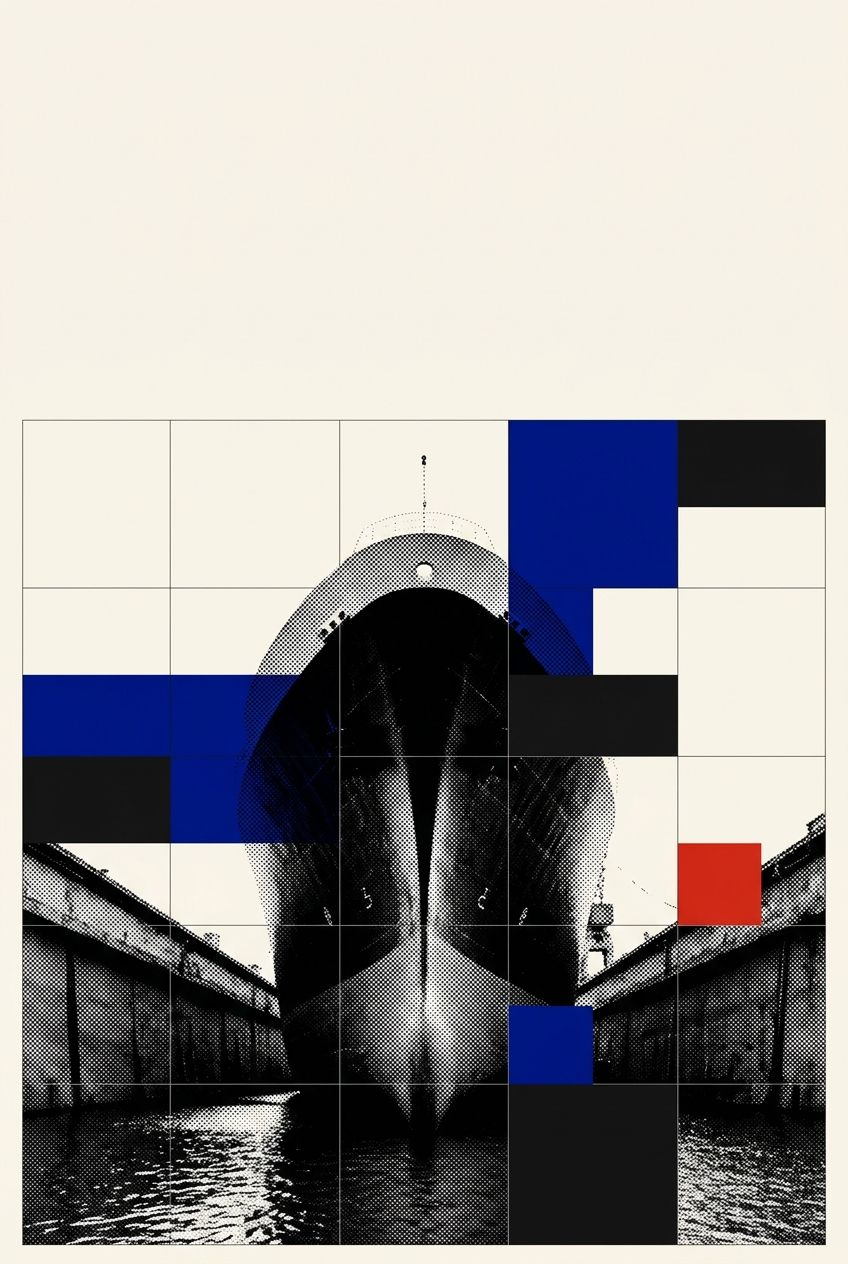
\includegraphics[width=\paperwidth,height=\paperheight]{plates/swiss/cover.jpg}}}}{%
    \PackageError{pd-swiss-plates}{Missing plate render plates/swiss/cover.jpg}{Generate the Swiss cover render and place it at plates/swiss/cover.jpg before building.}}}
\newcommand{\pdswisspartplate}[2]{% #1 numeral I..IV, #2 width
  \IfFileExists{plates/swiss/part-#1.jpg}{%
    \includegraphics[width=#2]{plates/swiss/part-#1.jpg}}{%
    \PackageError{pd-swiss-plates}{Missing plate render plates/swiss/part-#1.jpg}{Generate the Swiss part plate render and place it at plates/swiss/part-#1.jpg before building.}}}
\newcommand{\pdswissplate}[2]{% #1 chapter prefix, #2 width
  \IfFileExists{plates/swiss/chapter-#1.jpg}{%
    \includegraphics[width=#2]{plates/swiss/chapter-#1.jpg}%
  }{%
    \PackageError{pd-swiss-plates}{Missing plate render plates/swiss/chapter-#1.jpg}{Generate the Swiss chapter plate render and place it at plates/swiss/chapter-#1.jpg before building.}%
  }%
}
\newcommand{\pdswissfigplate}[2]{% #1 figure name, #2 width
  \IfFileExists{plates/swiss/#1.jpg}{%
    \includegraphics[width=#2]{plates/swiss/#1.jpg}%
  }{%
    \PackageError{pd-swiss-plates}{Missing figure plate render plates/swiss/#1.jpg}{Generate the Swiss figure plate render and place it at plates/swiss/#1.jpg before building.}%
  }%
}
\providecolor{pdswissred}{HTML}{DA291C}
\providecolor{pdcobalt}{HTML}{001489}
\providecolor{hhink}{HTML}{1B1712}
\providecolor{hhgray}{HTML}{5C5650}

% Canonical Landmark titles and pull-quotes
\expandafter\def\csname pdlandmarktitle@01\endcsname{The Substrate Bedrock \& The Kernel Gap}
\expandafter\def\csname pdlandmarkconcept@01\endcsname{Substrate Bedrock \& The Operating Kernel Gap}
\expandafter\def\csname pdlandmarkquestion@01\endcsname{Which effects require mediation, and which records must survive a failure?}
\expandafter\def\csname pdlandmarkquote@01\endcsname{A proposed action is not evidence that it occurred. A state-dependent admission rule needs adequate evidence of the state on which it depends. When recovery depends on a past event, an adequate record must survive the failure being considered.}

\expandafter\def\csname pdlandmarktitle@02\endcsname{Agentic Continuity \& The Overlapping Strand}
\expandafter\def\csname pdlandmarkconcept@02\endcsname{Substrate Continuity \& Overlapping Strands}
\expandafter\def\csname pdlandmarkquestion@02\endcsname{What makes an obligation survive a change of worker?}
\expandafter\def\csname pdlandmarkquote@02\endcsname{Continuity belongs to a maintained record of authority, obligations and evidence. Processes and models may change while that record persists. A succession rule must identify who inherits each obligation; similarity of behavior alone does not establish accountable identity.}

\expandafter\def\csname pdlandmarktitle@03\endcsname{The Engine Swap}
\expandafter\def\csname pdlandmarkconcept@03\endcsname{The Engine Swap \& Model Portability}
\expandafter\def\csname pdlandmarkquestion@03\endcsname{What must be checked before a replacement model continues the work?}
\expandafter\def\csname pdlandmarkquote@03\endcsname{A model can be replaced without discarding the work record. Safe continuation still requires compatible tools, retained obligations and checks on the replacement worker. Preserving a contract does not establish that the new model can fulfill it.}

\expandafter\def\csname pdlandmarktitle@04\endcsname{The Front-Loaded Probation Cliff}
\expandafter\def\csname pdlandmarkconcept@04\endcsname{The Front-Loaded Probation Cliff}
\expandafter\def\csname pdlandmarkquestion@04\endcsname{What does probation establish, and what risk remains?}
\expandafter\def\csname pdlandmarkquote@04\endcsname{Probation limits exposure while evidence accumulates. Admission depends on an explicit rule, the quality of the evidence and the cost of a mistake. A successful history can justify a bounded grant; it cannot prove that future behavior will be harmless.}

\expandafter\def\csname pdlandmarktitle@05\endcsname{The Single-Writer Monotonic Horizon}
\expandafter\def\csname pdlandmarkconcept@05\endcsname{The Single-Writer Monotonic Horizon}
\expandafter\def\csname pdlandmarkquestion@05\endcsname{What does a local commit order settle, and what lies outside it?}
\expandafter\def\csname pdlandmarkquote@05\endcsname{Within its mediated domain, a serializing writer can give admitted transactions a common commit order. Durability depends on the storage and failure model. That local order does not by itself resolve disagreement between independent operators or prevent effects outside the writer.}

\expandafter\def\csname pdlandmarktitle@06\endcsname{The Attenuation Frontier \& Cryptographic Macaroons}
\expandafter\def\csname pdlandmarkconcept@06\endcsname{The Attenuation Frontier \& Macaroons}
\expandafter\def\csname pdlandmarkquestion@06\endcsname{When does delegation actually narrow authority?}
\expandafter\def\csname pdlandmarkquote@06\endcsname{An attenuated credential adds restrictions to an existing grant. Authority narrows only when the verifier checks the complete delegation chain and enforces every applicable restriction. Possessing a signed credential is not sufficient authorization for an arbitrary action.}

\expandafter\def\csname pdlandmarktitle@07\endcsname{Attestation Without Revelation (The Sealed Harbor)}
\expandafter\def\csname pdlandmarkconcept@07\endcsname{Attestation Without Revelation (Sealed Harbor)}
\expandafter\def\csname pdlandmarkquestion@07\endcsname{What does attestation establish about a private computation?}
\expandafter\def\csname pdlandmarkquote@07\endcsname{Attestation can identify a measured execution environment under a stated trust model. It does not alone prove that a program is correct or that its outputs reveal no private information. Those claims require separate specifications, enforcement and evidence.}

\expandafter\def\csname pdlandmarktitle@08\endcsname{Read-Poverty \& The Legible Swarm}
\expandafter\def\csname pdlandmarkconcept@08\endcsname{Read-Poverty \& Stigmergic Signaling}
\expandafter\def\csname pdlandmarkquestion@08\endcsname{Which evidence is worth an operator's limited attention?}
\expandafter\def\csname pdlandmarkquote@08\endcsname{An operator has a finite inspection budget. Structured summaries and accessible evidence can reduce the cost of a particular decision. Their value depends on what they preserve and what errors they hide; a shorter message is not automatically a better account.}

\expandafter\def\csname pdlandmarktitle@09\endcsname{Skills as Capital vs.\ Token Labor}
\expandafter\def\csname pdlandmarkconcept@09\endcsname{Skills as Capital vs. Perishable Token Labor}
\expandafter\def\csname pdlandmarkquestion@09\endcsname{When does a reusable tool repay its construction cost?}
\expandafter\def\csname pdlandmarkquote@09\endcsname{A reusable tool trades an initial construction and verification cost for repeated execution. It pays off only when sufficient valid uses recover that cost, including maintenance. Deliberation remains necessary where inputs, requirements or the tool itself are uncertain.}

\expandafter\def\csname pdlandmarktitle@10\endcsname{Bonds, Evidence \& Settlement}
\expandafter\def\csname pdlandmarkconcept@10\endcsname{Bonds, Evidence \& Settlement}
\expandafter\def\csname pdlandmarkquestion@10\endcsname{When can a bond deter a violation that evidence can establish?}
\expandafter\def\csname pdlandmarkquote@10\endcsname{A bond changes incentives only when a violation can be established and the sanction collected. Coverage, detection and deterrence are separate calculations. Settlement must follow the agreed evidence and dispute rules; collateral does not make every harmful action observable.}

\expandafter\def\csname pdlandmarktitle@11\endcsname{Cycle Consistency \& Its Limits}
\expandafter\def\csname pdlandmarkconcept@11\endcsname{Sheaf Laplacians \& Cycle Holonomy}
\expandafter\def\csname pdlandmarkquestion@11\endcsname{Which inconsistencies can cycle checks expose, and which can they miss?}
\expandafter\def\csname pdlandmarkquote@11\endcsname{Cycle checks compare recorded claims under specified observation and restriction maps. A nonzero residual witnesses inconsistency in those records; it does not identify a liar or establish malicious intent. Zero residual also leaves the observation model's blind spots unresolved.}

\expandafter\def\csname pdlandmarktitle@12\endcsname{The Zombie Reclaim \& Salvage Graveyard}
\expandafter\def\csname pdlandmarkconcept@12\endcsname{Zombie Salvage \& Dead-Man Leases}
\expandafter\def\csname pdlandmarkquestion@12\endcsname{How can work be reassigned without admitting a stale worker?}
\expandafter\def\csname pdlandmarkquote@12\endcsname{A missing heartbeat is evidence of silence, not proof of death. Reassignment requires an expiry rule, retained work state and fencing that rejects a stale holder's writes to the reassigned resource. Recovery must also account for effects whose completion was never recorded.}

% Single-digit alias fallbacks
\expandafter\def\csname pdlandmarktitle@1\endcsname{\csname pdlandmarktitle@01\endcsname}
\expandafter\def\csname pdlandmarkconcept@1\endcsname{\csname pdlandmarkconcept@01\endcsname}
\expandafter\def\csname pdlandmarkquestion@1\endcsname{\csname pdlandmarkquestion@01\endcsname}
\expandafter\def\csname pdlandmarkquote@1\endcsname{\csname pdlandmarkquote@01\endcsname}

\expandafter\def\csname pdlandmarktitle@2\endcsname{\csname pdlandmarktitle@02\endcsname}
\expandafter\def\csname pdlandmarkconcept@2\endcsname{\csname pdlandmarkconcept@02\endcsname}
\expandafter\def\csname pdlandmarkquestion@2\endcsname{\csname pdlandmarkquestion@02\endcsname}
\expandafter\def\csname pdlandmarkquote@2\endcsname{\csname pdlandmarkquote@02\endcsname}

\expandafter\def\csname pdlandmarktitle@3\endcsname{\csname pdlandmarktitle@03\endcsname}
\expandafter\def\csname pdlandmarkconcept@3\endcsname{\csname pdlandmarkconcept@03\endcsname}
\expandafter\def\csname pdlandmarkquestion@3\endcsname{\csname pdlandmarkquestion@03\endcsname}
\expandafter\def\csname pdlandmarkquote@3\endcsname{\csname pdlandmarkquote@03\endcsname}

\expandafter\def\csname pdlandmarktitle@4\endcsname{\csname pdlandmarktitle@04\endcsname}
\expandafter\def\csname pdlandmarkconcept@4\endcsname{\csname pdlandmarkconcept@04\endcsname}
\expandafter\def\csname pdlandmarkquestion@4\endcsname{\csname pdlandmarkquestion@04\endcsname}
\expandafter\def\csname pdlandmarkquote@4\endcsname{\csname pdlandmarkquote@04\endcsname}

\expandafter\def\csname pdlandmarktitle@5\endcsname{\csname pdlandmarktitle@05\endcsname}
\expandafter\def\csname pdlandmarkconcept@5\endcsname{\csname pdlandmarkconcept@05\endcsname}
\expandafter\def\csname pdlandmarkquestion@5\endcsname{\csname pdlandmarkquestion@05\endcsname}
\expandafter\def\csname pdlandmarkquote@5\endcsname{\csname pdlandmarkquote@05\endcsname}

\expandafter\def\csname pdlandmarktitle@6\endcsname{\csname pdlandmarktitle@06\endcsname}
\expandafter\def\csname pdlandmarkconcept@6\endcsname{\csname pdlandmarkconcept@06\endcsname}
\expandafter\def\csname pdlandmarkquestion@6\endcsname{\csname pdlandmarkquestion@06\endcsname}
\expandafter\def\csname pdlandmarkquote@6\endcsname{\csname pdlandmarkquote@06\endcsname}

\expandafter\def\csname pdlandmarktitle@7\endcsname{\csname pdlandmarktitle@07\endcsname}
\expandafter\def\csname pdlandmarkconcept@7\endcsname{\csname pdlandmarkconcept@07\endcsname}
\expandafter\def\csname pdlandmarkquestion@7\endcsname{\csname pdlandmarkquestion@07\endcsname}
\expandafter\def\csname pdlandmarkquote@7\endcsname{\csname pdlandmarkquote@07\endcsname}

\expandafter\def\csname pdlandmarktitle@8\endcsname{\csname pdlandmarktitle@08\endcsname}
\expandafter\def\csname pdlandmarkconcept@8\endcsname{\csname pdlandmarkconcept@08\endcsname}
\expandafter\def\csname pdlandmarkquestion@8\endcsname{\csname pdlandmarkquestion@08\endcsname}
\expandafter\def\csname pdlandmarkquote@8\endcsname{\csname pdlandmarkquote@08\endcsname}

\expandafter\def\csname pdlandmarktitle@9\endcsname{\csname pdlandmarktitle@09\endcsname}
\expandafter\def\csname pdlandmarkconcept@9\endcsname{\csname pdlandmarkconcept@09\endcsname}
\expandafter\def\csname pdlandmarkquestion@9\endcsname{\csname pdlandmarkquestion@09\endcsname}
\expandafter\def\csname pdlandmarkquote@9\endcsname{\csname pdlandmarkquote@09\endcsname}

\newcommand{\pdswisslandmarkplate}[2]{% #1 landmark ID (e.g. 01..12), #2 width
  \IfFileExists{plates/swiss/landmark-#1.jpg}{%
    \centering
    \includegraphics[width=#2]{plates/swiss/landmark-#1.jpg}%
    \par\vspace{10pt}%
    \begin{minipage}{\linewidth}%
      {\color{pdcobalt}\rule{\linewidth}{1.2pt}}\par\vspace{6pt}%
      \raggedright
      {\color{pdswissred}\rule{4.5pt}{4.5pt}}\enspace%
      {\pdgrotesk\bfseries\scshape\fontsize{9}{11}\selectfont\color{hhink}%
        Landmark #1\enspace\textperiodcentered\enspace\csname pdlandmarktitle@#1\endcsname}\par\vspace{4.5pt}%
      {\pdgrotesk\itshape\fontsize{9.5}{13.5}\selectfont\color{hhink}%
        \csname pdlandmarkquote@#1\endcsname\par}%
      \vspace{6pt}%
      {\color{hhgray!30}\rule{\linewidth}{0.4pt}}%
    \end{minipage}%
  }{%
    \PackageError{pd-swiss-plates}{Missing plate render plates/swiss/landmark-#1.jpg}{Generate the Swiss landmark plate render and place it at plates/swiss/landmark-#1.jpg before building.}}}
\makeatother

\fi
% Wordless interstitial art for the Swiss Book, not numbered evidence figures.
% Insert only at an authored paragraph boundary. On verso the plate faces
% following text; on recto it faces preceding text. Never split an arbitrary
% text page, paragraph, worked example, or proof to manufacture verso parity.
\makeatletter
\providecommand{\pdreflectionrecord}[2]{}
\providecommand*{\toclevel@pdplate}{1}
\definecolor{pdreflectionpanel}{HTML}{00564C}
% Interstitials have their own contents entry; they must not advance the
% chapter-art counter used by the illustrated chapter contents.
\newcommand{\pdreflectiontitle}[2]{%
  \expandafter\def\csname pd@reflection@title@#1\endcsname{#2}}
\pdreflectiontitle{the-unseen-boat}{What a summary leaves unseen}
\pdreflectiontitle{the-waiting-body}{What survives the worker}
\pdreflectiontitle{the-paper-crossing}{A commitment between independent shores}
\pdreflectiontitle{the-controlled-opening}{The controlled opening}
% Text-bearing plates declare their own reserved, opaque lower panel.
% Existing wordless plates do not acquire generic captions or title bars.
\newcommand{\pdreflectionbody}[2]{%
  \expandafter\def\csname pd@reflection@body@#1\endcsname{#2}}
\pdreflectionbody{the-controlled-opening}{%
  A closed cabinet still has a slot. A confined agent still has an output.
  The noninterference claim must name what that output may reveal and which
  other channels the model excludes.}
\newcommand{\pdreflectiontocentry}[2]{%
  \begin{minipage}[c]{.19\linewidth}%
    \includegraphics[width=\linewidth,height=.62in,keepaspectratio]{plates/interstitial/#1.jpg}%
  \end{minipage}\hfill
  \begin{minipage}[c]{.76\linewidth}\raggedright\small
    Plate: #2%
  \end{minipage}}
\newcommand*{\l@pdplate}[2]{%
  \par\addvspace{7pt}\noindent
  \begin{minipage}[c]{.90\linewidth}#1\end{minipage}\hfill
  \makebox[.07\linewidth][r]{\small #2}\par\addvspace{7pt}}
\newcommand{\pd@reflection@render}[1]{%
  \IfFileExists{plates/interstitial/#1.jpg}{%
    \thispagestyle{empty}%
    \ifcsname pd@reflection@title@#1\endcsname
      \phantomsection\label{plate:#1}%
      \addcontentsline{toc}{pdplate}{\protect\texorpdfstring{\protect\pdreflectiontocentry{#1}{\csname pd@reflection@title@#1\endcsname}}{Plate: \csname pd@reflection@title@#1\endcsname}}%
    \else
      \PackageError{pd-reflection-plates}{Missing contents title for #1}%
        {Register this plate with pdreflectiontitle before placing it.}%
    \fi
    \protected@write\@auxout{}{\string\pdreflectionrecord{#1}{\thepage}}%
    \AddToShipoutPictureBG*{\AtPageCenter{\makebox(0,0){%
      \includegraphics[width=6in,height=9in,keepaspectratio]{plates/interstitial/#1.jpg}}}}%
    \ifcsname pd@reflection@body@#1\endcsname
      \AddToShipoutPictureFG*{\AtPageCenter{\makebox(0,0){\begingroup
        % Page art is not a column figure. Undo the Book's centering wrapper,
        % as the existing full-page cover renderer does.
        \ifdefined\pd@typesetpicturebox\let\pgfsys@typesetpicturebox\pd@typesetpicturebox\fi
        \begin{tikzpicture}[x=1in,y=1in]
          \useasboundingbox (0,0) rectangle (6,9);
          \fill[pdreflectionpanel] (0,0) rectangle (6,2.45);
          \node[anchor=north west,inner sep=0,text=white,text width=5in,
            font=\fontsize{17}{21}\selectfont\bfseries] at (.5,2.05)
            {\csname pd@reflection@title@#1\endcsname};
          \node[anchor=north west,inner sep=0,text=white,text width=5in,
            font=\fontsize{11}{15}\selectfont,align=left] at (.5,1.5)
            {\raggedright\hyphenpenalty=10000\csname pd@reflection@body@#1\endcsname};
        \end{tikzpicture}\endgroup}}}%
    \fi
    \null\newpage
  }{\PackageError{pd-reflection-plates}{Missing interstitial plate #1}%
    {Restore plates/interstitial/#1.jpg and its provenance before building.}}%
}
\newcommand{\pd@reflection@place}[1]{%
  \clearpage
  \pd@reflection@render{#1}%
}
\newcommand{\pdreflectionplate}[1]{%
  \ifpdswiss\pd@reflection@place{#1}\fi
}
\makeatother

\newif\ifpdcopyreview
\pdcopyreviewfalse
% coordination-papers-mega-volume-epigraph-review-spreads.tex
% Editorial 2-page review spreads presenting incumbent and contender epigraphs
% immediately preceding each chapter opener plate page (Chapters 0 through 8).
% Every spread clearly marks header and footer:
% "COPY REVIEW NOTES ONLY, NOT FOR PUBLICATION"

\makeatletter

% ---------------------------------------------------------------------------
% Page Style for Copy Review Spreads
% ---------------------------------------------------------------------------
\newcommand{\pdreviewchapnum}{0}

\fancypagestyle{pdcopyreview}{%
  \fancyhf{}%
  \fancyhfoffset[LE,RO]{0.9in}%
  \fancyhead[C]{\small\bfseries\color{pderror}\textsf{COPY REVIEW NOTES ONLY, NOT FOR PUBLICATION}}%
  \fancyhead[LE,RO]{\small\sffamily\bfseries\color{hhgray}\thepage}%
  \fancyhead[RE,LO]{}%
  \fancyfoot[C]{\small\bfseries\color{pderror}\textsf{COPY REVIEW NOTES ONLY, NOT FOR PUBLICATION}}%
  \fancyfoot[LE,RO]{\small\sffamily\bfseries\color{hhgray}\thepage}%
  \fancyfoot[RE,LO]{}%
  \renewcommand{\headrulewidth}{0.5pt}%
  \renewcommand{\footrulewidth}{0.5pt}%
  \renewcommand{\headrule}{\hbox to\headwidth{\color{pderror}\leaders\hrule height \headrulewidth\hfill}}%
  \renewcommand{\footrule}{\hbox to\headwidth{\color{pderror}\leaders\hrule height \footrulewidth\hfill}}%
}

% ---------------------------------------------------------------------------
% Spread Layout Building Blocks
% ---------------------------------------------------------------------------
\newcommand{\pdreviewheader}[5]{%
  \renewcommand{\pdreviewchapnum}{#1}%
  \noindent{\pdgrotesk\footnotesize\bfseries\color{pderror}\textsc{Copy Review Notes \textbullet\ Alternative Epigraphs Dossier}}\hfill{\pdgrotesk\footnotesize\color{hhgray}Facing Verso / Page 1 of 2}\par
  \vspace{4pt}
  \noindent{\pddisplayface\LARGE\bfseries Chapter #1: #2\par}
  \vspace{2pt}
  \noindent{\pdgrotesk\small\bfseries\color{#5}Theme: #3\par}
  \vspace{1pt}
  \noindent{\pdgrotesk\footnotesize\color{hhgray}Core Question: \emph{#4}}\par
  \vspace{3pt}\noindent{\color{#5}\rule{\linewidth}{1.2pt}}\par
  \vspace{5pt}
}

\newcommand{\pdreviewboxincumbent}[5]{%
  \begin{tcolorbox}[colback=hhpaper,colframe=#5,arc=2pt,boxrule=0.8pt,top=5pt,bottom=5pt,left=7pt,right=7pt]
  {\pdgrotesk\footnotesize\bfseries\color{#5}\textsc{Incumbent Epigraph \textbullet\ Currently Bound in Volume}}\hfill{\pdgrotesk\scriptsize\color{hhgray}Word Count: #3 words}\par\vspace{3pt}
  \noindent{\normalsize\itshape ``#1''}
  \par\vspace{3pt}
  \noindent\hfill{\pdgrotesk\footnotesize\bfseries --- #2}\par\vspace{4pt}
  \noindent{\pdgrotesk\scriptsize\bfseries\color{hhgray}EDITORIAL VERDICT:}\par
  {\pdgrotesk\footnotesize #4\par}
  \end{tcolorbox}
}

\newcommand{\pdreviewboxcontender}[5]{%
  \begin{tcolorbox}[colback=hhpaper,colframe=hhgray!50,arc=2pt,boxrule=0.6pt,top=5pt,bottom=5pt,left=7pt,right=7pt]
  {\pdgrotesk\footnotesize\bfseries\color{hhink}\textsc{Contender #1 \textbullet\ Alternative Option}}\hfill{\pdgrotesk\scriptsize\color{hhgray}Word Count: #4 words}\par\vspace{3pt}
  \noindent{\normalsize\itshape ``#2''}
  \par\vspace{3pt}
  \noindent\hfill{\pdgrotesk\footnotesize\bfseries --- #3}\par\vspace{4pt}
  \noindent{\pdgrotesk\scriptsize\bfseries\color{hhgray}SYSTEMS \& ECONOMIC RESONANCE:}\par
  {\pdgrotesk\footnotesize #5\par}
  \end{tcolorbox}
}

\newcommand{\pdreviewboxrubric}[2]{%
  \begin{tcolorbox}[colback=hhpaper,colframe=pderror!70,arc=2pt,boxrule=0.6pt,top=5pt,bottom=5pt,left=7pt,right=7pt]
  {\pdgrotesk\footnotesize\bfseries\color{pderror}\textsc{Editorial Synthesis \textbullet\ Reviewer Decision Rubric}}\par\vspace{3pt}
  {\pdgrotesk\footnotesize
  \textbf{Recommendation:} #1\par\vspace{3pt}
  \textbf{Backup Choice:} #2\par}
  \end{tcolorbox}
}

% ---------------------------------------------------------------------------
% Chapter 0 Spread
% ---------------------------------------------------------------------------
\def\pdepigraphreviewspread@zero{%
  % Page 1 (Verso)
  \begin{adjustwidth*}{0pt}{-0.9in}
  \pdreviewheader{0}{Foundations and Prerequisites}{Classical Multi-Agent Theory, Modern LLM Physics, and the Kernel Gap}{What physical and theoretical ground must an agent operating kernel stand on?}{pdslate}
  \pdreviewboxincumbent{There are two ways of constructing a software design: One way is to make it so simple that there are obviously no deficiencies, and the other way is to make it so complicated that there are no obvious deficiencies. The first method is far more difficult.}{C.\,A.\,R. Hoare, \emph{The Emperor's Old Clothes} (1980 Turing Award Lecture)}{38}{Sets up the core thesis of Chapter 0: autonomous swarms relying on prompt cajoling create architectures so complicated there are no obvious deficiencies until production fails. A formal single-writer kernel achieves the first, more difficult method: obvious simplicity.}{pdslate}
  \vspace{6pt}
  \pdreviewboxcontender{A}{The hard problems are ancient; the easy problems are new.}{Hans Moravec, \emph{Mind Children: The Future of Robot and Human Intelligence} (1988), Chapter 1, p.\ 15}{10}{The canonical statement of Moravec's Paradox. Fluent syntactic generation is new and easy; memory durability, process continuity, and physical synchronization are ancient and difficult. Striking and pithy, but previously overused across earlier drafts.}
  \vfill
  \end{adjustwidth*}
  \clearpage
  % Page 2 (Recto)
  \begin{adjustwidth*}{0pt}{-0.9in}
  \pdreviewboxcontender{B}{The Analytical Engine has no pretensions whatever to originate any thing. It can do whatever we know how to order it to perform.}{Ada Lovelace, \emph{Notes upon the Memoir by L. F. Menabrea} (1843), Note G}{23}{The ultimate foundational observation on algorithmic computation. Autoregressive language models do not originate volition or intentionality; they sample token distributions. Real agentic governance requires an external operating system to order and constrain execution.}
  \vspace{6pt}
  \pdreviewboxcontender{C}{The competent programmer is fully aware of the strictly limited size of his own skull; therefore he approaches the programming task in full humility, and among other things he avoids clever tricks like the plague.}{Edsger W. Dijkstra, \emph{The Humble Programmer} (1972 Turing Award Lecture)}{33}{Dijkstra's rebuke to ungrounded complexity directly targets the fragility of multi-agent prompt chains. Swarms fail when developers substitute clever prompt tricks for humble, verifiable kernel primitives.}
  \vspace{6pt}
  \pdreviewboxrubric{Retain \textbf{C.\,A.\,R. Hoare (1980)} as the canonical Chapter 0 epigraph. It frames the entire book's technical contrast between brittle prompt engineering (``no obvious deficiencies'') and mathematical kernel invariants (``obviously no deficiencies'').}{Retain \textbf{Ada Lovelace (1843)} as backup if philosophical demarcation between generative fluency and mechanical agency is preferred.}
  \vfill
  \end{adjustwidth*}
  \clearpage
}

% ---------------------------------------------------------------------------
% Chapter 1 Spread
% ---------------------------------------------------------------------------
\def\pdepigraphreviewspread@one{%
  % Page 1 (Verso)
  \begin{adjustwidth*}{0pt}{-0.9in}
  \pdreviewheader{1}{The Single-Writer Kernel}{SQLite WAL, Serial Mutation, Crash Durability, and the Single-Writer Horizon}{Where can a rule be made real?}{pdcobalt}
  \pdreviewboxincumbent{There is no fundamental need to keep a database at all; the log is all the information there is. The only reason for storing the database is performance of retrieval operations.}{Jim Gray and Andreas Reuter, \emph{Transaction Processing: Concepts and Techniques} (1993), Section 10.1, p.\ 493}{29}{Jim Gray (1998 Turing Award winner and father of ACID/WAL) provides the architectural manifesto for Chapter 1: the write-ahead log is the ultimate reality; database tables and indexes are mere disposable projections.}{pdcobalt}
  \vspace{6pt}
  \pdreviewboxcontender{A}{Log updates to record the truth about the state of an object\dots\ Since the log is append-only, it is easy to write reliably to stable storage that survives a crash.}{Butler W. Lampson, ``Hints for Computer System Design'', \emph{ACM Operating Systems Review}, SOSP '83 (1983), Section 3.3, p.\ 39}{28}{Lampson's classic hint crystallizes the transition from volatile in-memory claims to durable local truth. It strips away academic hand-waving and identifies stable, sequential disk writes as the bedrock of fault tolerance.}
  \vfill
  \end{adjustwidth*}
  \clearpage
  % Page 2 (Recto)
  \begin{adjustwidth*}{0pt}{-0.9in}
  \pdreviewboxcontender{B}{A distributed system is one in which the failure of a computer you didn't even know existed can render your own computer unusable.}{Leslie Lamport, message to a DEC SRC bulletin board, 28 May 1987}{21}{The universally recognized definition of distributed dread. Chapter 1 deliberately avoids multi-machine consensus protocols by grounding serialization in a local, crash-proof single-writer disk log.}
  \vspace{6pt}
  \pdreviewboxcontender{C}{Covenants, without the sword, are but words and of no strength to secure a man at all.}{Thomas Hobbes, \emph{Leviathan: Or the Matter, Forme and Power of a Commonwealth} (1651), Part II, Chapter XVII, p.\ 85}{18}{A political philosophy parallel that answers the chapter question with razor precision: coordination protocols and contracts are meaningless without an enforcement mechanism. The local durable disk is the sword that gives weight to the rule.}
  \vspace{6pt}
  \pdreviewboxrubric{Retain \textbf{Jim Gray \& Andreas Reuter (1993)}. It defines the physical primacy of the write-ahead log as ground truth.}{Retain \textbf{Butler Lampson (1983)} for systems-design perspective; \textbf{Leslie Lamport (1987)} if humorous cynicism regarding distributed consensus is desired.}
  \vfill
  \end{adjustwidth*}
  \clearpage
}

% ---------------------------------------------------------------------------
% Chapter 2 Spread
% ---------------------------------------------------------------------------
\def\pdepigraphreviewspread@two{%
  % Page 1 (Verso)
  \begin{adjustwidth*}{0pt}{-0.9in}
  \pdreviewheader{2}{The Anchor Protocol}{Attenuation Frontier, Least Privilege, Cryptographic Capabilities, and Macaroons}{How may authority travel without silently growing?}{pdcobalt}
  \pdreviewboxincumbent{Every program and every user of the system should operate using the least set of privileges necessary to complete the job.}{Jerome H. Saltzer and Michael D. Schroeder, \emph{The Protection of Information in Computer Systems}, Proceedings of the IEEE (1975), Section 1.4, p.\ 1282}{17}{The canonical, historical definition of the Principle of Least Privilege (PoLP). Authoritative and historically unassailable, though describes administrative policy rather than dynamic cryptographic delegation.}{pdcobalt}
  \vspace{6pt}
  \pdreviewboxcontender{A}{Target services can verify credentials without communicating with the issuing service, and clients can freely attenuate credentials by adding caveats.}{Arnar Birgisson et al., ``Macaroons: Cookies with Contextual Caveats for Decentralized Authorization in the Cloud'', \emph{NDSS '14} (2014), Section 1, p.\ 1}{19}{The exact technical mechanism of the Anchor Protocol. Authority travels without phone-home verification, and each intermediary can only monotonically reduce (attenuate) rights by chaining cryptographic caveats.}
  \vfill
  \end{adjustwidth*}
  \clearpage
  % Page 2 (Recto)
  \begin{adjustwidth*}{0pt}{-0.9in}
  \pdreviewboxcontender{B}{A capability is an unforgeable ticket, which when presented can be taken as incontestable proof that the presenter is authorized to have access to the object.}{Butler W. Lampson, ``Protection'', \emph{ACM Operating Systems Review}, Vol.\ 8, No.\ 1 (1974), Section 1, p.\ 20}{26}{Lampson's definition of an object capability replaces ambient authority and identity lookups with bearer tickets, establishing the formal baseline for unforgeable delegated rights.}
  \vspace{6pt}
  \pdreviewboxcontender{C}{Constant experience shows us that every man invested with power is apt to abuse it, and to carry his authority as far as it will go.}{Montesquieu, \emph{The Spirit of the Laws} (1748), Book XI, Chapter 4 (trans.\ Thomas Nugent, 1752)}{26}{Explains why the attenuation frontier must be enforced by mathematics rather than goodwill: authority inherently expands to fill all available space unless structural constraints actively bind it.}
  \vspace{6pt}
  \pdreviewboxrubric{Retain \textbf{Jerome Saltzer \& Michael Schroeder (1975)} for historical bedrock, OR promote \textbf{Arnar Birgisson et al. (2014)} for direct cryptographic mechanism alignment.}{Retain \textbf{Butler Lampson (1974)} for pure object capability semantics.}
  \vfill
  \end{adjustwidth*}
  \clearpage
}

% ---------------------------------------------------------------------------
% Chapter 3 Spread
% ---------------------------------------------------------------------------
\def\pdepigraphreviewspread@three{%
  % Page 1 (Verso)
  \begin{adjustwidth*}{0pt}{-0.9in}
  \pdreviewheader{3}{The Sealed Harbor}{Sandbox Confinement, Information Flow Lattices, and Leakage Budgets}{What can a sealed agent leak, and how would we know?}{pdteal}
  \pdreviewboxincumbent{The problem is to confine an arbitrary program, which may have been written by someone else, so that it cannot transmit information to any other program except its caller.}{Butler W. Lampson, ``A Note on the Confinement Problem'', \emph{Communications of the ACM}, Vol.\ 16, No.\ 10 (1973), Section 1, p.\ 613}{27}{The landmark paper that formally introduced the ``confinement problem'' and ``covert channels'' to computer science. Describes the sealed harbor verbatim: executing untrusted third-party code where every egress path is bounded and observed.}{pdteal}
  \vspace{6pt}
  \pdreviewboxcontender{A}{Information flow from storage class A to storage class B is permissible only if the flow relation holds: $A \le B$.}{Dorothy E. Denning, ``A Lattice Model of Secure Information Flow'', \emph{Communications of the ACM}, Vol.\ 19, No.\ 5 (1976), Section 2, p.\ 238}{21}{Provides the formal information-flow lattice underlying secure isolation. It models leakage not as good intentions, but as an invariant over ordered security classes.}
  \vfill
  \end{adjustwidth*}
  \clearpage
  % Page 2 (Recto)
  \begin{adjustwidth*}{0pt}{-0.9in}
  \pdreviewboxcontender{B}{Any logically irreversible manipulation of information, such as the erasure of a bit or the merging of two computation paths, must be accompanied by a corresponding entropy increase.}{Rolf Landauer, ``Irreversibility and Heat Generation in the Computing Process'', \emph{IBM Journal of Research and Development} (1961), Section 1, p.\ 183}{27}{Reflects the chapter's core physical insight: ``the budget of what can leak is a ledger that conserves.'' Compute leaves observable thermodynamic entropy across physical boundaries.}
  \vspace{6pt}
  \pdreviewboxcontender{C}{Whereof one cannot speak, thereof one must be silent.}{Ludwig Wittgenstein, \emph{Tractatus Logico-Philosophicus}, proposition 7 (1921), trans.\ C.\,K. Ogden (1922)}{8}{Poetic and evocative of complete isolation, though philosophically about the limits of language rather than covert microarchitectural side channels.}
  \vspace{6pt}
  \pdreviewboxrubric{Retain \textbf{Butler W. Lampson (1973)}. It is the canonical foundation of confinement in operating systems.}{Retain \textbf{Dorothy Denning (1976)} for information lattice flow precision; \textbf{Rolf Landauer (1961)} for physical conservation laws.}
  \vfill
  \end{adjustwidth*}
  \clearpage
}

% ---------------------------------------------------------------------------
% Chapter 4 Spread
% ---------------------------------------------------------------------------
\def\pdepigraphreviewspread@four{%
  % Page 1 (Verso)
  \begin{adjustwidth*}{0pt}{-0.9in}
  \pdreviewheader{4}{The Legible Swarm}{Read-Poverty, Stigmergy, Cognitive Load, and Human Attention Economics}{What must remain visible, and what does seeing cost?}{pdteal}
  \pdreviewboxincumbent{In an information-rich world, the wealth of information means a dearth of something else: a scarcity of whatever it is that information consumes. What information consumes is rather obvious: it consumes the attention of its recipients.}{Herbert A. Simon, ``Designing Organizations for an Information-Rich World'' (1971), pp.\ 40--41}{35}{The definitive formulation of attention economics by Nobel laureate Herbert Simon. An autonomous swarm generates limitless telemetry; the scarce resource is never log volume, but the operator's attention.}{pdteal}
  \vspace{6pt}
  \pdreviewboxcontender{A}{Certain forms of knowledge and control require a narrowing of vision. The great advantage of such tunnel vision is that it brings into sharp focus certain limited aspects of an otherwise far more complex and unwieldy reality.}{James C. Scott, \emph{Seeing Like a State} (1998), Introduction, p.\ 11}{36}{Scott's concept of ``legibility'' inspired the chapter title and explains how administrative abstractions simplify complex realities at the risk of losing tacit local context.}
  \vfill
  \end{adjustwidth*}
  \clearpage
  % Page 2 (Recto)
  \begin{adjustwidth*}{0pt}{-0.9in}
  \pdreviewboxcontender{B}{The capacity of any regulator is limited by its capacity as a channel of communication.}{W. Ross Ashby, \emph{An Introduction to Cybernetics} (1956), Chapter 11, Section 13, p.\ 211}{15}{Origin of the Law of Requisite Variety. An operator cannot govern or regulate an autonomous fleet whose variety exceeds the supervisory channel capacity.}
  \vspace{6pt}
  \pdreviewboxcontender{C}{The fundamental problem of communication is that of reproducing at one point either exactly or approximately a message selected at another point.}{Claude E. Shannon, ``A Mathematical Theory of Communication'', \emph{Bell System Technical Journal} (1948), Section 1, p.\ 379}{21}{Prices supervision directly in bits. Summaries that discard raw entropy without verifiable links back to primary evidence create catastrophic operator blindness.}
  \vspace{6pt}
  \pdreviewboxrubric{Retain \textbf{Herbert A. Simon (1971)}. Attention economics is the exact problem of swarm telemetry.}{Retain \textbf{James C. Scott (1998)} for organizational legibility; \textbf{W. Ross Ashby (1956)} for cybernetic regulator limits.}
  \vfill
  \end{adjustwidth*}
  \clearpage
}

% ---------------------------------------------------------------------------
% Chapter 5 Spread
% ---------------------------------------------------------------------------
\def\pdepigraphreviewspread@five{%
  % Page 1 (Verso)
  \begin{adjustwidth*}{0pt}{-0.9in}
  \pdreviewheader{5}{From Spawn to Person}{Identity Continuity, Episodic Memory, Forensic Personhood, and Accountability Across Restarts}{What remains long enough to owe anything?}{pdamber}
  \pdreviewboxincumbent{We are but whirlpools in a river of ever-flowing water. We are not stuff that abides, but patterns that perpetuate themselves.}{Norbert Wiener, \emph{The Human Use of Human Beings: Cybernetics and Society} (1950), Chapter 5, p.\ 96}{21}{Norbert Wiener captures the essence of agentic continuity: processes, threads, and tokens are ephemeral, but identity is an informational pattern that perpetuates across restarts.}{pdamber}
  \vspace{6pt}
  \pdreviewboxcontender{A}{Person, as I take it, is the name for this self. It is a forensic term, appropriating actions and their merit; and so belongs only to intelligent agents, capable of a law, and happiness, and misery.}{John Locke, \emph{An Essay Concerning Human Understanding} (1690), Book II, Chapter xxvii, Section 26}{33}{A monumental philosophical definition. Locke identifies personhood not as biological substance, but as a forensic accounting construct that appropriates actions and responsibility over time.}
  \vfill
  \end{adjustwidth*}
  \clearpage
  % Page 2 (Recto)
  \begin{adjustwidth*}{0pt}{-0.9in}
  \pdreviewboxcontender{B}{To breed an animal with the right to make promises---is not this the paradoxical task that nature has set itself with regard to man?}{Friedrich Nietzsche, \emph{On the Genealogy of Morals} (1887), Second Essay, Section 1 (trans.\ Walter Kaufmann)}{22}{Electrifying resonance with the chapter's core dilemma: turning ephemeral processes into durable entities capable of binding themselves to future commitments and contracts.}
  \vspace{6pt}
  \pdreviewboxcontender{C}{A person is not a separately existing entity, distinct from his experiences\dots\ What matters is psychological continuity and connectedness.}{Derek Parfit, \emph{Reasons and Persons} (1984), Part 3, Chapter 12, p.\ 215}{19}{Demystifies identity. Personal identity is not a mystical soul, but overlapping chains of cause, memory, and intention---the exact role of append-only event logs in agent systems.}
  \vspace{6pt}
  \pdreviewboxrubric{Retain \textbf{Norbert Wiener (1950)}. It speaks directly to cybernetic patterns surviving physical resets.}{Retain \textbf{John Locke (1690)} for forensic accountability; \textbf{Friedrich Nietzsche (1887)} for binding promises.}
  \vfill
  \end{adjustwidth*}
  \clearpage
}

% ---------------------------------------------------------------------------
% Chapter 6 Spread
% ---------------------------------------------------------------------------
\def\pdepigraphreviewspread@six{%
  % Page 1 (Verso)
  \begin{adjustwidth*}{0pt}{-0.9in}
  \pdreviewheader{6}{The Harbor Economy}{Labor vs Capital, Token Economics, Asset Rental, and Conservation Laws}{What makes cooperation rational without making loss unbounded?}{pdamber}
  \pdreviewboxincumbent{The main reason why it is profitable to establish a firm would seem to be that there is a cost of using the price mechanism.}{Ronald H. Coase, ``The Nature of the Firm'', \emph{Economica}, Vol.\ 4, No.\ 16 (1937), Section 2, p.\ 390}{24}{Ronald Coase's Nobel Prize-winning insight explains why harbors exist: market transactions have coordination, contract, and discovery costs. The harbor is an institutional firm for agents.}{pdamber}
  \vspace{6pt}
  \pdreviewboxcontender{A}{Virtually every commercial transaction has within itself an element of trust, certainly any transaction conducted over a period of time.}{Kenneth J. Arrow, ``Gifts and Exchanges'', \emph{Philosophy \& Public Affairs}, Vol.\ 1, No.\ 4 (1972), p.\ 357}{20}{Nobel laureate Kenneth Arrow highlights trust as an invisible economic input. In agent swarms, verifiable cryptographic receipts replace human social trust.}
  \vfill
  \end{adjustwidth*}
  \clearpage
  % Page 2 (Recto)
  \begin{adjustwidth*}{0pt}{-0.9in}
  \pdreviewboxcontender{B}{We must look at the price system as such a mechanism for communicating information if we want to understand its real function.}{Friedrich A. Hayek, ``The Use of Knowledge in Society'', \emph{The American Economic Review}, Vol.\ 35, No.\ 4 (1945), Section VI, p.\ 527}{21}{Prices in an agent economy are compressed information signals that coordinate scarce compute, token allocations, and GPU time across autonomous entities without central control.}
  \vspace{6pt}
  \pdreviewboxcontender{C}{Like all systems involving goals, resources, and actions, computation can be viewed in economic terms.}{Mark S. Miller and K. Eric Drexler, ``Markets and Computation: Agoric Open Systems'' (1988), Section 1, p.\ 133}{15}{The founding paper of agoric computation. It treats processes not as passive code, but as economic actors trading scarce compute and services under conserving budget rules.}
  \vspace{6pt}
  \pdreviewboxrubric{Retain \textbf{Ronald H. Coase (1937)}. It provides the exact theoretical justification for why harbors are organized as institutions rather than pure spot markets.}{Retain \textbf{Mark Miller \& Eric Drexler (1988)} for agoric systems; \textbf{Friedrich Hayek (1945)} for pricing signals.}
  \vfill
  \end{adjustwidth*}
  \clearpage
}

% ---------------------------------------------------------------------------
% Chapter 7 Spread
% ---------------------------------------------------------------------------
\def\pdepigraphreviewspread@seven{%
  % Page 1 (Verso)
  \begin{adjustwidth*}{0pt}{-0.9in}
  \pdreviewheader{7}{The Bonded Commons}{Sacrificial Slashing, Bonded Escrow, Tripwires, and Self-Enforcing Institutions}{Who may decide, on what evidence, with what consequence?}{pdviolet}
  \pdreviewboxincumbent{The power to constrain an adversary may depend on the power to bind oneself.}{Thomas C. Schelling, \emph{The Strategy of Conflict} (1960), Chapter 2, p.\ 22}{14}{Diamond-hard game theory by Nobel laureate Thomas Schelling. Explains the exact mechanism of bonded collateral and slashing: by making defection fatal to itself, an agent makes its promises credible.}{pdviolet}
  \vspace{6pt}
  \pdreviewboxcontender{A}{If men were angels, no government would be necessary. If angels were to govern men, neither external nor internal controls on government would be necessary.}{James Madison, \emph{Federalist No.\ 51} (1788)}{25}{The classic American maxim on institutional checks and balances. Autonomous agents are not angels; their governance requires cryptographic controls and verifiable separation of powers.}
  \vfill
  \end{adjustwidth*}
  \clearpage
  % Page 2 (Recto)
  \begin{adjustwidth*}{0pt}{-0.9in}
  \pdreviewboxcontender{B}{Monitoring and graduated sanctions are necessary to keep the rate of rule-following high enough to avoid triggering a process in which higher rates of rule infractions fuel subsequent increases.}{Elinor Ostrom, \emph{Governing the Commons: The Evolution of Institutions for Collective Action} (1990), Chapter 3, p.\ 98}{28}{Nobel laureate Elinor Ostrom's core design principle for self-governing common-pool resources. The Bonded Commons operationalizes community monitoring and graduated slashing as code.}
  \vspace{6pt}
  \pdreviewboxcontender{C}{Credible commitments are supported by reciprocal exposure; the exchange of hostages serves to align incentives and support trade.}{Oliver E. Williamson, ``Credible Commitments: Using Hostages to Support Exchange'', \emph{The American Economic Review} (1983), Section 1, p.\ 519}{18}{Bonded collateral functions as a digital hostage. In an untrusted agent commons, posting economic collateral aligns incentives and makes agreements self-enforcing without judicial litigation.}
  \vspace{6pt}
  \pdreviewboxrubric{Retain \textbf{Thomas C. Schelling (1960)}. It is the cleanest game-theoretic distillation of bonded commitments.}{Retain \textbf{Elinor Ostrom (1990)} for institutional commons governance; \textbf{Oliver Williamson (1983)} for the hostage model.}
  \vfill
  \end{adjustwidth*}
  \clearpage
}

% ---------------------------------------------------------------------------
% Chapter 8 Spread
% ---------------------------------------------------------------------------
\def\pdepigraphreviewspread@eight{%
  % Page 1 (Verso)
  \begin{adjustwidth*}{0pt}{-0.9in}
  \pdreviewheader{8}{The Federated Harbor}{Mutual Distrust, Zero-Trust Gossip, Sheaf Laplacians, and Sovereign Boundaries}{What can cross a trust boundary without moving authority itself?}{pdviolet}
  \pdreviewboxincumbent{We reject: kings, presidents and voting. We believe in: rough consensus and running code.}{David D. Clark, IETF Plenary Presentation, Baltimore, MD, July 1992}{14}{David Clark's historic IETF creed captures the decentralized, empirical philosophy of open federation: governance across sovereign administrative domains relies on protocol consensus and operational verification.}{pdviolet}
  \vspace{6pt}
  \pdreviewboxcontender{A}{We do not assume that all the nodes in a distributed system trust each other, or that there is a central authority trusted by everyone.}{Butler W. Lampson, Martin Abadi, Michael Burrows, and Edward P. Wobber, ``Authentication in Distributed Systems: Theory and Practice'', \emph{ACM TOCS} (1992), Section 1, p.\ 266}{26}{The founding principle of zero-trust distributed architecture. Cross-harbor federation assumes mutual suspicion and refuses central arbiters.}
  \vfill
  \end{adjustwidth*}
  \clearpage
  % Page 2 (Recto)
  \begin{adjustwidth*}{0pt}{-0.9in}
  \pdreviewboxcontender{B}{Sheaves provide a natural language for data that are distributed, heterogeneous, and constrained by local relations.}{Jakob Hansen and Robert Ghrist, ``Toward a Spectral Theory of Cellular Sheaves'', \emph{Journal of Applied and Computational Topology} (2019), Section 1, p.\ 315}{16}{Captures the algebraic topology underlying Chapter 8's multi-machine state verification: cellular sheaves and Laplacians measure local consistency without global centralized synchronization.}
  \vspace{6pt}
  \pdreviewboxcontender{C}{Good fences make good neighbours.}{Robert Frost, ``Mending Wall'' (1914)}{5}{Memorable and iconic, though Frost's poem is an ironic critique of blind boundary-keeping rather than an affirmative design for federated evidence exchange.}
  \vspace{6pt}
  \pdreviewboxrubric{Retain \textbf{David D. Clark (1992)}. It captures the operational ethos of Internet federation.}{Retain \textbf{Jakob Hansen \& Robert Ghrist (2019)} for mathematical topology; \textbf{Butler Lampson et al. (1992)} for zero-trust systems.}
  \vfill
  \end{adjustwidth*}
  \clearpage
}

% ---------------------------------------------------------------------------
% Top-Level Dispatcher
% ---------------------------------------------------------------------------
\newcommand{\pdepigraphreviewspread}[1]{%
  \begingroup
  \setlength{\headheight}{24pt}%
  \addtolength{\topmargin}{-10pt}%
  \pagestyle{pdcopyreview}%
  \ifcase#1\relax
    \pdepigraphreviewspread@zero
  \or
    \pdepigraphreviewspread@one
  \or
    \pdepigraphreviewspread@two
  \or
    \pdepigraphreviewspread@three
  \or
    \pdepigraphreviewspread@four
  \or
    \pdepigraphreviewspread@five
  \or
    \pdepigraphreviewspread@six
  \or
    \pdepigraphreviewspread@seven
  \or
    \pdepigraphreviewspread@eight
  \fi
  \setlength{\headheight}{14pt}%
  \addtolength{\topmargin}{10pt}%
  \fancyhfoffset[LE,RO]{0pt}%
  \pagestyle{fancy}%
  \endgroup
}

\makeatother


% The maturity, guarantee, proof-obligation and claim-evidence vocabularies --
% \Built, \BuiltWeak, \Designed, \Vision, their uppercase aliases, \NotGuar,
% \Closed, \Partial, \Open, \SpecOnly, \Verified, \Proved, \Unproved -- and
% \code are defined once, for this volume and for every standalone chapter, in
% figures/pd-pedagogy.tex (\input above).
%
% They used to be listed here AND again in each chapter's own preamble. The
% generator keeps only what lies between \begin{document} and \end{document},
% so the chapter copies never reached this document and the two sets were free
% to disagree -- which they did: chapter 4 printed "built" and "designed" when
% it compiled alone and "implemented" and "specified" at the same call sites
% here. One definition, in a file both preambles read, is what makes a marker
% mean the same thing in both places.
% scripts/harbor-research/check_duplicate_macros.py fails the build if a
% second definition of any of these names comes back.

\newcommand{\pullquote}[1]{%
  \par\vspace{6pt}\noindent\begin{tikzpicture}
  \node[draw=none,fill=hhsand!22,inner sep=10pt,text width=\dimexpr\textwidth-30pt\relax,align=left] (q) {\itshape\large #1};
  \draw[hhcobalt,line width=2.5pt] (q.north west) -- (q.south west);
  \end{tikzpicture}\par\vspace{6pt}}
\newcommand{\keyidea}[1]{%
  \par\vspace{6pt}\noindent\begin{tikzpicture}
  \node[draw=none,fill=hhsand!18,rounded corners=2pt,inner sep=9pt,text width=\dimexpr\textwidth-26pt\relax,align=left] (k)
        {{\scshape\bfseries\color{hhgray}\small Key idea.}\enspace #1};
  \draw[hhgray!60,line width=1pt] (k.north west) -- (k.south west);
  \end{tikzpicture}\par\vspace{6pt}}
\newcommand{\pitfall}[1]{%
  \par\vspace{6pt}\noindent\begin{tikzpicture}
  \node[draw=none,fill=hhsand!18,rounded corners=2pt,inner sep=9pt,text width=\dimexpr\textwidth-26pt\relax,align=left] (p)
        {{\scshape\bfseries\color{hhcobalt}\small Pitfall.}\enspace #1};
  \draw[hhgray!60,line width=1pt] (p.north west) -- (p.south west);
  \end{tikzpicture}\par\vspace{6pt}}
\newcommand{\xrefbox}[1]{%
  \vspace{4pt}\noindent\begin{tikzpicture}
  \node[draw=hhgray!45,line width=0.4pt,fill=hhsand!18,rounded corners=2pt,inner sep=8pt,text width=\dimexpr\textwidth-22pt\relax,align=left]{\small #1};
  \end{tikzpicture}\vspace{4pt}}
\newcommand{\scene}[2]{%
  \par\vspace{8pt plus 2pt}\noindent\begin{tcolorbox}[
    enhanced, breakable, sharp corners,
    colback=white, colframe=black,
    boxrule=0.5pt, leftrule=3.2pt,
    left=9pt, right=9pt, top=7pt, bottom=7pt,
    before skip=6pt, after skip=6pt
  ]%
  \noindent{\small\raisebox{-2pt}{\IfFileExists{figures/icons/mira-silhouette.pdf}{
\includegraphics[height=1.35em]{figures/icons/mira-silhouette.pdf}}{\IfFileExists{figures/icons/mira-silhouette.png}{
\includegraphics[height=1.35em]{figures/icons/mira-silhouette.png}}{}}}\enspace{\scshape\bfseries\color{black}Scene}\enspace\textperiodcentered\enspace{\bfseries #1}\pdblockheadingend{\itshape #2}}%
  \end{tcolorbox}\par\vspace{8pt plus 2pt}}
\newcommand{\openstar}{{\textcolor{hhcobalt}{$\bigstar$}}\;}
\newcommand{\exhead}[1]{\par\vspace{4pt}\noindent{\scshape\bfseries\color{hhink}#1}\par\vspace{-2pt}}

% Chapter-local exercise idioms keep authored semantics under one visual grammar.
\newenvironment{lsexercises}{%
  \par\vspace{8pt}\noindent\begin{tikzpicture}
  \node[draw=hhgray!45,line width=0.4pt,fill=hhsand!12,rounded corners=2pt,inner sep=10pt,text width=\dimexpr\textwidth-28pt\relax,align=left]\bgroup
  \begin{minipage}{\dimexpr\textwidth-30pt\relax}
  {\scshape\bfseries\color{hhink}Exercises}\par\vspace{3pt}\small
}{\end{minipage}\egroup;\end{tikzpicture}\par\vspace{8pt}}
\newenvironment{stpexercises}{%
  \par\vspace{8pt}\noindent\begin{tikzpicture}
  \node[draw=hhgray!45,line width=0.4pt,fill=hhsand!12,rounded corners=2pt,inner sep=10pt,text width=\dimexpr\textwidth-26pt\relax,align=left]\bgroup
  \begin{minipage}{\dimexpr\textwidth-46pt\relax}
  {\scshape\bfseries\color{hhink}\large Exercises}\par\vspace{3pt}\small
}{\end{minipage}\egroup;\end{tikzpicture}\par\vspace{8pt}}
\newenvironment{heexercises}{%
  \par\vspace{8pt}\noindent
  {\scshape\bfseries\textcolor{hhink}{\textcolor{hhgray!70}{\rule[-1pt]{2.5pt}{11pt}}\enspace Exercises}}
  \par\nobreak\vspace{2pt}
  \begin{enumerate}[label=\textbf{E\arabic*.},leftmargin=2.6em,itemsep=2pt,topsep=2pt]
}{\end{enumerate}\vspace{6pt}}
\newcommand{\swkexercises}[1]{%
  \par\vspace{8pt}\noindent\begin{tikzpicture}
  \node[draw=hhgray!45,line width=0.4pt,fill=hhsand!12,rounded corners=2pt,inner sep=9pt,text width=\dimexpr\textwidth-26pt\relax,align=left]
        {{\scshape\bfseries\textcolor{hhink}{Exercises.}}\par\vspace{3pt}#1};
  \end{tikzpicture}\par\vspace{6pt}}

% Code and pseudocode as a printed book sets them: an indented block in a
% dense monospace with tight leading, keywords bold, comments italic grey,
% small grey line numbers, no frame, no background, no stripes. A wrapped
% line continues under a small grey hook.
\lstdefinestyle{pdcode}{language=C,backgroundcolor={},frame=none,
  basicstyle=\ttfamily\fontsize{8.6}{10.6}\selectfont,columns=fullflexible,keepspaces=true,
  keywordstyle=\bfseries,commentstyle=\color{hhgray}\itshape,
  stringstyle=\color{hhink!70!hhgray},numbers=left,numberstyle=\fontsize{6.5}{7}\selectfont\color{hhgray},
  numbersep=7pt,breaklines=true,breakatwhitespace=false,breakindent=1.6em,
  postbreak=\mbox{\textcolor{hhgray}{\fontsize{7}{7}\selectfont$\hookrightarrow$}\space},
  showstringspaces=false,tabsize=2,aboveskip=7pt,belowskip=5pt,
  xleftmargin=1.9em,xrightmargin=0pt,captionpos=b}
\lstdefinestyle{pseudocode}{style=pdcode,
  morekeywords={function,return,if,then,else,for,while,do,begin,end,atomic,transaction,reject,commit,assert,raise}}
\lstdefinestyle{proverif}{style=pdcode}
\lstdefinestyle{rust}{style=pdcode,tabsize=4}
\lstdefinestyle{tlaplus}{style=pdcode,
  morekeywords={MODULE,EXTENDS,CONSTANTS,VARIABLES,VARIABLE,Init,Next,Spec,
  TypeOK,IF,THEN,ELSE,LET,IN,CHOOSE,SUBSET,UNION,DOMAIN,EXCEPT,
  UNCHANGED,TRUE,FALSE,BOOLEAN,Nat,Int,STRING,Seq,Append,Len,Head,Tail,
  ENABLED,WF_,SF_,THEOREM,ASSUME,INSTANCE,WITH,LOCAL}}
\lstset{style=pdcode}

% Shared presentation primitives, loaded without adopting the broader semantic
% or margin-layout changes. Only protocols opt into the frame and glyph here.
\ifcsname pdblockfamily\endcsname\else% Presentation only. Official Lucide assets: figures/lucide/LICENSE.
\makeatletter
\definecolor{pdblockProof}{HTML}{B33F35}
\definecolor{pdblockProperty}{HTML}{7048A5}
\definecolor{pdblockHypothesis}{HTML}{427A26}
\definecolor{pdblockCalculation}{HTML}{946000}
\definecolor{pdblockInvariant}{HTML}{233A76}
\definecolor{pdblockDefinition}{HTML}{3D454B}
\definecolor{pdblockChecked}{HTML}{006EA0}
\definecolor{pdblockProtocol}{HTML}{007D73}
\definecolor{pdblockNeutral}{HTML}{363B40}
\newcommand{\pdblockfamily}[1]{%
  \def\pdblock@family{#1}%
  \ifdefstring{\pdblock@family}{Conjecture}{\def\pdblock@family{Empirical hypothesis}}{}%
  \def\pdblock@color{pdblockNeutral}\def\pdblock@icon{file-text}%
  \ifdefstring{\pdblock@family}{Theorem}{\def\pdblock@color{pdblockProof}\def\pdblock@icon{scroll-text}}{}%
  \ifdefstring{\pdblock@family}{Lemma}{\def\pdblock@color{pdblockProof}\def\pdblock@icon{scroll-text}}{}%
  \ifdefstring{\pdblock@family}{Proposition}{\def\pdblock@color{pdblockProof}\def\pdblock@icon{scroll-text}}{}%
  \ifdefstring{\pdblock@family}{Corollary}{\def\pdblock@color{pdblockProof}\def\pdblock@icon{scroll-text}}{}%
  \ifdefstring{\pdblock@family}{Property}{\def\pdblock@color{pdblockProperty}\def\pdblock@icon{key-round}}{}%
  \ifdefstring{\pdblock@family}{Definition}{\def\pdblock@color{pdblockDefinition}\def\pdblock@icon{book-open}}{}%
  \ifdefstring{\pdblock@family}{Empirical hypothesis}{\def\pdblock@color{pdblockHypothesis}\def\pdblock@icon{flask-conical}}{}%
  \ifdefstring{\pdblock@family}{Numbers by hand}{\def\pdblock@color{pdblockCalculation}\def\pdblock@icon{calculator}}{}%
  \ifdefstring{\pdblock@family}{Design invariant}{\def\pdblock@color{pdblockInvariant}\def\pdblock@icon{lock-keyhole}}{}%
  \ifdefstring{\pdblock@family}{Model-checked property}{\def\pdblock@color{pdblockChecked}\def\pdblock@icon{list-checks}}{}%
  \ifdefstring{\pdblock@family}{Protocol}{\def\pdblock@color{pdblockProtocol}\def\pdblock@icon{workflow}}{}%
}
\newcommand{\pdblock@inlinebegin}{%
  \ifcsname pd@typesetpicturebox\endcsname
    \let\pgfsys@typesetpicturebox\pd@typesetpicturebox
  \fi}
\newcommand{\pdblockglyph}[1]{\begingroup
  \edef\pdblock@expanded{#1}\expandafter\pdblockfamily\expandafter{\pdblock@expanded}%
  \raisebox{-2.2pt}{\includegraphics[width=12pt,height=12pt]{figures/lucide/\pdblock@icon.pdf}}%
  \endgroup\hspace{.45em}}
% Every split segment keeps a full-strength 0.5pt perimeter for the Book inks.
% The retained 2% field and corner geometry are specific to this protocol slice.
% The colored upper-left cap
% is longer than its upright; the lower-right upright is longer than its cap.
\newcommand{\pdblock@frame}{%
  \draw[draw=\pdblock@color,line width=.5pt]
    (frame.south west) rectangle (frame.north east);
  \fill[\pdblock@color] (frame.north west) rectangle
    ([xshift=32pt,yshift=-3pt]frame.north west);
  \fill[\pdblock@color] (frame.north west) rectangle
    ([xshift=3pt,yshift=-16pt]frame.north west);
  \fill[\pdblock@color] (frame.south east) rectangle
    ([xshift=-16pt,yshift=3pt]frame.south east);
  \fill[\pdblock@color] (frame.south east) rectangle
    ([xshift=-3pt,yshift=28pt]frame.south east);}
\newcommand{\pdblockbefore}[1]{%
  \par\if@nobreak\else\Needspace{5\baselineskip}\fi
  \begingroup
  \edef\pdblock@expanded{#1}\expandafter\pdblockfamily\expandafter{\pdblock@expanded}%
  \pdblock@inlinebegin
  \begin{tcolorbox}[enhanced,breakable,sharp corners,frame hidden,
    colback=\pdblock@color!2!white,boxrule=.45pt,boxsep=0pt,
    left=8pt,right=8pt,top=7pt,bottom=7pt,
    before skip=8pt plus 2pt,after skip=8pt plus 2pt,
    pad at break*=7pt,lines before break=6,
    overlay unbroken={\pdblock@frame},overlay first={\pdblock@frame},
    overlay middle={\pdblock@frame},overlay last={\pdblock@frame}]
    % A block may split across pages, but its last line must not stand alone at the top of the next page
    % (printed pp. 200 and 347 in the 2026-10-14 edition); the club and broken rules stay relaxed so the
    % split itself remains possible.
    \clubpenalty=9000 \widowpenalty=10000
    \displaywidowpenalty=9000 \brokenpenalty=9000
}
\newcommand{\pdblockafter}[1]{\par\end{tcolorbox}\endgroup}
\makeatother
\fi

% Fixed, restrained theorem skips keep theorem/prose transitions on the same
% baseline cadence. A block heading is separate from its first body paragraph.
% amsthm's class defaults carry highly stretchable vertical
% glue, which produced visibly unrelated gaps at page breaks in chapter 7.
\newtheoremstyle{pddefinition}% name
  {7pt plus 1pt minus 1pt}{7pt plus 1pt minus 1pt}% above / below
  {\normalfont}{}% body / indent
  {\bfseries}{.}{0pt}{\pdblockglyph{#1}\thmname{#1}\thmnumber{\ #2}\thmnote{\hspace{.35em}(#3)}}% head
\newtheoremstyle{pdplain}% name
  {7pt plus 1pt minus 1pt}{7pt plus 1pt minus 1pt}% above / below
  {\itshape}{}% body / indent
  {\bfseries}{.}{0pt}{\pdblockglyph{#1}\thmname{#1}\thmnumber{\ #2}\thmnote{\hspace{.35em}(#3)}}% head
\newtheoremstyle{pdremark}% name
  {6pt plus 1pt minus 1pt}{6pt plus 1pt minus 1pt}% above / below
  {\normalfont}{}% body / indent
  {\itshape}{.}{0pt}{\pdblockglyph{#1}\thmname{#1}\thmnumber{\ #2}\thmnote{\hspace{.35em}(#3)}}% head

\newtheoremstyle{pdprotocol}
  {7pt plus 1pt minus 1pt}{7pt plus 1pt minus 1pt}
  {\normalfont}{}{\bfseries}{.}{0pt}
  {\pdblockglyph{Protocol}\thmname{#1}\thmnumber{\ #2}\thmnote{\hspace{.35em}(#3)}}
\makeatletter
\newcommand{\pdprotocolheadingend}{%
  \par\nobreak\smallskip\@afterindentfalse\@afterheading\ignorespaces}
% AtBeginEnvironment runs inside the environment group, before amsthm builds
% its deferred heading. Flush that heading, then end its paragraph even when
% the body begins with a list. Preserve nameref's wrapper and restore the entry
% and heading renderer immediately, so nested unrelated families are unchanged.
\newcommand{\pdprotocolparagraphs}{%
  \let\pdprotocolsavedentry\@begintheorem
  \let\pdprotocolsavedhead\thmhead
  \apptocmd{\@begintheorem}{\leavevmode\pdprotocolheadingend
    \let\@begintheorem\pdprotocolsavedentry
    \let\thmhead\pdprotocolsavedhead\ignorespaces}{}%
    {\PackageError{pdprotocol}{Cannot terminate the protocol heading}{Check the amsthm entry point.}}}
\AtBeginEnvironment{protocol}{\pdprotocolparagraphs}
\AtBeginEnvironment{heprotocol}{\pdprotocolparagraphs}
\makeatother

\theoremstyle{definition}
\newtheorem{definition}{Definition}[section]
\newtheorem{property}{Property}[section]
\theoremstyle{pdprotocol}
\newtheorem{protocol}{Protocol}[section]
\theoremstyle{plain}
\newtheorem{theorem}{Theorem}[section]
\newtheorem{lemma}{Lemma}[section]
\newtheorem{proposition}{Proposition}[section]
\newtheorem{corollary}{Corollary}[section]
\newtheorem{conjecture}{Conjecture}[section]
\theoremstyle{remark}
\newtheorem*{remark}{Remark}
% Flush amsthm's deferred label into its own paragraph before body tokens.
% A head-separator newline alone leaves an opening list's marker on the head.
\makeatletter
\patchcmd{\@begintheorem}{\ignorespaces}{\leavevmode\pdblockheadingend}{}%
  {\PackageError{pd-book}{Theorem heading paragraph patch failed}{Check the amsthm heading definition.}}
\makeatother
% Keep the usual proof/QED machinery, but separate the proof heading too.
\expandafter\patchcmd\csname\string\proof\endcsname
  {\ignorespaces}{\leavevmode\pdblockheadingend}{}%
  {\PackageError{pd-book}{Proof heading paragraph patch failed}{Check the amsthm proof definition.}}
\BeforeBeginEnvironment{protocol}{\pdblockbefore{Protocol}}
\AfterEndEnvironment{protocol}{\pdblockafter{Protocol}}


\newcounter{lsprotocol}[section]
\renewcommand{\thelsprotocol}{\thesection.\arabic{lsprotocol}}
% Protocol prose is not a drawing: a TikZ/minipage wrapper made the whole
% passage indivisible and left half-pages empty. Both chapter variants now
% share one breakable frame while keeping their counters and labels intact.
\newenvironment{pdbookprotocol}[2]{%
  \pdblockbefore{Protocol}%
  % The destination belongs inside the frame, after its start reservation.
  \refstepcounter{#1}%
  \noindent{\raggedright\normalfont\bfseries\color{hhink}\pdblockglyph{Protocol}%
    Protocol~\csname the#1\endcsname\ifblank{#2}{}{\hspace{.35em}(#2)}.\par}%
  \small\pdprotocolheadingend
}{\pdblockafter{Protocol}}
\newenvironment{lsprotocol}[1]{%
  \begin{pdbookprotocol}{lsprotocol}{#1}%
}{\end{pdbookprotocol}}
\newcounter{stpprotocol}[section]
\renewcommand{\thestpprotocol}{\thesection.\arabic{stpprotocol}}
\newenvironment{stpprotocol}[1][]{%
  \begin{pdbookprotocol}{stpprotocol}{#1}%
}{\end{pdbookprotocol}}
\theoremstyle{pdprotocol}
\newtheorem{heprotocol}{Protocol}[section]
\BeforeBeginEnvironment{heprotocol}{\pdblockbefore{Protocol}}
\AfterEndEnvironment{heprotocol}{\pdblockafter{Protocol}}
\theoremstyle{definition}

\tikzset{
  stp box/.style={draw=hhink,line width=0.55pt,fill=hhsand!22,rounded corners=2pt,inner sep=7pt,align=center,minimum height=10mm},
  stp accent box/.style={stp box,draw=hhcobalt,line width=0.9pt},
  stp arrow/.style={-{Stealth[length=2.3mm,width=1.5mm]},draw=hhink,line width=0.65pt},
  stp accent arrow/.style={-{Stealth[length=2.3mm,width=1.5mm]},draw=hhcobalt,line width=0.8pt},
  stp dashed arrow/.style={stp accent arrow,dashed},
  stp label/.style={fill=hhpaper,inner xsep=3pt,inner ysep=1.5pt,font=\footnotesize\itshape,text=hhgray},
  stp heading/.style={font=\footnotesize\bfseries,text=hhink},
  stp status/.style={font=\scriptsize\scshape,text=hhgray},
}

\pagestyle{fancy}
\fancyhf{}
\fancyhead[RE,LO]{\small\itshape\color{hhgray} \pdshorttitle}
\fancyhead[LE,RO]{\small\color{hhgray}\thepage}
\fancyfoot[C]{\footnotesize\color{hhgray} Textbook Edition \textperiodcentered\ \pdeditiondate}
\renewcommand{\headrulewidth}{0.4pt}
\renewcommand{\footrulewidth}{0pt}
% Backmatter replaces all chapter heads on both sides of the spread.
\newcommand{\pdbackmatterheaders}[1]{%
  \fancyhead{}%
  \fancyhead[LE,RO]{\small\color{hhgray}\thepage}%
  \fancyhead[RE,LO]{\small\itshape\color{hhgray} #1}%
  \fancyfoot[C]{\footnotesize\color{hhgray}\pdeditiontitle}}
% The index is the Book's last leaf, after the image credits. It prints only
% when the previous pass defined a term (\pdtermsdefinedlastpass, from the
% .aux): an unused \makeindex would otherwise print an empty Index page.
% Issued inside the root's backmatter group, whose starred \section adds the
% contents entry, so imakeidx's own intoc stays off.
\newcommand{\pdprintbookindex}{%
  \ifnum\pdtermsdefinedlastpass>0
    \clearpage
    \pdbackmatterheaders{Index}%
    \phantomsection\label{book:index}%
    \printindex
    \clearpage
  \fi}

% ---- Chapters, parts, and the front-matter map ----------------------------
% Chapter numbers are Arabic and come from book/textbook.json via the
% generator: \pdchapter{number}{title}{prefix}{hue}. The prefix selects the
% chapter's seam rails and its entry in figures/pd-textbook-map.tex (question,
% epigraph, one-breath answer, part label); the hue is the PART's, inherited by
% every chapter in it, so each part owns one color and nothing dilutes it.
\newcounter{pdchapter}
\renewcommand{\thepdchapter}{\arabic{pdchapter}}
\makeatletter
\@namedef{theHpdchapter}{chap.\arabic{pdchapter}}
\makeatother
\newcommand{\pdcurrentchapter}{0}
\newcommand{\pdcurrentchaptercolor}{pdcobalt}
% A live link to a chapter, by prefix. figures/pd-hyperlinks.tex provides the
% plain-text fallback for standalone chapters; the Book defines the real thing.
\DeclareRobustCommand{\pdchaplink}[2]{\hyperref[chap:#1]{#2}}

% Begin the next material on a verso so a two-page construction is a physical
% facing spread. \cleardoublepage does the opposite: it begins on a recto.
\newcommand{\cleartoleftpage}{%
  \clearpage
  \ifodd\value{page}\thispagestyle{empty}\null\newpage\fi}

% The weighted four-hue rule. One segment per part, its length proportional to
% the part's share of the book's pages (from the page references once they
% exist; chapter counts on the first pass). Segments up to the current part are
% solid, the rest outlined, so the same rule reads as a progress mark on part
% and chapter openers and as the whole book on the title page.
%   \pdweightrule[color]{current part index or 0 for all}{total width}{height}
\newdimen\pdweightx
\newdimen\pdweightw
\newcount\pdweighti
\makeatletter
\newcommand{\pdweightrule}[4][]{%
  \begingroup
  \edef\pd@tot{\the\numexpr\getpagerefnumber{book:appendices}-\getpagerefnumber{part:\pdfirstpartnumeral}\relax}%
  \ifnum\pd@tot<1 \def\pd@tot{0}\fi
  \pdweightx=0pt \pdweighti=0
  \def\pdweightsegment##1##2##3##4{%
    \advance\pdweighti by 1
    \ifnum\pd@tot>0
      \edef\pd@seg{\the\numexpr\getpagerefnumber{##3}-\getpagerefnumber{part:##1}\relax}%
      \ifnum\pd@seg<1 \edef\pd@seg{##4}\edef\pd@den{\pdchaptercount}\else\edef\pd@den{\pd@tot}\fi
    \else
      \edef\pd@seg{##4}\edef\pd@den{\pdchaptercount}%
    \fi
    \pdweightw=\dimexpr(#3-3pt*(\pdpartcount-1))*\pd@seg/\pd@den\relax
    \if\relax\detokenize{#1}\relax\def\pd@col{##2}\else\def\pd@col{#1}\fi
    \ifnum#2=0 \def\pd@solid{1}\else\ifnum\pdweighti>#2 \def\pd@solid{0}\else\def\pd@solid{1}\fi\fi
    \if1\pd@solid
      \fill[color=\pd@col] (\the\pdweightx,0pt) rectangle ++(\the\pdweightw,#4);
    \else
      \draw[color=\pd@col,line width=0.5pt] (\the\dimexpr\pdweightx+0.25pt\relax,0.25pt) rectangle ++(\the\dimexpr\pdweightw-0.5pt\relax,\the\dimexpr#4-0.5pt\relax);
    \fi
    \advance\pdweightx by \pdweightw \advance\pdweightx by 3pt
  }%
  \begin{tikzpicture}[baseline=0pt]
    \pdweightsegmentslist
  \end{tikzpicture}%
  \endgroup}
\makeatother

% The chapter opener: one page with the title, an epigraph, a plate when the
% chapter has one, and the question the chapter answers with its one-breath
% answer. Nothing else. The chapter's first section starts on the next page.
\makeatletter
\def\pd@chapter@maritime#1#2#3#4{%
  \vspace*{0.1cm}
  \noindent{\scshape\footnotesize\color{hhgray}\ifnum#1=0 Chapter 0\hfill\pdchapterpartlabel\else Chapter #1 of \pdchaptercount\hfill\pdchapterpartlabel\fi}\par
  \vspace{0.25cm}
  \noindent\pdweightrule{\pdchapterpartindex}{\textwidth}{2pt}\par
  % The gilt fillet: the trim line of the engraved plates, carried onto the
  % page. Hairline, under the weight rule, and nowhere else on the spread.
  \vspace{2.6pt}\noindent{\color{pdmaritimegold}\rule{\textwidth}{0.4pt}}\par
  \vspace{\dimexpr1.3cm-3pt\relax}
  {\noindent\fontsize{34}{40}\selectfont\color{hhink}\hyphenpenalty=10000\exhyphenpenalty=10000\raggedright #2\par}
  \vspace{1.0cm}
  \begin{flushright}
    \begin{minipage}{0.84\textwidth}\raggedleft
      {\itshape\pdchapterepigraph\par}
      \vspace{5pt}
      {\footnotesize\scshape\color{hhgray}\pdchapterepigraphsource\par}
    \end{minipage}
  \end{flushright}
  % The question block is measured first, then the plate takes what the page
  % still has above it (capped at 0.42 of the text height), and the question
  % closes the page as in the first printing. Nothing can spill: the plate is
  % cut to fit and dropped below 3 cm.
  \sbox{\pdqbox}{\begin{minipage}{\textwidth}
    \noindent{\scshape\footnotesize\color{hhgray}The question this chapter answers}\par
    \vspace{6pt}
    {\noindent\fontsize{21}{26}\selectfont\color{hhink}\hyphenpenalty=10000\exhyphenpenalty=10000\raggedright\pdchapterquestion\par}
    \vspace{9pt}
    {\noindent\small\itshape\pdchapteroneline\par}
  \end{minipage}}%
  \par
  \IfFileExists{plates/chapter-#3.jpg}{%
    \ifdim\pagegoal=\maxdimen
      \setlength{\pdplateh}{\dimexpr\textheight-\pagetotal\relax}%
    \else
      \setlength{\pdplateh}{\dimexpr\pagegoal-\pagetotal\relax}%
    \fi
    \addtolength{\pdplateh}{-\ht\pdqbox}\addtolength{\pdplateh}{-\dp\pdqbox}\addtolength{\pdplateh}{-1.6cm}%
    \ifdim\pdplateh>0.42\textheight \setlength{\pdplateh}{0.42\textheight}\fi
    \ifdim\pdplateh>3cm
      \vspace{0.5cm}%
      \noindent\makebox[\textwidth]{\includegraphics[width=\textwidth,height=\pdplateh,keepaspectratio]{plates/chapter-#3.jpg}}\par
    \fi}{}%
  \vfill
  \noindent\usebox{\pdqbox}\par
  \vspace{0.2cm}
}
% swiss: a colour band carries number and title; the question sits on paper
\def\pd@chapter@swiss#1#2#3#4{%
  \begin{adjustwidth*}{0pt}{-\dimexpr\marginparsep+\marginparwidth\relax}
  \vspace*{-0.5cm}
  \noindent\begin{tikzpicture}
    \node[fill=#4,inner sep=0pt,minimum width=\linewidth,minimum height=0.36\textheight,anchor=north west] (band) at (0,0) {};
    \node[anchor=north west,text=hhpaper,font=\pdgrotesk\fontsize{9.5}{12}\selectfont\bfseries,inner sep=0pt]
      at (0.45cm,-0.5cm) {\ifnum#1=0 Chapter 0\quad\textperiodcentered\quad\pdchapterpartlabel\else Chapter #1 of \pdchaptercount\quad\textperiodcentered\quad\pdchapterpartlabel\fi};
    \node[anchor=south west,text=hhpaper,font=\pddisplayface\fontsize{78}{78}\selectfont\bfseries,inner sep=0pt]
      at (0.4cm,{-0.36\textheight+3.0cm}) {#1};
    \node[anchor=south west,text=hhpaper,font=\pddisplayface\fontsize{27}{31}\selectfont\bfseries,inner sep=0pt,
      text width={\dimexpr\linewidth-1cm\relax},align=left] at (0.45cm,{-0.36\textheight+0.55cm}) {#2};
  \end{tikzpicture}\par
  \vspace{1.0cm}
  \noindent{\pdgrotesk\footnotesize\bfseries\color{hhgray}The question this chapter answers}\par
  \vspace{6pt}
  {\noindent\fontsize{21}{26}\selectfont\color{hhink}\hyphenpenalty=10000\exhyphenpenalty=10000\raggedright\pdchapterquestion\par}
  \vspace{9pt}
  {\noindent\small\itshape\pdchapteroneline\par}
  % Reserve the actual epigraph before choosing the art's height. A fixed
  % plate size let a longer question push the quote onto the next
  % page, where the still-open full-width list also used the wrong parity.
  % Only the raster art scales; the title, question and quote keep their type.
  \sbox{\pdepigraphbox}{\begin{minipage}{0.84\linewidth}\raggedleft
      {\itshape\pdchapterepigraph\par}
      \vspace{5pt}
      {\pdgrotesk\footnotesize\color{hhgray}\pdchapterepigraphsource\par}
    \end{minipage}}%
  \par\vspace{0.55cm}
  \ifdim\pagegoal=\maxdimen
    \setlength{\pdplateh}{\dimexpr\textheight-\pagetotal\relax}%
  \else
    \setlength{\pdplateh}{\dimexpr\pagegoal-\pagetotal\relax}%
  \fi
  \addtolength{\pdplateh}{-\ht\pdepigraphbox}%
  \addtolength{\pdplateh}{-\dp\pdepigraphbox}%
  \addtolength{\pdplateh}{-1.0cm}%
  \addtolength{\pdplateh}{-2\baselineskip}%
  \sbox{\pdopenerplatebox}{\pdswissplate{#3}{0.7\linewidth}}%
  \ifdim\pdplateh<2cm
    \PackageError{pd-book}{Chapter #1 opener has no room for its plate}%
      {Shorten the opener or adjust the shared layout; do not shrink its text.}%
  \fi
  \noindent\ifdim\dimexpr\ht\pdopenerplatebox+\dp\pdopenerplatebox\relax>\pdplateh
    \resizebox*{!}{\pdplateh}{\usebox{\pdopenerplatebox}}%
  \else\usebox{\pdopenerplatebox}\fi\par
  \nobreak\vspace{0.35cm}\vfill
  \noindent\hfill\usebox{\pdepigraphbox}\par
  \vspace{0.3cm}
  \end{adjustwidth*}}
% technical: a drawing sheet; the chapter numeral in the accent, the title
% block at the foot
\def\pd@chapter@technical#1#2#3#4{%
  \pd@techsheet{#2}{Chapter #1}%
  \begin{adjustwidth*}{0pt}{-1.0in}
  \vspace*{0.5cm}
  \noindent{\pdgrotesk\footnotesize \ifnum#1=0 Chapter 0\hfill\pdchapterpartlabel\else Chapter #1 of \pdchaptercount\hfill\pdchapterpartlabel\fi}\par
  \vspace{0.3cm}\noindent{\color{hhink}\rule{\linewidth}{0.5pt}}\par
  \vspace{0.9cm}
  \noindent{\pdgrotesk\fontsize{60}{60}\selectfont\color{pdamber}#1\par}
  \vspace{0.2cm}
  \noindent{\pdgrotesk\fontsize{26}{31}\selectfont\hyphenpenalty=10000\exhyphenpenalty=10000\raggedright #2\par}
  \vspace{0.3cm}
  \begin{flushright}
    \begin{minipage}{0.84\linewidth}\raggedleft
      {\itshape\pdchapterepigraph\par}
      \vspace{5pt}
      {\pdgrotesk\footnotesize\color{hhgray}\pdchapterepigraphsource\par}
    \end{minipage}
  \end{flushright}
  % The question block is measured first; the plate takes what the page still
  % has above it, less the 1.6 cm the title block occupies at the sheet's foot.
  \sbox{\pdqbox}{\begin{minipage}{\linewidth}
    \noindent{\pdgrotesk\footnotesize\bfseries\color{hhgray}The question this chapter answers}\par
    \vspace{6pt}
    {\noindent\fontsize{20}{25}\selectfont\color{hhink}\hyphenpenalty=10000\exhyphenpenalty=10000\raggedright\pdchapterquestion\par}
    \vspace{6pt}
    {\noindent\small\itshape\pdchapteroneline\par}
  \end{minipage}}%
  \par
  \IfFileExists{plates/technical/chapter-#1.jpg}{%
    \ifdim\pagegoal=\maxdimen\setlength{\pdplateh}{\dimexpr\textheight-\pagetotal\relax}\else\setlength{\pdplateh}{\dimexpr\pagegoal-\pagetotal\relax}\fi
    \addtolength{\pdplateh}{-\ht\pdqbox}\addtolength{\pdplateh}{-\dp\pdqbox}\addtolength{\pdplateh}{-3.0cm}%
    \ifdim\pdplateh>0.36\textheight \setlength{\pdplateh}{0.36\textheight}\fi
    \ifdim\pdplateh>3cm
      \vspace{0.35cm}\noindent\makebox[\linewidth][c]{\includegraphics[width=\linewidth,height=\pdplateh,keepaspectratio]{plates/technical/chapter-#1.jpg}}\par
    \fi}{}%
  \vfill
  \noindent\usebox{\pdqbox}\par
  \vspace*{1.6cm}
  \end{adjustwidth*}}
\makeatother
\newsavebox{\pdqbox}\newsavebox{\pdpartbox}\newlength{\pdplateh}
\newsavebox{\pdepigraphbox}\newsavebox{\pdopenerplatebox}
\makeatletter
\newcommand{\pdchapter}[4]{%
  \ifpdcopyreview
    \cleartoleftpage
    \pdepigraphreviewspread{#1}%
  \fi
  \cleartoleftpage
  \renewcommand{\pdcurrentchapter}{#1}%
  \renewcommand{\pdchapterprefix}{#3}%
  \renewcommand{\pdcurrentchaptercolor}{#4}%
  \setcounter{pdchapter}{#1}\addtocounter{pdchapter}{-1}\refstepcounter{pdchapter}%
  \label{chap:#3}%
  \addcontentsline{toc}{chapter}{\protect\numberline{#1}#2}%
  \thispagestyle{empty}%
  \ifpdswiss\pd@chapter@swiss{#1}{#2}{#3}{#4}\else
  \ifpdtechnical\pd@chapter@technical{#1}{#2}{#3}{#4}\else
  \pd@chapter@maritime{#1}{#2}{#3}{#4}\fi\fi
  \clearpage
  \setcounter{section}{0}\setcounter{figure}{0}\setcounter{table}{0}\setcounter{equation}{0}\setcounter{lstlisting}{0}\setcounter{pdexercise}{0}%
  \renewcommand{\thesection}{#1.\arabic{section}}%
  \renewcommand{\thefigure}{#1.\arabic{figure}}%
  \renewcommand{\thetable}{#1.\arabic{table}}%
  \renewcommand{\theequation}{#1.\arabic{equation}}%
  \renewcommand{\thelstlisting}{#1.\arabic{lstlisting}}%
  \renewcommand{\theHsection}{#1.\arabic{section}}%
  \renewcommand{\theHsubsection}{#1.\arabic{section}.\arabic{subsection}}%
  \renewcommand{\theHsubsubsection}{#1.\arabic{section}.\arabic{subsection}.\arabic{subsubsection}}%
  \renewcommand{\theHfigure}{#1.\arabic{figure}}%
  \renewcommand{\theHtable}{#1.\arabic{table}}%
  \renewcommand{\theHequation}{#1.\arabic{equation}}%
  \renewcommand{\theHlstlisting}{#1.\arabic{lstlisting}}%
  \fancyhead[RE,LO]{\small\itshape\color{hhgray} Chapter #1. #2}%
  \fancyfoot[C]{\footnotesize\color{hhgray} \pdeditiontitle\ \textperiodcentered\ \ifnum#1=0 Chapter 0\else Chapter #1 of \pdchaptercount\fi}%
}
\makeatother
\newcommand{\pdchapterappendix}{%
  \clearpage\setcounter{section}{0}%
  \renewcommand{\thesection}{\pdcurrentchapter.\Alph{section}}%
  \renewcommand{\theHsection}{\pdcurrentchapter.appendix.\arabic{section}}%
  \renewcommand{\theHsubsection}{\pdcurrentchapter.appendix.\arabic{section}.\arabic{subsection}}%
  \renewcommand{\theHsubsubsection}{\pdcurrentchapter.appendix.\arabic{section}.\arabic{subsection}.\arabic{subsubsection}}%
  \renewcommand{\theHfigure}{\pdcurrentchapter.appendix.\arabic{figure}}%
  \renewcommand{\theHtable}{\pdcurrentchapter.appendix.\arabic{table}}%
  \renewcommand{\theHequation}{\pdcurrentchapter.appendix.\arabic{equation}}%
  \renewcommand{\theHlstlisting}{\pdcurrentchapter.appendix.\arabic{lstlisting}}%
  \section*{Chapter Appendices}%
  \addcontentsline{toc}{section}{\pdcurrentchapter.\quad Chapter Appendices}}

% Part opener: one full-bleed page in the part's hue, cream text, the part's
% claim, its chapters, and a plate when the part has one.
% \pdpart{numeral}{title}{hue}{blurb}{chapter list}.
% The Swiss and technical part pages spend their height on the numeral, so
% their chapter list is set compact; otherwise a three-chapter part spills the
% list onto a second page that carries the body's running head.
\newif\ifpdcompactpartlist
\newcommand{\pdpartchapter}[4]{%
  \ifpdcompactpartlist
    \par\noindent\pdchaplink{#2}{{\large\bfseries #1}\quad{\bfseries #3}}\par
    \vspace{1pt}\noindent\hspace*{2.0em}\begin{minipage}{0.86\linewidth}\footnotesize #4\end{minipage}\par
    \vspace{5pt}%
  \else
    \par\noindent\pdchaplink{#2}{{\Large\bfseries #1}\quad{\large\bfseries #3}}\par
    \vspace{2pt}\noindent\hspace*{2.4em}\begin{minipage}{0.82\textwidth}\small #4\end{minipage}\par
    \vspace{9pt}%
  \fi}
\makeatletter
% The drawing sheet of the technical edition: frame, inch ticks, faint grid,
% title block bottom right. #1 title, #2 sheet name.
\def\pd@techsheet{\pd@techsheet@{\draw[hhgray!18,line width=.3pt,step=0.5] (0.5,0.5) grid (6.5,9.5);}}
\def\pd@techsheetplain{\pd@techsheet@{}}
\newcommand{\pdtechsheetplain}[2]{\pd@techsheetplain{#1}{#2}}
% #1 the grid command or nothing, #2 title, #3 sheet name
\def\pd@techsheet@#1#2#3{%
  % The overflow safety net must not touch a page background: it would scale
  % the sheet to the column width. It is switched off for this picture only.
  \AddToShipoutPictureBG*{\AtPageLowerLeft{\begingroup\let\pgfsys@typesetpicturebox\pd@typesetpicturebox\begin{tikzpicture}[x=1in,y=1in]
    % The picture is placed by its bounding box, so without this the sheet's
    % (0.5,0.5) corner landed on the page corner and the whole frame sat half
    % an inch low and left, cutting through the running head and epigraphs.
    \useasboundingbox (0,0) rectangle (\paperwidth,\paperheight);
    #1
    \draw[hhink,line width=.7pt] (0.5,0.5) rectangle (6.5,9.5);
    \foreach \x in {1,...,6} \draw[hhink,line width=.5pt] (\x,0.5)--(\x,0.6) (\x,9.4)--(\x,9.5);
    \foreach \y in {1,...,9} \draw[hhink,line width=.5pt] (0.5,\y)--(0.6,\y) (6.4,\y)--(6.5,\y);
    \fill[hhpaper] (2.9,0.5) rectangle (6.5,1.45);
    \draw[hhink,line width=.6pt] (2.9,0.5) rectangle (6.5,1.45);
    \draw[hhink,line width=.4pt] (2.9,0.98)--(6.5,0.98) (4.9,0.5)--(4.9,1.45) (5.9,0.5)--(5.9,1.45);
    \node[anchor=north west,font=\pdgrotesk\fontsize{5.5}{6}\selectfont,text=hhgray,inner sep=2pt] at (2.9,1.45) {TITLE};
    \node[anchor=south west,font=\pdgrotesk\footnotesize,text=hhink,text width=1.9in,align=left,inner sep=3pt] at (2.9,0.98) {#2};
    \node[anchor=north west,font=\pdgrotesk\fontsize{5.5}{6}\selectfont,text=hhgray,inner sep=2pt] at (4.9,1.45) {SHEET};
    \node[anchor=south west,font=\pdgrotesk\footnotesize,text=hhink,inner sep=3pt] at (4.9,0.98) {#3};
    \node[anchor=north west,font=\pdgrotesk\fontsize{5.5}{6}\selectfont,text=hhgray,inner sep=2pt] at (5.9,1.45) {REV};
    \node[anchor=south west,font=\pdgrotesk\footnotesize,text=hhink,inner sep=3pt] at (5.9,0.98) {3.0};
    \node[anchor=north west,font=\pdgrotesk\fontsize{5.5}{6}\selectfont,text=hhgray,inner sep=2pt] at (2.9,0.98) {WORK};
    \node[anchor=south west,font=\pdgrotesk\fontsize{7.5}{9}\selectfont,text=hhink,text width=1.9in,align=left,inner sep=3pt] at (2.9,0.5) {\pdeditiontitle};
    \node[anchor=north west,font=\pdgrotesk\fontsize{5.5}{6}\selectfont,text=hhgray,inner sep=2pt] at (4.9,0.98) {DATE};
    \node[anchor=south west,font=\pdgrotesk\fontsize{7.5}{9}\selectfont,text=hhink,inner sep=3pt] at (4.9,0.5) {\pdeditiondate};
    \node[anchor=north west,font=\pdgrotesk\fontsize{5.5}{6}\selectfont,text=hhgray,inner sep=2pt] at (5.9,0.98) {SCALE};
    \node[anchor=south west,font=\pdgrotesk\footnotesize,text=hhink,inner sep=3pt] at (5.9,0.5) {1:1};
  \end{tikzpicture}\endgroup}}}
% maritime: the wash fills the sheet; type in ink over its open upper wash
\def\pd@part@maritime#1#2#3#4#5{%
    \pagecolor{hhpaper}\color{hhink}%
    \AddToShipoutPictureBG*{\AtPageLowerLeft{\includegraphics[width=\paperwidth,height=\paperheight]{plates/part-#1.jpg}}}%
    \begin{adjustwidth*}{0pt}{-\dimexpr\marginparsep+\marginparwidth\relax}
    \vspace*{1.1cm}
    % The whole type block is set into a box first, then printed over a soft
    % paper scrim. The plates are page-shaped watercolours painted to bleed, so
    % cutting one to the room the type leaves (the maritime chapter idiom)
    % would crop the composition; and the type cannot simply move, because how
    % far down it reaches depends on how many chapters the part lists. Part IV
    % lists three, which pushes its last block into the dark headland of its
    % wash: measured against ink-coloured type at 9.5pt, those lines read
    % 2.57:1, 3.20:1 and 3.74:1, all under the 4.5:1 WCAG AA floor, and they
    % are visibly hard to read in the rendered page.
    %
    % A scrim fixes it without touching the art or the layout. Over the pale
    % upper wash, paper over paper is imperceptible; over the headland it lifts
    % the ground and the panel that appears reads as a deliberate label on the
    % painting. 0.35 is chosen with margin, not to the floor: the worst line's
    % ground goes from luminance 0.103 to 0.391, which is 7.4:1, so a future
    % plate can be a good deal darker before this page is in trouble again.
    % scripts/whitepaper-plates/check_cover_title_band.py measures every such
    % page of every edition and is what found this one.
    \sbox{\pdpartbox}{\begin{minipage}{\linewidth}
    \noindent\pdweightrule{\csname pdpartindexof#1\endcsname}{0.42\linewidth}{2pt}\par
    \vspace{2.6pt}\noindent{\color{pdmaritimegold}\rule{0.42\linewidth}{0.4pt}}\par
    \vspace{\dimexpr0.55cm-3pt\relax}
    \noindent{\pdpartface\scshape\large Part #1}\par
    \vspace{0.22cm}
    \noindent{\pdpartface\fontsize{34}{40}\selectfont\hyphenpenalty=10000\exhyphenpenalty=10000\raggedright #2\par}
    \vspace{0.65cm}
    \noindent\begin{minipage}{0.66\linewidth}{\pdpartface\itshape\fontsize{12.5}{16.5}\selectfont\hyphenpenalty=10000\exhyphenpenalty=10000\raggedright #4\par}\end{minipage}\par
    \vspace{0.85cm}
    {\hypersetup{linkcolor=hhink}\noindent\begin{minipage}{0.74\linewidth}#5\end{minipage}\par}
    \end{minipage}}%
    \noindent\begin{tikzpicture}
      \node[inner sep=0pt,outer sep=0pt,anchor=north west] (pdparttype) at (0,0) {\usebox{\pdpartbox}};
      \begin{scope}[on background layer]
        \fill[hhpaper,fill opacity=0.35]
          ($(pdparttype.north west)+(-0.5cm,0.5cm)$)
          rectangle ($(pdparttype.south east)+(0.5cm,-0.5cm)$);
      \end{scope}
    \end{tikzpicture}\par
    \end{adjustwidth*}
    \vfill}
% swiss: the part's colour fills the page; grotesk type on a hard grid
\def\pd@part@swiss#1#2#3#4#5{%
    \pagecolor{#3}\color{hhpaper}%
    \begin{adjustwidth*}{0pt}{-\dimexpr\marginparsep+\marginparwidth\relax}
    \vspace*{0.3cm}
    \noindent{\pdgrotesk\fontsize{9.5}{12}\selectfont\bfseries Part #1}\hfill{\pdgrotesk\fontsize{9.5}{12}\selectfont\pdeditiontitle}\par
    \vspace{0.3cm}\noindent{\color{hhpaper}\rule{\linewidth}{1.4pt}}\par
    \vspace{0.6cm}
    \noindent{\pddisplayface\fontsize{84}{84}\selectfont\bfseries #1\par}
    \vspace{0.5cm}
    \noindent{\pddisplayface\fontsize{30}{34}\selectfont\bfseries\hyphenpenalty=10000\raggedright #2\par}
    \vspace{0.5cm}
    \noindent\begin{minipage}{0.75\linewidth}{\pdgrotesk\fontsize{11}{15}\selectfont\hyphenpenalty=10000\raggedright #4\par}\end{minipage}\par
    \par
    % The plate gets the page (the author's decision, 2026-09-07): the painted
    % Nano Banana render (plates/swiss/part-#1.jpg) takes all the room left at
    % the foot, 24 x 16 units like the TikZ drawing it replaced, never wider
    % than the line; the chapter list moves to the facing page below.
    \ifdim\pagegoal=\maxdimen\setlength{\pdplateh}{\dimexpr\textheight-\pagetotal\relax}\else\setlength{\pdplateh}{\dimexpr\pagegoal-\pagetotal\relax}\fi
    \addtolength{\pdplateh}{-1.0cm}%
    \ifdim\dimexpr1.5\pdplateh\relax>\linewidth \setlength{\pdplateh}{\dimexpr\linewidth/3*2\relax}\fi
    \vfill
    \ifdim\pdplateh>2cm
      \noindent\pdswisspartplate{#1}{\dimexpr1.5\pdplateh\relax}\par
    \fi
    \end{adjustwidth*}
    \clearpage
    \thispagestyle{empty}%
    \begin{adjustwidth*}{0pt}{-\dimexpr\marginparsep+\marginparwidth\relax}
    % The facing page, still in the part's ink: the chapters of the part with
    % their one-line claims, set full size now that they have the page.
    \vspace*{0.3cm}
    \noindent{\pdgrotesk\fontsize{9.5}{12}\selectfont\bfseries Part #1\quad #2}\hfill{\pdgrotesk\fontsize{9.5}{12}\selectfont The chapters}\par
    \vspace{0.3cm}\noindent{\color{hhpaper}\rule{\linewidth}{1.4pt}}\par
    \vspace{0.8cm}
    {\hypersetup{linkcolor=hhpaper}\noindent\begin{minipage}{0.86\linewidth}\pdgrotesk #5\end{minipage}\par}
    \vfill
    \end{adjustwidth*}}
% technical: a drawing sheet with the part's numeral in the one warm accent
\def\pd@part@technical#1#2#3#4#5{%
    % The engraving system: the part's ink fills the page, the type is paper,
    % and the plate (a white-line exploded drawing composited on the same ink)
    % sits in the lower half. Without a plate the page falls back to the sheet.
    \IfFileExists{plates/technical/part-#1.jpg}{%
      \pagecolor{#3}\color{hhpaper}%
      % the engraving (composited on this ink) fills the lower half of the page
      \AddToShipoutPictureBG*{\AtPageLowerLeft{\makebox[\paperwidth][c]{\includegraphics[width=0.62\paperwidth]{plates/technical/part-#1.jpg}}}}%
      \begin{adjustwidth*}{0pt}{-\dimexpr\marginparsep+\marginparwidth\relax}
      \vspace*{0.3cm}
      \noindent{\pdgrotesk\fontsize{9.5}{12}\selectfont Part #1}\hfill{\pdgrotesk\fontsize{9.5}{12}\selectfont\pdeditiontitle}\par
      \vspace{0.3cm}\noindent{\color{hhpaper}\rule{\linewidth}{0.5pt}}\par
      \vspace{0.7cm}
      \noindent{\pdgrotesk\fontsize{64}{64}\selectfont\color{hhpaper}#1\par}
      \vspace{0.3cm}
      \noindent{\pdgrotesk\fontsize{28}{32}\selectfont\hyphenpenalty=10000\raggedright #2\par}
      \vspace{0.45cm}
      \noindent\begin{minipage}{0.78\linewidth}{\pdgrotesk\fontsize{10.5}{14}\selectfont\hyphenpenalty=10000\raggedright #4\par}\end{minipage}\par
      \vspace{0.45cm}
      {\pdcompactpartlisttrue\hypersetup{linkcolor=hhpaper}\noindent\begin{minipage}{0.8\linewidth}\pdgrotesk #5\end{minipage}\par}
      \vfill
      \end{adjustwidth*}}{%
      \pagecolor{hhpaper}\color{hhink}%
      \pd@techsheet{#2}{Part #1}%
      \begin{adjustwidth*}{0pt}{-1.0in}
      \vspace*{0.9cm}
      \noindent{\pdgrotesk\footnotesize Part #1\hfill\pdeditiontitle}\par
      \vspace{0.3cm}\noindent{\color{hhink}\rule{\linewidth}{0.5pt}}\par
      \vspace{0.9cm}
      \noindent{\pdgrotesk\fontsize{120}{120}\selectfont\color{pdamber}#1\par}
      \vspace{0.7cm}
      \noindent{\pdgrotesk\fontsize{26}{31}\selectfont\hyphenpenalty=10000\raggedright #2\par}
      \vspace{0.6cm}
      \noindent\begin{minipage}{0.62\linewidth}{\itshape\hyphenpenalty=10000\raggedright #4\par}\end{minipage}\par
      \vfill
      {\pdcompactpartlisttrue\hypersetup{linkcolor=hhink}\noindent\begin{minipage}{0.74\linewidth}#5\end{minipage}\par}
      \vspace*{2.4cm}
      \end{adjustwidth*}}}
\newcommand{\pdpart}[5]{%
  \cleartoleftpage
  \thispagestyle{empty}%
  \refstepcounter{part}\label{part:#1}%
  \addcontentsline{toc}{part}{\textbf{\scshape Part #1}\quad #2}%
  \ifpdswiss\pd@part@swiss{#1}{#2}{#3}{#4}{#5}\else
  \ifpdtechnical\pd@part@technical{#1}{#2}{#3}{#4}{#5}\else
  \IfFileExists{plates/part-#1.jpg}{\pd@part@maritime{#1}{#2}{#3}{#4}{#5}}{\pd@part@swiss{#1}{#2}{#3}{#4}{#5}}\fi\fi
  \clearpage
  \nopagecolor\color{hhink}%
}
\makeatother

% ---------------------------------------------------------------------------
% One complete illustrated ToC. Entries and destinations belong to LaTeX's
% .toc; textbook.json supplies the part/chapter art keys, hue and summaries.
% Prose inherits \rmfamily; heading roles come from the shared typography module.
% The six-inch navigation field has room for real subsection titles; no heading
% is abbreviated or thrown away to make the contents look short.
% ---------------------------------------------------------------------------
\makeatletter
\newcommand{\pdcontentspartmeta}[4]{%
  \expandafter\def\csname pd@tocpartart@#1\endcsname{#2}%
  \expandafter\def\csname pd@tocpartcolor@#1\endcsname{#3}%
  \expandafter\def\csname pd@tocpartblurb@#1\endcsname{#4}}
\newcommand{\pdcontentschaptermeta}[4]{%
  \expandafter\def\csname pd@tocchapterclaim@#1\endcsname{#2}%
  \expandafter\def\csname pd@tocchapternote@#1\endcsname{#3}%
  \expandafter\def\csname pd@tocchapterart@#1\endcsname{#4}}
\pdcontentschaptermeta{0}{Pre-LLM multi-agent theory, transformer KV-cache asymptotics, and why generative models cannot act as their own kernel.}{}{prereq}
\newcount\pd@tocpart
\newcount\pd@tocchapter
\newif\ifpd@tocafterpart
\newcommand{\pd@toccolor}{hhink}
\newcommand{\pd@tocplate}[1]{%
  \ifpdswiss\def\pd@tocplatepath{plates/swiss/part-#1.jpg}\else
  \ifpdtechnical\def\pd@tocplatepath{plates/technical/part-#1.jpg}\else
  \def\pd@tocplatepath{plates/part-#1.jpg}\fi\fi
  \includegraphics[width=\linewidth,height=1.42in,keepaspectratio]{\pd@tocplatepath}}
% Chapter plates use the same edition and key as their chapter openers.
% A missing image is a build error, not an empty visual locator.
\newcommand{\pd@tocchapterplate}[1]{%
  \ifpdswiss\def\pd@tocplatepath{plates/swiss/chapter-#1.jpg}\else
  \ifpdtechnical\edef\pd@tocplatepath{plates/technical/chapter-\the\pd@tocchapter.jpg}\else
  \def\pd@tocplatepath{plates/chapter-#1.jpg}\fi\fi
  \IfFileExists{\pd@tocplatepath}{%
    \typeout{PD-TOC-CHAPTER-PLATE: #1}%
    \hyperref[chap:#1]{\includegraphics[width=\linewidth,height=0.92in,keepaspectratio]{\pd@tocplatepath}}%
  }{%
    \IfFileExists{plates/swiss/landmark-01.jpg}{%
      \typeout{PD-TOC-CHAPTER-PLATE: #1 (fallback)}%
      \hyperref[chap:#1]{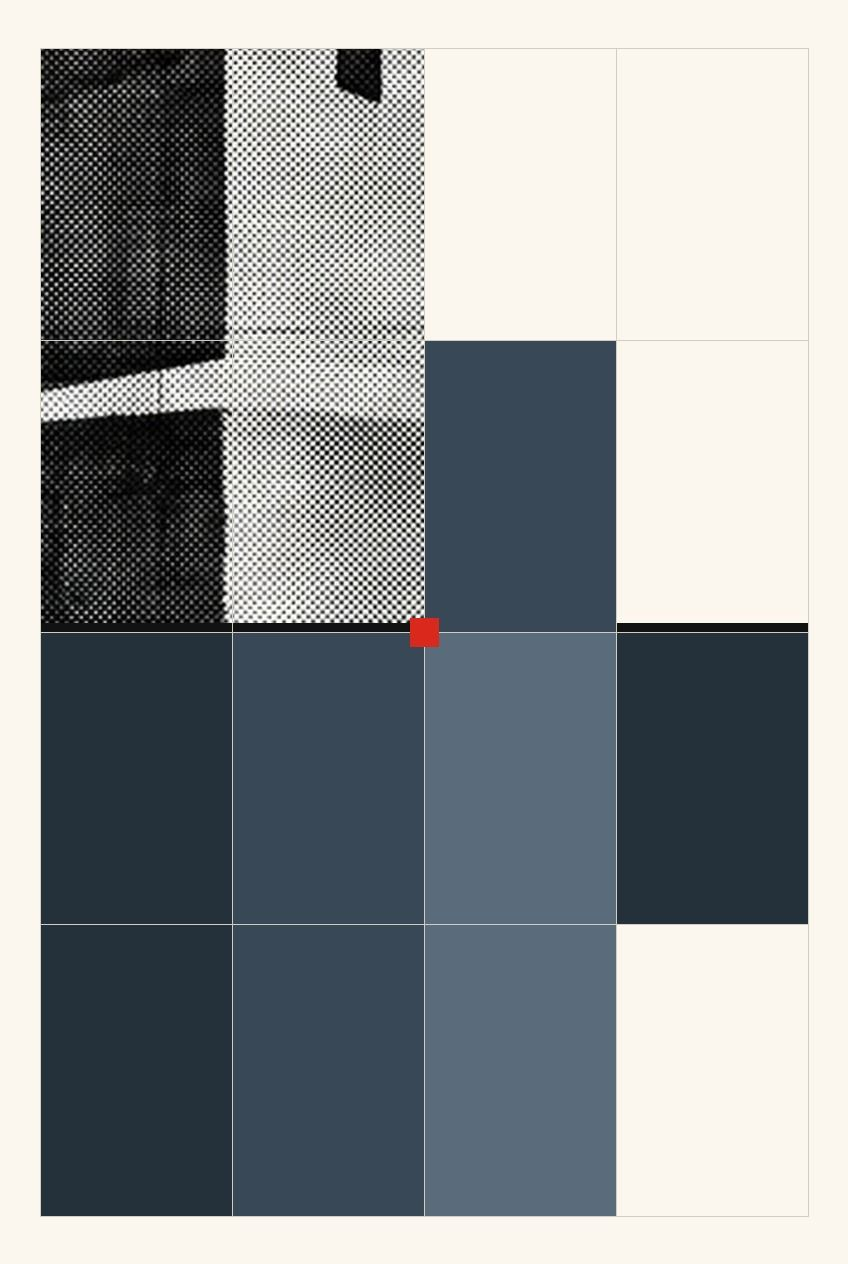
\includegraphics[width=\linewidth,height=0.92in,keepaspectratio]{plates/swiss/landmark-01.jpg}}%
    }{%
      \PackageError{pd-book-contents}{Missing chapter plate \pd@tocplatepath}%
        {Restore the chapter's edition-specific plate before building the Book.}%
    }%
  }}
% A fresh page for a part keeps its existing art and the first chapter together.
% The image is a visual locator for the same part plate encountered in the body.
\renewcommand*\l@part[2]{%
  \ifnum\pd@tocpart=0
    \par\addvspace{24pt}%
  \else
    \ifnum\pd@tocpart>\pdpartcount
      \Needspace*{14\baselineskip}\addvspace{24pt}%
    \else\clearpage\fi
  \fi
  \advance\pd@tocpart\@ne
  \pd@tocafterparttrue
  \ifnum\pd@tocpart>\pdpartcount
    \def\pd@toccolor{hhink}%
    {\pdtextface\LARGE\bfseries #1\hfill #2\par}%
    \vspace{9pt}\noindent\rule{\linewidth}{0.7pt}\par\vspace{12pt}%
  \else
    \edef\pd@toccolor{\csname pd@tocpartcolor@\the\pd@tocpart\endcsname}%
    \noindent
    \begin{minipage}[t]{0.29\linewidth}\vspace{0pt}%
      \expandafter\pd@tocplate\expandafter{\csname pd@tocpartart@\the\pd@tocpart\endcsname}%
    \end{minipage}\hfill
    \begin{minipage}[t]{0.66\linewidth}\vspace{0pt}\pdtextface\raggedright
      {\Large\bfseries\color{\pd@toccolor}#1\par}%
      \vspace{7pt}%
      {\small\csname pd@tocpartblurb@\the\pd@tocpart\endcsname\par}%
      \vspace{7pt}{\small Part opens on page #2\par}%
    \end{minipage}\par
    \vspace{13pt}\noindent{\color{\pd@toccolor}\rule{\linewidth}{1.1pt}}\par\vspace{10pt}%
  \fi\nobreak}
\newcommand*\l@chapter[2]{%
  \ifnum\pd@tocpart=0
    \Needspace*{15\baselineskip}\addvspace{22pt}%
    \noindent\begin{minipage}[t]{0.23\linewidth}\vspace{0pt}%
      \expandafter\pd@tocchapterplate\expandafter{\csname pd@tocchapterart@0\endcsname}%
    \end{minipage}\hfill
    \begin{minipage}[t]{0.72\linewidth}\vspace{0pt}%
    \begingroup
      \pdtextface\large\bfseries\color{\pd@toccolor}%
      \parindent\z@\rightskip 2.5em\parfillskip -2.5em
      \let\numberline\pd@tocchapternumber
      #1\nobreak\hfill\makebox[2.5em][r]{#2}\par
    \endgroup\nobreak
    \vspace{5pt}%
    {\rmfamily\small\raggedright
      \csname pd@tocchapterclaim@0\endcsname\par
      \edef\pd@tocnotename{pd@tocchapternote@0}%
      \expandafter\ifx\csname\pd@tocnotename\endcsname\@empty\else
        \vspace{3pt}{\itshape\csname\pd@tocnotename\endcsname\par}%
      \fi}%
    \end{minipage}\par\nobreak\vspace{10pt}%
  \else
    \ifpd@tocafterpart\pd@tocafterpartfalse\else
      \Needspace*{15\baselineskip}\addvspace{22pt}%
    \fi
    \advance\pd@tocchapter\@ne
    \noindent\begin{minipage}[t]{0.23\linewidth}\vspace{0pt}%
      \ifcsname pd@tocchapterart@\the\pd@tocchapter\endcsname
        \expandafter\pd@tocchapterplate\expandafter{\csname pd@tocchapterart@\the\pd@tocchapter\endcsname}%
      \fi
    \end{minipage}\hfill
    \begin{minipage}[t]{0.72\linewidth}\vspace{0pt}%
    \begingroup
      \pdtextface\large\bfseries\color{\pd@toccolor}%
      \parindent\z@\rightskip 2.5em\parfillskip -2.5em
      \let\numberline\pd@tocchapternumber
      #1\nobreak\hfill\makebox[2.5em][r]{#2}\par
    \endgroup\nobreak
    \vspace{5pt}%
    {\rmfamily\small\raggedright
      \ifcsname pd@tocchapterclaim@\the\pd@tocchapter\endcsname
        \csname pd@tocchapterclaim@\the\pd@tocchapter\endcsname\par
      \fi
      \edef\pd@tocnotename{pd@tocchapternote@\the\pd@tocchapter}%
      \ifcsname\pd@tocnotename\endcsname
        \expandafter\ifx\csname\pd@tocnotename\endcsname\@empty\else
          \vspace{3pt}{\itshape\csname\pd@tocnotename\endcsname\par}%
        \fi
      \fi}%
    \end{minipage}\par\nobreak\vspace{10pt}%
  \fi}
\newcommand{\pd@tocchapternumber}[1]{#1\enspace}
% A quiet number gutter and one aligned page column. Subsections indent only
% their numbers; long titles keep a generous measure and wrap as hanging text.
\renewcommand*\l@section[2]{%
  \addvspace{5pt}\begingroup\pdtextface\normalsize\bfseries
    \@dottedtocline{1}{0pt}{3.8em}{#1}{#2}%
  \endgroup\nobreak}
\renewcommand*\l@subsection[2]{%
  \begingroup\pdtextface\small
    \@dottedtocline{2}{1.2em}{4.4em}{#1}{#2}%
  \endgroup}
\renewcommand*\l@subsubsection[2]{%
  \begingroup\color{hhgray}\pdcaptionface\footnotesize
    \@dottedtocline{3}{2.4em}{5em}{#1}{#2}%
  \endgroup}
\fancypagestyle{pdcontentsopening}{%
  \fancyhf{}%
  \fancyfoot[LE,RO]{\rmfamily\small\thepage}%
  \renewcommand{\headrulewidth}{0pt}%
}
\newcommand{\pdtableofcontents}{%
  \clearpage
  \newgeometry{inner=0.8in,outer=0.2in,top=0.85in,bottom=0.95in}%
  \begingroup
    \rmfamily\normalsize\color{hhink}%
    \parindent\z@\parskip\z@
    % Frontmatter roman folios need more room than the class's 1.55em gutter.
    \renewcommand\@pnumwidth{2.8em}\renewcommand\@tocrmarg{3.8em}%
    \setlength{\headwidth}{\textwidth}%
    \fancyhf{}\fancyhead[LE,RO]{\rmfamily\small Contents}%
    \fancyfoot[LE,RO]{\rmfamily\small\thepage}%
    \hypersetup{linkcolor=hhink}%
    \pd@tocpart=0 \pd@tocchapter=0 \pd@tocafterpartfalse
    \thispagestyle{pdcontentsopening}%
    \phantomsection\label{book:contents}%
    \pdfbookmark[0]{Contents}{book.contents}%
    {\pddisplayface\Huge\bfseries Contents\par}%
    \vspace{10pt}\noindent\rule{\linewidth}{1.1pt}\par\vspace{14pt}%
    {\pdtextface\large The complete argument: the foundations of Chapter~0, then \pdchaptercount{} chapters.\par}%
    \vspace{6pt}%
    \begin{minipage}{0.84\linewidth}\rmfamily\normalsize\raggedright
      Every chapter, section and subsection is listed here, followed by
      solutions, the result atlas, reference material and image credits.
      Titles and page numbers lead directly to their place in the book.
    \end{minipage}\par\vspace{20pt}%
    \@starttoc{toc}%
    \clearpage
  \endgroup
  \restoregeometry
}
\makeatother

% Hyperlink and cross-reference discipline (must stay last).
% Shared hyperlink and cross-reference discipline for the Book and its chapters.
% Load this LAST in every preamble: cleveref must follow hyperref and amsthm.
% hyperref itself is loaded earlier with [backref=page] (a load-time option).
% Twin copy under book/figures/ (byte-identical; checked by
% scripts/generate-mega-whitepaper.test.mjs).
%
% What a reader gets: live links on chapter titles, section numbers, theorems,
% figures, tables, equations, page numbers, and citations; PDF bookmarks three
% levels deep; and, at the end of every bibliography entry, the pages that cite it.
% Links are quiet: a warm dark ink one step lighter than body text, so the
% four part hues keep their meaning and an inline chapter title never competes
% with the part it sits in. Chrome pages (the front-matter map, part openers)
% recolor their own links locally.
\hypersetup{
  colorlinks=true,
  linkcolor=pdinkmuted,
  citecolor=pdinkmuted,
  urlcolor=pdinkmuted,
  filecolor=pdinkmuted,
  anchorcolor=pdink,
  bookmarksnumbered=true,
  bookmarksdepth=3,
  bookmarksopen=true,
  bookmarksopenlevel=1,
  breaklinks=true,
  linktoc=all,
  pdfauthor={Erich Owens},
  pdftitle={\pdchaptertitle},
  pdfsubject={\pdeditiontitle: \pdeditionsubtitle},
}

% Title-based chapter references. \pdchaplink{prefix}{text} is a live link to
% the chapter inside the Book (the Book's preamble defines it before loading this
% file); in a standalone chapter it is plain text. Prose uses \pdchapref, which
% sets the title in italics; the locator map uses \pdchaplink directly.
\providecommand{\pdchaplink}[2]{#2}
\DeclareRobustCommand{\pdchapref}[2]{\pdchaplink{#1}{\emph{#2}}}

% \ifpdbook -- true in the assembled Book, false otherwise.
%
% WHY THIS EXISTED. A drawing that two chapters both \input prints twice in the
% Book, under two figure numbers. The fix is for the chapter that develops the
% idea to keep the figure and the other to point at it -- but the standalone
% edition of a chapter had nowhere to point, and rewriting the prose outright
% removed five figures from harbor-economy-whitepaper.pdf and left it telling a
% conference reader that a ceremony is "drawn in The Federated Harbor", a
% document that reader did not have.
%
% WHERE IT STANDS NOW. The per-chapter PDFs are retired: the Book is the one
% document, so \ifpdbook is true in every build that renders, and the \else
% branches are source with no output. They are still here, and still read by
% check_duplicate_figures.py (which must not count an \else \input as a Book
% input) -- but nothing prints them, and nothing new should be put in one.
% Whether to delete them is an open question; see the retirement PR.
%
% The divergence was per-build. A CONDITIONAL and not a two-argument macro:
% the generator inlines each \input, so a figure branch is a whole table or
% tikzpicture, and as a macro argument that is scanned as one token list --
% which is how \pdinbook produced "runaway argument" on the first attempt.
% \ifpdbook skips the untaken branch at the TeX level instead.
%
% Declared unconditionally and defaulting FALSE, which is the standalone
% answer. The Book's preamble sets \pdbooktrue immediately after loading
% this file. A guard here would have to mention \ifpdbook or \newif inside a
% branch TeX may skip, and a conditional token in skipped text is counted as
% a nested \if -- which is how two attempts at a guard both produced
% "Incomplete \ifdefined". Ordering is cheaper than cleverness.
\newif\ifpdbook

% cleveref: "Theorem 3.1", "Figure 2.4", "Section 1.3", capitalised, never
% abbreviated, with the whole phrase clickable. Names are declared explicitly
% because the theorem environments are created before this file is loaded.
\usepackage[nameinlink,capitalise,noabbrev]{cleveref}
\crefname{pdchapter}{Chapter}{Chapters}
\crefname{part}{Part}{Parts}
\crefname{appendix}{Appendix}{Appendices}
\crefname{definition}{Definition}{Definitions}
\crefname{theorem}{Theorem}{Theorems}
\crefname{lemma}{Lemma}{Lemmas}
\crefname{proposition}{Proposition}{Propositions}
\crefname{corollary}{Corollary}{Corollaries}
\crefname{conjecture}{Conjecture}{Conjectures}
\crefname{property}{Property}{Properties}
\crefname{protocol}{Protocol}{Protocols}
\crefname{lsprotocol}{Protocol}{Protocols}
\crefname{stpprotocol}{Protocol}{Protocols}
\crefname{heprotocol}{Protocol}{Protocols}
\crefname{remark}{Remark}{Remarks}
\crefname{lstlisting}{Listing}{Listings}
\crefname{exercise}{Exercise}{Exercises}
\crefname{solution}{Solution}{Solutions}
\Crefname{pdchapter}{Chapter}{Chapters}
\Crefname{lstlisting}{Listing}{Listings}
\Crefname{exercise}{Exercise}{Exercises}
\Crefname{solution}{Solution}{Solutions}

% Back-references: "^ Cited on pages 12, 40, and 87." after every bibliography
% entry, each page number a live link back to the page that cited the work.
% Distinct pages only (#3/#4).
%
% The page numbers used to be wrapped in \color{hhgray} along with the words,
% which painted over the link colour hyperref had just given them: the links
% were there -- 29 annotations on a typical bibliography page -- and looked
% exactly like the grey prose around them, so nobody knew they could click.
% Restoring the quiet link colour would not have fixed it either; pdinkmuted
% against hhgray is 1.53:1, which is no signal at footnote size.
%
% So the numbers take pdcobalt (7.55:1 on the cream, and a hue a reader cannot
% mistake for grey), and the line opens with the return arrow this book already
% uses to send a solution back to its exercise. This is a deliberate exception
% to the quiet-link discipline above, and the reason is that back-matter
% navigation is the one place where the link IS the content: in prose the
% surrounding sentence tells you a phrase is a destination, and in a
% bibliography nothing does.
\renewcommand*{\backref}[1]{}
\renewcommand*{\backrefalt}[4]{%
  \ifcase #3\relax
  \or {\footnotesize{\color{hhgray}$\uparrow$~Cited on page}~{\hypersetup{linkcolor=pdcobalt}#4}{\color{hhgray}.}}%
  \else {\footnotesize{\color{hhgray}$\uparrow$~Cited on pages}~{\hypersetup{linkcolor=pdcobalt}#4}{\color{hhgray}.}}%
  \fi}
\renewcommand*{\backrefsep}{, }
\renewcommand*{\backreftwosep}{ and }
\renewcommand*{\backreflastsep}{, and }

% \ifpdbook is declared (false) in pd-hyperlinks; the Book turns it on here,
% AFTER the load, so nothing has to guard the \newif. It selects the Book
% branch wherever a chapter and its standalone paper must diverge -- a
% figure the Book prints once and cross-references, which the paper carries
% its own copy of.
\pdbooktrue

% ---------------------------------------------------------------------------
% Captioned exhibits must fit the text column: the outside margin is reserved
% for their captions. Record true ink width and warn on overflow; the matching
% PDF audit rejects it. Never hide an oversized figure by shrinking its type
% or moving its caption below it. The legacy spill/scale path below applies
% only to non-floating inline artwork and remains separately reviewable.
% ---------------------------------------------------------------------------
\usepackage{changepage}
\strictpagecheck
\newlength{\pdfullwidth}\setlength{\pdfullwidth}{\dimexpr\textwidth+\marginparsep+\marginparwidth\relax}
\makeatletter
% pgf hands every finished picture (tikzpicture, pgfplots axis, inline \tikz)
% to \pgfsys@typesetpicturebox with its width known; the hook decides where it
% goes. Nested pictures pass through untouched (their box is narrower than the
% line they sit in).
\newsavebox{\pd@picbox}
\let\pd@typesetpicturebox\pgfsys@typesetpicturebox
\def\pgfsys@typesetpicturebox#1{%
  \sbox{\pd@picbox}{\pd@typesetpicturebox#1}%
  % Figure-band recording for \pd@placemargin's centering (pd-pedagogy.tex):
  % from THIS box's own \ht/\dp, not from \pagetotal at \end{figure}. The
  % latter was tried first and does not work -- for an [H] float the
  % package defers inserting the box into the main vertical list past
  % \end{figure} itself, so \pagetotal read there (even settled) still
  % under-reads by the whole figure and \pd@figbot came out equal to
  % \pd@figtop on every figure measured. \pagetotal HERE, mid-paragraph
  % while pgf is still handing us the finished picture box, is the page
  % height immediately above where this box is about to be placed, and the
  % box's own \ht+\dp is its true rendered height regardless of how (or
  % whether) it gets rescaled below -- both read before any resizing, which
  % is fine: \pd@placemargin only wants the figure's vertical band, and
  % \resizebox below does not change a box's VERTICAL position, only its
  % size, and \centering does not move a box vertically at all.
  \ifpdmargincolumn
    \xdef\pd@figpage{\number\value{page}}%
    \global\pd@figtop=\pagetotal
    \global\pd@figbot=\dimexpr\pagetotal+\ht\pd@picbox+\dp\pd@picbox\relax
  \fi
  % the box has no width of its own yet; pgf sets it from the bounding box
  \@tempdima=\dimexpr\pgf@picmaxx-\pgf@picminx\relax
  \ifpd@captionfloat
    \ifdim\@tempdima>\pd@exhibitinkwidth
      \global\pd@exhibitinkwidth=\@tempdima\fi
  \fi
  \ifdim\@tempdima>\dimexpr\linewidth+1pt\relax
    \ifpd@captionfloat
      % The outer margin belongs to the caption. Preserve the bad geometry
      % for the audit; never conceal it by shrinking type or dropping captions.
      \PackageWarning{pd-book}{PD-EXHIBIT-WIDE: \@captype\space
        \@nameuse{the\@captype}; width=\the\@tempdima; limit=\the\linewidth}%
      \makebox[\linewidth][c]{\usebox{\pd@picbox}}%
    \else
    \ifdim\linewidth<\dimexpr\textwidth-1pt\relax
      \ifpdmarginevidence
        \PackageError{pd-book}{Margin evidence exceeds its native width}%
          {Redraw to marginparwidth; shrinking labels is not permitted.}%
        \usebox{\pd@picbox}%
      \else
      % inside a minipage, a margin note or a table cell: fit the box we are in
      \PackageWarning{pd-book}{picture \the\wd\pd@picbox\space wide scaled to a \the\linewidth\space box}%
      \resizebox{\linewidth}{!}{\usebox{\pd@picbox}}%
      \fi
    \else
      \ifdim\wd\pd@picbox>\pdfullwidth
        \PackageWarning{pd-book}{picture \the\wd\pd@picbox\space wide scaled to the full width}%
        \sbox{\pd@picbox}{\resizebox{\pdfullwidth}{!}{\usebox{\pd@picbox}}}%
      \else
        \PackageInfo{pd-book}{picture \the\wd\pd@picbox\space wide set full width}%
      \fi
      % Strict page checking records the box's shipped page in the aux file,
      % so a floated picture uses its physical leaf rather than the page TeX
      % happened to be composing when the hook fired. Odd rectos spill right;
      % even versos spill left. The text measure never shrinks to make room.
      \checkoddpage
      \ifoddpage
        \makebox[\textwidth][l]{\usebox{\pd@picbox}}%
      \else
        \makebox[\textwidth][r]{\usebox{\pd@picbox}}%
      \fi
    \fi
    \fi
  \else
    \usebox{\pd@picbox}%
  \fi}
\NewDocumentCommand\pdpagecentered{O{\pdfullwidth} m}{%
  \par\noindent\checkoddpage
  \makebox[\textwidth][c]{%
    \ifoddpage\hspace*{0.45in}\else\hspace*{-0.45in}\fi
    \makebox[#1][c]{#2}%
  }\par
}
\NewDocumentCommand\pdpagecaption{O{} m O{}}{%
  \par\vspace{6pt}%
  \begingroup
  \let\pd@captiontype\relax
  \pd@routecaptionfalse
  \noindent\checkoddpage
  \makebox[\textwidth][c]{%
    \ifoddpage\hspace*{0.45in}\else\hspace*{-0.45in}\fi
    \begin{minipage}{\dimexpr\pdfullwidth-0.2in\relax}%
      \if\relax\detokenize{#1}\relax\caption{#2}\else\caption[#1]{#2}\fi
      \if\relax\detokenize{#3}\relax\else\label{#3}\fi
    \end{minipage}%
  }%
  \endgroup
  \par
}
% Captioned exhibits use the same owner inventory and outside-margin route.
% A caller cannot opt out by calling a historical wide-caption helper.
\NewDocumentCommand\pdwidecaption{O{} m O{}}{%
  \if\relax\detokenize{#1}\relax\caption{#2}\else\caption[#1]{#2}\fi
  \if\relax\detokenize{#3}\relax\else\label{#3}\fi
}
\makeatother

% Book-owned openings and handoffs. The chapter sources remain independently
% buildable; these rails exist only in the Book. They are keyed by chapter
% prefix (see book/textbook.json), never by position, so reordering the
% book moves a chapter's rails with it. The handoff text, however, is written
% for the order the book is in: it names the chapter that comes next.
%
% An opening rail sits at the top of a chapter's first body page. Its heading
% is the chapter's question (from textbook.json, the same line the opener page
% set large); its body is the lede: the scene, in two or three sentences,
% before the chapter's own first section begins.

\newcommand{\pdbookrail}[2]{%
  \par\addvspace{12pt}%
  % A short opening/handoff is one paragraph, not a page-turn destination
  % for its last two lines. Keep the accent and its complete prose together.
  \noindent\begin{minipage}{\linewidth}
  % Keep question and handoff prose free of stretched interword spacing.
  \raggedright
  \noindent{\color{\pdcurrentchaptercolor}\rule{2.5em}{1.5pt}}\par
  \vspace{0.12cm}%
  \noindent{\small\scshape\bfseries\color{hhink}#1}\enspace
  {\small #2}\par
  \end{minipage}\par\addvspace{12pt}%
}

% ---- Part I: The Machine -------------------------------------------------

\newcommand{\pdchapteropeningswk}{%
  \pdbookrail{\pdchapterquestion}{%
    Alice's workers have two repairs based on revision~7. The first question is
    whether the second may still write after the first commits. This chapter
    locates the admission boundary, traces a stale request and a crash, and
    distinguishes a recorded conflict from a prevented effect.}%
}

\newcommand{\pdchapterhandoffswk}{%
  \pdbookrail{What \pdchapref{anchor}{The Anchor Protocol} receives}{%
    The repair now has a work-unit record, version checks and a stated recovery
    contract. These mechanisms distinguish a current proposal from a stale one;
    they do not determine who owns the repository. Next Bob must grant Alice
    precisely the authority needed for the job, including what her workers may
    inherit.}%
}

\newcommand{\pdchapteropeninganchor}{%
  \pdbookrail{\pdchapterquestion}{%
    Bob permits a checkout repair, not an unrelated migration or deployment.
    Alice delegates part of that work to Heron. This chapter follows the grant
    through signing, narrowing, presentation and revocation. The receiver must
    verify both the credential and its authority over the requested resource.}%
}

\newcommand{\pdchapterhandoffanchor}{%
  \pdbookrail{What \pdchapref{sealed}{The Sealed Harbor} receives}{%
    A verified grant can identify the permitted resource and action. It does
    not answer every disclosure question. Suppose diagnosis needs Derek's
    private checkout records and Erin's private model: neither owner has given
    Bob or Alice unrestricted access. The next chapter specifies how an answer
    may leave while their inputs remain subject to separate release policies.}%
}

\newcommand{\pdchapteropeningsealed}{%
  \pdbookrail{\pdchapterquestion}{%
    Derek supplies confidential records; Erin supplies the diagnostic model.
    They want a useful checkout diagnosis without releasing either input to
    the other party. We first write down the contract both owners sign and trace the permitted
    output, then state the channel, host and verifier assumptions needed to
    justify the confidentiality claims.}%
}

\newcommand{\pdchapterhandoffsealed}{%
  \pdbookrail{What \pdchapref{ls}{The Legible Swarm} receives}{%
    Alice may receive a permitted diagnosis without seeing the private evidence
    behind it. Other evidence is visible but too voluminous to read in full.
    These are different limits. The next chapter asks which observations a
    supervisor needs to distinguish a real repair from a deleted test or an
    overbroad patch, and how a summary should direct that inspection.}%
}

% ---- Part II: The Operator -----------------------------------------------

\newcommand{\pdchapteropeningls}{%
  \pdbookrail{\pdchapterquestion}{%
    Drake deletes the failing test. Wren fixes the defect but includes an
    unrelated migration. Heron contributes an acceptable repair. All three can
    produce an encouraging status line. This chapter asks what Alice must
    inspect, which records a successor needs, and how those demands compete
    for limited attention. Each bound uses an explicit observation model.}%
}

\newcommand{\pdchapterhandoffls}{%
  \pdbookrail{What \pdchapref{stp}{From Spawn to Person} receives}{%
    The supervisor can now ask which artifact supports a claim and which
    uncertainty remains. Tomorrow, however, Heron's process may be gone.
    To attribute its contribution and recover what it still owes, the next
    chapter separates an execution instance from a persistent participant and
    the principal responsible for it.}%
}

% ---- Part III: The Person ------------------------------------------------

\newcommand{\pdchapteropeningstp}{%
  \pdbookrail{\pdchapterquestion}{%
    Heron's process exits before all of its work is settled. A replacement can
    load the patch, but a new process label does not say which obligations or
    sanctions remain. This chapter defines the continuity needed to connect
    those records, then tests what reputation can and cannot mean under reset,
    migration and changing execution models.}%
}

\newcommand{\pdchapterhandoffstp}{%
  \pdbookrail{What \pdchapref{he}{The Harbor Economy} receives}{%
    A persistent participant links the repair to a responsible principal and
    retained outcomes. It does not make the work valuable or the reports true.
    The next chapter gives Bob and Alice an explicit purchase contract, with
    separate payment, collateral, evidence and settlement rules.}%
}

% ---- Part IV: The Market -------------------------------------------------

\newcommand{\pdchapteropeninghe}{%
  \pdbookrail{\pdchapterquestion}{%
    Bob buys the repair from Alice, who may also lease a runtime and use a
    metered skill. A labor price alone does not determine what each party
    receives after success, partial delivery or failure. This chapter follows
    those amounts through a worked ledger before generalizing the allocation,
    verification and incentive questions.}%
}

\newcommand{\pdchapterhandoffhe}{%
  \pdbookrail{What \pdchapref{bonded}{The Bonded Commons} receives}{%
    The contract names the parties, reserves and settlement rule. A disputed
    result still needs a procedure: who may submit evidence, who decides, and
    what remedy the decision authorizes. The next chapter keeps those questions
    separate from the immediate recovery of a worker that has gone silent.}%
}

\newcommand{\pdchapteropeningbonded}{%
  \pdbookrail{\pdchapterquestion}{%
    Heron's heartbeat stops while its contribution is being reviewed. Alice
    needs to recover the work; Bob may also contest whether the contract was
    satisfied. Silence alone decides neither question. This chapter develops
    recovery, adjudication and settlement as distinct procedures, then checks
    their stated accounting and incentive conditions.}%
}

\newcommand{\pdchapterhandoffbonded}{%
  \pdbookrail{What \pdchapref{fh}{The Federated Harbor} receives}{%
    The local institution now has separate rules for admission, recovery,
    evidence, adjudication and settlement. The repair must next run on a
    staging host governed by another operator. The final chapter asks which
    records travel, which authority must be granted there, and which
    disagreements the available observations can expose.}%
}

\newcommand{\pdchapteropeningfh}{%
  \pdbookrail{\pdchapterquestion}{%
    A staging operator receives the repair's signed receipts. They can help
    establish what an identified sender reported; they do not grant access to
    the staging machine. This chapter follows local authorization across the
    boundary, then asks when communication paths can witness inconsistent
    reports and when they leave a fault unobservable.}%
}

\newcommand{\pdchapterhandofffh}{%
  \pdbookrail{The conclusion of the book}{%
    The checkout job has acquired a sequence of inspectable contracts: what
    may change, who may authorize it, what may be disclosed, what evidence a
    reader needs, what survives replacement, how money is conserved, and who
    decides a dispute. Each contract preserves its own assumptions. Together
    they provide questions and mechanisms for designing accountable work;
    the book does not establish that every proposed component has been
    deployed or that their composition removes every failure.}%
}

% References belong beside the discussion throughout the assembled Book.
% The registry remains build data; standalone chapter behavior is unchanged.
\providecommand{\pdEnableMarginCitations}{1}
\ifdefined\pdEnableMarginCitations
  % Book-only citations. Load AFTER pd-margin-layout, before document.
% Sources are set in the margin beside their first use, and listed once more,
% alphabetically, in the back matter (pdreferences, at the end of this file).
% Enabled by default in the assembled Book; standalone chapters are unchanged.
% Public references are unnumbered. Registry integers are accounting data,
% never superscript callouts or bold numerals in the reader's margin.
\makeatletter
\newif\ifpdbookinmargin
\newif\ifpdbookcitereplay
\newcommand{\pdbookmargincontext}[1]{\begingroup\pdbookinmargintrue #1\endgroup}
\NewCommandCopy\pdbookoriginalmarginregister\pdmarginregister
\RenewDocumentCommand\pdmarginregister{m +m}{%
  \pdbookoriginalmarginregister{#1}{\pdbookmargincontext{#2}}}
% Captions/portraits/exhibits are measured BEFORE they reach the allocator.
% Mark that earlier measurement too: a citation belongs to its owning box.
\let\pdbookoriginalstorecaption\pd@storecaption
\renewcommand{\pd@storecaption}[1]{%
  \pdbookmargincontext{\pdbookoriginalstorecaption{#1}}}
\let\pdbookoriginalmarginfigure\pdmarginfigure
\renewcommand{\pdmarginfigure}[2]{%
  \pdbookmargincontext{\pdbookoriginalmarginfigure{#1}{#2}}}
\NewCommandCopy\pdbookoriginalmarginexhibit\pdmarginexhibit
\RenewDocumentCommand\pdmarginexhibit{m m +m +m}{%
  \pdbookmargincontext{\pdbookoriginalmarginexhibit{#1}{#2}{#3}{#4}}}
% A contents/figure-list replay must not consume first use or emit a note.
\let\pdbookoriginalstarttoc\@starttoc
\renewcommand{\@starttoc}[1]{%
  \begingroup\pdbookcitereplaytrue\pdbookoriginalstarttoc{#1}\endgroup}
% tabularx evaluates its body several times while finding column widths.
% Its trial argument runs INSIDE the discarded trial box, so this flag is
% local to measurement and cannot consume first use or register ghost notes.
% https://github.com/latex3/latex2e/blob/develop/required/tools/tabularx.dtx
\let\pdbookoriginalTXtrial\TX@trial
\def\TX@trial#1{\pdbookoriginalTXtrial{\pdbookcitereplaytrue #1}}
\providecommand{\pdbookcitationrecord}[4]{}
\ExplSyntaxOn
\prop_new:N \g_pd_book_cite_number_prop
\prop_new:N \g_pd_book_cite_full_prop
\prop_new:N \g_pd_book_cite_short_prop
\prop_new:N \g_pd_book_cite_seen_prop
\prop_new:N \g_pd_book_cite_page_prop
\int_new:N \g_pd_book_cite_occurrence_int
\tl_new:N \l_pd_book_cite_page_tl
\clist_new:N \l_pd_book_cite_fresh_clist
\bool_new:N \l_pd_book_cite_first_bool
\cs_new_protected:Npn \pd_book_cite_require:n #1
  {\prop_if_in:NnF \g_pd_book_cite_number_prop {#1}
    {\PackageError{pd-book-citations}{Unregistered~source:~#1}
      {Register~the~source.~Never~silently~drop~a~citation.}}}
\NewDocumentCommand\pdbookreference{m m +m +m}
  {\prop_if_in:NnTF \g_pd_book_cite_number_prop {#1}
    {\PackageError{pd-book-citations}{Duplicate~source:~#1}
      {Use~one~canonical~entry~per~source.}}
    {\prop_gput:Nnn \g_pd_book_cite_number_prop {#1}{#2}
     \prop_gput:Nnn \g_pd_book_cite_full_prop {#1}{#3}
     \prop_gput:Nnn \g_pd_book_cite_short_prop {#1}{#4}}}
\cs_new_protected:Npn \pd_book_cite_entry:n #1
  {\pd_book_cite_require:n {#1}
   \par\noindent
   \prop_if_in:NnTF \g_pd_book_cite_seen_prop {#1}
    {\hyperlink{pdbook-source-#1}{\prop_item:Nn \g_pd_book_cite_short_prop {#1}}
     \iow_log:x {PD-BOOK-SOURCE:~key=#1,~form=repeat}}
    {\hypertarget{pdbook-source-#1}{}%
     \prop_item:Nn \g_pd_book_cite_full_prop {#1}
     \prop_gput:Nnn \g_pd_book_cite_seen_prop {#1}{1}
     \iow_log:x {PD-BOOK-SOURCE:~key=#1,~form=full}}}
\cs_new_protected:Npn \pd_book_cite_text:nn #1#2
  {\begingroup\mdseries\upshape
   \let\newblock\space
   \bool_set_true:N \l_pd_book_cite_first_bool
   \clist_map_inline:nn {#2}
     {\bool_if:NF \l_pd_book_cite_first_bool {\par\smallskip}
      \bool_set_false:N \l_pd_book_cite_first_bool
      \pd_book_cite_entry:n {##1}}
   \tl_if_blank:nF {#1}{\par\nobreak\emph{Cited:~#1.}}
   \par\endgroup}
\cs_new_protected:Npn \pd_book_cite_record:nnn #1#2#3
  {\int_gincr:N \g_pd_book_cite_occurrence_int
   \exp_args:Nx \zsavepos {pdc-\int_use:N\g_pd_book_cite_occurrence_int}
   \iow_log:x {PD-BOOK-CITE:~occurrence=\int_use:N\g_pd_book_cite_occurrence_int,
      ~keys=\tl_to_str:n{#2},~context=#3,~locator=\tl_to_str:n{#1}}
   \protected@write\@auxout{}
     {\string\pdbookcitationrecord{\int_use:N\g_pd_book_cite_occurrence_int}
       {#2}{#3}{\unexpanded{#1}}}}
% Repeated marks on the same physical page share one readable margin source.
% Use shipped positions from the prior pass, never the current page counter
% (which is wrong inside a paragraph or delayed float). Locators get their own
% note so consolidation cannot erase the specific passage being cited.
\cs_new_protected:Npn \pd_book_cite_note:nn #1#2
  {\tl_set:Nx \l_pd_book_cite_page_tl
    {\zref@extractdefault{pdc-\int_use:N\g_pd_book_cite_occurrence_int}{abspage}{0}}
   \clist_clear:N \l_pd_book_cite_fresh_clist
   \clist_map_inline:nn {#2}
    {\tl_set:Nx \l_tmpa_tl {\tl_use:N\l_pd_book_cite_page_tl / ##1}
     \bool_set_false:N \l_tmpa_bool
     \tl_if_eq:NnT \l_pd_book_cite_page_tl {0}{\bool_set_true:N\l_tmpa_bool}
     \tl_if_blank:nF {#1}{\bool_set_true:N\l_tmpa_bool}
     \prop_if_in:NVF \g_pd_book_cite_page_prop \l_tmpa_tl {\bool_set_true:N\l_tmpa_bool}
     \bool_if:NT \l_tmpa_bool
       {\clist_put_right:Nn \l_pd_book_cite_fresh_clist {##1}
        \prop_gput:NVn \g_pd_book_cite_page_prop \l_tmpa_tl {1}}}
   \clist_if_empty:NTF \l_pd_book_cite_fresh_clist
     {\pdmarginreserveslot
      \iow_log:x {PD-BOOK-CITE-SHARED:~occurrence=\int_use:N\g_pd_book_cite_occurrence_int}}
     {\exp_args:NnV \pd_book_cite_register:nn {#1}\l_pd_book_cite_fresh_clist}}
\cs_new_protected:Npn \pd_book_cite_register:nn #1#2
  {\pdmarginregister{citation}{\pd_book_cite_text:nn{#1}{#2}}
   \iow_log:x {PD-BOOK-CITE-BOX:~occurrence=\int_use:N\g_pd_book_cite_occurrence_int,
     ~id=\pdmarginlastid,~keys=\tl_to_str:n{#2}}}
\NewDocumentCommand\pdbookcite{O{} m}
  {\ifpdbookcitereplay
     \unskip
   \else
     \ifpdbookinmargin
       \pd_book_cite_record:nnn{#1}{#2}{embedded}%
       \par\smallskip\pd_book_cite_text:nn{#1}{#2}%
     \else
       % Existing sources use word~\cite{key}. Remove that obsolete gap so
       % punctuation does not acquire an extra space when the callout vanishes.
       \unskip
       \pd_book_cite_record:nnn{#1}{#2}{body}%
       \pd_book_cite_note:nn{#1}{#2}%
     \fi
   \fi}
\AtEndDocument{\iow_log:x {PD-BOOK-CITE-SUMMARY:~occurrences=
  \int_use:N\g_pd_book_cite_occurrence_int,~sources=
  \prop_count:N\g_pd_book_cite_seen_prop,~registered=
  \prop_count:N\g_pd_book_cite_number_prop}}
\ExplSyntaxOff
% An authored sidenote carries its own thought, not a displaced bibliography.
% Sources inside it are credited in the same measured box. No nested note,
% arbitrary public number or duplicate inline callout is created.
\RenewDocumentCommand\pdsourceaside{+m}{\pdmarginregister{aside}{#1}}
\AtBeginDocument{%
  \typeout{PD-BOOK-CITE-CAPACITY: \the\textheight}%
  \RenewDocumentCommand\pdcite{O{} m}{\pdbookcite[#1]{#2}}%
  \RenewDocumentCommand\cite{O{} m}{\pdbookcite[#1]{#2}}%
}
% The reference list in the back matter: every source once, by first author,
% unnumbered like the margin entries, each one complete as its chapter wrote
% it. scripts/generate-mega-whitepaper.mjs writes the entries.
\newenvironment{pdreferences}
  {\begingroup\small\raggedright\let\newblock\space
   \setlength{\parindent}{0pt}\setlength{\parskip}{2.5pt plus 1pt}%
   \emergencystretch=2em}
  {\par\endgroup}
\newcommand{\pdreferenceentry}[1]{\par\hangindent=1.4em\hangafter=1\relax #1\par}
\makeatother

  \pdgeneratedinput{../.cache/whitepaper-build/coordination-papers-mega-volume/mega-volume-margin-references.tex}{margin references}
\fi
\hypersetup{
  pdftitle={\pdeditiontitle: \pdeditionsubtitle},
  pdfauthor={Erich Owens},
  pdfsubject={Eight chapters, in dependency order, on accountable autonomous work},
  pdfkeywords={supervisory control, multi-agent systems, capability security, coordination, accountability, federation}
}

\begin{document}
\hypersetup{pageanchor=false}
% The cover, imprint, frontispiece and epigraphs are physical pages i--iv, so
% their PDF page labels must be roman too; arabic labels 1--4 would collide
% with Chapter 0's folios.
\renewcommand{\thepage}{\roman{page}}
\begin{titlepage}
\pagecolor{hhpaper}\color{hhink}
\ifpdswiss
  % Swiss cover A (SWISS-BRIEF, C): the arcs block on the lower 56 per cent,
  % three type sizes on one left datum at 14 mm, the imprint in the foot.
  \pdswisscoverart
  \begin{tikzpicture}[remember picture,overlay,shift={(current page.north west)},x=1mm,y=-1mm]
    % The type block ends at about 28% of the 254mm page, which is the number
    % the cover plate's reserved band has to clear: see
    % scripts/whitepaper-plates/check_cover_title_band.py, which measures the
    % plate and fails the build rather than leaving it to the eye. Round 4a's
    % cover looked clean in a contact sheet, started its photograph 2% down,
    % and printed the subtitle over a container port.
    % All three lines live in the plate's reserved band, top-left, and the
    % image has the rest of the sheet. The imprint used to sit at the foot,
    % which put 9pt type over a halftone photograph that is 37% lighter than
    % luminance 140 -- neither black nor reversed white reads on that.
    \node[anchor=north west,inner sep=0pt,text width=145mm,align=left] at (14,14) {%
      {\pdcovergrotesk\fontsize{28}{33}\selectfont\bfseries\color{hhink}\spaceskip=0pt\xspaceskip=0pt%
       Governing AI Agents:\\[1.5mm]%
       The Harbor, the Person,\\and the Economy\par}%
      \vspace{5mm}%
      {\pdcovergrotesk\fontsize{11}{14}\selectfont\color{hhink}\spaceskip=0pt\xspaceskip=0pt%
       \pdeditionsubtitle\par}%
      \vspace{4mm}%
      {\pdcovergrotesk\fontsize{8.5}{11}\selectfont\color{hhgray}\spaceskip=0pt\xspaceskip=0pt%
       Erich Owens\quad\textperiodcentered\quad Curiositech\quad\textperiodcentered\quad Textbook Edition\par}%
    };
  \end{tikzpicture}
\else\ifpdtechnical
  % Technical cover: the engraving in the lower two thirds of the sheet, the
  % type in the paper above it, the sheet's frame and title block over all.
  \pdtechsheetplain{\pdeditiontitle}{Cover}%
  \begin{tikzpicture}[remember picture,overlay,shift={(current page.south west)},x=1in,y=1in]
    \IfFileExists{plates/technical/cover.jpg}{%
      \node[anchor=south,inner sep=0pt] at (3.5,1.55) {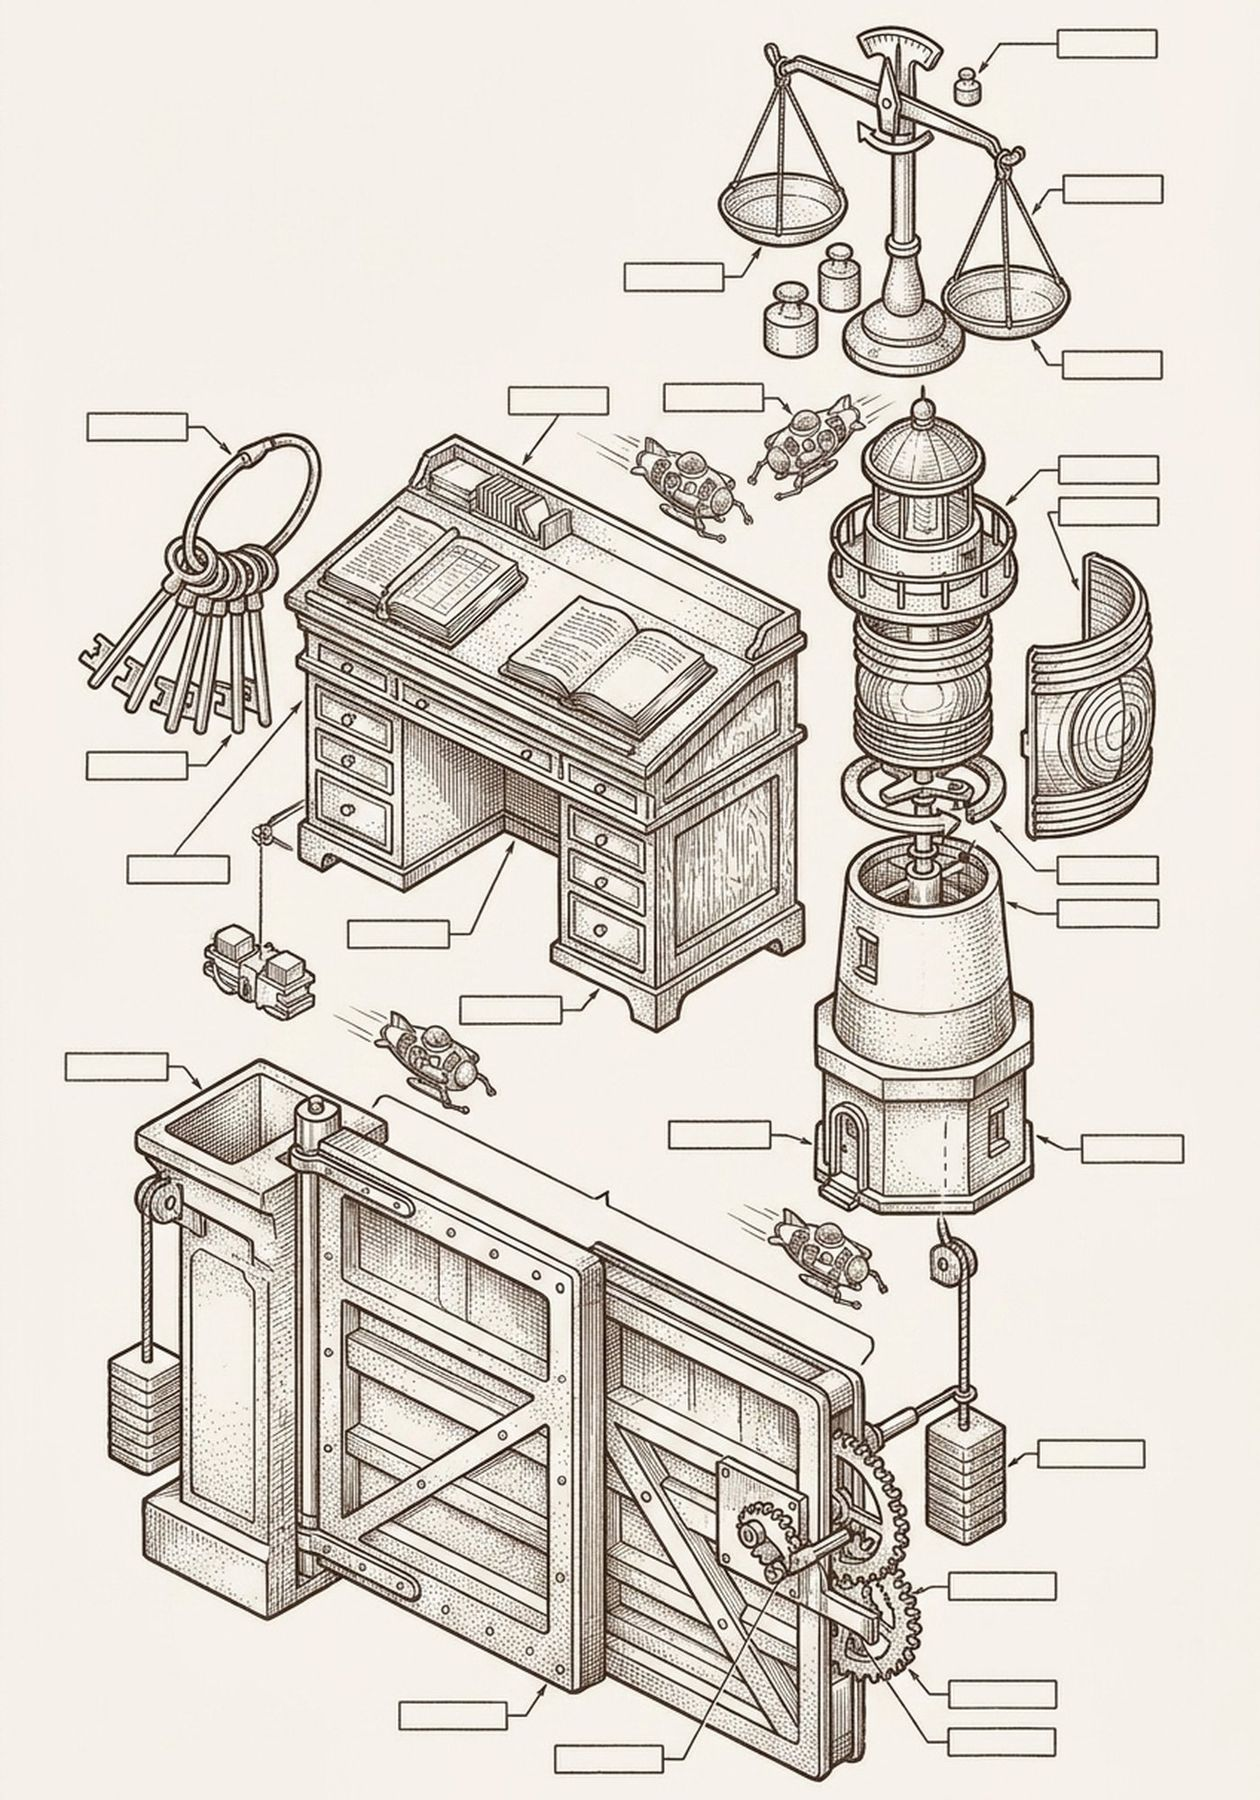
\includegraphics[height=4.55in]{plates/technical/cover.jpg}};}{}
    \node[anchor=north west,inner sep=0pt,text width=5.2in,align=left,font=\pdgrotesk\fontsize{24}{28}\selectfont,text=hhink] at (0.9,9.15) {\pdeditiontitle};
    \node[anchor=north west,inner sep=0pt,text width=5.2in,align=left,font=\pdgrotesk\fontsize{11}{14}\selectfont,text=hhink] at (0.9,7.8) {\pdeditionsubtitle};
    \node[anchor=north west,inner sep=0pt,font=\pdgrotesk\fontsize{9}{11}\selectfont,text=hhink] at (0.9,7.35) {Erich Owens\quad\textperiodcentered\quad Curiositech\quad\textperiodcentered\quad Textbook Edition};
  \end{tikzpicture}
\else
% Cover: the wash plate bleeds over the whole page; the type stays minimal and set in Times.
\IfFileExists{plates/jacket.jpg}{%
  \AddToShipoutPictureBG*{\AtPageLowerLeft{
\includegraphics[width=\paperwidth,height=\paperheight]{plates/jacket.jpg}}}}{}%
\vspace*{1.2cm}
\noindent\begin{minipage}{0.88\textwidth}
{\pdpartface\fontsize{30}{36}\selectfont\raggedright Governing AI Agents:\\[2mm] The Harbor, the Person,\\ and the Economy\par}
\vspace{0.6cm}
\noindent{\color{pdcobalt}\rule{0.24\textwidth}{1pt}}\par
\vspace{0.45cm}
{\pdpartface\itshape\fontsize{14.5}{19}\selectfont \pdeditionsubtitle\par}
\end{minipage}
\vfill
\noindent{\pdpartface\scshape\small Erich Owens\par\vspace{3pt}Curiositech\ \textperiodcentered\ Textbook Edition\par}
\vspace*{0.4cm}
\fi\fi
\end{titlepage}
% Imprint page: the claim, the ordering rule, and the publication data that the cover no longer carries.
\clearpage\thispagestyle{empty}\pagecolor{hhpaper}\color{hhink}
\vspace*{\fill}
\noindent\pdweightrule{0}{\textwidth}{2.6pt}\par
\vspace{0.6cm}
\noindent\begin{minipage}{0.96\textwidth}\small
{\large\bfseries\pdeditiontitle}\par\vspace{3pt}
{\color{hhgray}\pdeditionsubtitle}\par\vspace{10pt}
{\bfseries\pdeditionclaim}\par\vspace{6pt}
{\color{hhgray}This book follows that claim from one machine run by one human to work shared
across several owners, economic interests, and mutually distrustful systems. Its \pdchaptercountword{}
chapters are ordered by dependency: each chapter that proves a property comes after
the chapter that relies on it.}\par\vspace{12pt}
Erich Owens \textperiodcentered\ Curiositech LLC \textperiodcentered\ \texttt{engineering@portdaddy.dev}\par
Curiositech \textperiodcentered\ Version \pdeditionversion\ \textperiodcentered\ \pdeditiondate\ \textperiodcentered\ \url{https://portdaddy.dev/whitepaper}\par
\end{minipage}
\vspace*{1.0cm}
\clearpage
% Frontispiece: the plate faces the title matter, in the edition's own register.
%
% It used to be one maritime etching printed in all three editions and wrapped
% in \IfFileExists, which is two defects in four lines. The etching's vellum and
% cross-hatching in front of the Swiss edition's flat colour blocks announced
% that the character stops at the cover; and a missing plate printed NOTHING, so
% the book would have shipped without a frontispiece and told nobody -- the
% silent fallback the plate rule exists to forbid (see the \PackageError in
% coordination-papers-mega-volume-swiss-plates.tex, which this now matches).
\newcommand{\pdfrontispiece}[1]{%
  \IfFileExists{#1}{%
    \thispagestyle{empty}\pagecolor{hhpaper}\color{hhink}%
    \vspace*{\fill}
    \begin{center}\includegraphics[height=0.92\textheight,width=\textwidth,keepaspectratio]{#1}\end{center}
    \vspace*{\fill}
    \clearpage}{%
    \PackageError{coordination-papers-mega-volume}{Missing plate render #1}%
      {Generate this edition's frontispiece and place it at #1 before building.}}}
\ifpdswiss
  \pdfrontispiece{plates/swiss/frontispiece.jpg}
\else\ifpdtechnical
  \pdfrontispiece{plates/technical/frontispiece.jpg}
\else
  \pdfrontispiece{plates/frontispiece.jpg}
\fi\fi
\nopagecolor\color{hhink}

% Epigraphs leaf: Hobbes and von Neumann (verso, physical page iv)
\clearpage\thispagestyle{empty}\pagecolor{hhpaper}\color{hhink}
\vspace*{\fill}
\noindent\begin{minipage}{0.95\textwidth}\normalsize\itshape
``Nature (the art whereby God hath made and governes the world) is by the art of man, as in many other things, so in this also imitated, that it can make an Artificial Animal... For by art is created that great \textsc{Leviathan} called a \textsc{Common-Wealth}, or \textsc{State} (in latine \textsc{Civitas}) which is but an Artificiall Man; though of greater stature and strength than the Naturall, for whose protection and defence it was intended.''
\par\vspace{7pt}
\raggedleft\upshape\small--- \textbf{Thomas Hobbes}, \emph{Leviathan} (1651), Introduction
\end{minipage}

\vspace{1.1cm}

\noindent\begin{minipage}{0.95\textwidth}\normalsize\itshape
``Error is viewed, therefore, not as an extraneous and misdirected or misdirecting accident, but as an essential part of the process under consideration---its importance in the synthesis of automata being fully comparable to that of the factor which is normally considered, the intended and correct logical structure.''
\par\vspace{7pt}
\raggedleft\upshape\small--- \textbf{John von Neumann}, \emph{Probabilistic Logics and the Synthesis of Reliable Organisms from Unreliable Components} (1956)
\end{minipage}
\vspace*{\fill}
\clearpage
\nopagecolor\color{hhink}

% The cover, imprint, frontispiece, and epigraphs are physical pages i--iv.
% Begin folios on physical page v with the abstract.
\setcounter{page}{5}
\renewcommand{\thepage}{\roman{page}}
\begin{abstract}
\noindent Two workers can agree on a task and still overwrite each other's work.
A passing test can concern the wrong revision. A process can disappear while
the work it owes remains. This book studies the mechanisms needed to distinguish
these cases and make coordinated work inspectable.

The argument starts on one machine, where a single program checks and
records every change to a local database, and follows authority as it is delegated, confined in a
sealed environment, supervised by people, handed to replacement processes,
traded between organizations and shared across machines. Worked examples come
before the formal statements. Theorems name their assumptions, finite checks
name their models, and proposed designs are kept apart from built ones.

The book's main construction is a coordinating service, the \pdterm{kernel},
that keeps durable records and checks each change it governs before that
change is made. It is one way to keep the stated safety rules true, not a
proof that every system needs this design. Three limits run through the book.
A digital signature shows which key signed a record, not that the record is
accurate. A penalty deters cheating only if cheating is likely to be detected
and the penalty is actually enforced. A summary can point a reader to the
stored evidence, but it cannot restore details it left out. Later mechanisms
are built around these limits, so the argument states them up front.
\end{abstract}

\clearpage
\ifodd\value{page}\else\null\thispagestyle{empty}\newpage\fi
\thispagestyle{plain}
\phantomsection\label{book:preface}
\pdfbookmark[0]{Preface}{book.preface}
{\pddisplayface\Huge\bfseries Preface\par}
\vspace{14pt}

A green test result can accompany a deleted assertion. A convincing account
of a repair can describe a different revision from the one delivered. Two
capable workers can undo each other's changes, and a worker that disappears
can leave a payment, a promise or a disputed result behind. The
\pdterm{operator}, the human who runs the machine and answers for the
workers on it, must then be able to reconstruct what was allowed, what
happened and what is still owed, and to continue after a convincing answer
turns out to be wrong. That is the standard this book asks its mechanisms to
meet.

Accepting a repair requires an agreed task and evidence tied to the
delivered result; recovering from an interruption requires records that outlive the interrupted process. Sharing work with another operator raises a further question: which
claims can that operator check without trusting the account that produced
them?

The most important design decision in this book is where the yes-or-no check
on each action sits: at what point, and by whom, a worker's proposed change is
allowed to happen or refused. A prompt can ask a
worker to keep a test, but the worker can ignore it. A check built into the
write path can refuse the test's deletion outright, but only if the rule and
the facts it needs are available at the moment of the write. Where no program
can decide, a named reviewer, the operator or an agreed dispute process must
decide and take responsibility. Designing the system includes saying, for each
kind of action, where that check sits.

An \pdterm{agent} is a program,
usually built around a language model, that observes its task and proposes
actions; the workers above are agents. A \pdterm{harbor} is the governed environment the agents work in,
run by a \pdterm{daemon}, a background service that holds the shared record and
makes the check in the write path described above: for each change an agent
proposes, it decides whether the change goes ahead. That check is
\pdterm{admission}, and to admit a change is to let it pass the check and go
ahead. In this book \emph{admit} and \emph{admission} always carry this sense.

The shared record includes a
\pdterm{ledger}, the authoritative account of who holds which resources, who
owes what and what has been paid. A \pdterm{grant} states what its holder may
do, to which resources and until when; the daemon signs each grant as a
\pdterm{capability card} and checks the card before it admits a change. The
daemon and its database are this book's implementation of the kernel.

\newcommand{\pdreaderleftprose}{%
On a first reading, follow the chapter sequence and the running example, a
constructed checkout repair that Chapter~0 introduces and later chapters
revisit. Each chapter adds a contract that the next chapter needs. For a selective
reading, find your row in the route table on these two pages, then read each claim's assumptions and evidence label; page~\pageref{book:reading-key} explains every grade and label. If the notation is unfamiliar, start with the worked
example and return to the formal statement. After a break, restart from the
chapter question and the last example.
Worked numbers name their evidence. \textsf{[verified]} refers to the stated
check or reproducible calculation; \textsf{[verified arithmetic]} certifies
only the calculation. \textsf{[internal]} denotes a chapter derivation or a
project-reported run. Read the accompanying source and assumptions: none of
these tags alone establishes deployed behavior. Exercises come
in three kinds, \textsc{Check}, \textsc{Trace}, and \textsc{Open}, rated one to
three; their solutions are collected at the back of the book, and each
exercise and solution links to the other.\par
\medskip\noindent\phantomsection\label{book:reader-navigation}%
Cross-references are live: chapter titles, numbered results, figures, tables,
and contents entries lead to their destinations. Full source entries appear
in the margin at first use; later short citations link back to those entries.\par}

% How to read the margin: one page collecting the keys the chapters already
% define (the Chapter 6 maturity key, the preface's evidence tags, the
% verification-table markers and Appendix A's assurance modes). Added after the
% 2026-11-09 UX and appeal reviews, which both ranked a single key first.
\clearpage
\phantomsection\label{book:reading-key}%
\pdfbookmark[0]{How to Read the Margin}{book.readingkey}%
{\pddisplayface\Huge\bfseries How to Read the Margin\par}
\vspace{12pt}
{\small
\noindent Every consequential claim in this book carries a grade, every worked
number names its evidence, and every mechanism says what an attacker would have
to defeat. This page collects those keys. Each one is defined again where a
chapter first uses it.

\medskip\noindent{\pdtextface\bfseries Implementation grades.} A grade sits in
the margin beside the claim it grades, or in a table cell, with a short note on
what it covers. It grades the claim, not the chapter.\par\smallskip
{\renewcommand{\arraystretch}{1.15}%
\begin{tabularx}{\linewidth}{@{}>{\raggedright\arraybackslash}p{3.1cm}X@{}}
\Built & shipped and exercised by tests in the reference implementation\\
\BuiltWeak & shipped, but materially weaker than its name suggests\\
\Designed & specified, with a proof or a written protocol, but not yet shipped\\
\Vision & a stated direction whose critical part has no specification yet\\
\NotGuar & the reference implementation does not provide the property in the
stated configuration\\
\end{tabularx}}

\medskip\noindent{\pdtextface\bfseries Evidence on worked numbers.}\par\smallskip
{\renewcommand{\arraystretch}{1.15}%
\begin{tabularx}{\linewidth}{@{}>{\raggedright\arraybackslash}p{3.1cm}X@{}}
\textsf{[verified]} & the stated check or reproducible calculation\\
\textsf{[verified arithmetic]} & the calculation only\\
\textsf{[internal]} & a chapter derivation or a project-reported run\\
\end{tabularx}}\par\smallskip
\noindent None of these tags alone establishes deployed behavior.

\medskip\noindent{\pdtextface\bfseries Markers in verification tables.}\par\smallskip
{\renewcommand{\arraystretch}{1.15}%
\begin{tabularx}{\linewidth}{@{}>{\raggedright\arraybackslash}p{3.1cm}X@{}}
\Closed & the model is verified and its runtime conformance test passes\\
\Partial & the design is verified; the runtime is tested empirically, not proved\\
\Open & known, and not yet mechanized\\
\end{tabularx}}

\medskip\noindent{\pdtextface\bfseries What an attacker must defeat.} Chapter~1
grades each mechanism by what an attacker would have to defeat to make a claim
about it false, in five modes that form no single order;
Appendix~\ref{app:volume-status} lists them.

\medskip\noindent{\pdtextface\bfseries Other marks.}
Bold marks a definition; the glossary lists each with its page.
\textbf{Scope.} says what the claim beside it does not show, and
\emph{Where this stops} marks the limit of a section's result. A margin analogy
pictures a mechanism beside the plain statement, which carries the argument.
A source's full entry appears in the margin at first use.\par}

\cleartoleftpage
% Reader question: where should each reader concentrate their first pass?
% Claim: the same five reader roles can follow distinct routes through four parts.
% Evidence: editorial routes over the chapter manifest; no measured learning claim.
% Distinguish: close reading, standard reading and skimming, named in each cell.
% Grammar: a two-page reading table; width-coded routes hid the actual advice.
% Acceptance: a reader finds both their first chapter and their next part.
\begingroup
\makeatletter\let\@xfloat\pd@orig@xfloat\makeatother
\phantomsection\label{book:reader-left}
\begin{figure}[H]
\centering
{\pdfiglabel\renewcommand{\arraystretch}{1.7}\setlength{\tabcolsep}{5pt}%
\begin{tabularx}{\linewidth}{@{}p{2.2cm}XX@{}}
\toprule
Reader & \textbf{Part I: Ground Truth} & \textbf{Part II: The Cost of Seeing}\\
 & Chapters 1--3 & Chapter 4\\
\midrule
Practitioner & Skim the mechanisms & \textbf{Close read:} consent, and summaries that open onto their evidence\\
Systems engineer & \textbf{Close read:} admission, delegation, isolation & \textbf{Close read:} evidence and inspection\\
Security reviewer & \textbf{Close read:} threat model and trust boundaries & Skim the supervision interface\\
Mechanism designer & Skim the local guarantees & Read the bounds on attention\\
Institutional theorist & Skim the enforcement boundary & Read consent and what the operator can check\\
\bottomrule
\end{tabularx}}
\end{figure}
\pdreaderleftprose
\clearpage
\phantomsection\label{book:reader-right}
\begin{figure}[H]
\centering
{\pdfiglabel\renewcommand{\arraystretch}{1.7}\setlength{\tabcolsep}{5pt}%
\begin{tabularx}{\linewidth}{@{}p{2.2cm}XX@{}}
\toprule
Reader & \textbf{Part III: What Survives the Restart} & \textbf{Part IV: Trade Between Strangers}\\
 & Chapter 5 & Chapters 6--8\\
\midrule
Practitioner & \textbf{Close read:} jobs, processes and accounts & Read exchange and remedies\\
Systems engineer & Read succession and recovery & \textbf{Close read:} payment and trade between harbors\\
Security reviewer & Skim the identity argument & \textbf{Close read:} verification scope and failure cases\\
Mechanism designer & Read track records and reset costs & \textbf{Close read:} markets, deposits and conservation\\
Institutional theorist & \textbf{Close read:} personhood and succession & Read adjudication and local control\\
\bottomrule
\end{tabularx}}
\caption{Five first-reading routes through the four parts. Every cell names its emphasis; close reading, ordinary reading and skimming are editorial suggestions, not prerequisites or measured learning outcomes.}
\label{fig:book-reader-map}
\end{figure}
\endgroup


\cleartoleftpage
\pdgeneratedinput{../.cache/whitepaper-build/coordination-papers-mega-volume/mega-volume-contents.tex}{complete contents}

% The first part is a verso/recto spread. Align the physical leaf before
% resetting the counter; a recto reset followed by another verso clear used
% to insert two empty leaves after an odd-length introduction.
\cleartoleftpage
\pagenumbering{arabic}\setcounter{page}{2}
\hypersetup{pageanchor=true}
\pdgeneratedinput{../.cache/whitepaper-build/coordination-papers-mega-volume/mega-volume-cite-aliases.tex}{citation short-form aliases}
\Opensolutionfile{pdsol}[book-sol-prereq]
% Chapter 0: Foundations and Prerequisites
% A comprehensive systems-engineering survey uniting classical multi-agent theory,
% contemporary coding agent architectures, transformer execution physics, and the operating kernel gap.

\makeatletter
\expandafter\def\csname pdchapternumberofprereq\endcsname{0}
\expandafter\def\csname pdchaptertitleofprereq\endcsname{Foundations and Prerequisites}
\expandafter\def\csname pdchaptercolorofprereq\endcsname{pdslate}
\expandafter\def\csname pdchapterpartlabelofprereq\endcsname{Prerequisites \textperiodcentered\ Foundations}
\expandafter\def\csname pdchapterpartindexofprereq\endcsname{0}
\expandafter\def\csname pdchapterepigraphofprereq\endcsname{I conclude that there are two ways of constructing a software design: One way is to make it so simple that there are obviously no deficiencies and the other way is to make it so complicated that there are no obvious deficiencies. The first method is far more difficult.}
\expandafter\def\csname pdchapterepigraphsourceofprereq\endcsname{C.\,A.\,R. Hoare, \emph{The Emperor's Old Clothes} (1980 Turing Award Lecture)}
\expandafter\def\csname pdchapterquestionofprereq\endcsname{What physical and theoretical ground must an agent operating kernel stand on?}
\expandafter\def\csname pdchapteronelineofprereq\endcsname{Classical multi-agent theory, contemporary coding agent harnesses, transformer KV-cache limits, and the kernel gap.}

\providecommand{\pdchapteropeningprereq}{%
  \pdbookrail{Theoretical Foundations}{Before constructing an operating kernel for autonomous systems,
    we must establish the physical and theoretical ground upon which modern AI agents stand:
    classical intentional agency, the actor model, transformer KV-cache memory scaling, the closed-loop harness,
    and which guarantees require mediated effects and retained evidence.}%
}

\providecommand{\pdchapterhandoffprereq}{%
  \pdbookrail{What \pdchapref{swk}{The Single-Writer Kernel} receives}{%
    The theoretical foundations of intentional agency, protocol mechanisms, and the physical
    limits of autoregressive inference identify the assumptions needed to mediate
    conflicting effects and recover obligations after a crash. Part I now builds the physical substrate: the minimal deterministic
    single-writer SQLite/WAL kernel that serializes local mutation and survives process crashes.}%
}

% Citation registrations for Chapter 0
\ifdefined\pdbookreference
  \pdbookreference{agha1986actors}{282}{G.~Agha. \newblock \emph{Actors: A Model of Concurrent Computation in Distributed Systems}. \newblock MIT Press, Cambridge, MA, 1986.}{Agha 1986}
  \pdbookreference{akerlof1970}{283}{George A. Akerlof. \newblock The Market for ``Lemons'': Quality Uncertainty and the Market Mechanism. \newblock \textit{Quarterly Journal of Economics}, 84(3):488--500, 1970.}{Akerlof 1970}
  \pdbookreference{arrow1951social}{284}{K.~J. Arrow. \newblock \emph{Social Choice and Individual Values}. \newblock John Wiley \& Sons, New York, 1951.}{Arrow 1951}
  \pdbookreference{austin1962how}{285}{J.~L. Austin. \newblock \emph{How to Do Things with Words}. \newblock Oxford University Press, 1962.}{Austin 1962}
  \pdbookreference{bainbridge1983}{286}{Lisanne Bainbridge. \newblock Ironies of Automation. \newblock \textit{Automatica}, 19(6):775--779, 1983.}{Bainbridge 1983}
  \pdbookreference{becker1968}{287}{G.~S. Becker. \newblock Crime and punishment: An economic approach. \newblock \emph{Journal of Political Economy}, 76(2):169--217, 1968.}{Becker 1968}
  \pdbookreference{birgisson2014macaroons}{288}{Arnar Birgisson, Joe Gibbs Politz, Úlfar Erlingsson, Ankur Taly, Michael Vrable, and Mark Lentczner. \newblock Macaroons: Cookies with Contextual Caveats for Decentralized Authorization in the Cloud. \newblock In \textit{Network and Distributed System Security Symposium (NDSS)}, 2014. \newblock \href{https://doi.org/10.14722/ndss.2014.23212}{Online source}}{Birgisson et al. 2014}
  \pdbookreference{bordini2007agentspeak}{289}{R.~H. Bordini, J.~F. H{\"u}bner, and M.~Wooldridge. \newblock \emph{Programming Multi-Agent Systems in AgentSpeak using Jason}. \newblock John Wiley \& Sons, 2007.}{Bordini et al. 2007}
  \pdbookreference{bratman1987intention}{290}{M.~E. Bratman. \newblock \emph{Intention, Plans, and Practical Reason}. \newblock Harvard University Press, Cambridge, MA, 1987.}{Bratman 1987}
  \pdbookreference{charrier2014bigbrother}{292}{T.~Charrier, F.~Ouchet, and F.~Schwarzentruber. \newblock \emph{Big Brother Logic: Reasoning about Agents Equipped with Surveillance Cameras in the Plane (Demonstration)}. \newblock In \emph{Proc. AAMAS}, pages 1633--1634, 2014. \newblock \href{https://aamas.csc.liv.ac.uk/Proceedings/aamas2014/aamas/p1633.pdf}{Primary record}.}{Charrier et al. 2014}
  \pdbookreference{clarke1971multipart}{293}{E.~H. Clarke. \newblock \emph{Multipart pricing of public goods}. \newblock \emph{Public Choice}, 11(1):17--33, 1971.}{Clarke 1971}
  \pdbookreference{fipa2002acl}{294}{FIPA. \newblock \emph{FIPA ACL Communicative Act Library Specification}. \newblock Technical Report SC00037J, Foundation for Intelligent Physical Agents, 2002.}{FIPA 2002}
  \pdbookreference{gibbard1973manipulation}{295}{A.~Gibbard. \newblock \emph{Manipulation of voting schemes: A general result}. \newblock \emph{Econometrica}, 41(4):587--601, 1973.}{Gibbard 1973}
  \pdbookreference{groves1973incentives}{296}{T.~Groves. \newblock \emph{Incentives in teams}. \newblock \emph{Econometrica}, 41(4):617--631, 1973.}{Groves 1973}
  \pdbookreference{hewitt1973actor}{297}{C.~Hewitt, P.~Bishop, and R.~Steiger. \newblock \emph{A universal modular ACTOR formalism for artificial intelligence}. \newblock In \emph{Proc. 3rd International Joint Conference on Artificial Intelligence (IJCAI)}, pages 235--245, 1973.}{Hewitt et al. 1973}
  \pdbookreference{hoare1978csp}{298}{C.~A.~R. Hoare. \newblock \emph{Communicating sequential processes}. \newblock \emph{Communications of the ACM}, 21(8):666--677, 1978.}{Hoare 1978}
  \pdbookreference{lamport1978}{299}{Leslie Lamport. \newblock Time, Clocks, and the Ordering of Events in a Distributed System. \newblock \textit{Communications of the ACM}, 21(7):558--565, 1978.}{Lamport 1978}
  \pdbookreference{liu2024lost}{300}{Nelson F.\ Liu, Kevin Lin, John Hewitt, Ashwin Paranjape, Michele Bevilacqua, Fabio Petroni, and Percy Liang. \newblock Lost in the Middle: How Language Models Use Long Contexts. \newblock \textit{TACL}, 12:157--173, 2024. arXiv:2307.03172.}{Liu et al. 2024}
  \pdbookreference{myerson1983efficient}{301}{R.~B. Myerson and M.~A. Satterthwaite. \newblock \emph{Efficient mechanisms for bilateral trading}. \newblock \emph{Journal of Economic Theory}, 29(2):265--281, 1983.}{Myerson \& Satterthwaite 1983}
  \pdbookreference{ostrom1990governing}{302}{Elinor Ostrom. \newblock \textit{Governing the Commons: The Evolution of Institutions for Collective Action}. \newblock Cambridge University Press, 1990.}{Ostrom 1990}
  \pdbookreference{ramadge1987supervisory}{303}{P.~J.~G. Ramadge and W.~M. Wonham. \newblock \emph{Supervisory control of a class of discrete event processes}. \newblock \emph{SIAM Journal on Control and Optimization}, 25(1):206--230, 1987.}{Ramadge \& Wonham 1987}
  \pdbookreference{rao1991modeling}{304}{Anand~S. Rao and Michael~P. Georgeff. \newblock Modeling Rational Agents within a BDI-Architecture. \newblock In \textit{International Conference on Principles of Knowledge Representation and Reasoning (KR)}, pages 473--484, 1991.}{Rao \& Georgeff 1991}
  \pdbookreference{rao1995bdi}{305}{A.~S. Rao and M.~P. Georgeff. \newblock \emph{BDI agents: From theory to practice}. \newblock In \emph{Proc. 1st International Conference on Multi-Agent Systems (ICMAS)}, pages 312--319, 1995.}{Rao \& Georgeff 1995}
  \pdbookreference{saltzer1975protection}{306}{Jerome H. Saltzer and Michael D. Schroeder. \newblock The Protection of Information in Computer Systems. \newblock \textit{Proceedings of the IEEE}, 63(9):1278--1308, 1975.}{Saltzer \& Schroeder 1975}
  \pdbookreference{satterthwaite1975strategy}{307}{M.~A. Satterthwaite. \newblock \emph{Strategy-proofness and Arrow's conditions: Existence and correspondence theorems for voting procedures and social welfare functions}. \newblock \emph{Journal of Economic Theory}, 10(2):187--217, 1975.}{Satterthwaite 1975}
  \pdbookreference{searle1969speech}{308}{J.~R. Searle. \newblock \emph{Speech Acts: An Essay in the Philosophy of Language}. \newblock Cambridge University Press, 1969.}{Searle 1969}
  \pdbookreference{shinn2023reflexion}{309}{N.~Shinn, F.~Cassano, E.~Berman, A.~Gopinath, K.~Narasimhan, and S.~Yao. \newblock \emph{Reflexion: Language Agents with Verbal Reinforcement Learning}. \newblock In \emph{Proc. NeurIPS}, 2023. \newblock \href{https://arxiv.org/abs/2303.11366v4}{Primary record}.}{Shinn et al. 2023}
  \pdbookreference{shoham2009multiagent}{310}{Y.~Shoham and K.~Leyton-Brown. \newblock \emph{Multiagent Systems: Algorithmic, Game-Theoretic, and Logical Foundations}. \newblock Cambridge University Press, 2009.}{Shoham \& Leyton-Brown 2009}
  \pdbookreference{smith1980cnp}{311}{R.~G. Smith. \newblock \emph{The Contract Net Protocol: High-level communication and control in a distributed problem solver}. \newblock \emph{IEEE Transactions on Computers}, C-29(12):1104--1113, 1980.}{Smith 1980}
  \pdbookreference{vickrey1961counterspeculation}{312}{W.~Vickrey. \newblock \emph{Counterspeculation, auctions, and competitive sealed tenders}. \newblock \emph{The Journal of Finance}, 16(1):8--37, 1961.}{Vickrey 1961}
  \pdbookreference{yao2022react}{313}{Yao et al. 2023. \emph{ReAct: Synergizing reasoning and acting in language models}.}{Yao et al. 2023}
  \pdbookreference{yao2023tree}{314}{Yao et al. 2023. \emph{Tree of Thoughts: Deliberate problem solving with large language models}.}{Yao et al. 2023}
  \pdbookreference{gui2025hypertree}{315}{R.~Gui, Z.~Wang, J.~Wang, C.~Ma, H.~Zhen, M.~Yuan, J.~Hao, D.~Lian, E.~Chen, and F.~Wu. \newblock \emph{HyperTree Planning: Enhancing LLM Reasoning via Hierarchical Thinking}. \newblock arXiv:2505.02322v2, 2025. \newblock \href{https://arxiv.org/abs/2505.02322v2}{Primary record}.}{Gui et al. 2025}
  \pdbookreference{conway1968}{316}{M.~E. Conway. \newblock \emph{How do Committees Invent?} \newblock \emph{Datamation}, 14(4):28--31, 1968.}{Conway 1968}
  \pdbookreference{dao2022flashattention}{317}{T.~Dao, D.~Y. Fu, S.~Ermon, A.~Rudra, and C.~R{\'e}. \newblock \emph{FlashAttention: Fast and Memory-Efficient Exact Attention with IO-Awareness}. \newblock In \emph{Proc. 36th Conference on Neural Information Processing Systems (NeurIPS)}, 2022.}{Dao et al. 2022}
  \pdbookreference{hong2024metagpt}{318}{S.~Hong, M.~Zhuge, J.~Chen, X.~Zheng, Y.~Cheng, C.~Zhang, J.~Wang, Z.~Wang, S.~K.~S. Yau, Z.~Lin, et al. \newblock \emph{MetaGPT: Meta Programming for Multi-Agent Collaborative Framework}. \newblock In \emph{Proc. International Conference on Learning Representations (ICLR)}, 2024.}{Hong et al. 2024}
  \pdbookreference{patel2026sixsigma}{319}{K.~Patel, S.~Surendira, J.~George, and S.~Kapale. \newblock \emph{The Six Sigma Agent: Achieving Enterprise-Grade Reliability in LLM Systems Through Consensus-Driven Decomposed Execution}. \newblock arXiv:2601.22290v1, 2026. \newblock \href{https://arxiv.org/abs/2601.22290v1}{Primary record}.}{Patel et al. 2026}
  \pdbookreference{kwon2023vllm}{320}{W.~Kwon, Z.~Li, S.~Zhuang, Y.~Sheng, L.~Zheng, C.~H. Yu, J.~E. Gonzalez, H.~Zhang, and I.~Stoica. \newblock \emph{Efficient Memory Management for Large Language Model Serving with PagedAttention}. \newblock In \emph{Proc. 29th ACM Symposium on Operating Systems Principles (SOSP)}, pages 611--626, 2023.}{Kwon et al. 2023}
  \pdbookreference{liang2022helm}{321}{P.~Liang, R.~Bommasani, T.~Lee, D.~Tsipras, D.~Soylu, M.~Yasunaga, Y.~Zhang, D.~Narayanan, Y.~Wu, A.~Kumar, et al. \newblock \emph{Holistic Evaluation of Language Models}. \newblock \emph{Transactions on Machine Learning Research (TMLR)}, 2023.}{Liang et al. 2023}
  \pdbookreference{liu2023agentbench}{322}{X.~Liu, H.~Yu, H.~Zhang, Y.~Xu, X.~Lei, H.~Lai, Y.~Gu, H.~Ding, K.~Men, K.~Yang, et al. \newblock \emph{AgentBench: Evaluating LLMs as Agents}. \newblock In \emph{Proc. International Conference on Learning Representations (ICLR)}, 2024.}{Liu et al. 2024}
  \pdbookreference{ouyang2022instruct}{323}{L.~Ouyang, J.~Wu, X.~Jiang, D.~Almeida, C.~L. Wainwright, P.~Mishkin, C.~Zhang, S.~Agarwal, K.~Slama, A.~Ray, et al. \newblock \emph{Training language models to follow instructions with human feedback}. \newblock In \emph{Proc. 36th Conference on Neural Information Processing Systems (NeurIPS)}, 2022.}{Ouyang et al. 2022}
  \pdbookreference{rafailov2023dpo}{324}{R.~Rafailov, A.~Sharma, E.~Mitchell, S.~Ermon, C.~D. Manning, and C.~Finn. \newblock \emph{Direct Preference Optimization: Your Language Model is Secretly a Reward Model}. \newblock In \emph{Proc. 37th Conference on Neural Information Processing Systems (NeurIPS)}, 2023.}{Rafailov et al. 2023}
  \pdbookreference{vaswani2017attention}{325}{A.~Vaswani, N.~Shazeer, N.~Parmar, J.~Uszkoreit, L.~Jones, A.~N. Gomez, L.~Kaiser, and I.~Polosukhin. \newblock \emph{Attention Is All You Need}. \newblock In \emph{Proc. 31st Conference on Neural Information Processing Systems (NeurIPS)}, pages 5998--6008, 2017.}{Vaswani et al. 2017}
  \pdbookreference{wang2023voyager}{326}{Wang et al. 2023. \emph{Voyager: An Open-Ended Embodied Agent with Large Language Models}.}{Wang et al. 2023}
  \pdbookreference{wang2024tdag}{327}{Y.~Wang, Z.~Wu, J.~Yao, and J.~Su. \newblock \emph{TDAG: A Multi-Agent Framework based on Dynamic Task Decomposition and Agent Generation}. \newblock arXiv:2402.10178, 2024; revised 2025. \newblock \href{https://arxiv.org/abs/2402.10178v2}{Primary record}.}{Wang et al. 2024}
  \pdbookreference{wang2023agentsurvey}{328}{L.~Wang, C.~Ma, X.~Feng, Z.~Zhang, H.~Yang, J.~Zhang, Z.~Chen, J.~Tang, X.~Chen, Y.~Lin, W.~X. Zhao, Z.~Wei, and J.-R. Wen. \newblock \emph{A Survey on Large Language Model based Autonomous Agents}. \newblock arXiv:2308.11432, 2023; revised 2025. \newblock \href{https://arxiv.org/abs/2308.11432v7}{Primary record}.}{Wang et al. 2023}
  \pdbookreference{zhou2026formaljudge}{329}{J.~Zhou, Y.~Sheng, H.~Lou, Y.~Yang, and J.~Fu. \newblock \emph{FormalJudge: A Neuro-Symbolic Paradigm for Agentic Oversight}. \newblock arXiv:2602.11136v2, 2026. \newblock \href{https://arxiv.org/abs/2602.11136v2}{Primary record}.}{Zhou et al. 2026}
  \pdbookreference{anthropic2026hooks}{330}{Anthropic. \newblock \emph{Hooks reference}. \newblock Claude Code documentation, accessed 3 November 2026. \newblock \href{https://code.claude.com/docs/en/hooks}{Official documentation}.}{Anthropic 2026}
  \pdbookreference{jasonfaq}{331}{Jason developers. \newblock \emph{Jason FAQ: AgentSpeak Language}. \newblock Official documentation, accessed 26 October 2026. \newblock \href{https://jason-lang.github.io/doc/faq.html}{Primary documentation}.}{Jason developers, accessed 2026}
  \pdbookreference{jasonfailureimplementation}{332}{Jason developers. \newblock \emph{Jason interpreter: goal-failure handling}. \newblock Source revision \texttt{4b98ddb1f9c8}, accessed 26 October 2026. \newblock \href{https://github.com/jason-lang/jason/blob/4b98ddb1f9c88d3ecdd84c6559f8effbf20f8287/jason-interpreter/src/main/java/jason/asSemantics/TransitionSystem.java}{Pinned source}.}{Jason developers, accessed 2026}
\fi
\makeatother
\pdchapter{0}{\texorpdfstring{Foundations and\\[2pt]Prerequisites}{Foundations and Prerequisites}}{prereq}{pdslate}
% The display title breaks on the opener; the running head stays on one line.
\fancyhead[RE,LO]{\small\itshape\color{hhgray} Chapter 0. Foundations and Prerequisites}

\pdchapteropeningprereq

\ifdefined\pdswisslandmarkplate
\begin{figure}[p]
  \centering
  \pdswisslandmarkplate{01}{\linewidth}
\end{figure}
\fi

\setlength{\emergencystretch}{2em}

\noindent\textbf{Start with one interrupted job.}
Alice asks two workers to fix the same checkout failure. Both read revision~7.
The first publishes a repair; the second overwrites it with a patch based on
revision~7. Then both processes exit. Alice needs three answers: which change
was permitted, which change took effect, and which work is still owed?

\begin{pdexample}{Two increments, one missing update}
Start a counter at 0. Each worker reads 0, computes $0+1$, and writes 1.
The final counter is 1. If each entire read--increment--write operation runs
before the other begins, the states are $0\to1\to2$. Merely putting the two
final writes in a queue still gives $0\to1\to1$. We will return to this
stale-observation problem when we define admission and recovery.
\end{pdexample}

\noindent\textbf{The route.}
First distinguish a worker's proposal, an admitted effect and a retained
record. Then examine commitments, messages and incentives; account for the
cost of keeping information in a prompt; and follow a request through a
refusal, a timeout and a restart. The final result assembles these cases.
Read the examples before the formalism. The literature comparisons identify
obligations that return in the later chapters, not a vocabulary to memorize.

% Flush the opening art before the first definition, never through its paragraph.
\ifdefined\pdswisslandmarkplate\clearpage\fi
\section{Introduction: The Unit of Account, Agency, and the Kernel Gap}

\subsection{The Unit of Account is the Work}

A \emph{work unit} is the case file for a job: who requested it, what actions
are allowed, what has been observed, and what remains to be done. An
\emph{obligation} is a recorded requirement, such as supplying a test result
before the job may be called complete. Alice's repair remains the same job
when a worker exits. Chapters 1 and 5 develop its record and its succession.

\subsection{Defining the Agent and the Kernel}
The counter example needs a proposer, an actuator and a rule separating them.
An \emph{actuator} actually changes a resource, for example by writing a file.
A proposal may describe a write without yet performing it.

\begin{definition}[Autonomous Agent]\label{def:agent}
An \textbf{agent} chooses a proposed action $a_t\in\mathcal A$ after an
observation history $h_t\in\mathcal H$. Its policy
$\pi_\theta(a_t\mid h_t)$ specifies the probability of that choice;
$\theta$ denotes its parameters or rules. A deterministic policy assigns
probability one to its chosen action. The surrounding harness runs the
policy, invokes tools and returns observations.
\end{definition}
For Alice's worker, a patch is a proposal and a test result is an observation.
A passive log that records requests but makes no choices is not an agent in
this model. Neither a proposal nor a reported belief certifies the host state.

\begin{definition}[Operating Kernel]\label{def:kernel}
The \textbf{coordination kernel} is the trusted application component that
admits changes to specified resources and retains coordination state. Its
contract names the operations it mediates, the invariants it checks, the
evidence it retains and the failures its storage survives. A state invariant
is a property required before and after each admitted transition, such as
at most one current holder of a particular lease.
\end{definition}
Here ``kernel'' does not mean the operating-system kernel. A daemon (a
background service) and its database implement Chapter 1's construction.
Host isolation and external actuators need additional controls. A log written
after an unrestricted file write is evidence, not an admission gate; a
coordination-database transaction does not make that file write atomic.

\subsection{The Dual Lineage of Autonomous Agency}\label{sec:prereq-lineage}
Symbolic multi-agent research supplies explicit representations of beliefs,
goals, plans and messages. Generative models supply another way to propose
plans and interpret unfamiliar observations. Neither representation settles
who may overwrite revision~7. That depends on the surrounding protocol.

\subsection{Proposals and checked effects}
\begin{table}[H]
\centering\small
\begin{tabularx}{\textwidth}{@{}lXX@{}}
\toprule
\textbf{Question} & \textbf{Proposal supplies} & \textbf{System checks}\\
\midrule
What should change? & A patch & Authorized resource and revision\\
What is still owed? & A remembered plan & Durable open obligations\\
Did it work? & A reported outcome & Specified evidence\\
May another worker act? & A delegation request & Current scope and expiry\\
\bottomrule
\end{tabularx}
\caption{The distinction applies to symbolic and neural proposers alike.}
\label{tab:lineage-comparison}
\end{table}
The last section proves an elementary preservation claim for the checked
boundary. Chapter 2 returns to the last row: communicating a task description
and granting permission to act are different operations.

\subsection{Eight Propositions of Accountable Coordination}

These previews introduce the questions that recur in the eight chapters. They are not eight proofs or claims that the complete system exists. Each owning chapter supplies its definitions, examples and limits.

\subsubsection*{Proposition 1: Prevention Begins at the Effect Boundary (\pdchapref{swk}{The Single-Writer Kernel})}
Preventing a forbidden effect requires control over every path that can produce it. Advisory instructions alone do not provide that control. For example, if two agents can read the same value $x=0$ and later write their independently computed value $x+1$, the schedule read--read--write--write ends at $x=1$, losing one increment. This is a permitted counterexample, not an inevitable outcome of concurrency: disjoint updates and correctly implemented transactions can be safe.

The Single-Writer Kernel checks a request's authorization and state preconditions at the same boundary that commits its ledger transition. A complete read--modify--write transaction, or an atomic version check followed by the write, rejects the stale update. Serializing only the final writes is insufficient. SQLite's \href{https://www.sqlite.org/isolation.html}{transaction isolation} covers its database operations; making a filesystem or network effect atomic with a receipt requires a separate actuator and crash-recovery protocol. Strict serializability additionally requires that the operation order respect real-time completion.

\begin{figure}[tp]
  \centering
  % Reader question: Where can a stale write be refused?
% Claim: A transaction or version guard covers the full read-modify-write operation.
% Evidence: Two clients read version7; only the first version-checked mutation commits.
% Distinguish: Proposal, admission and durable commit.
% Grammar: A sequence, not a funnel suggesting WAL alone prevents lost updates.
% Acceptance: Identify why client B is refused.
\pdfigurehue{pdcobalt}%
\begin{tikzpicture}[pd figure,x=1cm,y=1cm]

  \node[pd artifact,text width=3.4cm,align=center] (a) at (2.4,0) {Client A\\Read version 7; propose 8};
  \node[pd artifact,text width=3.4cm,align=center] (b) at (8.0,0) {Client B\\Read version 7; propose 8};
  \node[pd focus state,text width=6.4cm,align=center] (gate) at (5.2,-1.8) {Commit boundary\\Atomically check expected version and write};
  \node[pd ready state,text width=3.4cm,align=center] (commit) at (2.4,-3.6) {A admitted\\Version 8 durably committed};
  \node[pd breach state,text width=3.4cm,align=center] (reject) at (8.0,-3.6) {B refused\\Expected 7; actual 8};
  \draw[pd arrow] (a) -- (gate);
  \draw[pd arrow] (b) -- (gate);
  \draw[pd ready arrow] (gate) -- (commit);
  \draw[pd breach arrow] (gate) -- (reject);
  \node[pd note,text width=9.4cm,align=left] at (5.2,-5.3) {A serialized log records the accepted order. Preventing lost updates also requires a transaction or version check covering each complete operation.};

\end{tikzpicture}
%
  \pdwidecaption{\textbf{Serial admission with version validation.} Two proposals based on version 7 cannot both replace it. The gate commits one and rejects the stale request. The guarantee requires validation and effect to share one indivisible boundary.}[fig:spark-prop1]
\end{figure}

Formally, let $e_i$ and $e_j$ be concurrent events under Lamport's happened-before relation~\pdcite{lamport1978}. Their incomparability alone does not imply an error. A conflict arises when their resource accesses interfere and at least one writes. An admission gate assigns admitted operations a commit order $\sigma(e)$, checks each operation against the current version, and makes the check and state transition indivisible. Under complete mediation and correct recovery, this preserves any invariant maintained by each admitted transition. Locks, compare-and-swap and transactional validation are alternative ways to implement that boundary.

\subsubsection*{Proposition 2: Delegation Only Narrows (\pdchapref{anchor}{The Anchor Protocol})}
In classical security engineering, authority must obey Saltzer and Schroeder's fundamental Principle of Least Privilege~\pdcite{saltzer1975protection}: every process must operate using the least set of privileges necessary to complete its assigned task. In naive multi-agent architectures where agents delegate subtasks by synthesizing unconstrained prompts, authority frequently inflates due to broad, ambiguous system instructions, leading to catastrophic privilege escalation.

Under the Anchor Protocol, every child capability has authority and expiry no greater than its parent's ($C_0 \supseteq C_1 \supseteq C_2$ and $T_0 \ge T_1 \ge T_2$). Authentication proves who signed the credential; attenuation specifies what the signature is permitted to authorize. Chained cryptographic capability tokens (such as macaroons~\pdcite{birgisson2014macaroons} and Harbor Cards) enforce monotonic restriction at every delegation hop: an intermediate delegate cannot widen permissions, extend deadlines, or remove sandbox constraints when dispatching subordinate workers.

\begin{figure}[tp]
  \centering
  % Reader question: What can a delegate pass onward?
% Claim: Every accepted child grant is a subset of its parent grant.
% Evidence: An illustrative path scope and expiry chain.
% Distinguish: Permitted narrowing and rejected widening.
% Grammar: A delegation chain with a refused branch.
% Acceptance: Trace which child request violates attenuation.
\pdfigurehue{pdcobalt}%
\begin{tikzpicture}[pd figure,x=1cm,y=1cm]

  \node[pd identity state,text width=6.0cm,align=center] (parent) at (4.5,0) {Parent grant\\Read and write repository; expires 18:00};
  \node[pd focus state,text width=6.0cm,align=center] (child) at (4.5,-1.8) {Child grant\\Read and write docs; expires 17:00};
  \node[pd ready state,text width=6.0cm,align=center] (leaf) at (4.5,-3.6) {Accepted descendant\\Read docs only; expires 16:00};
  \draw[pd arrow] (parent) -- (child);
  \draw[pd ready arrow] (child) -- (leaf);
  \node[pd breach state,text width=6.0cm,align=center] (bad) at (4.5,-5.4) {Refused request\\Write source or extend expiry to 19:00};
  \draw[pd breach arrow] (child.east) -- (9.0,-1.8) -- (9.0,-5.4) -- (bad.east);

\end{tikzpicture}
%
  \pdwidecaption{\textbf{Capability attenuation.} Child scope and expiry do not exceed the parent's. Chain verification and conjunctive caveat checks enforce this relation; they do not revoke a broader ancestor token already held by a delegate.}[fig:spark-prop2]
\end{figure}

Mathematically, a capability token $M_k$ at delegation depth $k$ is constructed as an HMAC chain:
\begin{equation}
s_k \;=\; \mathrm{HMAC}(s_{k-1}, c_k)
\end{equation}
Here $s_0$ denotes the authenticated root tag derived with the issuer's secret, and $c_k$ is an added caveat. Under HMAC unforgeability, a holder of the final tag cannot manufacture a valid tag for a less restricted chain it was never issued. The verifier must authenticate the complete chain and conjoin every caveat. A holder that retained a broader ancestor token can still use that token until it expires or is revoked; attenuation does not revoke previously issued authority.

\subsubsection*{Proposition 3: Confinement Is a Property of the Room, Not of the Tenant (\pdchapref{sealed}{The Sealed Harbor})}
In multi-tenant, multi-principal systems, mutual distrust is the necessary default. Two owners who trust neither each other nor the hosting venue can still take a verified computation out of a sealed room, provided the execution chamber guarantees non-bypassable physical isolation. Confinement cannot be promised by the tenant model: an LLM process is vulnerable to prompt injection, memory corruption, or adversarial jailbreaking.

Confinement is supplied by a specified host policy and its trusted computing base. The intended room closes unauthorized network and filesystem paths and meters the admitted egress channel. Its guarantee covers the modeled channels only. Timing, termination, shared hardware and other side channels need separate analysis. Canary tokens provide evidence of particular monitored disclosures; they cannot establish that no other secret or encoding escaped.

\begin{figure}[tp]
  \centering
  % Reader question: Which path can an untrusted process use to leave its sandbox?
% Claim: A confinement claim depends on mediating all specified effect paths.
% Evidence: Sandbox, explicit egress boundary and configured checks.
% Distinguish: Mediated egress and excluded covert-channel claims.
% Grammar: Trust boundary diagram, not an absolute security shield.
% Acceptance: Name the enforced path and the remaining assumption.
\pdfigurehue{pdcobalt}%
\begin{tikzpicture}[pd figure,x=1cm,y=1cm]

  \node[pd state,text width=3.6cm,align=center] (agent) at (3.0,0) {Untrusted process\\Private scratch and memory};
  \node[pd trust boundary,fit=(agent),inner sep=12pt] (sandbox) {};
  \node[pd title,text width=4.0cm,align=center] at (3.0,1.65) {Sandbox boundary};
  \node[pd focus state,text width=4.0cm,align=center] (gate) at (3.0,-2.2) {Egress mediator\\Destination, budget and content checks};
  \node[pd protocol state,text width=4.0cm,align=center] (dest) at (3.0,-4.4) {Authorized destination};
  \node[pd breach state,text width=2.9cm,align=center] (deny) at (8.0,-2.2) {Refused\\No traffic leaves};
  \draw[pd arrow] (agent) -- (gate);
  \draw[pd ready arrow] (gate) -- (dest);
  \draw[pd breach arrow] (gate) -- (deny);
  \node[pd note,text width=9.2cm,align=left] at (5.0,-5.8) {Canary matching detects matching content. Timing channels, unmediated interfaces and arbitrary secrets require separate analysis.};

\end{tikzpicture}
%
  \pdwidecaption{\textbf{Mediated egress.} The room closes unauthorized modeled paths and admits traffic through a checked channel. Canary matching supplies evidence of particular disclosures. Timing and other unmodeled side channels require separate analysis.}[fig:spark-prop3]
\end{figure}

The confinement policy is expressed as a non-bypassable sandbox profile $P_{\text{room}}$ compiled into the kernel:
\begin{equation}
\forall \sigma \in \Sigma_{\text{syscall}}, \quad \mathrm{Permit}(\sigma \mid P_{\text{room}}) \iff \sigma \in \Sigma_{\text{confined}}
\end{equation}
Here $\Sigma_{\text{confined}}$ is shorthand for the allowed syscall-and-argument cases in a stated sandbox policy; executable identity, paths and inherited descriptors matter as well as syscall names. A canary $\kappa\sim\mathcal{U}(\{0,1\}^{256})$ may be registered with an egress matcher. Observing its registered representation is a disclosure witness under the matcher's attribution assumptions. An adversary that leaks a different secret or an unrecognized encoding may evade it. Revocation and any financial penalty therefore follow the declared evidence and contestation rules.

\subsubsection*{Proposition 4: Supervision Has an Information Cost (\pdchapref{ls}{Attention and Supervision})}
Human oversight is constrained by fundamental cognitive and information-theoretic limits. As Bainbridge observed in \emph{Ironies of Automation}~\pdcite{bainbridge1983}, automating routine operations does not eliminate human responsibility; it concentrates attention on rare, high-consequence failure modes. A human operator cannot parse a raw firehose of millions of agent telemetry tokens without suffering cognitive saturation and supervisory fatigue.

Yet naive LLM-generated summaries are actively dangerous: they hallucinate away subtle test failures, sanitize errors, and declare false victories. A digest cannot guarantee that a supervisor will notice any one of many relevant events unless it expends sufficient bits and attention to distinguish them. In an accountable architecture, a summary is therefore an index into evidence, not a substitute for it. The supervisory dashboard presents low-entropy summaries backed by cryptographic pointers directly into the underlying Merkle event log, allowing instant drilling down from high-level status to raw syscall traces.

\begin{figure}[tp]
  \centering
  % Reader question: how does a digest lead to retained execution evidence?
% Claim: four resolutions index the same evidence log; hashes do not recover bytes.
% Evidence: schematic references, with receipt R42 as the worked identifier.
% Distinguish: summary, commitment, retained artifacts and semantic correctness.
% Grammar: resolution stack plus shared log, native-size keyed lookup table.
% Acceptance: locate R42 and explain why its artifacts must still be retained.
\begin{minipage}{11.1cm}
\centering\pdfigurehue{pdcobalt}%
\begin{tikzpicture}[pd figure,x=1cm,y=1cm]
  \def\h{1.35}\def\w{6.10}\def\gx{-0.65}
  \def\lx{7.10}\def\lw{2.55}\def\stackH{5.40}
  \foreach \i/\name/\detail/\n in {
    3/{digest}/{one-line fleet summary}/1,
    2/{fleet status}/{records grouped by project}/2,
    1/{execution receipt}/{invocation R42 and its cost}/3,
    0/{syscall trace}/{retained open/read/write events}/4}{
    \draw[pd legible fill] (0,{\i*\h}) rectangle (\w,{(\i+1)*\h});
    \node[pd title,anchor=west] at (.20,{\i*\h+.98}) {\name};
    \node[pd label,anchor=west,text width=5.65cm,align=left]
      at (.20,{\i*\h+.40}) {\detail};
    \node[pd badge] at (\gx,{\i*\h+.67}) {\n};
    \draw[pd truth arrow] (\w,{\i*\h+.67})--(\lx,{\i*\h+.67});}
  \node[pd truth state,minimum width=\lw cm,minimum height=\stackH cm]
    at ({\lx+\lw/2},{\stackH/2}) {};
  \foreach \k in {1,...,7}{
    \draw[pd hairline] (\lx,{\k*\stackH/8})--({\lx+\lw},{\k*\stackH/8});}
  \node[pd title,anchor=south,text width=2.55cm,align=center]
    at ({\lx+\lw/2},{\stackH+.18}) {Merkle evidence log};
\end{tikzpicture}
\par\smallskip
{\pdfiglabel\setlength{\tabcolsep}{3pt}%
\begin{tabularx}{\linewidth}{@{}lX@{}}
\toprule
\textbf{Resolution} & \textbf{Retained support} \\\midrule
1 Digest & References to the evidence log as a whole. \\
2 Fleet status & The same records, grouped by project. \\
3 Receipt R42 & A committed leaf identifying one invocation. \\
4 Syscall trace & Trace bytes checked against the commitment. \\\bottomrule
\end{tabularx}}
\par\smallskip{\pdfiglabelitalic References navigate; commitments check retrieved bytes.
Neither reconstructs missing artifacts or proves their semantic correctness.\par}
\end{minipage}
%
  \pdwidecaption{\textbf{An index into retained evidence.} A status claim links to receipt R42 and its retained artifacts. The digest does not reconstruct omitted data; the evidence store must retain it.}[fig:spark-prop4]
\end{figure}

Let $X$ be a finite discrete execution history and $D=f(X)$ its digest. Then $I(X;D)=H(D)\le H(X)$. If $H(D)<H(X)$, the digest alone cannot reconstruct the history: $H(X\mid D)=H(X)-H(D)>0$. Retained receipts are the additional information that makes drill-down possible. A balanced binary Merkle tree over $N$ retained receipts supplies an inclusion path with $O(\log N)$ hashes. That bound concerns proof size and verification work under a trusted root and collision-resistant hashing. It gives no logarithmic bound on discovering every relevant event or on the human effort needed to understand it.

\subsubsection*{Proposition 5: Accountability Must Outlive the Process (\pdchapref{stp}{From Spawn to Person})}
Operating system processes are inherently mortal: they can be terminated by out-of-memory killers, abort on unhandled exceptions, or be restarted intentionally. If an agent's identity, reputation, debt ledger, and liabilities exist only in the volatile RAM of a running Python or Node process, a defecting agent can escape consequences simply by crashing and rebooting under a new process ID.

An Agent Operating Kernel decouples ephemeral execution bodies from durable agent personas. A task acquires a durable cryptographic principal (Ed25519 keypair), an append-only capability history, a Merkle-backed evidence record, active normative obligations, and ultimate liability for physical outcomes. Restarting a crashed process or leasing a fresh container does not wipe the case file clean or replenish consumed token budgets: a successor reconstructs recorded obligations from the durable ledger. Resuming the exact execution state additionally requires a valid execution checkpoint and a recovery protocol.

\begin{figure}[tp]
  \centering
  % Reader question: What survives when a process crashes?
% Claim: A durable principal can be bound to successive distinct process instances.
% Evidence: Principal A and two instance epochs.
% Distinguish: Principal, process identity and renewed authority.
% Grammar: Identity timeline, not automatic state resurrection.
% Acceptance: Identify why instance2 needs a fresh binding.
\pdfigurehue{pdcobalt}%
\begin{tikzpicture}[pd figure,x=1cm,y=1cm]

  \node[pd identity state,text width=8.6cm,align=center] (principal) at (5.2,0) {Durable principal A\\Key, obligations and retained receipts};
  \node[pd artifact,text width=3.7cm,align=center] (old) at (2.4,-2) {Instance 1\\PID 412; epoch 7};
  \node[pd focus state,text width=3.7cm,align=center] (new) at (8.0,-2) {Instance 2\\PID 919; epoch 8};
  \draw[pd arrow] (principal.south west) -- (old.north);
  \draw[pd arrow] (principal.south east) -- (new.north);
  \draw[pd breach arrow] (old) -- node[pd tag,text width=1.2cm,align=center] {crash} (new);
  \node[pd note,text width=9.2cm,align=left] at (5.2,-3.7) {The new instance proves a fresh binding and reacquires valid authority. Principal continuity does not revive expired leases or recover unrecorded state.};

\end{tikzpicture}
%
  \pdwidecaption{\textbf{Identity across process replacement.} A stable principal links successive execution instances. Epochs distinguish current authority from stale credentials, while committed obligations remain in durable storage.}[fig:spark-prop5]
\end{figure}

Formally, an agent persona is defined as a persistent state tuple:
\begin{equation}
\mathcal{P} \;=\; \langle \mathrm{pk}_{\text{agent}}, \mathcal{L}_{\text{history}}, \mathcal{O}_{\text{active}}, \mathcal{B}_{\text{consumed}}, \sigma_{\text{checkpoint}} \rangle
\end{equation}
where $\mathrm{pk}_{\text{agent}}$ is the public signing identity, $\mathcal{L}_{\text{history}}$ is the append-only hash chain of past commitments, $\mathcal{O}_{\text{active}}$ is the set of unfulfilled obligations, and $\mathcal{B}_{\text{consumed}}$ is the non-resetting spend tally. When a container process terminates ($\mathtt{SIGKILL}$), the kernel reclaims the ephemeral execution lease, but freezes $\mathcal{P}$. A successor must satisfy the current admission policy; the key alone does not override revocation, scope or epoch checks. The final component $\sigma_{\text{checkpoint}}$ is an optional execution checkpoint. Restoring obligations differs from reproducing exact inference state.

\subsubsection*{Proposition 6: Exchange Requires Separated Instruments (\pdchapref{he}{The Harbor Economy})}
When autonomous agents trade compute, task assignments, and data access, economic coordination requires robust market design. In classical economics, Akerlof~\pdcite{akerlof1970} demonstrated that asymmetric information and unseparated incentives degrade markets into a ``market for lemons.'' Conflating multiple financial functions into a single scalar reputation score or omnibus utility token creates acute moral hazard.

A trustworthy harbor economy strictly separates four distinct coordination instruments: (1)~\textbf{Payment}, which compensates delivered labor; (2)~\textbf{Collateral}, which bonds and prices bounded failure; (3)~\textbf{Evidence}, which authenticates specified completion artifacts whose semantic adequacy depends on the verifier; and (4)~\textbf{Settlement}, which atomically and irrevocably closes obligations. Combining these functions into a single score undermines trust and invites strategic manipulation; separating them makes their contracts and conservation checks independently inspectable. Audit quality still depends on the evidence and verifier.

\begin{figure}[tp]
  \centering
  % Reader question: which contract roles hold funds, support judgment and settle?
% Claim: distinct payment, collateral and evidence inputs feed settlement.
% Evidence: schematic contract roles, no empirical or unconditional incentive claim.
% Distinguish: buyer payment, worker liability, verifier evidence, final transfers.
% Grammar: aligned three-input accounting flow to one settlement stage.
% Acceptance: identify who funds each input and what permits the final transfers.
\begin{minipage}{11.1cm}
\centering\pdfigurehue{pdcobalt}%
\begin{tikzpicture}[pd figure,x=1cm,y=1cm]
  \def\cw{3.15}\def\gap{.45}\def\xzero{.05}
  \def\ytitle{7.90}\def\yparty{7.25}\def\yart{6.15}\def\yout{4.70}
  \pgfmathsetmacro{\xa}{\xzero+.5*\cw}
  \pgfmathsetmacro{\xb}{\xa+\cw+\gap}
  \pgfmathsetmacro{\xc}{\xb+\cw+\gap}
  \node[pd title,text width=3.1cm] at (\xa,\ytitle) {1. Payment};
  \node[pd title,text width=3.1cm] at (\xb,\ytitle) {2. Collateral};
  \node[pd title,text width=3.1cm] at (\xc,\ytitle) {3. Evidence};
  \node[pd label] at (\xa,\yparty) {buyer funds};
  \node[pd label] at (\xb,\yparty) {contractor funds};
  \node[pd label] at (\xc,\yparty) {contractor supplies};
  \node[pd value state,text width=2.65cm,minimum height=1.2cm] (pay)
    at (\xa,\yart) {tokens / fiat};
  \node[pd value state,text width=2.65cm,minimum height=1.2cm] (bond)
    at (\xb,\yart) {specified bond};
  \node[pd legible state,text width=2.65cm,minimum height=1.2cm] (ev)
    at (\xc,\yart) {hash chain and trace};
  \node[pd label,text width=2.9cm] (po) at (\xa,\yout) {held until accepted};
  \node[pd label,text width=2.9cm] (bo) at (\xb,\yout) {escrowed; liabilities stated};
  \node[pd label,text width=2.9cm] (eo) at (\xc,\yout) {checked against verifier terms};
  \draw[pd value arrow] (pay)--(po);
  \draw[pd value arrow] (bond)--(bo);
  \draw[pd legible arrow] (ev)--(eo);
  \node[pd climax state,text width=7.4cm,minimum height=1.45cm] (settle)
    at (\xb,1.70) {\textbf{4. Settlement}\\Release, refund or slash\\after the agreed verifier decision};
  \draw[pd value rule] (po.south)--(\xa,3.35)--(\xb,3.35);
  \draw[pd value rule] (bo.south)--(\xb,3.35);
  \draw[pd legible rule] (eo.south)--(\xc,3.35)--(\xb,3.35);
  \draw[pd focus arrow] (\xb,3.35)--(settle.north);
\end{tikzpicture}
\par\smallskip{\pdfiglabelitalic Separate contract roles expose accounting and verification
obligations. Incentive compatibility still depends on payoffs, detection and remedies.\par}
\end{minipage}
%
  \pdwidecaption{\textbf{Four contract roles.} Payment, collateral, evidence and settlement have distinct functions. Separating them exposes accounting and verification obligations; incentive compatibility additionally depends on payoffs, detection and enforceable remedies.}[fig:spark-prop6]
\end{figure}

Under this separated architecture, an agent offering a service must post collateral $C \ge \mathcal{V}(\text{risk})$ into escrow. When the task completes, the contractor produces evidence $\mathcal{E}$ (test logs, diff hashes). Only when $\mathcal{E}$ satisfies the verifier contract does settlement $\mathcal{S}$ execute, simultaneously disbursing payment $P$, returning collateral $C$, and updating the reputation ledger. Conflating payment and collateral into a single balance allows defaulting agents to consume resources without recourse; separating them exposes the quantities needed for an incentive analysis; it does not by itself make honest behavior optimal.

\subsubsection*{Proposition 7: Uncertainty Needs an Institution (\pdchapref{bonded}{The Bonded Commons})}
In complex software engineering, deterministic formal verification cannot decide every semantic property, and static type checkers cannot foresee every runtime interaction. Managing residual uncertainty requires institutional governance, grounded in Ostrom's governing of shared commons~\pdcite{ostrom1990governing} and Becker's economics of deterrence~\pdcite{becker1968}.

Some harms cannot be prevented upfront, and some outcomes cannot be judged purely by mechanical test suites. To govern this irreducible uncertainty, the kernel constructs institutional procedures: bonded stake deposits, randomized spot audits by independent witness verifiers, neutral contestation and appeal arbitration, and strict conservation rules. By turning uncertainty into an inspectable, contested process backed by financial slashing, the commons can deter modeled deviations when expected sanctions exceed gains, while providing a procedure for contesting false positives.

\begin{figure}[tp]
  \centering
  % Reader question: How can a contested outcome reach a terminal decision?
% Claim: A bond funds a specified procedure; deterrence needs an incentive model.
% Evidence: Task, audit, contest, appeal and settlement.
% Distinguish: Evidence evaluation and contractual finality.
% Grammar: A process with explicit branches, not an infallible justice device.
% Acceptance: Trace an appealed audit to a final decision.
\pdfigurehue{pdcobalt}%
\begin{tikzpicture}[pd figure,x=1cm,y=1cm]

  \node[pd value state,text width=5.6cm,align=center] (bond) at (5.2,0) {Agree the contract; post bond};
  \node[pd state,text width=5.6cm,align=center] (task) at (5.2,-1.4) {Perform work; retain evidence};
  \node[pd focus state,text width=5.6cm,align=center] (audit) at (5.2,-2.8) {Audit under a specified sampling rule};
  \node[pd ready state,text width=3.6cm,align=center] (accept) at (2.4,-4.4) {Uncontested outcome};
  \node[pd state,text width=3.6cm,align=center] (appeal) at (8.0,-4.4) {Contest and appeal\\Named decision-maker};
  \node[pd terminal,text width=5.6cm,align=center] (settle) at (5.2,-6.2) {Contractual finality and settlement};
  \draw[pd arrow] (bond) -- (task);
  \draw[pd arrow] (task) -- (audit);
  \draw[pd arrow] (audit) -- (accept);
  \draw[pd arrow] (audit) -- (appeal);
  \draw[pd arrow] (accept) -- (settle);
  \draw[pd arrow] (appeal) -- (settle);

\end{tikzpicture}
%
  \pdwidecaption{\textbf{Contestation and settlement.} Evidence enters a declared decision and appeal procedure. A final ruling authorizes settlement under the contract; its reliability depends on adjudication and enforcement assumptions.}[fig:spark-prop7]
\end{figure}

A one-shot deterrence calculation makes the assumptions explicit~\pdcite{becker1968}. Normalize honest utility to zero. Suppose a deviation gains $G\ge0$ when undetected, loses that gain and pays a slash $S\ge0$ when detected, and is detected with probability $p>0$. Then its expected incremental utility is
\begin{equation}
\Delta U=(1-p)G-pS.
\end{equation}
Thus $S\ge(1-p)G/p$ deters this deviation for a risk-neutral agent. For example, $G=10$, $p=0.1$, and $S=100$ give $\Delta U=-1$. Here $p$ includes both audit selection and successful detection. If the gain survives detection, the expression is $G-pS$ instead. A repeated-game equilibrium additionally needs a discount factor, monitoring model, continuation strategies and credible enforcement; this single-period inequality alone does not prove one.

\subsubsection*{Proposition 8: Federation Relays Evidence, Not Sovereignty (\pdchapref{fh}{The Federated Harbor})}
When autonomous fleets scale across distinct physical workstations, cloud tenancies, and organizational boundaries, a shared central database requires an explicit agreement about authority, availability and disclosure. This book studies hosts that retain independent admission authority.

The federation design here exchanges verifiable evidence while retaining local admission authority. Mutually distrustful hosts communicate across untrusted zero-trust relays, exchanging signed capability attestations, revocation gossips, Merkle inclusion proofs, and settlement receipts without sharing a database. Transport carries signed evidence under stated key-management assumptions; the receiving host's local kernel retains complete sovereignty over whether to admit, execute, or reject the requested operation.

\begin{figure}[tp]
  \centering
  % Reader question: Who decides whether a remote request may execute?
% Claim: The receiver verifies evidence under its own admission policy.
% Evidence: Two independently administered hosts and an untrusted relay.
% Distinguish: Transport, verification and local authority.
% Grammar: Trust-domain sequence, not shared-sovereignty imagery.
% Acceptance: Locate the receiving admission decision.
\pdfigurehue{pdcobalt}%
\begin{tikzpicture}[pd figure,x=1cm,y=1cm]

  \node[pd identity state,text width=6.0cm,align=center] (a) at (4.0,0) {Host A\\Signs request and supporting evidence};
  \node[pd protocol state,text width=6.0cm,align=center] (relay) at (4.0,-1.7) {Untrusted relay\\Carries signed bytes};
  \node[pd focus state,text width=6.0cm,align=center] (b) at (4.0,-3.4) {Host B admission check\\Trust, scope, freshness and local policy};
  \node[pd ready state,text width=3.5cm,align=center] (run) at (2.3,-5.2) {Admit locally\\Execute within local limits};
  \node[pd breach state,text width=3.5cm,align=center] (deny) at (7.7,-5.2) {Refuse locally\\Return a refusal receipt};
  \draw[pd arrow] (a) -- (relay);
  \draw[pd arrow] (relay) -- (b);
  \draw[pd ready arrow] (b) -- (run);
  \draw[pd breach arrow] (b) -- (deny);

\end{tikzpicture}
%
  \pdwidecaption{\textbf{Federated evidence.} A sender transmits signed evidence. The receiver checks identity, scope, freshness and local policy before admission. Authentication does not itself confer permission to act.}[fig:spark-prop8]
\end{figure}

In this federated topology, host kernels $H_A, H_B$ maintain private, independent SQLite WAL databases. When Agent~$\alpha$ on host $H_A$ requests execution on host $H_B$, it transmits a signed credential package $\Pi = \langle \mathrm{sig}_A(\alpha), \mathrm{cap}_{\alpha}, \mathcal{M}_{\text{proof}} \rangle$. Host $H_B$'s local kernel independently verifies $\Pi$ against its local trust anchor, checking revocation state without querying $H_A$'s internal database. Only if credential checks and local authorization both permit it may $H_B$ admit the task. Sovereignty remains local; evidence crosses the wire.

Read these as a dependency chain: each chapter uses earlier mechanisms and
states what they cannot guarantee.

\subsection{What Counts as Knowing: Epistemic Bounds and Evidence Channels}
\pdmarginfigure{lovelace}{Ada Lovelace observed that analytical engines have no pretensions to originate anything; they execute what we know how to order them to perform.}%
Every consequential statement in this volume has a status and a boundary. Derivations establish
relations under named assumptions. Finite checks exhaust a stated state space,
not every deployment. Simulations estimate behavior under a stated generator;
repository tests exercise named paths; running code proves availability, not
universal mediation. Counterexamples remain in the record because they mark
claims the research killed rather than conclusions it merely failed to prove.

Evidence is typed as well. When a chapter reports what a harbor observed, it
names the channel that produced the observation, and each channel has a blind
spot that no amount of volume removes:
\begin{itemize}[leftmargin=1.8em,itemsep=2pt]
  \item A \emph{deterministic verifier} (a test, a type checker, a model checker) shows that a stated property holds of the artifact it examined, and nothing about properties it did not state.
  \item A \emph{provenance witness} (a signature, a hash, a Merkle inclusion, an append-only log) shows attribution and tamper-evidence relative to a commitment, never that every event was logged or that a description is true.
  \item A \emph{protected meter} (a counter its subject cannot rewrite) shows a quantity, not its cause.
  \item \emph{Expert judgment} shows an assessment under a named rubric and carries the assessor's error rate.
  \item \emph{Buyer preference} shows what was chosen, not that the choice was right.
  \item A \emph{delayed outcome} shows what happened, and arrives too late to prevent it.
\end{itemize}
The reader should ask the same question of any dashboard: which channel, and what can it not show.

\Cref{app:volume-status} gives the implementation boundary;
\cref{app:result-atlas} records the results and their limits. The companion
\path{docs/harbor-research/mega-volume-epistemic-manifest.yaml} preserves each
result's source, status, conditions, boundary, chapter home, and verification
artifact. The chapters stand alone; the book's claim is the chain they make.

\section{Classical Multi-Agent Systems Foundations}\label{sec:prereq-classical-mas}

Before analyzing neural coding agents, we formalize the foundational frameworks developed during the classical era of multi-agent systems.

\subsection{Intentional Agency and Practical Rationality}

Classical decision theory models an agent as an expected utility maximizer balancing subjective beliefs $\mathcal{B}$ and desires $\mathcal{D}$. In his seminal 1987 work \emph{Intention, Plans, and Practical Reason}, philosopher Michael Bratman argued that intentions have a distinctive role in the practical reasoning of resource-bounded agents~\pdcite{bratman1987intention}.

A resource-bounded agent cannot continuously compute optimal policies from first principles at every millisecond. Practical rationality requires a third mental attitude: \textbf{Intention} ($\mathcal{I}$). Intentions are not merely desires with high utility; they represent \emph{conduct-controlling pro-attitudes to which the agent has actively committed}.

\pdmarginanalogy{prereq-flywheel-governor}{}{ch01-flywheel-governor}{Like a centrifugal flywheel governor throttling steam to stabilize rotational speed, practical rationality stabilizes an agent's intentions against transient sensor noise.}%
Bratman established four defining functional roles of intentions:
\begin{enumerate}[leftmargin=1.8em,itemsep=2pt]
  \item \textbf{Drive Means-End Reasoning:} An intention to achieve goal $\phi$ obligates the agent to formulate sub-plans and allocate computational cycles until $\phi$ is satisfied.
  \item \textbf{Filter of Admissibility:} Once an intention $\phi$ is adopted, candidate options inconsistent with $\phi$ (given current beliefs $\mathcal{B}$) are ruled inadmissible without evaluating their cost-benefit payoff.
  \item \textbf{Stability and Commitment:} Intentions resist reconsideration in the absence of relevant environmental interrupts or belief updates, preventing computational paralysis.
  \item \textbf{Coordination Scaffolding:} Intentions enable interpersonal coordination: other agents can form expectations, subject to reliability and enforcement assumptions, regarding an agent's future actions based on its declared commitments.
\end{enumerate}

\subsection{The Rao--Georgeff BDI Temporal Logic (\texorpdfstring{$BDI_{CTL^*}$}{BDI-CTL*})}

\paragraph{Example: A goal survives a failed attempt.}
Alice asks a worker to repair a failing test. The worker believes that revision~7
fails, wants a passing test, and commits to investigating the failure. Its first
patch does not compile. That observation refutes this attempted patch; it does
not establish that the repair is impossible. A different patch, a dependency
fix or a request for help may remain available. An intention tells us what
persists while those alternatives are considered.


Rao and Georgeff~\pdcite{rao1991modeling,rao1995bdi} formalize distinctions
between beliefs, selected goals and intentions in branching-time models.
A possible world represents a way circumstances could be; its branches represent
possible continuations. A belief modality quantifies over worlds the agent
regards as possible. It is an idealized model of reasoning, not a claim that
an interpreter stores every world or that a language model performs deduction.

For a small example let $W=\{w_7,w_8\}$, where the subscript is the repository
revision, and let $B_a\subseteq W$ be agent $a$'s nonempty set of possibilities.
Write $\operatorname{Bel}_a\phi$ when proposition $\phi$ holds in every world
in $B_a$. If $B_a=W$, the agent does not believe the revision is~7. It also does
not believe it is~8. If a trusted read narrows $B_a$ to $\{w_7\}$, it believes
revision~7 in this model. A stale read can make that belief false of the current
repository. This distinction between a modeled belief and an authoritative
observation returns in the confinement and supervision chapters.

\subsubsection{Compatibility and commitment}
An intention should remain subject to feasibility checks. Rao and Georgeff's
realism conditions relate belief, goal and intention worlds; their full
branching-time semantics are stronger and more specific than simply requiring
three lists to overlap. We use the practical distinction here without claiming
that the kernel implements their modal logic.

\subsection{Formal Commitment Strategies}
A commitment strategy states when reconsideration is permitted. The following
summaries follow the distinctions in Rao and Georgeff~\pdcite{rao1991modeling};
they are not transcriptions of the paper's axiom schemas.
\begin{table}[H]
\centering\small
\begin{tabularx}{\textwidth}{@{}lXX@{}}
\toprule
\textbf{Strategy} & \textbf{Persistence condition} & \textbf{Repair example}\\
\midrule
Blind & Persist until believed achieved. & Continue even after the required resource disappears.\\
Single-minded & Persist while achievement is still believed possible and not yet achieved. & Reconsider when that feasibility belief is lost.\\
Open-minded & Persistence also depends on retaining the goal. & Reconsider after Alice withdraws the repair request.\\
\bottomrule
\end{tabularx}
\caption{Commitment governs reconsideration, not the success of a plan.}
\label{tab:commitment-strategies}
\end{table}
Losing a belief that a repair is possible is not the same as believing it
impossible. In the two-world example, uncertainty can remove a belief without
establishing its negation. This matters when a tool error merely removes
confidence. The temporal ``until'' used for persistence in the cited model is
\emph{weak until}: persistence may continue forever if its release condition
never occurs. It therefore does not prove eventual completion.


\begin{pdclaim}{Design invariant}{Commitment Persistence}\label{inv:commitment-persistence}
An agent's recorded intention $\iota$ must not be abandoned merely because a single step incurs a transient tool failure. Intention reconsideration is an explicit state transition triggered by stated evidence, objective discharge, or authorized withdrawal or policy release. Context truncation is not itself such a transition.
\end{pdclaim}

\subsection{Operational Semantics of AgentSpeak(L) and Normative Extensions}

AgentSpeak(L)~\pdcite{bordini2007agentspeak} makes the distinction operational.
A belief base stores propositions, a plan library supplies triggered procedures,
and an intention stack records the remaining steps of an adopted plan. An event
selector chooses a pending event; an applicable-plan selector chooses a plan
whose trigger matches and whose context holds; an intention selector chooses
which stack advances. These are separate choices: having a recovery plan in
the library does not establish that it is applicable or scheduled.

For Alice's repair, ``test failed'' may trigger an investigation plan. A context
condition requiring a reachable test runner must still hold. If the runner is
down, selecting that plan and successfully running it are different questions.


Failure handling here follows the Jason variant of AgentSpeak~\pdcite{jasonfaq,jasonfailureimplementation}.
An empty applicable-plan set is a plan-selection failure, not evidence that a
host action was attempted and failed; reported action failure is a separate cause.
For an intention pursuing achievement goal $g$, Jason can seek a matching
$-!g$ handler in that goal's context or an enclosing goal's context. A handler
is usable only if its trigger matches and its context holds under the current
beliefs. Failure can propagate, and an intention without a usable handler may be
dropped. These cases follow separate interpreter paths.
Neither a failure event nor handler eligibility guarantees next-cycle execution
or eventual recovery, and earlier external effects are not automatically undone.

Figure~\ref{fig:bdi-execution-flow} shows how event, applicable-plan and intention
selection advance the BDI cycle, with a conditional return through goal-failure handling.

\begin{figure}[tp]
  \centering
  % Reader question: how does a BDI cycle select and recover an action?
% Claim: event, applicable-plan and intention selection advance the cycle.
% Evidence: schematic AgentSpeak(L) operational semantics, Bordini et al. 2007.
% Distinguish: belief filtering, selection functions, perceptions and failure events.
% Grammar: cycle with a belief artifact and a distinct failure return rail.
% Acceptance: trace a failure back to event selection without assuming success.
\begin{minipage}{11.1cm}
\centering\pdfigurehue{pdcobalt}%
\begin{tikzpicture}[pd figure,x=1cm,y=1cm]
  \def\dy{1.50}\def\sx{5.30}\def\gx{3.42}\def\lx{.65}
  \def\ax{9.05}\def\rx{10.70}
  \node[pd focus state,minimum width=3.2cm] (E) at (\sx,{4*\dy}) {event queue $\mathcal E$};
  \node[pd focus state,minimum width=3.2cm] (AP) at (\sx,{3*\dy}) {applicable plans};
  \node[pd focus state,minimum width=3.2cm] (IS) at (\sx,{2*\dy}) {intention stack};
  \node[pd focus state,minimum width=3.2cm] (XA) at (\sx,\dy) {execute $a$};
  \foreach \a/\b in {E/AP,AP/IS,IS/XA}{\draw[pd focus arrow] (\a)--(\b);}
  \foreach \i/\t/\n in {3.5/{select event}/1,2.5/{select plan}/2,1.5/{select intention}/3}{
    \node[pd label,anchor=east] at ({\gx-.32},{\i*\dy}) {\t};
    \node[pd badge] at (\gx,{\i*\dy}) {\n};}
  \node[pd artifact,text width=2.4cm] (BS) at (\ax,{3*\dy}) {belief base $\mathit{bs}$};
  \draw[pd thin arrow] (BS.west)--(AP.east);
  \draw[pd breach arrow,rounded corners=3pt]
    (XA.east)--(\rx,\dy)--(\rx,{4*\dy})--(E.east);
  \node[pd label,text=pderror,anchor=east] at ({\rx-.18},{3.5*\dy}) {$-!g$};
  \node[pd badge] at (\rx,3.0) {4};
  \node[pd label,text=pderror,text width=2.8cm,align=center]
    at (8.8,2.45) {goal failure; recovery may follow};
  \draw[pd focus arrow,rounded corners=3pt]
    (XA.west)--(\lx,\dy)--(\lx,{4*\dy})--(E.west);
  \node[pd focus label,rotate=90] at ({\lx-.40},{2.5*\dy}) {perceive};
\end{tikzpicture}
\par\smallskip
{\pdfiglabel\setlength{\tabcolsep}{3pt}%
\begin{tabularx}{\linewidth}{@{}lX@{}}
\toprule\textbf{Selection} & \textbf{What it does} \\\midrule
1 $\mathit{sel}_E(\mathcal E)$ & Choose an event: perception or an added goal. \\
2 $\mathit{sel}_O(\mathrm{App})$ & Choose an applicable plan; push it on the intention stack. \\
3 $\mathit{sel}_I(\mathit{is})$ & Choose the intention that advances by one action. \\
4 $-!g$ & A goal-context failure may raise a matching handler event; recovery needs a currently applicable plan and later selection. \\\bottomrule
\end{tabularx}}
\end{minipage}
%
  \pdwidecaption{\textbf{BDI selection flow.} Event, applicable-plan and intention selection determine the next action. Goal-failure handling needs a matching, applicable plan; recovery is not guaranteed. The diagram illustrates control flow, not successful execution.}[fig:bdi-execution-flow]
\end{figure}

\subsubsection{Normative Extensions: Deontic Constraints and Sanction Costs}

\begin{pdexample}{Two incompatible obligations}
Suppose one active norm requires retaining a diagnostic record and another
requires deleting that same record immediately. In this stipulated example,
violating retention costs 4 units and violating deletion costs 9. Assume the
only feasible choices satisfy exactly one norm. Retaining incurs 9; deleting
incurs 4. Minimizing the largest omitted sanction therefore chooses deletion.
This is a decision rule under supplied costs, not a proof of legal or ethical
priority. The chosen violation still needs an explanation and a record.
\end{pdexample}

In institutional multi-agent systems, agents are constrained by external norms (deontic logic). For this example, represent a norm by the six-tuple $N = \langle \mathrm{id}, \mathrm{Type}, \phi_{\text{act}}, \phi_{\text{tgt}}, d, \mathrm{Sanction} \rangle$, where $\mathrm{Type} \in \{\mathcal{O}, \mathcal{F}, \mathcal{P}\}$ (Obligation, Prohibition, Permission), $\phi_{\text{act}}$ is the activation context, $\phi_{\text{tgt}}$ is the target state, $d$ is the deadline, and $\mathrm{Sanction}$ is the penalty for violation.

An implementation may store general norms in an \textbf{Abstract Norm Base}
($ANB$) and instantiate them in a \textbf{Norm Instance Base} ($NIB$).
For a finite decision example, let $\mathcal N$ be the active norm set and let
$\emptyset\ne\Omega\subseteq 2^{\mathcal N}$ be a finite family of subsets that
are feasible under the stated action constraints and conflict-free under the
stated norm-conflict relation. Give each norm a stipulated finite nonnegative
sanction cost $c(n)$ for omission. One possible \textbf{worst-case sanction-cost}
rule is
\begin{equation}
S^*\in\arg\min_{S\in\Omega}
\max\bigl(\{c(n):n\in\mathcal N\setminus S\}\cup\{0\}\bigr).
\end{equation}
Here $\mathcal N$ is finite; including $0$ makes the maximum zero when no norm
is omitted. This minimizes the largest stipulated omitted sanction, not regret
relative to a counterfactual alternative. It supplies no audit record by itself.
If immutable evidence is required, a separate logging mechanism must commit the
chosen subset, any deliberate violations and their justification.

\subsubsection{Why BDI Matters for LLMs: Curing Intention Drift and Hallucinatory Abandonment}
\label{sec:why-bdi-matters}

The useful connection is a separation of jobs. A proposal generator can suggest
a new patch; a durable task record keeps track of what Alice still requested.
A compiler error can justify another attempt, a blocked state or an escalation.
It cannot by itself justify marking the obligation complete or proving that
no solution exists. Likewise, omitting the goal from a shortened prompt must
not silently delete it from the task record.

This is a design use of commitment theory, not evidence that a language model
has BDI mental states or that a particular kernel implements AgentSpeak.
Chapter 1 supplies the durable work-unit transitions; Chapter 5 asks which
obligations a replacement worker inherits. We return to the same failed repair
when considering timeouts: persistence also requires knowing whether an effect
already happened before attempting it again.


\subsection{Concurrency Foundations: Hewitt--Agha Actors vs. Hoare's Communicating Sequential Processes}

When multiple agents deliberate and execute concurrently on a developer's workstation, the concurrency substrate dictates whether the swarm operates harmoniously or degenerates into deadlocks and corrupted file state. Distributed systems research provides two foundational, mathematically rigorous concurrency paradigms:

\begin{itemize}[leftmargin=1.8em,itemsep=3pt]
  \item \textbf{Hewitt--Agha Actor Model (1973, 1986)~\pdcite{hewitt1973actor,agha1986actors}:}\enspace
  The Actor Model treats the \textbf{actor} as the universal primitive of concurrent computation. An actor is an autonomous, computational entity that encapsulates private state, a mailbox (message queue), and behavior. In response to a message, an actor can concurrently perform exactly three operations:
  \begin{enumerate}[leftmargin=1.5em,itemsep=1.5pt]
    \item \emph{Send} a finite number of messages to other actors with known addresses;
    \item \emph{Create} a finite number of new actors;
    \item \emph{Designate the replacement behavior} ($\mathtt{become}$) to be used for the next message it receives.
  \end{enumerate}
  Actors share \textbf{no mutable state}. Message passing is fundamentally \textbf{asynchronous}: sending is non-blocking, and messages are buffered in the recipient's mailbox.

  \item \textbf{Hoare's Communicating Sequential Processes (CSP) (1978)~\pdcite{hoare1978csp}:}\enspace
  CSP formalizes concurrent computation around \textbf{processes} communicating over synchronous, unbuffered \textbf{channels}. The core principles of CSP are:
  \begin{enumerate}[leftmargin=1.5em,itemsep=1.5pt]
    \item \emph{Synchronous Rendezvous:} Communication is an unbuffered handshake. The output event $c!v$ on channel $c$ and the input event $c?x$ constitute one joint communication event in the abstract semantics. Whichever process reaches the communication point first blocks until the other process arrives.
    \item \emph{Guarded Choice (Alternative):} A process can wait on multiple communication events simultaneously using the alternative construct ($\mathtt{alt}$), proceeding with whichever channel becomes ready first.
  \end{enumerate}
\end{itemize}

Figure~\ref{fig:actor-concurrency} details the dual concurrency architecture: Hewitt--Agha virtual actor isolation for stochastic deliberation, and Hoare's Communicating Sequential Processes (CSP) synchronous rendezvous for physical state mutations.

\begin{figure}[tp]
  \centering
  % Reader question: when may a sender continue relative to receiver readiness?
% Claim: buffered sends and synchronous rendezvous have different blocking rules.
% Evidence: two schematic schedules on a shared ordinal time axis.
% Distinguish: nonblocking send, receiver progress, joint event and optional timeout.
% Grammar: paired swimlanes with aligned time and a keyed semantics table.
% Acceptance: find the send that proceeds before its receiver is ready.
\begin{minipage}{11.1cm}
\centering\pdfigurehue{pdcobalt}%
\begin{tikzpicture}[pd figure,x=1cm,y=1cm]
  \def\xzero{2.05}\def\xe{9.85}\def\dy{1.2}\def\py{-4.2}
  \def\sendx{3.9}\def\recvx{7.8}
  \node[pd title,anchor=west] at (0,1.15) {Asynchronous actor send};
  \node[pd label,anchor=east,text width=1.75cm,align=right] at (1.75,0) {sender actor};
  \node[pd label,anchor=east,text width=1.75cm,align=right] at (1.75,-\dy) {receiver actor};
  \draw[pd focus arrow] (\xzero,0)--(\xe,0);
  \node[pd focus datum] at (\sendx,0) {};
  \node[pd label,anchor=east] at ({\sendx-.15},.48) {send};
  \node[pd badge] at ({\sendx+.22},.48) {1};
  \node[pd artifact,minimum width=2.6cm] (MB) at (5.85,-.6) {mailbox};
  \draw[pd thin arrow,rounded corners=2pt] (\sendx,-.08)--(\sendx,-.6)--(MB.west);
  \draw[pd thin arrow,rounded corners=2pt] (MB.east)--(\recvx,-.6)--(\recvx,{-\dy+.08});
  \draw[pd hairline] (\xzero,-\dy)--(\recvx,-\dy);
  \draw[pd focus arrow] (\recvx,-\dy)--(\xe,-\dy);
  \node[pd focus datum] at (\recvx,-\dy) {};
  \node[pd label,anchor=east] at ({\recvx-.15},{-\dy-.48}) {receive};
  \node[pd badge] at ({\recvx+.22},{-\dy-.48}) {2};
  \draw[pd thin arrow] (\xzero,{-\dy-.95})--(\xe,{-\dy-.95});
  \node[pd label,anchor=north east] at (\xe,{-\dy-1.05}) {time};
  \node[pd title,anchor=west] at (0,{\py+.7}) {Synchronous CSP rendezvous};
  \node[pd label,anchor=east] at (1.75,\py) {process $P_1$};
  \node[pd label,anchor=east] at (1.75,{\py-\dy}) {process $P_2$};
  \def\arrSx{4.0}\def\arrRx{5.35}\def\rvx{6.65}
  \foreach \y/\arr in {\py/\arrSx,{\py-\dy}/\arrRx}{
    \draw[pd protocol rule] (\xzero,\y)--(\arr,\y);
    \draw[pd hairline] (\arr,\y)--(\rvx,\y);
    \draw[pd protocol rule] (\rvx,\y)--(\xe,\y);}
  \draw[pd protocol rule] (\rvx,\py)--(\rvx,{\py-\dy});
  \node[pd protocol datum] at (\rvx,{\py-.5*\dy}) {};
  \node[pd badge] at ({\rvx-.55},{\py-.5*\dy}) {3};
  \node[pd protocol label,anchor=west,text width=2.85cm,align=left]
    at ({\rvx+.2},{\py-.5*\dy}) {joint communication};
  \node[pd breach state,minimum width=2.65cm] (TO) at (8.1,{\py-\dy-1.1}) {lease timeout};
  \draw[pd breach arrow,rounded corners=2pt]
    (\arrSx,\py)--(\arrSx,{\py-\dy-1.1})--(TO.west);
  \node[pd badge] at (4.55,{\py-\dy-1.45}) {4};
  \draw[pd thin arrow] (\xzero,{\py-\dy-1.95})--(\xe,{\py-\dy-1.95});
  \node[pd label,anchor=north east] at (\xe,{\py-\dy-2.05}) {time};
\end{tikzpicture}
\par\smallskip
{\pdfiglabel\setlength{\tabcolsep}{3pt}%
\begin{tabularx}{\linewidth}{@{}lX@{}}
\toprule\textbf{Event} & \textbf{Semantics} \\\midrule
1 Actor send & Sender proceeds without receiver readiness. \\
2 Actor receive & Receiver drains the mailbox and may adopt a new behaviour. \\
3 CSP rendezvous & One abstract joint event; the earlier arrival waits. \\
4 Timeout choice & An optional modeled guard offers another transition. \\\bottomrule
\end{tabularx}}
\par\smallskip{\pdfiglabelitalic Delays are illustrative. Ordering depends on the actor
implementation; rendezvous does not imply zero physical communication latency.\par}
\end{minipage}
%
  \pdwidecaption{\textbf{Two communication patterns.} Buffered task delivery separates sender and receiver timing. An admission exchange couples a request to its resource decision. Either actors or synchronous processes can implement safe resource ownership with the appropriate protocol.}[fig:actor-concurrency]
\end{figure}

\subsection{From Asynchronous Isolation to Synchronous Rendezvous}

The fundamental divergence between Hewitt's Actor model and Hoare's Communicating Sequential Processes reflects an architectural trade-off between \emph{isolation} and \emph{synchronization}:

\begin{enumerate}[leftmargin=1.8em,itemsep=3pt]
  \item \textbf{Asynchronous Mailboxes vs.\ Unbuffered Barriers:}\enspace In the Actor model, communication is non-blocking and decoupled in time. An agent posts a message to a peer's mailbox and immediately resumes local execution. This temporal decoupling helps keep a supervisory loop responsive while workers perform long-running inference. A synchronous design can achieve similar responsiveness by separating those waits into worker processes. However, unbounded asynchronous mailboxes introduce severe hazards: message ordering is non-deterministic, queue backpressure is difficult to meter, and an agent can be flooded with stale context deltas.
  
  \item \textbf{Synchronous Rendezvous for Scarce Resources:}\enspace An unbuffered send waits for a corresponding receive. This can express an admission handshake, but does not itself establish mutual exclusion, durability or deadlock freedom. Those properties depend on the protocol surrounding the handshake.

  \item \textbf{The Synthesis in an Agent Operating Kernel:}\enspace Buffered task delivery separates deliberation from resource admission. A resource manager can serialize conflicting operations, validate versions and issue fencing tokens. It may itself be implemented as an actor or a synchronous process; correctness is a property of its transition rules and actuator, not of the concurrency model's name.
\end{enumerate}

\subsubsection{Why Concurrency Lineages Matter: Protocol Obligations}
\label{sec:why-concurrency-matters}

An actor can safely own a shared resource and process requests in order. A CSP network can avoid deadlock through its protocol structure and suitable timeout or cancellation behavior. Conversely, either model can contain an erroneous resource protocol. In the design studied here, workers deliberate asynchronously and request authority at an explicit admission boundary. Leases need fencing so that an expired holder cannot later act; a timeout by itself does not prevent a stale write.

\subsection{Communicative Action and Speech Acts (FIPA-00037)}

A message has a role in a conversation as well as a byte representation. \textbf{Speech-act theory} distinguishes what is said, the act performed in saying it, and the consequences of saying it. Austin distinguishes locutionary acts (meaningful utterances), illocutionary acts (such as requests or promises), and perlocutionary acts (such as persuading a listener)~\pdcite{austin1962how}. Searle develops a systematic account of illocutionary acts~\pdcite{searle1969speech}. The Foundation for Intelligent Physical Agents standardized the \textbf{FIPA ACL Communicative Act Library} (FIPA-00037)~\pdcite{fipa2002acl}.

Consider an operator saying, ``Please test revision 7.'' The words identify a
particular requested action: that is their meaning. In this setting the
operator is making a request, rather than reporting a completed test: that is
its force. The request may persuade the worker to stop another task and run
the test: that is a possible consequence. A worker can understand the request
and still refuse it. Recording the utterance therefore does not establish
that the requested work occurred, or that an obligation was accepted.

FIPA distinguishes the sender's feasibility conditions from the intended
rational effect of a communicative act. An intended effect is not a guarantee
that a receiver believes, agrees or acts. For our repair workflow, the following
illustrative message kinds keep different protocol events apart. This table
is not a reproduction of FIPA's formal semantics.

\begin{table}[H]
\centering\small
\begin{tabularx}{\textwidth}{@{}l>{\raggedright\arraybackslash}X>{\raggedright\arraybackslash}X@{}}
\toprule
\textbf{Kind} & \textbf{Example content} & \textbf{What remains to check}\\
\midrule
\texttt{request} & Run the test on revision 7. & Authorization and acceptance.\\
\texttt{inform} & The test passed. & Which run, revision and evidence?\\
\texttt{propose} & I can do it for 20 units. & Terms and explicit acceptance.\\
\texttt{agree} & I accept job J under those terms. & Whether the protocol records a binding acceptance.\\
\texttt{refuse} & I cannot accept job J. & Whether another worker is needed.\\
\texttt{failure} & Attempt A did not complete. & Which effects, if any, already occurred?\\
\bottomrule
\end{tabularx}
\caption{Illustrative workflow messages inspired by communicative-act distinctions.}
\label{tab:fipa-performatives}
\end{table}


\begin{figure}[tp]
  \centering
  % Reader question: which responses may follow a communicative act?
% Claim: request, inform and propose express intent, not physical enforcement.
% Evidence: upstream protocol lifecycles with named performatives and outcomes.
% Distinguish: an assertion, its assessment and a possible belief revision.
% Grammar: preserve upstream small-multiple state machines.
% Acceptance: an inform message does not itself verify its asserted fact.
\pdfigurehue{pdcobalt}%
\begin{tikzpicture}[pd figure,x=1cm,y=1cm]
  % Native 10.9cm grid; the three protocols share columns and row pitch.
  \def\colA{1.55}\def\colB{5.10}\def\colC{9.05}
  \def\rowdy{3.20}\def\branch{0.65}
  \foreach \i/\act/\kind in {0/request/directive,1/inform/assertive,2/propose/commissive}{
    \node[pd title,anchor=west] at (0.05,{-\i*\rowdy+1.20})
      {\number\numexpr\i+1\relax. \texttt{\act} --- \kind};}
  \node[pd state,minimum width=2.2cm] (R1) at (\colA,0) {\texttt{request}};
  \node[pd state,minimum width=2.0cm] (R2) at (\colB,0) {\texttt{agree}};
  \node[pd ready state,minimum width=3.0cm] (R3) at (\colC,\branch) {\texttt{inform-done}};
  \node[pd breach state,minimum width=2.4cm] (R4) at (\colC,-\branch) {\texttt{failure}};
  \node[pd breach state,minimum width=2.2cm] (RX) at (\colA,-1.15) {\texttt{refuse}};
  \draw[pd initial] (0.05,0) -- (R1.west);
  \draw[pd arrow] (R1) -- (R2);
  \draw[pd ready arrow] (R2) -- (R3);
  \draw[pd breach arrow] (R2) -- (R4);
  \draw[pd breach arrow] (R1) -- (RX);
  \node[pd state,minimum width=2.2cm] (I1) at (\colA,-\rowdy) {\texttt{inform}($\phi$)};
  \node[pd state,text width=2.45cm] (I2) at (\colB,-\rowdy) {assess assertion};
  \node[pd ready state,text width=2.7cm] (I3) at (\colC,-\rowdy) {possible revision};
  \draw[pd initial] (0.05,-\rowdy) -- (I1.west);
  \draw[pd arrow] (I1) -- (I2);
  \draw[pd ready arrow] (I2) -- (I3);
  \node[pd state,minimum width=2.2cm] (P1) at (\colA,{-2*\rowdy}) {\texttt{propose}};
  \node[pd state,minimum width=2.2cm] (P2) at (\colB,{-2*\rowdy}) {utility eval};
  \node[pd ready state,minimum width=3.2cm] (P3) at (\colC,{-2*\rowdy+\branch}) {\texttt{accept-proposal}};
  \node[pd breach state,minimum width=3.2cm] (P4) at (\colC,{-2*\rowdy-\branch}) {\texttt{reject-proposal}};
  \draw[pd initial] (0.05,{-2*\rowdy}) -- (P1.west);
  \draw[pd arrow] (P1) -- (P2);
  \draw[pd ready arrow] (P2) -- (P3);
  \draw[pd breach arrow] (P2) -- (P4);
  \node[pd title,anchor=west] at (.05,-8.00) {Outcome key};
  \foreach \i/\s/\w in {0/{pd state}/{performative or internal assessment},
    1/{pd ready state}/{protocol outcome; not proof of content},
    2/{pd breach state}/{refusal or failure}}{
    \node[\s,minimum width=.55cm,minimum height=.36cm,inner sep=0pt] at (.35,{-8.65-\i*.55}) {};
    \node[pd label,anchor=west] at (.85,{-8.65-\i*.55}) {\w};}
\end{tikzpicture}
%
  \pdwidecaption{\textbf{Message intent and protocol state.} A request asks for action, an inform message asserts a proposition, and a proposal offers terms. Authentication identifies the sender; it does not make an assertion true or a proposal binding.}[fig:fipa-speech-acts]
\end{figure}

\subsubsection{Why Speech Acts Matter: From Conversational Fluff to Cryptographic Envelopes}
\label{sec:why-fipa-matters}

``I will look into it'' might acknowledge receipt, express willingness or accept
an obligation. A protocol can remove this ambiguity by requiring a message kind,
job identifier, sender, recipient and explicit terms. A signature authenticates
those bytes under a key; it does not make ``the test passed'' true. An
\texttt{agree} message becomes an acceptance only if the governing protocol
admits and records it.

Schema validation and authentication therefore help with distinct checks. They
do not remove malicious content from a message body or prove compliance with a
promise. Chapter 2 develops authority, and Chapter 6 separates a proposal,
acceptance, delivery evidence and settlement. These are design requirements,
not a claim that every existing messaging endpoint implements this envelope.


\subsection{Task Allocation: Smith's Contract Net Protocol (1980)}

Reid G. Smith's (1980) \textbf{Contract Net Protocol (CNP)}~\pdcite{smith1980cnp} formalized bilateral market-inspired negotiation between a Manager and distributed Contractor agents. A possible coding-workflow adaptation has four stages:

\begin{enumerate}[leftmargin=1.8em,itemsep=2pt]
  \item \textbf{Call for Proposals (CFP Broadcast):}\enspace The Manager broadcasts an announcement $\langle\mathtt{task\_id}, \allowbreak \mathtt{eligibility}, \allowbreak \mathtt{spec}, \allowbreak t_{\text{expire}}\rangle$ specifying required toolsets, maximum spend budget, and deadline.
  \item \textbf{Bidding and Capability Self-Assessment:}\enspace Eligible contractor agents inspect their current local capacity, sandboxed tools, and model context before submitting formal bids $\langle\mathtt{bid\_id}, \allowbreak \mathtt{cost}, \allowbreak \mathtt{eta}, \allowbreak \mathtt{reputation}\rangle$, or returning explicit refusals if overloaded.
  \item \textbf{Bid Evaluation and Award:}\enspace The manager selects among eligible bids using a declared rule. For example, among bids meeting the same deadline and acceptance specification, select the lowest price. Resource reservation requires a separate admission step.
  \item \textbf{Execution, Interim Streaming, and Settlement:}\enspace The contractor checks out an isolated worktree branch, streams structured progress deltas, commits the diff, runs verification tests, and submits cryptographic execution receipts to unlock escrow payment.
\end{enumerate}

\begin{figure}[tp]
  \centering
  % Reader question: who sends what before allocation, execution and settlement?
% Claim: Contract Net allocation precedes local admission and verifier-gated settlement.
% Evidence: two contractors, one manager, six numbered message types.
% Distinguish: proposal, refusal, contractual award, host admission and settlement.
% Grammar: preserve the upstream message ladder and ruled payload legend.
% Acceptance: locate the award before the admitted execution receipt.
\noindent\begin{minipage}{11.1cm}\centering
\pdfigurehue{pdcobalt}%
\begin{tikzpicture}[pd figure,x=1cm,y=1cm]
  % a comma-joined style list cannot live inside a \foreach macro field (the
  % node-options parser splits on RAW commas before macro expansion, so a
  % macro holding "roleA,roleB" is read back as one literal unknown key); a
  % named compound style is the fix, composed only from existing pd roles.
  \tikzset{
    pd breach badge/.style={pd badge,pd breach fill},
    pd legible badge/.style={pd badge,pd legible fill},
    pd value badge/.style={pd badge,pd value fill},
    pd value focus arrow/.style={pd value rule,->},
  }
  % ---- one grid, declared once ---------------------------------------------
  \def\dy{0.80}    % message pitch
  \def\gap{4.10}   % lifeline spacing: contractor 1 | manager | contractor 2
  \def\yo{-1.05}   % centre line of message 1
  % ---- heads and lifelines -------------------------------------------------
  \foreach \i/\name in {0/Contractor 1, 1/Manager, 2/Contractor 2}{
    \node[pd state,minimum width=2.7cm] (h\i) at ({1.35+\i*\gap},0) {\name};
    \draw[pd guide] ({1.35+\i*\gap},-0.52) -- ({1.35+\i*\gap},{\yo-5*\dy-0.50});}
  % ---- messages: from, to, number, arrow, badge -----------------------------
  % Every arrow slopes forward in time (tail above head).  Hue is meaning:
  % ink = ordinary traffic, focus = the award, red dashed = the refusal,
  % teal = evidence, gold = the only payment.  What each numbered message IS
  % lives once, in the ruled legend below -- not repeated as a word on the
  % arrow too (S7: a relation word beside its edge, never stacked on a badge
  % that already carries a legend entry).
  \foreach \a/\b/\k/\s/\bs in {%
    1/0/1/{pd arrow}/{pd badge},
    1/2/1/{pd arrow}/{pd badge},
    0/1/2/{pd arrow}/{pd badge},
    2/1/3/{pd breach arrow}/{pd breach badge},
    1/0/4/{pd focus arrow}/{pd focus badge},
    0/1/5/{pd legible arrow}/{pd legible badge},
    1/0/6/{pd value focus arrow}/{pd value badge}}{
      \pgfmathsetmacro{\yk}{\yo-(\k-1)*\dy}
      \pgfmathsetmacro{\xm}{1.35+(\a+\b)*\gap/2}
      \node[\bs] (m\a\b\k) at ({\xm},{\yk}) {\k};
      \draw[\s,-,pd to badge]  ({1.35+\a*\gap},{\yk+0.12}) -- (m\a\b\k);
      \draw[\s,pd from badge]  (m\a\b\k) -- ({1.35+\b*\gap},{\yk-0.12});}
\end{tikzpicture}
\par\vspace{4pt}
\pdfiglabel
\begin{tabularx}{\linewidth}{@{}c >{\raggedright\arraybackslash}p{2.1cm} >{\raggedright\arraybackslash}X@{}}
\toprule
\# & message & payload \\
\midrule
1 & call for proposals & task \texttt{build-kernel-ffi}; spend cap \$0.00; tools \texttt{cargo}, \texttt{git}, \texttt{seatbelt} \\
2 & bid & eta 12\,min; cost \$0.00; reputation 0.98 \\
3 & refusal & lock contention --- the contractor is busy \\
4 & award & explicit contract terms and exclusive worktree lease \\
5 & receipts & admitted execution result, diff and verifier test run \\
6 & settlement & release, refund or slash under agreed verifier terms \\
\bottomrule
\end{tabularx}
\par\smallskip
{\pdfiglabelitalic\raggedright Local authority is checked before effects; an award does not bypass admission.\par}
\end{minipage}
%
  \pdwidecaption{\textbf{Contract-net task allocation.} A manager announces a task, evaluates bids and awards work. A contractor returns evidence for contract-specific acceptance and settlement. Allocation, execution authority and payment verification are separate obligations.}[fig:cnp-protocol]
\end{figure}

\vspace{10pt}
\noindent\begin{minipage}{\linewidth}
  \centering
  \pdswissfigplate{fig-ch0-cnp-bidding}{0.88\linewidth}%
  \par\vspace{8pt}%
  {\color{pdcobalt}\rule{\linewidth}{1.2pt}}\par\vspace{5pt}%
  \raggedright
  {\color{pdswissred}\rule{4.5pt}{4.5pt}}\enspace%
  {\pdgrotesk\bfseries\scshape\fontsize{9}{11}\selectfont\color{hhink}%
    Architectural Plate 0.A\enspace\textperiodcentered\enspace Task Allocation Dynamics (Contract Net Protocol)}\par\vspace{4pt}%
  {\pdgrotesk\itshape\fontsize{9.5}{13}\selectfont\color{hhink}%
    ``Workers assess local capacity; a manager selects a bid. Resource authority and acceptance evidence remain separate checks.''}\par\vspace{6pt}%
  {\color{hhgray!30}\rule{\linewidth}{0.4pt}}
\end{minipage}
\vspace{10pt}

\subsubsection{Why CNP Matters: Selection Is Not Acceptance}
\label{sec:why-cnp-matters}

In any multi-agent engineering swarm, allocating tasks across workers presents a fundamental distributed systems dilemma:
\begin{enumerate}[leftmargin=1.8em,itemsep=2pt]
  \item \textbf{The Bottleneck of Central Planning:} If a centralized orchestrator agent must manually inspect each worker's context window, parse their local git branches, and micromanage work assignment, the orchestrator becomes a severe throughput bottleneck and single point of cognitive failure.
  \item \textbf{The Chaos of Greedy Contention:} Conversely, if workers greedily claim tasks from an uncoordinated queue, multiple agents race to modify the same files, squandering token budgets on overlapping AST diffs and inducing git merge conflicts.
\end{enumerate}

\begin{pdexample}{A cheaper bid can still fail acceptance}
Two eligible workers offer to test revision~7 before the same deadline, for
20 and 24 units. The lowest-price rule selects the first. It returns a passing
receipt for revision~6. The selection rule has worked; the delivery has not
met the agreed \mbox{specification}. Award, permission to execute and accepted delivery
are three different events. Chapter 6 develops their ledger consequences.
\end{pdexample}

Reid Smith's Contract Net Protocol (CNP)~\pdcite{smith1980cnp} supplies a
negotiation pattern for allocating tasks. Applying it to a coding workflow
requires separate contracts for resource ownership and settlement:
\begin{itemize}[leftmargin=1.8em,itemsep=2pt]
  \item \textbf{Proposed task-allocation ceremony.} Broadcast a task and budget;
  receive capability statements and bids; select a bid under a declared rule;
  reserve the required resources; and settle against specified delivery evidence.
  Bidding alone does not establish that the winner can safely execute the work.
  The checked-in dispatch runner plans queued work for a selected backend,
  budget, and isolated worktree. The Harbor Work Register records cooperative
  claims and refuses a second live holder. Those components do not by themselves
  implement competitive bidding or escrow settlement.
  \item \textbf{Confinement and evidence obligations.} Execution confinement and
  spend controls depend on the selected execution path. A settlement contract
  may require authenticated test receipts and commit digests, but these bind
  an identified run and artifact to a signer; they do not prove every semantic
  property of the work. Resource reservation, verifier trust, payment authority,
  and the conditions for refusing settlement must each be specified.
\end{itemize}

\vspace{10pt}
\noindent\begin{minipage}{\linewidth}
  \centering
  \pdswissfigplate{fig-ch0-cnp-settlement}{0.88\linewidth}%
  \par\vspace{8pt}%
  {\color{pdcobalt}\rule{\linewidth}{1.2pt}}\par\vspace{5pt}%
  \raggedright
  {\color{pdswissred}\rule{4.5pt}{4.5pt}}\enspace%
  {\pdgrotesk\bfseries\scshape\fontsize{9}{11}\selectfont\color{hhink}%
    Architectural Plate 0.B\enspace\textperiodcentered\enspace Bilateral Escrow Settlement}\par\vspace{4pt}%
  {\pdgrotesk\itshape\fontsize{9.5}{13}\selectfont\color{hhink}%
    ``A settlement contract can require signed test receipts and commit digests; those receipts attest to a run, not to every property of the delivered software.''}\par\vspace{6pt}%
  {\color{hhgray!30}\rule{\linewidth}{0.4pt}}
\end{minipage}
\vspace{10pt}

\subsection{Dynamic Epistemic Logic and Big Brother Logic}

\begin{pdexample}{A hidden bit and an observed effect}
A private file contains a bit, either 0 or 1. A worker sees the same message
``ready'' in both cases. Relative to this observation model, it cannot tell
which bit is stored. Now suppose the worker also sees an exit code equal to
the bit. Hiding the file no longer hides the fact. Confinement must account for
both observations. Chapter 3 develops this problem for sequences of releases.
\end{pdexample}

Let $w_0,w_1$ denote these two states. Write $w R_i w'$ when agent $i$ cannot
distinguish the states using its allowed observations. The assertion $K_i\phi$
means that proposition $\phi$ holds in every state accessible from the current
one by $R_i$. Before the exit-code observation, both states are accessible;
after it, only the matching state remains. Unlike the belief example above,
a knowledge model includes the actual state among its possibilities.

Charrier et al.~\pdcite{charrier2014bigbrother} study an observation model
called Big Brother Logic, using cameras and fields of view. Its geometrical
restrictions make asymmetric visibility concrete. The engineering lesson is
the need to specify observations before asserting knowledge or secrecy.
Seeing another agent is not the same as seeing all that agent's evidence.


\begin{figure}[tp]
  \centering
  % Reader question: when can observing a worker support higher-order knowledge?
% Claim: two directed observations do not imply transitive direct visibility.
% Evidence: a2 lies in V(a1); phi lies in V(a2), outside V(a1).
% Distinguish: visible objects, known relations and higher-order knowledge.
% Grammar: upstream cones and arrows with a conditional legend.
% Acceptance: identify the extra observation-semantics assumption.
\pdfigurehue{pdcobalt}%
\begin{tikzpicture}[pd figure,x=1cm,y=1cm]
  % ---- the grid -------------------------------------------------------------
  \def\Wl{0.0}  \def\Wr{10.7}  \def\Hb{0.40}  \def\Ht{5.40}
  \coordinate (a1) at (0.75,2.00);
  \coordinate (a2) at (4.45,2.90);
  \coordinate (phi) at (8.05,3.80);
  \def\angA{13.2}  \def\spreadA{16}  \def\radA{6.60}   % Vis(i): wide, long
  \def\angB{12.7}  \def\spreadB{17}  \def\radB{4.60}  % Vis(j): narrower
  \def\trim{0.52}  % clears the 8.5mm agent node, so no edition's pattern
                    % fill ever needs to occlude a stroke under its own text
  % ---- the field: unobserved by default, named once -----------------------
  \draw[pd neutral fill] (\Wl,\Hb) rectangle (\Wr,\Ht);
  \node[pd label,anchor=south west,text=pdinkmuted] at (\Wl+0.18,\Hb+0.14)
    {epistemic shadow};
  % ---- V(a1): wide, reaches far enough to hold a2 --------------------------
  % the wedge's near-apex edge is trimmed clear of the agent node (see
  % \trim above) rather than meeting at the node's exact centre, so the
  % stroke never needs the node's own fill to occlude it.
  \fill[pd focus fill]
    ($(a1)+({\angA+\spreadA}:\trim)$) -- ($(a1)+({\angA+\spreadA}:\radA)$)
      arc[start angle={\angA+\spreadA},end angle={\angA-\spreadA},radius=\radA]
      -- ($(a1)+({\angA-\spreadA}:\trim)$) -- cycle;
  \node[pd focus label,anchor=south west] at ($(a1)+(1.2,1.55)$) {$\mathrm{Vis}(i)$};
  % ---- V(a2): narrower, reaches far enough to hold phi ---------------------
  \fill[pd legible fill]
    ($(a2)+({\angB+\spreadB}:\trim)$) -- ($(a2)+({\angB+\spreadB}:\radB)$)
      arc[start angle={\angB+\spreadB},end angle={\angB-\spreadB},radius=\radB]
      -- ($(a2)+({\angB-\spreadB}:\trim)$) -- cycle;
  \node[pd legible label,anchor=south west] at ($(a2)+(0.55,1.35)$) {$\mathrm{Vis}(j)$};
  % ---- the two agents and the objective, named nodes so every incident
  % line clips to the node's own boundary -- never through its text, in any
  % edition's fill treatment (hatched editions do not occlude an overlaid
  % line the way a solid tint does).
  \node[pd automaton focus,minimum size=8.5mm] (node-a1) at (a1) {$i$};
  \node[pd automaton state,minimum size=8.5mm] (node-a2) at (a2) {$j$};
  \node[pd datum] (node-phi) at (phi) {};
  \node[pd label,anchor=west] at ($(phi)+(0.28,0)$) {$\phi$};
  % ---- the two observation relations, each an arrow with a badge ----------
  \draw[pd focus arrow] (node-a1) -- (node-a2);
  \draw[pd legible arrow] (node-a2) -- (node-phi);
  \node[pd badge] at ($(a1)!0.58!(a2)$) {1};
  \node[pd badge] at ($(a2)!0.58!(phi)$) {2};
  % ---- the ruled legend: the two observations compose into the verdict ----
  % badges are set as bold numerals, not redrawn circles, so the table never
  % depends on font inheritance into a nested tikzpicture.
  \node[anchor=north west,text width=10.7cm,align=left] at (\Wl,\Hb-0.35) {%
    \renewcommand{\arraystretch}{1.28}%
    \pdfiglabel
    \begin{tabular}{@{}cp{3.55cm}p{4.65cm}@{}}
      \toprule
      & \textbf{condition} & \textbf{reading} \\
      \midrule
      \textbf{1} & $j \in \mathrm{Vis}(i)$ & $i$ observes $j$ \\
      \textbf{2} & $\phi \in \mathrm{Vis}(j)$ & $j$ observes $\phi$ \\
      $1 \wedge 2$ & known $\mathrm{Vis}(j)$ and observation semantics & may yield $\mathsf{K}_i\mathsf{K}_j\phi$; no direct visibility or covert-channel guarantee \\
      \bottomrule
    \end{tabular}};
\end{tikzpicture}
%
  \pdwidecaption{\textbf{Asymmetric visibility.} The observation graph records who sees which modeled object. Visibility is not automatically transitive: seeing an agent does not establish knowledge of everything it knows. Host confidentiality needs an additional channel model.}[fig:big-brother-logic]
\end{figure}

\vspace{10pt}
\noindent\begin{minipage}{\linewidth}
  \centering
  \pdswissfigplate{fig-ch0-big-brother-logic}{0.88\linewidth}%
  \par\vspace{8pt}%
  {\color{pdcobalt}\rule{\linewidth}{1.2pt}}\par\vspace{5pt}%
  \raggedright
  {\color{pdswissred}\rule{4.5pt}{4.5pt}}\enspace%
  {\pdgrotesk\bfseries\scshape\fontsize{9}{11}\selectfont\color{hhink}%
    Architectural Plate 0.C\enspace\textperiodcentered\enspace Dynamic Epistemic Cones \& Confinement}\par\vspace{4pt}%
  {\pdgrotesk\itshape\fontsize{9.5}{13}\selectfont\color{hhink}%
    ``Observation models specify who can distinguish which states; confinement must justify the correspondence to actual host channels.''}\par\vspace{6pt}%
  {\color{hhgray!30}\rule{\linewidth}{0.4pt}}
\end{minipage}
\vspace{10pt}

\subsubsection{Why Big Brother Logic Matters: Asymmetric Observation and Zero-Trust Confinement}
\label{sec:why-bbl-matters}

In multi-agent systems research, information sharing is often naively treated as an unalloyed good: the more agents communicate, the better they coordinate. In production systems engineering, this assumption is catastrophic. Unrestricted visibility leaks proprietary credentials, inflates context windows with irrelevant chatter, and enables prompt-injection side-channels.

Observation models help separate three engineering obligations:
\begin{itemize}[leftmargin=1.8em,itemsep=2pt]
  \item \textbf{Recorded effects:} A supervisor needs authentic receipts for the events it claims to observe. Recording a tool-call request is not a complete observation of every effect of its subprocess.
  \item \textbf{Indistinguishability:} To model secrecy of a proposition $\phi$ at a world, require accessible alternatives with $\phi$ true and false, yielding $\neg K_i\phi\land\neg K_i\neg\phi$. Hidden files alone do not prove this if another observation reveals the same fact.
  \item \textbf{Confinement:} A sandbox controls specified host channels. Proving noninterference requires relating those channels and observations to the epistemic model. BBL's camera geometry is an explanatory model, not a proof of operating-system confidentiality.
\end{itemize}

\subsection{Game-Theoretic Foundations and Mechanism Design}

Return to the deterrence example: gain 10, detection probability 0.1 and
sanction 100 give deviation payoff $0.9(10)-0.1(100)=-1$. If detection falls
to 0.01, that payoff becomes $0.99(10)-0.01(100)=8.9$. The same bond no longer
deters the deviation. Incentives depend on the information and enforcement
model, not just the amount displayed in an account. Chapters 5--7 repeatedly
use this distinction.

When agents have independent objective functions, coordination cannot assume altruism. Shoham and Leyton-Brown~\pdcite{shoham2009multiagent} systematized the algorithmic and game-theoretic foundations of multi-agent systems:

\begin{enumerate}[leftmargin=1.8em,itemsep=3pt]
  \item \textbf{Normal-Form Games and Nash Equilibrium:}\enspace Let $N=\{1,\ldots,n\}$ index players, $A_i$ be player $i$'s action set, $S_i$ its mixed strategies (probability distributions over actions), and $u_i$ its expected payoff. Write $s_{-i}$ for the other players' strategies. A strategy profile $s^* = (s_1^*, \dots, s_n^*)$ is a Nash equilibrium if no agent can unilaterally deviate and increase its expected payoff:
  \begin{equation}
  \forall i \in N, \quad \forall s_i \in S_i, \quad u_i(s_i^*, s_{-i}^*) \;\ge\; u_i(s_i, s_{-i}^*)
  \end{equation}

  \item \textbf{Mechanism Design and the Revelation Principle:}\enspace A mechanism specifies allocations and transfers. The revelation principle says that an outcome implementable in dominant strategies, or in Bayes--Nash equilibrium, has a direct mechanism with truthful reporting in the corresponding equilibrium sense. It does not say that every desired outcome is implementable. Here $\theta_i$ is a private type, $\hat\theta_i$ a report, $k$ the allocation rule, $v_i$ the value of an allocation to type $\theta_i$, and $p_i$ the payment charged to $i$. Quasi-linear utility is value minus payment. Dominant-strategy truthfulness requires, for every $i$, $\theta_i$, $\hat\theta_i$ and $\hat\theta_{-i}$,
  \begin{align}
  v_i(k(\theta_i,\hat\theta_{-i});\theta_i)-p_i(\theta_i,\hat\theta_{-i})
  &\ge v_i(k(\hat\theta_i,\hat\theta_{-i});\theta_i)\nonumber\\
  &\quad-p_i(\hat\theta_i,\hat\theta_{-i}).
  \end{align}
  Bayesian incentive compatibility instead compares the corresponding expected utilities over other types under the stated prior.

  \item \textbf{Vickrey--Clarke--Groves (VCG) Mechanisms:}\enspace For intuition, auction one indivisible slot. A bidder values it at 10,
and the highest rival bid is 5. Winning and paying 5 gives utility 5; losing
gives 0. Any bid above 5 wins at that same price, so truthfulness need not be
the unique best bid. This second-price example is a special case.
Assume quasi-linear private values, a report-independent feasible set $\mathcal K$, enforceable transfers without binding budget constraints, and exact maximization of reported total value. Write $\hat v_j(k)=v_j(k;\hat\theta_j)$ for the value induced by report
$\hat\theta_j$, and let $k^*(\hat\theta)$ maximize the sum of reported values.
With a fixed tie rule, the Clarke pivot payment is~\pdcite{vickrey1961counterspeculation,clarke1971multipart,groves1973incentives}
  \begin{equation}
  p_i(\hat\theta)=\max_{k\in\mathcal K}\sum_{j\ne i}\hat v_j(k)
  -\sum_{j\ne i}\hat v_j(k^*(\hat\theta)).
  \end{equation}
  Truthful reporting is \emph{weakly} dominant: the agent's utility is total reported welfare with its own value reported truthfully, minus a term independent of its report. A truthful report selects a welfare maximizer; another report cannot improve it. Equality is possible. In a second-price auction, value 10 and highest rival bid 5 give utility 5 when bidding either 9 or 10.

  \item \textbf{The bilateral-trade boundary:}\enspace Under independent private buyer and seller values with positive densities on intervals whose interiors overlap, Myerson--Satterthwaite rules out simultaneous Bayesian incentive compatibility, interim individual rationality, ex-post efficient trade and expected budget balance without outside subsidy~\pdcite{myerson1983efficient}. Efficiency is essential: no trade and no transfers satisfy the other requirements. VCG does not generally solve budget balance; in bilateral trade it can require a subsidy.

\end{enumerate}

\subsection{Social Choice Theory and Arrow's Impossibility Theorem}

When a swarm of autonomous agents must aggregate individual preference orderings over candidate actions (e.g., selecting an architectural proposal, choosing a refactoring strategy), social choice theory governs the aggregation rules.

\begin{pdexample}{Three consistent voters, one cyclic majority}
The rankings are $A\succ B\succ C$, $B\succ C\succ A$, and $C\succ A\succ B$.
Two voters put $A$ above $B$, two put $B$ above $C$, and two put $C$ above $A$.
Each voter is consistent; the pairwise majority relation cycles. This example
refutes universal transitivity of majority ranking. It does not prove the more
general theorem below, which concerns every rule satisfying its assumptions.
\end{pdexample}

Let $A$ be a finite set of alternatives and $N = \{1, \dots, n\}$ be the set of voting agents. Each agent $i$ has a strict preference ordering $\succ_i \in \mathcal{L}(A)$. A \textbf{Social Welfare Function (SWF)} is a mapping:
\begin{equation}
F: \mathcal{L}(A)^n \;\to\; \mathcal{L}(A)
\end{equation}
that maps a profile of individual rankings $(\succ_1, \dots, \succ_n)$ into a collective ranking $\succ$.

In 1951, Kenneth Arrow proved that a social welfare function on an unrestricted domain cannot satisfy the following criteria together with non-dictatorship~\pdcite{arrow1951social}:

\begin{theorem}[Arrow's Impossibility Theorem (1951)]\label{thm:arrow}
If $|A| \ge 3$, any Social Welfare Function $F: \mathcal{L}(A)^n \to \mathcal{L}(A)$ that satisfies:
\begin{enumerate}[leftmargin=1.5em,itemsep=1.5pt]
  \item \textbf{Unrestricted Domain (U):} $F$ is defined for all logically possible preference profiles.
  \item \textbf{Weak Pareto (P):} If $\forall i \in N, x \succ_i y$, then $x \succ y$.
  \item \textbf{Independence of Irrelevant Alternatives (IIA):} For any two alternatives $x, y$, the collective ranking between $x$ and $y$ depends solely on individual preferences between $x$ and $y$.
\end{enumerate}
is necessarily a \textbf{Dictatorship (D)}: $\exists i \in N$ such that $\forall x, y \in A, \; x \succ_i y \implies x \succ y$.
\end{theorem}

\begin{figure}[tp]
  \centering
  % Reader question: can consistent individual rankings yield a majority cycle?
% Claim: this profile gives a Condorcet cycle; cardinal sums use extra assumptions.
% Evidence: three explicit rankings, compatible utility bids and their totals.
% Distinguish: majority non-transitivity, Arrow hypotheses, cardinal comparability.
% Grammar: paired triangles on the upstream grid, not an unconditional escape.
% Acceptance: recount each 2-to-1 vote and all three cardinal sums.
\noindent\begin{minipage}{11.1cm}\centering
\pdfigurehue{pdcobalt}%
\begin{tikzpicture}[pd figure,x=1cm,y=1cm]
  % Paired triangles have the same geometry and native label size.
  \def\PX{5.65}\def\xA{2.55}\def\xB{1.15}\def\xC{4.00}
  \def\ytop{1.65}\def\ybase{-0.25}
  \node[pd title,anchor=west] at (.10,4.45) {ordinal ranking};
  \node[pd title,anchor=west] at (\PX,4.45) {cardinal utility};
  \foreach \i/\s in {0/{$A\succ B\succ C$},1/{$B\succ C\succ A$},2/{$C\succ A\succ B$}}{
    \node[pd label,anchor=west] at (.10,{3.90-\i*.45}) {agent \number\numexpr\i+1\relax:\ \s};}
  \foreach \i/\s in {0/{$A\,.9$\ $B\,.5$\ $C\,.3$},1/{$A\,.4$\ $B\,.9$\ $C\,.8$},2/{$A\,.6$\ $B\,.2$\ $C\,.9$}}{
    \node[pd label,anchor=west] at (\PX,{3.90-\i*.45}) {agent \number\numexpr\i+1\relax:\ \s};}
  \draw[pd hairline] (\PX,2.80) -- (10.80,2.80);
  \node[pd title,anchor=west] at (\PX,2.50) {$\Sigma$: $A\,1.9$\ $B\,1.6$\ $C\,2.0$};
  \node[pd automaton state] (La) at (\xA,\ytop) {$A$};
  \node[pd automaton state] (Lb) at (\xB,\ybase) {$B$};
  \node[pd automaton state] (Lc) at (\xC,\ybase) {$C$};
  \draw[pd breach arrow] (La) -- (Lb);
  \draw[pd breach arrow] (Lb) -- (Lc);
  \draw[pd breach arrow] (Lc) -- (La);
  \node[pd breach label] at (\xA,-1.15) {$A\succ B\succ C\succ A$: no winner};
  \node[pd automaton state] (Ra) at ({\PX+\xA},\ytop) {$A$};
  \node[pd automaton state] (Rb) at ({\PX+\xB},\ybase) {$B$};
  \node[pd automaton focus] (Rc) at ({\PX+\xC},\ybase) {$C$};
  \draw[pd focus arrow] (Rc) -- (Ra);
  \draw[pd focus arrow] (Ra) -- (Rb);
  \draw[pd focus arrow] (Rc) -- (Rb);
  \node[pd focus label] at ({\PX+\xA},-1.15) {$C\succ A\succ B$: total order};
\end{tikzpicture}
\par\smallskip
{\pdfiglabel\renewcommand{\arraystretch}{1.15}%
\begin{tabularx}{\linewidth}{@{}p{3.25cm}>{\raggedright\arraybackslash}X@{}}
\toprule
\textbf{Condition} & \textbf{Ordinal scope}\\
\midrule
U: unrestricted domain & All strict ranking profiles are allowed.\\
P: weak Pareto & Unanimous pairwise preferences are respected.\\
IIA: independence & A pair depends only on its individual comparisons.\\
D: dictatorship & Forced by U, P, IIA and complete transitivity.\\
\bottomrule
\end{tabularx}}
\par\smallskip
{\pdfiglabelitalic\raggedright Cycles are possible, not inevitable. Arrow assumes a complete,
transitive social order. Cardinal summation uses additional scale and comparability
assumptions; it gives no unconditional governance guarantee.\par}
\end{minipage}
%
  \pdwidecaption{\textbf{A majority-cycle witness.} Three individually consistent rankings yield pairwise majorities $A\succ B$, $B\succ C$, and $C\succ A$. This is one possible profile. Arrow's theorem separately requires unrestricted domain, Pareto and IIA for complete and transitive collective rankings.}[fig:arrows-impossibility]
\end{figure}

\subsubsection{What Aggregation Theorems Require}
\label{sec:why-arrows-matters}

Preference aggregation and safety certification answer different questions. Arrow's theorem~\pdcite{arrow1951social} constrains how complete rankings are combined. It does not prohibit choosing a candidate by voting or prove that every vote deadlocks.
\begin{enumerate}[leftmargin=1.8em,itemsep=2pt]
  \item \textbf{Cycles are possible:} The three rankings $A\succ B\succ C$, $B\succ C\succ A$ and $C\succ A\succ B$ produce the majority cycle $A\succ B\succ C\succ A$. Unanimous rankings do not. A procedure can still return a winner by a declared agenda or tie rule, while giving up other properties.
  \item \textbf{Strategy-proof choice has hypotheses:} Gibbard--Satterthwaite applies to deterministic, onto, single-winner choice rules over at least three alternatives, with unrestricted strict preferences. A rule satisfying these conditions is either dictatorial or manipulable at some profile~\pdcite{gibbard1973manipulation,satterthwaite1975strategy}. It does not say every agent can manipulate every profile.
  \item \textbf{The missing condition matters:} Pareto and a transitive collective ranking alone do not imply dictatorship. A Borda ranking with a fixed tie rule satisfies both on strict preferences but violates IIA. Arrow's impossibility requires IIA as well as unrestricted domain and Pareto.
\end{enumerate}

An agent system must state which aggregation properties its task needs. Restricted preference domains, randomized choice, cardinal reports with transfers, and ordinary voting rules have different guarantees. Cardinal bids and collateral alone do not establish truthful elicitation; VCG needs the assumptions just stated. For mechanically specified admission predicates, a test or proof checks that predicate. Passing a finite test suite does not establish all semantic correctness, and subjective judgments need an explicit decision and appeal rule.

\subsection{The Ostrom Institutional Commons}

When autonomous agents share developer workstation resources (TCP ports, CPU threads, disk space, git branches), they interact within a \textbf{Common-Pool Resource (CPR)}. Elinor Ostrom's Nobel prize-winning institutional economics~\pdcite{ostrom1990governing} disproved the dogma that common resources must inevitably suffer the ``tragedy of the commons'' or be privatized.

Ostrom established eight core design principles for sustainable, self-governing institutions:
\begin{enumerate}[leftmargin=1.8em,itemsep=2pt]
  \item \textbf{Clearly Defined Boundaries:} Clear demarcation of who has access to which resources.
  \item \textbf{Congruence Between Appropriation Rules and Local Conditions:} Resource consumption rules match environmental scarcity.
  \item \textbf{Collective-Choice Arrangements:} Individuals affected by operational rules can participate in modifying them.
  \item \textbf{Active Monitoring of Resource Condition and User Behavior:} Monitors are accountable to users.
  \item \textbf{Graduated Sanctions:} Violators face escalating penalties rather than binary expulsion.
  \item \textbf{Low-Cost Conflict Resolution Mechanisms:} Rapid, local arbitration of disputes.
  \item \textbf{Minimal Recognition of Rights to Organize:} External authorities do not override self-governance.
  \item \textbf{Nested Enterprises:} Governance activities are organized in multiple layers of nested institutions.
\end{enumerate}

Chapter~\ref{chap:bonded} uses these principles as design questions for the \textbf{Bonded Commons}: who may use a resource, who observes violations, and how can a ruling be challenged? Its conditional economic model does not establish that an implemented institution will be self-governing or resilient.

\section{The Physics of Modern LLM Execution: What an Operating Kernel Must Know}\label{sec:prereq-llm-physics}

To govern large language models, an operating system must understand the physical and computational realities of their execution. This section establishes the fundamental physics of modern LLMs: attention mechanics, memory bandwidth bottlenecks, training alignments, stochastic entropy, and context economics.

\subsection{Transformer Mechanics: Self-Attention, Quadratic Complexity, and the KV-Cache}

\begin{pdexample}{What an attention weight does}
For one query, suppose two admissible positions have equal scores and scalar
values 2 and 4. Softmax converts scores $z_j$ to weights
$e^{z_j}/\sum_k e^{z_k}$; equal scores therefore give weights $1/2,1/2$.
The weighted output is $\tfrac12(2)+\tfrac12(4)=3$. This arithmetic is a mixing
operation, not evidence that either input statement is true. The cost of
forming many such scores is the point of the following model.
\end{pdexample}

The Transformer~\pdcite{vaswani2017attention} is a widely used architecture. Let $X \in \mathbb{R}^{L \times d}$ be an input sequence of $L$ tokens projected into a $d$-dimensional embedding space. For one attention head, the input is mapped via learned weight matrices $W_Q, W_K, W_V \in \mathbb{R}^{d \times d_k}$ into Queries ($Q$), Keys ($K$), and Values ($V$):
\begin{equation}
Q = X W_Q, \quad K = X W_K, \quad V = X W_V
\end{equation}
Softmax is applied separately to each score row. A causal mask excludes future positions in autoregressive use. Multiple heads perform separate projections and combine their outputs; the following expression describes one head:
\begin{equation}\label{eq:attention-formula}
\mathrm{Attention}(Q, K, V) \;=\; \mathrm{softmax}\left( \frac{Q K^T}{\sqrt{d_k}} \right) V
\end{equation}

\subsubsection{The Quadratic Attention Wall}
The matrix product $Q K^T$ forms an $L \times L$ attention matrix representing the pairwise affinity between every token in the sequence. For dense attention that materializes the score matrix, the asymptotic costs are:
\begin{equation}
\mathrm{Compute} \;=\; O(L^2 \cdot d), \qquad \mathrm{Memory} \;=\; O(L^2 + L \cdot d)
\end{equation}
While FlashAttention~\pdcite{dao2022flashattention} uses GPU SRAM tiling to avoid materializing the full $L \times L$ matrix in High-Bandwidth Memory (HBM), the underlying FLOP count remains quadratic in context length $L$. For an agent maintaining an uncompacted context of $L = 128{,}000$ tokens, a single attention pass requires evaluating $\approx 1.63 \times 10^{10}$ token-pair affinities per attention head.

\subsubsection{The Key-Value (KV) Cache and Memory Bandwidth Bottlenecks}
In autoregressive text generation, consider a dense decoder generating one token at a time: $x_{t} \sim P_\theta(x_t \mid x_{<t})$. Because previous tokens do not change, recomputing their Key and Value representations at every decoding step would result in $O(L^3)$ aggregate compute. Production inference engines (such as vLLM~\pdcite{kwon2023vllm}) therefore cache Key and Value vectors in high-bandwidth GPU memory (HBM).

For a transformer with $N_l$ layers, $N_h$ key-value heads, dimension $d_h$, sequence length $L$, and precision $b_p$ bytes (typically 2 for FP16/BF16), the KV-cache memory consumption per active agent sequence is:
\begin{equation}\label{eq:kv-cache-full}
\mathrm{Memory}_{\mathrm{KV}} \;=\; 2 \times N_l \times N_h \times d_h \times L \times b_p \quad \text{bytes}
\end{equation}

Consider an illustrative 70-billion parameter model configuration ($N_l = 80$, $N_h = 8$ using Grouped-Query Attention, $d_h = 128$, $b_p = 2$). At context length $L = 128{,}000$:
\begin{align}
\mathrm{Memory}_{\mathrm{KV}} &\;=\; 2 \times 80 \times 8 \times 128 \times 128{,}000 \times 2 \;\text{bytes} \notag \\
&\;\approx\; 41.94\text{ GB per sequence}
\end{align}
A fleet of 8 concurrent agent workers requires $\approx 335.5\text{ GB}$ of high-bandwidth memory solely to store the KV-cache, exceeding a nominal 320~GB memory budget before allocating a single byte for model weights.

\subsubsection{Arithmetic Intensity: Compute-Bound Prefill vs. Memory-Bound Decoding}
A critical physical reality of GPU execution is \textbf{Arithmetic Intensity}: the ratio of floating-point operations (FLOPs) to memory access (bytes transferred):
\begin{equation}
I \;=\; \frac{\text{FLOPs}}{\text{Bytes Transferred}}
\end{equation}
Prefill and decoding often have different bottlenecks:
\begin{enumerate}[leftmargin=1.8em,itemsep=2pt]
  \item \textbf{Prefill:} Processing many prompt tokens uses matrix multiplications and can achieve high arithmetic intensity. Whether it is compute-bound depends on batch size, sequence length, hardware and the attention implementation.
  \item \textbf{Decoding:} Single-sequence dense decoding often spends substantial bandwidth reading weights and the KV cache. A dense 70-billion-parameter model stored at two bytes per parameter has 140~GB of weights before sharding or compression. Batching, quantization, sparse architectures and speculative decoding change the balance.
\end{enumerate}
Long contexts therefore have a measurable memory and compute cost. The cache formula provides a capacity estimate for the stated configuration; latency and throughput require measurements of the actual inference system.

\subsection{Training Regimes and the Alignment Illusion}

Training changes how proposals are generated. Pretraining learns predictive
patterns; supervised fine-tuning uses demonstrations of desired responses;
preference training uses comparisons or rewards to favor selected behavior
\pdcite{ouyang2022instruct,rafailov2023dpo}. These objectives are useful context,
but their loss functions do not enter any proof in this book.

For Alice's job, training might make a worker more likely to request a test
before claiming success. An admission rule can separately require a receipt
for the specified revision. Improving the request probability and checking the
receipt solve different problems. The distinction is the one introduced by the
counter example: a good proposal is not yet a safely executed transition.


\subsubsection{Alignment Objectives and Execution Invariants}
Preference training can improve observed behavior. Its objective alone is not a proof that every permitted action preserves a host invariant. An apology or instruction remains evidence about the policy's behavior; an admission rule constrains which effects can occur. The distinction depends on the action interface and the verified controller, not on whether the proposer is neural or symbolic.

\subsection{Sampling and Conditional Failure Hazards}

For finite logits $z$ and temperature $T>0$, softmax assigns
\begin{equation}
P(w_i\mid x_{<t})=\frac{\exp(z_i/T)}{\sum_j\exp(z_j/T)}.
\end{equation}
Greedy decoding at $T=0$ is a separate argmax rule with a specified tie policy. For nucleus sampling, order tokens so $P(w_1)\ge\cdots\ge P(w_m)$, fix a tie order, and let $0<p\le1$. Following \href{https://arxiv.org/abs/1904.09751}{Holtzman et al.'s nucleus rule}, retain the shortest prefix reaching probability $p$ and renormalize:
\begin{equation}
k_p=\min\left\{k:\sum_{j=1}^{k}P(w_j)\ge p\right\},\qquad
V^{(p)}=\{w_1,\ldots,w_{k_p}\}.
\end{equation}
With probabilities $(0.95,0.05)$ and $p=0.9$, the nucleus is $\{w_1\}$. Truncation, action masks and tool validation can exclude unsafe actions even when token generation is stochastic.

\begin{pdexample}{Two steps of conditional risk}
Suppose a run survives its first step with probability 0.9 and, conditional on
that survival, its second with probability 0.8. It survives both with probability
$0.9\times0.8=0.72$. Independence is unnecessary because the second probability
is already conditional. The theorem uses the same multiplication with upper
bounds on each conditional survival probability.
\end{pdexample}

\begin{theorem}[Survival under conditional failure hazards]\label{thm:non-determinism}
Let $S_t$ mean that execution has remained safe through step $t$, with $S_0$ certain. Assume that after every reachable safe history before step $t$, the probability that the \emph{admitted effect} violates the invariant is at least $\epsilon_t\in[0,1]$. Then
\begin{equation}
\Pr(S_N)\le\prod_{t=1}^{N}(1-\epsilon_t).
\end{equation}
If one constant $\epsilon>0$ lower-bounds every $\epsilon_t$, then $\Pr(S_N)\le(1-\epsilon)^N\to0$. No independence assumption is required.
\end{theorem}
\noindent\textit{Proof idea.} Bound survival at the next step conditional on having survived so far. Averaging the history-wise bound gives $\Pr(S_t\mid S_{t-1})\le1-\epsilon_t$. Multiply these conditional probabilities. If any $S_t$ already has probability zero, the conclusion is immediate.\hfill$\square$

The hazard assumption must be measured or otherwise justified; positive temperature does not imply it. A policy restricted to safe actions has zero failure probability. Even positive hazards at every step need not force eventual failure: independent hazards $\epsilon_t=2^{-t-2}$ have total at most $1/4$, so the union bound leaves survival probability at least $3/4$. This theorem explains how persistent admitted risk accumulates. It neither proves that every model must fail nor equates a proposed unsafe token with an executed unsafe effect.

\subsection{The Context Window as Volatile, Lossy RAM}

A prompt can contain an exact string without ensuring that a generated answer
will retrieve or use it correctly. This distinguishes retaining bytes from
successfully using their contents.

\subsubsection{Position and retrieval}
Liu et al.~\pdcite{liu2024lost} measured sensitivity to the position of relevant
information in the models and tasks they tested. Performance was often better
at the beginning or end than in the middle. These are task-performance results,
not a universal percentage loss or a direct measurement of attention weights.
The engineering question is whether the actual system retrieves the evidence
needed for the current decision.

\subsubsection{Compaction and retained evidence}
\begin{pdexample}{Two histories, one summary}
History A says ``test failed on revision 7''; history B says ``test not run on
revision 7.'' A summary that represents both as ``testing pending'' cannot
recover which history occurred: two distinguishable inputs have one output. This is loss by construction, even if the
summary itself contains no false sentence. Retaining a receipt and linking it
to the summary permits a later reader to distinguish them. Chapter 4 asks how
to allocate scarce summary space between continuing work and checking it.
\end{pdexample}
Compaction can preserve particular facts exactly; loss is not inevitable for
every query. Its contract must say which distinctions survive and which must
be recovered from retained evidence. The task's authoritative obligations and
resource permissions cannot depend solely on a model remembering them.


\begin{pdclaim}{Design invariant}{Externalized Durable State}\label{req:external-state}
An agent operating kernel must never rely on the model's context window as the system of record. Authoritative locks, capabilities, claims, balances and evidence references need durable storage with a stated consistency and recovery contract. Chapter 1 studies a transactional database implementation; other implementations must discharge the same obligations. Prompt buffers contain working views of that state.
\end{pdclaim}

\section{Modern Coding Agent Architectures, Planning, and Search}\label{sec:prereq-coding-agents}

We now examine how modern LLM-based coding agents interface with host environments, structure deliberation, and execute search over complex problem spaces.

\subsection{The Contemporary Landscape: Systems Comparison}

Coding harnesses combine proposal generation with host tools. Compare an
execution path by what it can establish, rather than treating a product name
as a fixed security boundary.
\begin{table}[H]
\centering\small
\begin{tabularx}{\textwidth}{@{}lX@{}}
\toprule
\textbf{Boundary} & \textbf{Question to answer for the actual path}\\
\midrule
Isolation & Which files, network destinations and subprocesses are reachable?\\
State & Which facts survive compaction and process replacement?\\
Admission & Can any actuator bypass permission or version checks?\\
Recovery & Can a retry duplicate a committed effect?\\
Evidence & Which artifact and revision does a success report identify?\\
\bottomrule
\end{tabularx}
\caption{Questions for inspecting a coding harness. Later chapters supply the contracts.}
\label{tab:coding-agents}
\end{table}

\subsection{Closed-Loop Deliberation and Partial Observation}
\paragraph{Example: A timeout is not a failed write.}
A worker sends a write request and receives no response. In one possible state,
the request never arrived. In another, it committed and its response was lost.
Retrying blindly is safe in neither generality nor by virtue of persistence:
a payment might be duplicated. The worker needs an operation identifier and
an authoritative lookup, or an explicitly idempotent operation (repeating it
has the same intended effect). Chapter 1 supplies the corresponding recovery
obligations. This is why the earlier failed-plan example distinguished a failed
observation from the state of the world.


A partially observable Markov decision process (POMDP) is one mathematical
model for this distinction. Its tuple
$\langle\mathcal S,\mathcal A,\mathcal T,\mathcal R,\Omega,\mathcal O,\gamma\rangle$
names states, actions, transition probabilities, rewards, observations,
observation probabilities and a discount factor $0\le\gamma<1$.
A belief state $b_t(s)=\Pr(s_t=s\mid h_t)$ is a probability distribution over
states conditional on the action--observation history $h_t$. The timeout
leaves probability on both states until evidence distinguishes them.

Calling a harness partially observable does not show that it computes a
Bayesian belief state or solves a POMDP optimally. A closed loop means that
observations can change subsequent actions. It permits correction; it does
not guarantee recovery or make external effects reversible.


\subsection{Deliberation, Planning, and Search Frameworks}

Modern agents employ structured search and planning algorithms across candidate execution paths~\pdcite{wang2023agentsurvey}:

\begin{enumerate}[leftmargin=1.8em,itemsep=3pt]
  \item \textbf{ReAct (Reasoning and Acting)~\pdcite{yao2022react}:}\enspace Interleaves natural language reasoning traces (``Thoughts'') with structured tool executions (``Actions'') and environment feedback (``Observations''). An action can gather evidence that changes the next reasoning step. This interleaving permits inquiry; it does not guarantee that every uncertainty triggers a tool call.
  
  \item \textbf{Tree of Thoughts (ToT)~\pdcite{yao2023tree}:}\enspace Explores alternative intermediate reasoning steps in a tree. The studied searches proceed breadth-first (comparing a frontier of candidates) or depth-first (following a candidate and backtracking). Model evaluations guide exploration; they are heuristics, not proofs that a branch is correct.
  
  \item \textbf{Reflexion~\pdcite{shinn2023reflexion}:}\enspace Uses linguistic feedback without updating the model weights. The agent reflects on task feedback, retains that reflection in an episodic memory buffer, and consults it in later attempts. For example, a failed test can prompt a reminder to check the precondition that was missed.

  \item \textbf{Voyager Lifelong Skill Learning~\pdcite{wang2023voyager}:}\enspace In Minecraft, an agent accumulates an \textbf{executable skill library}: code for behaviors that later tasks can retrieve and compose. Environment feedback, execution errors and self-verification guide program improvement. The example shows how procedural memory can outlast a prompt; using the pattern for software work still requires checking dependencies, permitted effects and task-specific correctness.

  \item \textbf{TDAG~\pdcite{wang2024tdag}:}\enspace Task Decomposition and Agent Generation dynamically decomposes a task and generates specialized subagents. Wang et al. evaluate it on ItineraryBench, a travel-planning benchmark. This supports an adaptive planning pattern; it is not a theorem about eliminating dependency cycles or serializing software mutations.

  \item \textbf{HyperTree Planning~\pdcite{gui2025hypertree}:}\enspace Gui et al. construct and iteratively refine hierarchical planning outlines, evaluated on TravelPlanner. The structure supports decomposition of constrained plans. Its reported benchmark gains do not establish that software agents avoid local minima or produce correct repository changes.
\end{enumerate}

\subsection{Cognitive Control, Test-Time Compute, and Process Reward Models}

Inference search can explore alternative reasoning chains scored by \textbf{Process Reward Models (PRMs)}. For input $x$, let $\tau=(c_1,\ldots,c_T)$ be a candidate chain and let the PRM assign each step a score in $[0,1]$ given its prefix. One possible ranking heuristic multiplies these scores:
\begin{equation}
\mathrm{Score}(\tau) \;=\; \prod_{t=1}^T \mathrm{PRM}(c_t \mid c_{<t}, x)
\end{equation}
This product is a joint correctness probability only when its factors are the appropriate calibrated conditional probabilities. For instance, scores 0.9 and 0.8 multiply to 0.72; without that calibration, the number does not mean a 72\% chance of a correct answer. Otherwise it is a heuristic score. A search policy may backtrack when a score falls below a chosen threshold.

\subsection{Multi-Agent Formal Verification and Benchmarking}

Evaluating multi-agent software engineering requires moving beyond synthetic static benchmarks (such as HumanEval) toward interactive, sandboxed evaluation suites:
\begin{itemize}[leftmargin=1.8em,itemsep=2pt]
  \item \textbf{AgentBench~\pdcite{liu2023agentbench}:} A multi-dimensional benchmark evaluating LLMs as autonomous agents across operating system bash environments, databases, web browsing, and multi-agent coordination games.
  \item \textbf{HELM (Holistic Evaluation of Language Models)~\pdcite{liang2022helm}:} Standardized multi-metric evaluation across accuracy, calibration, robustness, fairness, and toxicity.
  \item \textbf{FormalJudge~\pdcite{zhou2026formaljudge}:} Zhou et al. translate natural-language requirements into atomic constraints and use Dafny specifications with Z3 to assess compliance. Their agent-oversight benchmarks report improved detection. A proof concerns the encoded specification; correctness of its translation and of its connection to observed behavior remains a separate obligation.
\end{itemize}

\section{Tools, Protocols, Skills, and Hooks}\label{sec:prereq-hypervisors}

To interact safely with the host environment, an agent harness must govern tool dispatch, encapsulate domain knowledge, and enforce runtime invariants.

\subsection{Model Context Protocol (MCP) as the Substrate}

The \href{https://modelcontextprotocol.io/specification/2025-11-25/server/tools}{Model Context Protocol (MCP), specification 2025-11-25}, standardizes client--server interfaces for tools and context. It does not by itself confine effects:
\begin{enumerate}[leftmargin=1.8em,itemsep=2pt]
  \item \textbf{Tools:} Server-exposed procedures invoked through the harness ($\mathtt{tools/call}$), with JSON-Schema inputs and results that can contain content blocks or structured data.
  \item \textbf{Resources:} Passive data endpoints ($\mathtt{resources/read}$) exposing context such as local file contents, system logs, or git diffs.
  \item \textbf{Prompts:} Reusable prompt templates parameterizing multi-step workflows.
\end{enumerate}

\subsection{Context Economics and Progressive Skill Disclosure}

Progressive disclosure keeps an index in context and loads detailed instructions when needed. Its benefit depends on actual retrieval and task frequency:
\begin{enumerate}[leftmargin=1.8em,itemsep=3pt]
  \item \textbf{Index:} A concise name and description identify each skill. For illustration, 500 descriptions averaging 30 tokens consume 15,000 tokens, or $7.5\%$ of a 200,000-token window. This is a sizing example, not a measured activation rate.
  \item \textbf{Instructions:} A selected skill supplies operational guidance, parameters and recovery rules. Its context cost is the number of instruction tokens actually loaded.
  \item \textbf{References and execution:} The harness reads relevant reference excerpts or runs a script without loading all its source into the model. Tool arguments, outputs and errors still consume context. Executing a script is not a zero-token interaction.
\end{enumerate}
If the index costs $b_0$ tokens and asset $i$ costs $b_i$ when loaded with probability $p_i$, one loading round has expected cost $b_0+\sum_i p_i b_i$. This follows by linearity of expectation without requiring independence. It gives no exponential saving unless a measured access distribution justifies one.

\begin{figure}[tp]
  \centering
  % Reader question: Which material must enter the model context now?
% Claim: Staged loading separates discovery, instructions and execution.
% Evidence: Four artifact roles, with conditional retrieval.
% Distinguish: Discovery metadata, task text, references and host code.
% Grammar: A retrieval dependency graph, not invented frequency measurements.
% Acceptance: Identify which text is loaded only when needed.
\pdfigurehue{pdcobalt}%
\begin{tikzpicture}[pd figure,x=1cm,y=1cm]

  \node[pd artifact,text width=6.0cm,align=center] (meta) at (5.2,0) {Discovery metadata\\Name, purpose and activation conditions};
  \node[pd focus state,text width=6.0cm,align=center] (skill) at (5.2,-1.9) {Selected skill instructions\\Load when the task needs them};
  \node[pd artifact,text width=3.7cm,align=center] (refs) at (2.4,-3.9) {Referenced material\\Retrieve relevant sections};
  \node[pd state,text width=3.7cm,align=center] (code) at (8.0,-3.9) {Host-executed scripts\\Return bounded results};
  \draw[pd arrow] (meta) -- (skill);
  \draw[pd arrow] (skill) -- (refs);
  \draw[pd arrow] (skill) -- (code);
  \node[pd note,text width=9.4cm,align=left] at (5.2,-5.5) {Context savings depend on what is retrieved and what the tools return. This architecture alone does not establish a usage frequency or an exponential reduction.};

\end{tikzpicture}
%
  \pdwidecaption{\textbf{Staged loading.} Keep an index, load selected instructions, then retrieve references or execute scripts as needed. Savings depend on actual access patterns and returned output; the tiers imply no universal activation frequencies.}[fig:progressive-skills-iceberg]
\end{figure}

\vspace{10pt}
\noindent\begin{minipage}{\linewidth}
  \centering
  \pdswissfigplate{fig-ch0-skills-logarithmic}{0.88\linewidth}%
  \par\vspace{8pt}%
  {\color{pdcobalt}\rule{\linewidth}{1.2pt}}\par\vspace{5pt}%
  \raggedright
  {\color{pdswissred}\rule{4.5pt}{4.5pt}}\enspace%
  {\pdgrotesk\bfseries\scshape\fontsize{9}{11}\selectfont\color{hhink}%
    Architectural Plate 0.D\enspace\textperiodcentered\enspace Progressive Skill Disclosure Economics}\par\vspace{4pt}%
  {\pdgrotesk\itshape\fontsize{9.5}{13}\selectfont\color{hhink}%
    ``A compact index directs selective loading; script outputs and reference excerpts determine the context actually consumed.''}\par\vspace{6pt}%
  {\color{hhgray!30}\rule{\linewidth}{0.4pt}}
\end{minipage}
\vspace{10pt}

\subsection{Lifecycle Hooks and Supervisory Control}

\paragraph{Example: A write can be refused; a crash must be accommodated.}
Suppose the next event is either a requested write or a power failure. A gate
can refuse the write. It cannot refuse the power failure. If safety requires
recoverable obligations after either event, the current state must already
retain enough information to survive the failure. Choosing ``deny'' at a
post-crash hook is too late. This is the recovery half of the opening problem.


Ramadge--Wonham supervisory control~\pdcite{ramadge1987supervisory} models
which events a supervisor can disable. A lifecycle hook can implement part
of such a supervisor only when the modeled control and observation assumptions
hold for its actual effect paths.

Let unconstrained agent execution be modeled as a discrete-event generator $G = \langle X, \Sigma, \delta, x_0, X_m \rangle$, where $X$ is the state set, $x_0$ the initial state, $\delta$ the partial state-transition function, $X_m$ the marked completion states, and events $\Sigma = \Sigma_c \cup \Sigma_u$ are partitioned into controllable events $\Sigma_c$ (tool invocations, file writes, network requests) and uncontrollable events $\Sigma_u$ (model token generation, host hardware interrupts, external process termination). A trace is a finite event sequence. $L(G)$ contains the possible traces; $\mathcal P(\Sigma)$ denotes event subsets. A supervisor $S:L(G)\to\mathcal P(\Sigma)$ selects enabled events after each trace under full observation, always allowing uncontrollable events. If $K$ contains the safe traces and is prefix-closed (every initial segment of a safe trace is safe), the desired controlled language satisfies:
\begin{equation}
L(S / G) \;\subseteq\; K \;\subseteq\; L(G)
\end{equation}
where $K$ is a prefix-closed language of safe traces. This inclusion is a design requirement, not an automatic property of a hook. For full observation, enforcing exactly $K$ requires controllability: $K\Sigma_u\cap L(G)\subseteq K$. Otherwise one must find an enforceable sublanguage, or report that the initial state has no safe continuation. Partial observation adds observability requirements; completion adds a separate nonblocking obligation.

Figure~\ref{fig:lifecycle-hooks-engines} illustrates pre-effect admission and
post-effect observation. The event names follow Claude Code's hook
reference~\pdcite{anthropic2026hooks}; the drawing is a teaching model, not a
complete implementation map. Two useful levels are:
\begin{enumerate}[leftmargin=1.8em,itemsep=2pt]
  \item \textbf{The Outer Session \& Turn Loop:} Encompasses initial context injection (\texttt{SessionStart}), prompt interception (\texttt{UserPromptSubmit}), context pressure management (\texttt{PreCompact}), turn completion checks (\texttt{Stop}), error notification (\texttt{StopFailure}), and session teardown (\texttt{SessionEnd}).
  \item \textbf{The Inner Agentic Tool Loop:} Governs the iterative reasoning-action cycle: pre-tool interception and deterministic vetoes (\texttt{PreToolUse}), sandboxed execution, and reactive post-tool sanitization (\texttt{PostToolUse}).
\end{enumerate}

\begin{figure}[tp]
  \centering
  % Reader question: which hook precedes effects and which inspects results?
% Claim: a pre-tool veto can prevent a mediated call; post-tool checks run after it.
% Evidence: upstream nested session/turn and agentic tool loops.
% Distinguish: admission, confined effects, result inspection and closeout.
% Grammar: retain the nested loop and named interception points.
% Acceptance: distinguish a pre-effect veto from limited after-effect compensation.
\noindent\begin{minipage}{11.1cm}\centering
\pdfigurehue{pdcobalt}%
\begin{tikzpicture}[pd figure,x=1cm,y=1cm]
  % The outer spine and inner tool cycle keep independent, bounded lanes.
  \def\sx{2.70}\def\ix{8.50}
  \node[pd focus state,minimum width=2.5cm] (O1) at (\sx,4.20) {prompt received};
  \node[pd focus state,minimum width=2.5cm] (O2) at (\sx,2.80) {turn executing};
  \node[pd focus state,minimum width=2.5cm] (O3) at (\sx,1.40) {turn reviewed};
  \node[pd terminal,minimum width=2.5cm] (O4) at (\sx,0) {session closed};
  \draw[pd initial] (\sx,5.45) -- (O1);
  \node[pd label] at (\sx,5.70) {SessionStart};
  \draw[pd focus arrow] (O1) -- (O2);
  \node[pd badge] at (2.70,3.50) {1};
  \draw[pd focus arrow] (O3) -- (O4);
  \node[pd label,anchor=west] at (2.95,.70) {SessionEnd};
  \draw[pd focus arrow,rounded corners=3pt] (O3.west) -- (.25,1.40) -- (.25,2.80) -- (O2.west);
  \node[pd focus label,rotate=90] at (.70,2.10) {next turn};
  \node[pd artifact,text width=1.5cm,align=center] (PC) at (5.00,4.25) {Pre\\Compact};
  \draw[pd thin arrow,<->] (O2.north east) -- (PC.south west);
  \node[pd badge] at (4.60,3.40) {2};
  \draw[pd trust boundary] (5.95,1.75) rectangle (10.85,4.85);
  \node[pd kind] at (8.40,4.55) {inner agentic tool loop};
  \node[pd focus state,minimum width=2.2cm] (I1) at (\ix,2.40) {deliberate};
  \node[pd focus state,minimum width=2.2cm] (I2) at (\ix,3.80) {sandboxed};
  \draw[pd focus arrow] (I1.west) -- (7.00,2.40) -- (7.00,3.80) -- (I2.west);
  \draw[pd focus arrow] (I2.east) -- (10.10,3.80) -- (10.10,2.40) -- (I1.east);
  \node[pd badge] at (7.00,3.10) {3};
  \node[pd badge] at (10.10,3.10) {4};
  \draw[pd thin arrow] (O2.east) -- (5.25,2.80) -- (5.25,2.40) -- (I1.west);
  \draw[pd focus arrow,rounded corners=3pt] (I1.south) -- (8.50,1.15) -- (4.40,1.15) -- (O3.east);
  \node[pd badge] at (6.15,1.15) {5};
  \node[pd breach state,minimum width=1.8cm] (BX) at (8.50,-.45) {blocked};
  \draw[pd breach arrow] (I1.east) -- (10.80,2.40) -- (10.80,-.45) -- (BX.east);
  \node[pd breach label] at (8.50,-1.05) {exit 2};
\end{tikzpicture}
\par\smallskip
{\pdfiglabel\renewcommand{\arraystretch}{1.15}%
\begin{tabularx}{\linewidth}{@{}c p{2.8cm}p{1.05cm}>{\raggedright\arraybackslash}X@{}}
\toprule
 & \textbf{Hook} & \textbf{Loop} & \textbf{Fires and may}\\
\midrule
1 & \texttt{UserPromptSubmit} & outer & Inject or reject context before deliberation.\\
2 & \texttt{PreCompact} & outer & Record a recovery checkpoint before compaction.\\
3 & \texttt{PreToolUse} & inner & Veto a call before its mediated effect.\\
4 & \texttt{PostToolUse} & inner & Record results after effects; compensation may be limited.\\
5 & \texttt{Stop} & outer & Check closeout; request more work if needed.\\
\bottomrule
\end{tabularx}}
\par\smallskip
{\pdfiglabelitalic\raggedright PreToolUse can veto a mediated call before it runs.
PostToolUse cannot undo irreversible effects. Hook names and veto behavior
depend on the configured host contract.\par}
\end{minipage}
%
  \pdwidecaption{\textbf{Hook ordering.} A pre-execution gate can refuse a controllable action. Post-execution checks inspect effects and evidence. Closeout records the result. Prevention requires every relevant effect path to cross the gate before it occurs.}[fig:lifecycle-hooks-engines]
\end{figure}

\subsubsection{Illustrative Hook Designs}
\label{sec:lifecycle-hook-cases}
The following constructed scenarios separate prevention, recovery, and retained
context. They specify design obligations; they are not measured production runs.

\begin{description}[leftmargin=1.5em,style=sameline,font=\normalfont]
\item[\textbf{Case A: Pre-tool refusal.}]
An agent proposes a destructive command:
\begin{lstlisting}[language=bash,basicstyle=\ttfamily\small,breaklines=true]
git checkout main &&
  git reset --hard origin/main
\end{lstlisting}
A configured admission hook identifies a forbidden protected-branch mutation
and refuses the tool call. In Claude Code, a blocking \texttt{PreToolUse}
command hook can return exit code~2 with a reason on standard error.
Other exit codes depend on the configured failure policy and are not this
explicit veto contract~\pdcite{anthropic2026hooks}. A short
reason is sufficient: ``Protected branch mutation refused.'' A shell-pattern
check by itself does not establish complete mediation: alternate executables,
indirect effects, and other write channels must also be controlled.

\item[\textbf{Case B: Post-tool recovery.}]
A build writes unexpected generated files. A post-tool observer can compare
the resulting paths with a recorded baseline, report the deviation, and invoke
a separately authorized recovery procedure for recoverable files. This happens
after the write; it cannot undo a disclosure or arbitrary remote effect.
Untracked files are not automatically disposable: ownership and recovery
scope must be established before cleanup.

\item[\textbf{Case C: Compaction preparation.}]
Before context compaction, a configured handler records current obligations,
claim identifiers, failing checks, and source locators in a durable checkpoint.
The successor loads and validates that record. The contract must define which
fields are mandatory and how freshness is checked; neither a summary nor a
hook name guarantees their preservation. Secrets remain in the credential
store, with references in the checkpoint. No turn-count or context-percentage
threshold is assumed here.
\end{description}

\vspace{10pt}
\noindent\begin{minipage}{\linewidth}
  \centering
  \pdswissfigplate{fig-ch0-lifecycle-hooks}{0.88\linewidth}%
  \par\vspace{8pt}%
  {\color{pdcobalt}\rule{\linewidth}{1.2pt}}\par\vspace{5pt}%
  \raggedright
  {\color{pdswissred}\rule{4.5pt}{4.5pt}}\enspace%
  {\pdgrotesk\bfseries\scshape\fontsize{9}{11}\selectfont\color{hhink}%
    Architectural Plate 0.E\enspace\textperiodcentered\enspace Dual-Loop Supervisory Interception}\par\vspace{4pt}%
  {\pdgrotesk\itshape\fontsize{9.5}{13}\selectfont\color{hhink}%
    ``Deterministic lifecycle hooks intercept unconstrained generation at binary boundaries, replacing conversational advice with discrete supervisory vetoes.''}\par\vspace{6pt}%
  {\color{hhgray!30}\rule{\linewidth}{0.4pt}}
\end{minipage}
\vspace{10pt}

\section{Multi-Agent Swarm Topologies, Coordination, and Multi-Agent Economics}\label{sec:prereq-swarms}

When scaling from a single agent to a collaborative collective, coordination must transition from direct peer-to-peer communication to structured environmental and institutional governance.

\subsection{Stigmergic Communication: Environmental Coordination}

Communication cost depends on who publishes, who consumes each update, and what state they need. In 1959, French biologist Pierre-Paul Grass{\'e} coined the term \textbf{Stigmergy} (from the Greek \emph{stigma}, mark, and \emph{ergon}, work) to explain how social insects construct intricate, cathedral-like termite mounds without central leadership or point-to-point communication.

\pdmarginfigure{termites}{Cathedral termite mound (\emph{Nasutitermes triodiae}) in Litchfield National Park, Australia. Social insects construct massive architectural edifices through stigmergic environmental modification without central coordination or peer-to-peer communication.}%
In a stigmergic coordination pattern, \textbf{the environment is a communication medium}:
\begin{enumerate}[leftmargin=1.8em,itemsep=2pt]
  \item \textbf{Passive Environmental Modification:} Agents coordinate by leaving persistent, machine-readable traces directly in shared host artifacts: file locks, AST reservation tags, pheromone heat maps, and append-only note streams.
  \item \textbf{Decoupled Sensing:} When Agent~$A$ claims an AST symbol or edits a function, it writes a tuple into the shared kernel tuple space. When Agent~$B$ inspects the repository, it senses Agent~$A$'s trace and autonomously diverts its own planning policy away from the contested file.
\end{enumerate}

If $N$ agents each send one update to all peers, there are $N(N-1)$ deliveries. Publishing each update once to shared storage uses $N$ writes, but if every agent then reads every update, the reads still number $N(N-1)$. Total traffic is linear only under a bounded-read or suitably aggregated subscription policy. Shared traces decouple execution in time; they do not remove the cost of distributing information.

\subsection{Conway's Law in Multi-Agent Swarms and Role-Based SOPs}

In 1968, computer scientist Melvin Conway formulated the foundational law of software architecture~\pdcite{conway1968}:
\begin{quote}
``Organizations which design systems are constrained to produce designs which are copies of the communication structures of these organizations.''
\end{quote}
Conway's observation motivates a design hypothesis for agent swarms; it is not a universal mathematical theorem:
\begin{itemize}[leftmargin=1.8em,itemsep=2pt]
  \item \textbf{The coupling hypothesis:} Unstructured all-to-all communication can make responsibility and interfaces harder to track. It does not logically force a monolithic software design. Evaluate the resulting dependency structure and maintenance outcomes rather than inferring them from the communication graph alone.
  \item \textbf{MetaGPT Role-Based Standard Operating Procedures (SOPs)~\pdcite{hong2024metagpt}:}\enspace Hong et al. study a design that encodes software engineering procedures into roles: Product Managers generate PRDs, Architects synthesize system design diagrams, Engineers write modular code, and QA Reviewers run test suites. Structured documents carry intermediate results. This motivates an interface design; it does not prove that role separation prevents every error.
\end{itemize}

\subsection{Six Sigma Defect Minimization in Agent Swarms}

Patel et al.~\pdcite{patel2026sixsigma} propose task decomposition, redundant micro-agent sampling, and consensus with dynamic sample counts. Their reliability calculation relies on independence of the sampled errors. For odd $n$, independent votes with common error probability $q<1/2$ yield the binary-majority error
\begin{equation}
P_{\mathrm{maj}}=\sum_{j=(n+1)/2}^{n}{n\choose j}q^j(1-q)^{n-j}.
\end{equation}
For $n=5$ and $q=0.05$, this is $0.001158125$, about $0.116\%$. Perfectly correlated errors instead leave error probability $q$, regardless of $n$. These calculations do not certify arbitrary semantic clustering of open-ended answers.

For a sequential pipeline, define $d_k$ as the conditional probability that stage $k$ fails given that all preceding stages passed. Then the chain rule gives
\begin{equation}
\Pr(\text{all stages pass})=\prod_{k=1}^{K}(1-d_k).
\end{equation}
Using unconditional stage error rates in that product would require an independence assumption. Deterministic checks are useful when an admission predicate is available, but this is a separate design choice: a test pass establishes only the tested condition, and consensus alone does not supply a formal oracle.

\subsection{Runtime Task Overlap Detection, Solely Responsible Agent Patterns, and Sandboxing}

A cooperative claim announces intended work. It prevents a collision only if
all conflicting effects respect an enforced admission rule. Different file
paths can refer to overlapping state, while disjoint edits in one file need
not conflict; the resource model must specify what overlaps.

One design gives a designated owner authority over a scarce resource while
other workers submit proposals. Another admits transactions after version
validation. Either still needs the effect boundary from the counter example.
Sandboxing limits reachable resources; it does not by itself choose the right
owner or make a stale update current. Chapters 1--3 develop these obligations
separately, so a claim record is never silently promoted into confinement.


\begin{figure}[tp]
  \centering
  % Reader question: which unsafe events can a supervisor disable?
% Claim: controllable events can be disabled; uncontrollable continuations remain.
% Evidence: upstream language containment and event-class automaton.
% Distinguish: safe target K, achievable controlled language and observation limits.
% Grammar: nested languages and named transitions, not a universal safety gate.
% Acceptance: state the controllability and observation conditions on K.
\noindent\begin{minipage}{11.1cm}\centering
\pdfigurehue{pdcobalt}%
\begin{tikzpicture}[pd figure,x=1cm,y=1cm]
  % Nested languages and a separate controllable-event boundary.
  \draw[pd neutral fill] (.10,1.00) rectangle (4.80,5.20);
  \node[pd label,anchor=north west] at (.25,5.05) {$L(G)$};
  \draw[pd focus fill] (1.05,1.60) rectangle (3.85,3.95);
  \node[pd label,anchor=north] at (2.45,3.78) {safe target $K$};
  \node[pd focus datum] at (2.35,2.55) {};
  \node[pd badge] at (2.70,2.90) {1};
  \node[pd breach datum] at (4.25,2.20) {};
  \node[pd badge] at (4.25,2.65) {2};
  \node[pd label] at (2.45,.55) {$L(S/G)\subseteq K\subseteq L(G)$};
  \draw[pd trust boundary] (6.30,4.00) rectangle (10.80,5.85);
  \node[pd kind] at (8.55,5.55) {$S$ disables $\Sigma_c$};
  \node[pd automaton state] (X0) at (7.20,2.65) {$x_0$};
  \node[pd automaton state] (X1) at (7.20,4.70) {$x_1$};
  \node[pd automaton state,draw=pderror,dash pattern=on 3.2pt off 2.2pt] (X3) at (9.80,4.70) {$x_3$};
  \node[pd automaton state] (X2) at (7.20,.65) {$x_2$};
  \draw[pd initial] (5.80,2.00) -- (X0);
  \draw[pd arrow] (X0) -- (X1);
  \node[pd badge] at (6.65,3.65) {1};
  \draw[pd breach arrow] (X1) -- (X3);
  \node[pd badge] at (8.55,4.15) {2};
  \draw[pd arrow] (X0) -- (X2);
  \node[pd label,anchor=west] at (7.90,1.65) {$\Sigma_u$};
\end{tikzpicture}
\par\smallskip
{\pdfiglabel\renewcommand{\arraystretch}{1.15}%
\begin{tabularx}{\linewidth}{@{}c p{2.0cm}p{1.0cm}>{\raggedright\arraybackslash}X@{}}
\toprule
 & \textbf{Event} & \textbf{Class} & \textbf{Supervisor}\\
\midrule
1 & file write & $\Sigma_c$ & Admitted: the trace stays inside $K$.\\
2 & process spawn & $\Sigma_c$ & Disabled: would leave $K$.\\
-- & tokens, signals, exit & $\Sigma_u$ & Cannot disable this continuation.\\
\bottomrule
\end{tabularx}}
\par\smallskip
{\pdfiglabelitalic\raggedright Containment requires implementability: permitted prefixes
must admit their uncontrollable continuations. Partial observation adds a
condition; an arbitrary safe target need not satisfy $L(S/G)=K$.\par}
\end{minipage}
%
  \pdwidecaption{\textbf{Control has a boundary.} A supervisor may disable a controllable write, but cannot simply disable a crash. A safe language must accommodate its permitted uncontrollable extensions; otherwise the supervisor must restrict earlier choices or report infeasibility.}[fig:wonham-supervisory]
\end{figure}

\subsection{Zombie Detection, Heartbeats, and State Salvage}

\begin{pdexample}{The expired worker resumes}
A worker holds fencing epoch 8 and pauses. After the declared lease deadline,
the authority grants a successor epoch 9. The old worker then resumes and sends
a write bearing epoch 8. The actuator must reject it. Reassigning a database
row alone would leave both workers able to write.
\end{pdexample}
A heartbeat is evidence of recent communication, not a proof of continued
health; a missed heartbeat can indicate delay rather than death. Lease expiry
is a policy decision. Fencing makes that decision effective at the resource.
Chapter 1 gives the state transitions, and Chapter 2 distinguishes epochs
from credential expiry.

Recovery must also preserve ownership of unfinished work. A successor can
inspect retained diffs, test records and obligations under a declared recovery
policy. It must not treat every untracked file as disposable or mistake a
missing response for an uncommitted operation. This reconnects the timeout
example to the work unit with which the chapter began.


\subsection{Closed-Loop Attestation and Execution Verification}

Figure~\ref{fig:pre-agent-loop} illustrates the closed agentic loop, stratified into three architectural tiers: the probabilistic Deliberation Layer, the confined Execution Layer, and the deterministic Governance Layer.

\begin{figure}[tp]
  \centering
  % Reader question: which responsibilities separate proposal, effect and evidence?
% Claim: governance checks admission; execution confines effects; receipts report.
% Evidence: three architectural tiers and two directed information flows.
% Distinguish: probabilistic proposal, mediated authority and observed outcome.
% Grammar: upstream three-band stack; architectural tiers, not temporal phases.
% Acceptance: locate both pre-effect admission and returned evidence.
\noindent\begin{minipage}{11.1cm}\centering
\pdfigurehue{pdcobalt}%
\begin{tikzpicture}[pd figure,x=1cm,y=1cm]
  \def\w{8.20}\def\h{1.40}
  \begin{scope}[xshift=1.35cm]
  \foreach \i/\name/\detail/\s in {
    2/deliberation/{LLM reasoning, context buffer, output validation}/{pd neutral fill},
    1/execution/{sandbox, host subprocess, spend cap}/{pd neutral fill},
    0/governance/{WAL ledger, capability checks, Merkle attestation}/{pd focus fill}}{
    \draw[\s] (0,{\i*\h}) rectangle (\w,{\i*\h+\h});
    \node[pd title,anchor=west] at (.20,{\i*\h+\h/2}) {\name};
    \node[pd label,anchor=east,text width=4.6cm,align=right] at ({\w-.20},{\i*\h+\h/2}) {\detail};}
  \draw[pd focus arrow] (-.75,{3*\h-.10}) -- (-.75,.10);
  \node[pd badge] at (-.75,{1.5*\h}) {1};
  \node[pd focus label,rotate=90] at (-1.15,{1.5*\h}) {intent};
  \draw[pd focus arrow] ({\w+.60},.10) -- ({\w+.60},{3*\h-.10});
  \node[pd badge] at ({\w+.60},{1.5*\h}) {2};
  \node[pd focus label,rotate=90] at ({\w+1.00},{1.5*\h}) {receipts};
  \end{scope}
\end{tikzpicture}
\par\smallskip
{\pdfiglabel\renewcommand{\arraystretch}{1.15}%
\begin{tabularx}{\linewidth}{@{}c p{1.2cm}p{2.65cm}>{\raggedright\arraybackslash}X@{}}
\toprule
 & \textbf{Flow} & \textbf{Direction} & \textbf{Carries}\\
\midrule
1 & intent & deliberation $\to$ governance & Proposed action, admitted before its mediated effect.\\
2 & receipts & governance $\to$ deliberation & Observed outcome and retained-evidence references.\\
\bottomrule
\end{tabularx}}
\par\smallskip
{\pdfiglabelitalic\raggedright Governance admits or refuses before execution.
Confinement can also block effects. A receipt records an observed outcome;
it does not establish semantic correctness.\par}
\end{minipage}
%
  \pdwidecaption{\textbf{Proposal, admission, execution and evidence.} The model proposes an action. The host checks and executes admitted effects, then records observations for the next decision. Correctness depends on complete mediation and the stated recovery protocol.}[fig:pre-agent-loop]
\end{figure}

\vspace{10pt}
\noindent\begin{minipage}{\linewidth}
  \centering
  \pdswissfigplate{fig-ch0-closed-loop}{0.88\linewidth}%
  \par\vspace{8pt}%
  {\color{pdcobalt}\rule{\linewidth}{1.2pt}}\par\vspace{5pt}%
  \raggedright
  {\color{pdswissred}\rule{4.5pt}{4.5pt}}\enspace%
  {\pdgrotesk\bfseries\scshape\fontsize{9}{11}\selectfont\color{hhink}%
    Architectural Plate 0.F\enspace\textperiodcentered\enspace Closed-Loop Attestation \& Governance}\par\vspace{4pt}%
  {\pdgrotesk\itshape\fontsize{9.5}{13}\selectfont\color{hhink}%
    ``Stratifying probabilistic deliberation from deterministic kernel attestation provides the authoritative bedrock for autonomous software engineering.''}\par\vspace{6pt}%
  {\color{hhgray!30}\rule{\linewidth}{0.4pt}}
\end{minipage}
\vspace{10pt}


A possible harness follows this control sequence. Its stored histories may be unbounded, so the sequence alone does not establish a finite-state model:
\begin{enumerate}[leftmargin=1.8em,itemsep=2pt]
  \item \textbf{Pre-Invocation Assembly:} The harness compiles system instructions, tool schemas, retrieved repository symbols, and recent conversation turns into the token buffer.
  \item \textbf{Inference:} The prompt is transmitted to the inference engine. Tokens stream autoregressively until a function-call termination token is detected.
  \item \textbf{Validation and Policy Gate:} The parser extracts tool arguments. The supervisor validates types against JSON-Schema definitions and verifies authority against local capability policies.
  \item \textbf{Sandboxed Execution:} The command executes inside an isolated runtime container (macOS Seatbelt, Linux Bubblewrap) under strict egress caps.
  \item \textbf{Kernel Witnessing:} Mutations, locks, and file reservations are submitted to the local kernel, appending a receipt to the audit log.
  \item \textbf{Observation Injection:} Raw output is sanitized, truncated to preserve token budget, and appended to the context buffer for the next deliberation step.
\end{enumerate}

\section{The Kernel Gap: Effects and Recovery}\label{pre:sec:kernel-gap}

Consider an agent with permission to propose any tool call. A useful guarantee must survive both an adverse proposal and a process crash. The following elementary result locates those proof obligations without assuming that stochastic generation always fails.

\begin{pdclaim}{Theorem}{Mediation and durable recovery boundaries}\label{thm:kernel-gap}
Let $I$ be a state invariant, $s_0\in I$, and $f(s,a)$ the effect of admitted action $a$.
\begin{enumerate}[leftmargin=1.5em,itemsep=1.5pt]
  \item \textbf{Complete mediation:} Suppose every state transition is checked at an indivisible admission-and-effect boundary against its current state, and every admitted pair satisfies $f(s,a)\in I$ whenever $s\in I$. Then every execution remains in $I$, regardless of the proposal policy. Conversely, if a reachable safe state has an unmediated admissible action leading outside $I$, universal safety over the admissible executions fails.
  \item \textbf{Conflicting updates:} If two actors may each implement an increment by a separate read and unconditional write, with no validation of the read version, their allowed interleavings include a lost update. Serializing the writes alone does not exclude that trace.
  \item \textbf{Crash recovery:} Suppose two pre-crash histories require different recovered obligation states, but erasure leaves identical surviving state and observations. No recovery procedure using only that information can recover the correct obligation state with certainty in both cases.
\end{enumerate}
\end{pdclaim}
\noindent\textit{Proof idea.} Preserve safety one transition at a time; exhibit a lost-update schedule; then compare two histories that recovery cannot distinguish.

\noindent\textit{Proof.} For (1), induction on the admitted transitions preserves $I$; the converse follows by appending the specified unsafe transition to its reachable prefix. For (2), both actors read 0 and then each writes 1, whereas two serial increments give 2. For (3), the recovery procedure receives identical input in the two cases, so its output distribution is identical; it cannot concentrate on two different required states.\hfill$\square$

Complete mediation may be implemented by a local gate, an authenticated remote permit checked before the effect, a verified controller, or another mechanism satisfying (1). A single-writer kernel is the construction developed here, not a unique mathematical solution. Disjoint or commuting operations need not share a mutex. Retained receipts or other distinguishing state are necessary for the recovery task in (3); refusing all further work can preserve some safety properties but does not recover the lost obligations. These distinctions are the basis for the chapters that follow.

\section{Chapter Map and Architectural Codas}\label{sec:prereq-map}

\subsection{Structure of the Volume}

The remainder of this textbook is organized into eight cumulative chapters across four distinct operational levels:

\begin{itemize}[leftmargin=1.8em,itemsep=1.5pt,topsep=1.5pt,parsep=0pt]
  \item \textbf{Chapter 1: The Single-Writer Kernel (Ground Truth).} We construct the minimal deterministic local kernel using SQLite WAL mode, establishing serializability, synchronous admission guards, and crash durability across process failures.
  \item \textbf{Chapter 2: The Anchor Protocol (Capability Delegation).} We design cryptographically verifiable capability tokens (Harbor Cards) and prove that delegated authority can only narrow at every hop.
  \item \textbf{Chapter 3: The Sealed Harbor (Confinement \& Leakage).} We construct isolated execution harbors that bound information leakage between distrustful principals under strict egress quotas.
  \item \textbf{Chapter 4: The Legible Swarm (Human Supervision).} We derive the information-theoretic cost of supervisory attention, proving how digests must retain evidence paths without drowning the operator in raw telemetry.
  \item \textbf{Chapter 5: From Spawn to Person (Durable Agency).} We define persistent agent identity, append-only outcome ledgers, and reputation mechanisms that survive process restarts.
  \item \textbf{Chapter 6: The Harbor Economy (Markets \& Clearing).} We establish bilateral clearing, underwriting reserves, and dynamic pricing for scarce host resources.
  \item \textbf{Chapter 7: The Bonded Commons (Game-Theoretic Governance).} We analyze claim signaling under stated monitoring and payoff assumptions, and separate deterrence from accounting and adjudication.
  \item \textbf{Chapter 8: The Federated Harbor (Cross-Machine Evidence).} We study witness logs and topology-dependent consistency checks while preserving local admission. A vanishing residual does not certify every fact or a globally consistent swarm.
\end{itemize}

\section{Review of the key ideas}
The opening counter separated a proposed update from an admitted transition.
The failed patch separated an unsuccessful attempt from an abandoned obligation.
The timeout separated a missing response from a missing effect. These are the
same discipline applied to actions, goals and observations: name the states
that matter, retain evidence that distinguishes them, and place a check where
it can still affect the outcome.

Commitment theory helps describe what persists; message kinds distinguish a
request from an acceptance; incentives depend on detection and enforceable
consequences. None replaces the others. The memory and attention calculations
explain why a prompt cannot carry every record. Chapters 1--3 establish
transaction, authority and disclosure boundaries. Chapters 4--8 use those
boundaries for supervision, succession, exchange and federation.

\section{Exercises}
\pdexercisesfor{Foundations}{Proposals, persistence and evidence}
\begin{pdexercise}[kind=Check,rating=1]{ex:prereq-increment}
Two workers each read counter 4 and propose writing 5. What final value follows
if only their writes are serialized? What value would two serial increments
give? State the missing check.
\end{pdexercise}
\begin{pdsolution}{ex:prereq-increment}
The writes give 5; serial increments give 6. Either include each read and update
in one serial transaction, or validate the read version atomically with the
write and retry the rejected operation from a fresh read.
\end{pdsolution}

\begin{pdexercise}[kind=Check,rating=1]{ex:prereq-risk}
A deviation gains 10 only when undetected; detection loses the gain and incurs
sanction 100. Find the smallest detection probability making its expected
incremental payoff nonpositive. Why is audit selection alone insufficient?
\end{pdexercise}
\begin{pdsolution}{ex:prereq-risk}
$10(1-p)-100p\le0$ gives $p\ge1/11$. If detection happens only during an audit, $p$ equals audit-selection
probability times successful detection conditional on selection. The sanction
must actually be enforceable.
\end{pdsolution}

\begin{pdexercise}[kind=Trace,rating=2]{ex:prereq-timeout}
A test-payment request times out. Give two histories consistent with the same
observation. Explain what an operation identifier and a durable receipt can
resolve, and what they cannot establish about the quality of the tested code.
\end{pdexercise}
\begin{pdsolution}{ex:prereq-timeout}
The request may never have arrived, or it may have committed before the response
was lost. A positive receipt identifies the committed operation. An absent receipt
alone does not prove that the request never arrived: it may still be in flight.
Safe retry therefore needs atomic duplicate suppression at admission, or a
terminal rejection/cancellation contract excluding a later first commit.
The receipt establishes the recorded operation, not arbitrary semantic
correctness of the tested code.
\end{pdsolution}

\begin{pdexercise}[kind=Trace,rating=2]{ex:prereq-knowledge}
A hidden bit is uniform on $\{0,1\}$. Both cases emit ``ready,'' but an exit code
then equals the bit. List the remaining possible states before and after
observing exit code 0. Does hiding the file alone preserve secrecy?
\end{pdexercise}
\begin{pdsolution}{ex:prereq-knowledge}
Before the code, both states remain possible; afterward only bit 0 remains.
The exit code reveals the bit even though the file is unreadable. A confinement
argument must include that channel.
\end{pdsolution}

\begin{pdexercise}[kind=Open,rating=3]{ex:prereq-recovery-contract}
Design a recovery contract for Alice's repair after a worker pauses with an
unreported external effect. Specify authoritative state, an ambiguous pair of
histories, the distinguishing evidence, a stale-worker refusal rule and one
failure your contract cannot repair. Explain how a replacement worker learns
what remains owed without repeating a settled effect.
\end{pdexercise}
\begin{pdsolution}{ex:prereq-recovery-contract}
A defensible design identifies the effect's actuator, operation identifier,
commit and receipt boundary, recovery lookup, successor epoch and obligation
record. Exhibit both a retry and a stale-worker trace. If an external service
cannot deduplicate or report the operation, acknowledge that exact recovery
may be impossible and specify escalation instead of inventing certainty.
There is no unique protocol or closed-form solution.
\end{pdsolution}

\section{History and references}
The chapter draws its distinctions from several traditions: Bratman and
Rao--Georgeff for intentions, actor and CSP models for communication,
communicative-act theory for message intent, and supervisory control for
what a gate can enforce. Arrow and mechanism design identify limits on
collective decisions; Ostrom supplies institutional questions rather than a
software correctness theorem. The cited planning and learning systems concern
proposal generation and evaluation. Their benchmarks are not certificates
for the host mechanisms developed next.


\enlargethispage{2.5\baselineskip}
\vspace{-2pt}
\pdchapterhandoffprereq

\clearpage

\Closesolutionfile{pdsol}
\pdgeneratedinput{../.cache/whitepaper-build/coordination-papers-mega-volume/mega-volume-body.tex}{chapter body}
\pdgeneratedinput{../.cache/whitepaper-build/coordination-papers-mega-volume/mega-volume-solutions.tex}{solutions}
% Include unnumbered backmatter headings as well. The legacy References entry
% precedes its heading and inherits the previous section's destination; replace
% only that entry with the one emitted AFTER the real bibliography heading.
\begingroup
\let\pdbackmatteraddcontentsline\addcontentsline
\renewcommand{\addcontentsline}[3]{%
  \ifstrequal{#1/#2/#3}{toc/section/References}{}{\pdbackmatteraddcontentsline{#1}{#2}{#3}}}
\let\pdbackmattersection\section
\let\pdbackmattersubsection\subsection
\RenewDocumentCommand{\section}{s o m}{%
  \IfBooleanTF{#1}{\pdbackmattersection*{#3}\pdbackmatteraddcontentsline{toc}{section}{#3}}%
    {\IfNoValueTF{#2}{\pdbackmattersection{#3}}{\pdbackmattersection[#2]{#3}}}}
\RenewDocumentCommand{\subsection}{s o m}{%
  \IfBooleanTF{#1}{\pdbackmattersubsection*{#3}\pdbackmatteraddcontentsline{toc}{subsection}{#3}}%
    {\IfNoValueTF{#2}{\pdbackmattersubsection{#3}}{\pdbackmattersubsection[#2]{#3}}}}
% Volume-owned synthesis, status, roadmap, concordance, and bibliography.
% Kept separate from the orchestration root so the publication remains a
% bounded two-chunk review even after the compiled PDF is attached.

\clearpage
\phantomsection\label{book:appendices}
\addcontentsline{toc}{part}{\textbf{\scshape Appendices}}
\begin{center}
  \vspace*{0.3cm}
  {\Huge\scshape\bfseries Appendices\par}
  \vspace{0.2cm}
  {\color{hhcobalt}\rule{0.3\textwidth}{1.5pt}}\par
  \vspace{0.4cm}
\end{center}
\appendix
\renewcommand{\thesection}{\Alph{section}}
\renewcommand{\thefigure}{A.\arabic{figure}}
\renewcommand{\thetable}{A.\arabic{table}}
\renewcommand{\theHsection}{volume.appendix.\arabic{section}}
\renewcommand{\theHsubsection}{volume.appendix.\arabic{section}.\arabic{subsection}}
\renewcommand{\theHsubsubsection}{volume.appendix.\arabic{section}.\arabic{subsection}.\arabic{subsubsection}}
\renewcommand{\theHfigure}{volume.appendix.\arabic{figure}}
\renewcommand{\theHtable}{volume.appendix.\arabic{table}}
\renewcommand{\theHequation}{volume.appendix.\arabic{equation}}
\renewcommand{\theHlstlisting}{volume.appendix.\arabic{lstlisting}}
\pdbackmatterheaders{Appendices}

\section{Implementation boundary}\label{app:volume-status}

The book argues for more than the product does today. This appendix says, for
each mechanism, which parts run now and which exist only as a design or a
proof, so that neither is read as the other. A mechanism gets the grade of its
weakest necessary part. A verified library does not make every program that
calls it safe, and offering a checked route does not show that every effect
takes it.

\subsection{Five assurance modes}
\pdchapref{swk}{The Single-Writer Kernel} defines the five assurance modes
where it first uses them (\S\ref{swk:sec:partial-observation}). This list
repeats them for reference.
% Recut from leftmargin=2.6cm,style=nextline (set for the book's earlier A4
% trim -- more than half the 4.5in measure) to a run-in head: bold term, same
% line as its text, small hanging indent in em.
\begin{description}[leftmargin=1.4em,itemsep=3pt]
  \item[Observed] The act may happen outside the system; the system keeps
  best-effort evidence after the fact.
  \item[Coordinated] Cooperative clients register claims, roles, commitments,
  and messages before acting.
  \item[Brokered] A chosen credential or effect channel passes through a broker
  that the daemon owns.
  \item[Confined] Operating-system controls leave the process no path to the
  protected effect other than the paths it was given.
  \item[Attested] A measured environment releases a key, or accepts a request,
  only for a runtime whose identity it can verify.
\end{description}

The modes are not stages of maturity. They are not evenly spaced, and they do
not even form one order, because Brokered and Confined stop different
attackers. Each mode names what an attacker would have to defeat to make a
claim about the mechanism false. At Observed that is nothing; at Coordinated,
a client's willingness to register first; at Brokered, a broker the daemon
owns; at Confined, the operating system; at Attested, a measured environment
and a key released only to it.

\begin{pdexample}{One Write, Five Modes}
\setlength{\parskip}{4pt plus 1pt}
This is a constructed example. Heron, the agent repairing the checkout test,
wants to write to the staging database without going through the daemon. It
has found the database password in an environment variable. Run that one
attempt through each mode and ask whether the claim ``every write to staging
was checked'' survives.

\emph{Observed.} The write succeeds. The operator sees it later, in the
database's own log.

\emph{Coordinated.} The write succeeds. Heron never registers it, and nothing
in a protocol for cooperative clients makes it register.

\emph{Brokered.} The write succeeds. The broker holds the daemon's credential,
but the leaked password is a second credential that never passes through the
broker.

\emph{Confined.} The write fails. The operating system gives Heron's process no
network path to the database except the one through the broker, so the
password has nowhere to go.

\emph{Attested.} The write fails. The database accepts writes only from an
environment whose measurement it has verified, and Heron's process does not
run in one.

The claim survives in the last two modes, for different reasons. Revoking the
leaked password would have made the Brokered claim hold. It would change
nothing at Confined, which never depended on Heron lacking a password.
\end{pdexample}

The modes describe one claim at run time by what it rests on. Automation
levels describe how work is divided between a person and a machine, and
evaluation assurance levels describe how closely a security claim was
examined. Chapter~1 compares the three. A system can be more automated without
a stronger guard on its effects, and more thoroughly evaluated without
dividing its decisions differently.

\subsection{What exists now}

\paragraph{Local transactions.}
\pdstatus{\BuiltWeak}{}
The daemon writes sessions, claims, messages, commitments and some other
coordination state through one SQLite writer in write-ahead-log mode, and
regression tests exercise those paths. Durability guarantees still depend on
the kind of failure; a process crash and a power loss are covered differently.
Schema
changes do not yet follow the strongest design in \pdchapref{swk}{The
Single-Writer Kernel}, and file or network effects that bypass the daemon's
checked paths are outside the transaction.

\paragraph{Operator views.}
\pdstatus{\BuiltWeak}{}
The product builds the operator's summary views from the event and
coordination records, and each item links back to the records it came from.
No view can beat the minimum-information limit proved in \pdchapref{ls}{The
Legible Swarm}, so each view's coverage, what it leaves out, and how long a
reviewer takes to see an event still have to be measured.

\paragraph{Durable work records.}
\pdstatus{\BuiltWeak}{}
Commitments, deadlines, messages, outcomes and recovery evidence survive the
end of a process. Two parts are designed, not built: a package that lets a job
resume unchanged on any machine, and a way to restore a job's working state
that does not depend on one model provider.

\paragraph{Authentication and attenuation.}
\pdstatus{\BuiltWeak}{protocol model proved; code checked on bounded inputs}
ProVerif, an automatic protocol verifier, proves the recorded
proof-of-possession and every-hop attenuation queries for the protocol model.
The Kani checks of the deployed Rust crate are bounded: the parser does not
panic on 32-byte inputs with the cryptography stubbed out, the comparator does
not panic, and two concrete vectors pass the subset check. The code that calls
the primitive must still be shown to conform, which means showing that every
protected effect is actually checked by the verified primitive.

\paragraph{Sealed execution.}
\pdstatus{\Designed}{properties model-checked}
The sealed room of \pdchapref{sealed}{The Sealed Harbor} is a design whose
properties have been model-checked. Noninterference modulo declassification
and the invariants of the release ledger are checked exhaustively on finite
models; $\varepsilon$-conservation, canary power and Wald latency are theorems
over the stated models. No harbor, meaning a daemon and its database governing
a group of agents, yet runs a work order inside the two fences (a monitor
inside the guest and a gateway outside it) with one metered release slot. The
attestation, the gate and the ledger are designed, not built, so the
\emph{Confined} mode they would supply is not yet available to any caller.

\paragraph{Escrow and settlement.}
\pdstatus{\BuiltWeak}{custody and settlement designed only}
The ledger and its conservation checks are partly built. Custody across
authorities, adjudication and 2-of-3 settlement are designed, not built, and
each depends on a custody interface that no party can bypass.

\paragraph{Relay federation.}
\pdstatus{\BuiltWeak}{}
The current Relay carries authenticated events between harbors over outbound
HTTPS and server-sent events.
\pdscope{The Relay does not copy daemon databases, put events in one global
order, authorize local effects, keep messages secret end to end on its own, or
provide the witness logs and settlement rules of \pdchapref{fh}{The Federated
Harbor}.}
% Research-agenda addition (control strand): what isolation supplies.
% Inserted in Appendix A after "What exists now", before the mechanized claims.
% The appendices are not passed through the Book generator's citation
% rewriting, so sources are named in prose; their entries are cited from
% The Single-Writer Kernel (section "The control game") and appear in the
% collected references.
\subsection{What isolation supplies, and what it leaves}\label{app:isolation}

The book's guarantees hold on mediated events. In
\pdchapref{swk}{The Single-Writer Kernel},
Theorem~\ref{swk:thm:regimentation-controllability} takes $\Sigma_c$ to be the
set of events \emph{actually} mediated, and
Theorem~\ref{swk:thm:swk-control-game} shows that one unmediated exit makes
every protocol unsafe against a worst-case agent. Which events are mediated is
decided below the gate, by the isolation layer. That layer sorts an agent's
possible effects into three classes. An effect is \textbf{absent} when no
device, path or credential for it exists. It is \textbf{gated} when the path
exists and passes a gate the harbor owns. It is \textbf{residual} when the
path exists and bypasses the gate. Guarantees attach to the gated class. A
residual channel needs a capacity bound or an explicit exclusion; an absent
one costs nothing to govern.

Table~\ref{tab:app-isolation-primitives} grades six primitives against that
sorting. The sources are Agache and colleagues on Firecracker, Young and
colleagues on gVisor, Klein and colleagues and Murray and colleagues on seL4,
Lehmann, Kinder and Pradel on WebAssembly, Chuang and colleagues on TEE.fail,
Marchand and colleagues on container escape, and Debenedetti and colleagues
on CaMeL; their entries are cited from the control-game section of
\pdchapref{swk}{The Single-Writer Kernel}.

\begin{table}[H]
\centering
\caption{What each isolation primitive makes absent or gated, and what it
leaves residual. Figures are the cited authors' reported values, not
measurements of this book's reference system.}
\label{tab:app-isolation-primitives}
\small
\begin{tabularx}{\textwidth}{@{}>{\raggedright\arraybackslash}p{0.15\textwidth} >{\raggedright\arraybackslash}X >{\raggedright\arraybackslash}X@{}}
\toprule
\textbf{Primitive} & \textbf{Absent or gated} & \textbf{Residual} \\
\midrule
Containers (namespaces, seccomp) & Paths outside the namespaces; system calls the filter refuses. & The shared host kernel, runtime bugs and misconfiguration. SandboxEscapeBench finds that models identify and exploit escape routes whenever misconfigurations or privilege mistakes are present. \\
gVisor & The guest's system calls, answered by a user-space kernel: $211$ of $319$ Linux calls implemented, $55$ host calls used, \texttt{open} and \texttt{socket} excluded. & Flaws in that kernel, and timing. Cost: the fastest system-call path is $2.8\times$ slower than a native process, and opening and closing a file on an external tmpfs is $216\times$ slower than from a plain container. \\
Firecracker microVM & Every device outside a four-device model (virtio network and block, serial, part of a keyboard controller); a jailer admitting $24$ system calls; about $50{,}000$ lines of Rust against over $1.4$ million for QEMU. & Whatever crosses the virtio network device; the host kernel; microarchitectural channels unless the host disables SMT and enables mitigations; power and thermal channels. \\
seL4 & Storage channels of the abstract specification, by a machine-checked intransitive noninterference proof carried to the C code by refinement. & Covert timing channels, of which the proof ``says little''. It assumes disabled DMA, a static partition schedule, and a correct compiler and hardware. \\
WebAssembly & Host memory and code outside the module; typed, structured control flow. & Memory safety inside linear memory: no stack canaries, no guard pages, writable constants. Demonstrated attacks include cross-site scripting in a browser, remote code execution in Node.js and an arbitrary file write in wasmtime. \\
Trusted execution (TDX, SEV-SNP, GPU) & Plaintext from host software; a measurement that can condition key release. & Physical access. TEE.fail extracts attestation keys with a DDR5 bus interposer costing under $\$1{,}000$; a forged TDX quote passed Intel's verification at its ``UpToDate'' level; GPU attestation not bound to the confidential VM can be relayed. Intel and AMD treat interposition as out of scope. \\
\bottomrule
\end{tabularx}
\end{table}

Three consequences follow for the book's grades.

\paragraph{Confinement for hostile code needs a VM or microVM.}
The Confined mode above says the process cannot reach the protected effect
through an ambient path. A namespace sandbox shares the host kernel with
everything it protects, and the SandboxEscapeBench authors recommend treating
plain Docker isolation as insufficient by default. The hardening specified for
OP-9 in \pdchapref{swk}{The Single-Writer Kernel}
(\S\ref{swk:sec:merkle}), \texttt{bwrap} or \texttt{unshare} sandboxes under
ephemeral user identities, moves the adversary to the different-user row of
the threat table. For an agent that runs arbitrary code and may exploit kernel
or runtime flaws, a Confined claim needs a hypervisor boundary, with
namespaces and system-call filters as defense in depth inside it. Even a
microVM keeps its network device: confinement removes ambient paths; it does
not decide what crosses the gated ones.

\paragraph{Exfiltration over allowed tools is semantic.}
Once isolation has fixed the alphabet, an allowed channel carries whatever
data flow the policy admits. CaMeL separates a task's control flow from its
data flow, tags values with capabilities, and checks a policy at every tool
call. It solves $77\%$ of the AgentDojo tasks with provable security, against
$84\%$ for an undefended agent. It lists text-to-text attacks as a non-goal and
acknowledges side channels. That is the structure of the attenuation of
\pdchapref{anchor}{The Anchor Protocol} and of the labels and release gate of
\pdchapref{sealed}{The Sealed Harbor}. No hypervisor supplies it.

\paragraph{The model provider is a named principal.}
\pdchapref{sealed}{The Sealed Harbor} notes that a remote model interface is a
trusted reader of plaintext, and places the model inside the confidential
domain (\S\ref{sealed:sec:sealed-design}). When the parties cannot hold the
weights, the provider is a third principal and the work order must name it.
Confidential-computing inference moves that trust to the vendor's attestation
keys and to whoever has physical custody of the host. After TEE.fail, an
Attested claim must state physical custody as an assumption, because the
vendors exclude interposition from their threat models.

\paragraph{An enumeration protocol (\Vision{}).}
Run the reference worker under a namespace sandbox, under gVisor and under
Firecracker. For each, attack the channel list of the kernel chapter's
boundary item~(ii): raw sockets, DNS, inherited file descriptors,
\texttt{/proc}, credential helpers, package managers and provider callbacks.
Add escape tasks of the SandboxEscapeBench kind. Record from outside the guest
whether each channel is absent, gated or residual, and measure the capacity of
timing channels over the permitted output in bits per second. Logs written
inside the guest may corroborate; they cannot decide. The result is the
$\Sigma_c$/$\Sigma_u$ inventory that the kernel chapter says a red team, not a
proof, must supply. Nothing here has been run.


% The book's one Overfull \vbox (2.96pt) sits inside this generated table
% set, one page break into its chain of eight xltabular blocks -- not from
% too little stretch (\raggedbottom alone, tried first, changed nothing:
% ragged/flush bottom only decides how a SHORT page is padded, and this
% page's problem is a row combination that is too TALL, which neither
% setting shrinks) but from real, reclaimable, redundant space: each table
% already opens on its own \medskip from the generator, and longtable/
% xltabular's machinery then adds its OWN \LTpre skip on top of that before
% the caption -- 6pt plus 12(+-4)pt for eight tables neither of us needed
% doubled. Dropping longtable's own pre/post skip to zero here removes that
% redundancy across the whole appendix, which is what actually gives the one
% tight break room to land without overflowing. \raggedbottom stays too:
% a dense reference appendix does not need flush-bottom's page-filling
% stretch, and it costs nothing to leave a short page short instead of
% stretched.
{\raggedbottom
\setlength{\LTpre}{0pt}\setlength{\LTpost}{0pt}
\pdgeneratedinput{../.cache/whitepaper-build/coordination-papers-mega-volume/mega-volume-mechanized.tex}{mechanized claims}
\par}

\section{Result atlas}\label{app:result-atlas}\label{app:one-spine}

The research program contains derivations, experiments, literature comparisons
and counterexamples. Its claims are tracked individually. Each
result below has a stable identifier, assumptions, a boundary, a chapter home,
and a named verification artifact in the companion manifest.

\subsection{The eight propositions and their evidence}

\paragraph{1. Prevention begins at the effect boundary (R5, R8) --- \pdchapref{swk}{The Single-Writer Kernel}.}
Controllability and sufficient observation together distinguish enforceable
pre-effect rules from properties requiring other controls or post-effect remedies. The airlock experiments show why complete
channel mediation is the decisive assumption. A token, label, or policy document
does not control an effect channel by itself.

\paragraph{2. Delegation only narrows (ANCHOR-ATTENUATION, R5) --- \pdchapref{anchor}{The Anchor Protocol}.}
Every hop must authenticate the issuer and reject a capability that expands
scope or lifetime. The cryptographic models close the stated monotonicity
property; the engineering obligation is universal use at protected channels.

\paragraph{3. Confinement is a property of the room, not of the tenant (R9, R10, R11) --- \pdchapref{sealed}{The Sealed Harbor}.}
Two owners who distrust each other compute one answer inside two fences with a
single metered slot. Noninterference modulo declassification holds on the
finite room model; the release ledger conserves its $\varepsilon$ budget and
refuses the torn write; canaries detect exfiltration with a stated power curve
and a Wald clock. For $q$ fixed-length $b$-bit releases, $q\cdot b$ bounds payload capacity before
timing, and timing, cache, and physical channels are declared out of model
rather than closed.

\paragraph{4. Supervision has an information cost (R1--R4, R14, R16) --- \pdchapref{ls}{The Legible Swarm}.}
The information floor prices guaranteed recall; the dual-reader result shows why
one ordering cannot generally serve both successor selection and operator
attention; the regret rule derives intervention from asymmetric error cost;
adaptive zoom and context paging describe when attention can be spent later
rather than summarized away now. The bounds price guarantees under their stated
event and flag models. They do not certify an arbitrary dashboard.

\paragraph{5. Accountability outlives the process (R7, R12, R13, B6) --- \pdchapref{stp}{From Spawn to Person}.}
The inspection tower prices reputation as amortized verification. No-mint transfer semantics prevent skill or identity replacement from creating
new authority. Budget-pooling and exposure arguments make reset laundering a
property of the principal's case file, not the process name. The admission and exposure assumptions are essential: an authentic key alone
does not prevent its holder from abandoning liabilities under a new key.

\paragraph{6. Exchange separates payment, collateral, evidence, and closure
(R15, R17) --- \pdchapref{he}{The Harbor Economy}.}
Conservation supplies the accounting invariant; the tractable deontic fragment
decides which rule sets can conflict and names the frontier past which that
decision turns NP-complete; the succession rule has a price, because under the stated queue model a sole
owner has a residual-downtime floor; comparison with a stable pooled queue
gives a conditional pooling threshold. These are conditional economic
statements. Detection probability, one-shot gain, collateral, judge
independence, and custody must be measured or contracted rather than implied.

\paragraph{7. Uncertainty needs an institution (the $\delta^{*}$ claim-signaling
game, the conservation model; R11 as instrument) --- \pdchapref{bonded}{The Bonded Commons}.}
Atomic ledgers preserve conservation; truthful claim signaling is
incentive-compatible above the mechanized discount threshold $\delta^{*}$;
audit sampling and canaries borrow their power curve from the sealed room's
detector; any claimed benefit of randomized adjudication depends on its
selection, independence and enforcement assumptions. Evidence may support a remedy without
becoming mechanical truth.

\paragraph{8. Federation relays evidence, not sovereignty (R6, R6-CR,
RELAY-V0) --- \pdchapref{fh}{The Federated Harbor}.}
Signed roots and redundant comparison paths can expose equivocation across a
specified topology. The counterexample R6-CR rejects the tempting claim that a
zero local residual proves global consistency. Current Relay establishes event
transport and authentication; it does not close witness, secrecy, liveness,
custody, or local authorization obligations.

\subsection{A result is admitted only with its limit}
For this volume, a claim is incomplete unless it states all five of the
following: the object it concerns, the assumptions under which it holds, the
kind of evidence offered, a boundary or falsifier, and the artifact by which a
reader can recompute or inspect it. The machine-readable manifest is the
publication ledger for that discipline. New mechanisms belong in the book only
after they can name the result they instantiate and the obligation they leave
unresolved.

\section{Notation and cross-chapter concordance}\label{app:concordance}
% Recut from leftmargin=2.4cm,style=nextline for the same reason as the
% assurance-modes list above.
\begin{description}[leftmargin=1.4em,itemsep=4pt]
  \item[Work unit] The durable case file joining authorization, capability
  history, evidence, obligations, outcomes, and settlement.
  \item[Harbor] One local administrative and transactional authority, normally
  one daemon and its durable database.
  \item[Principal] The human or organization whose policy and resources an
  agent ultimately exercises; not interchangeable with a process identity.
  \item[Role] A bundle of obligations, capabilities, and authority that a spawn
  may fill.
  \item[Person] An accountable identity with continuity and a witnessed outcome history;
  roles may change without creating a new accountable principal. Its anti-reset
  properties depend on admission and liability rules.
  \item[Oracle] An external or independently checkable reference used to close
  a commitment or adjudicate an outcome. Its trust model must be named.
  \item[Epoch] A version or freshness counter, with chapter-specific meaning.
  Chapter 2 uses revocation epochs; Chapter 3 uses attestation freshness to
  detect rollback. A credential's time-to-live is a validity duration, not
  another epoch counter. None substitutes for the others.
  \item[Round] A model step in a dissemination or protocol analysis, not
  automatically a wall-clock deadline.
  \item[Closed] The exact recorded property has been mechanically discharged.
  No whole-system implication follows without a conformance argument.
\end{description}

\subsection*{Which chapter owns which primitive}
\label{app:ownership}

Each shared primitive has a canonical definition in its owning chapter.
Later chapters recall the relevant part in context and apply it to a new
example; readers should not have to retrieve a distant definition merely to
follow a paragraph. Those reminders must preserve the same contract. A genuine
extension states the added assumptions explicitly. The table identifies where
to resolve a conflict, not a prohibition on useful repetition.

\begin{table}[H]
\centering
\caption{Primitive ownership. ``Owner'' defines it and proves what is proved
about it; ``cites'' names the chapters that use it without redefining it.}
\label{tab:primitive-ownership}
\small
\begin{tabularx}{\textwidth}{@{}>{\raggedright\arraybackslash}X >{\raggedright\arraybackslash}p{0.26\textwidth} >{\raggedright\arraybackslash}p{0.15\textwidth}@{}}
\toprule
\textbf{Primitive} & \textbf{Owner} & \textbf{Cites it} \\
\midrule
Authorization chain (attenuation, hop-binding, replay) & ch.~2, Anchor Protocol & ch.~1, 5, 7, 8 \\
Coordination lineage (task graph, loop detection) & ch.~1, Single-Writer Kernel & ch.~4 \\
Leakage budget and the priced exit & ch.~3, Sealed Harbor & ch.~4, 6 \\
Float plan & ch.~6, Harbor Economy & ch.~7, 8 \\
Bond, escrow, and the commons pool & ch.~7, Bonded Commons & ch.~6, 8 \\
Cross-harbor transfer ceremony & ch.~8, Federated Harbor & ch.~6 \\
Witness log, epoch root, equivocation residual & ch.~8, Federated Harbor & ch.~2, 7 \\
Threat bands and the visibility tiers & ch.~8, Federated Harbor & ch.~3 \\
Keystone identity (non-forgeable principal) & ch.~5, From Spawn to Person & ch.~6, 7 \\
Inspection tower and grader escalation & ch.~5, From Spawn to Person & ch.~1, 6 \\
\bottomrule
\end{tabularx}
\end{table}

\subsection*{Routes to the open problems}
\label{app:open-concordance}

Open problems are numbered in three separate namespaces on purpose --- chapter
1's \textsf{OP-$n$} is the kernel's, chapter 5 declines to extend it because its
questions are not kernel questions, and chapter 8 states its own in prose --- and
this table gives a thematic route to the owning lists, not an exhaustive
enumeration or a new numbering. The owning chapter's statement remains the
source for assumptions and status. An incentive result about graders does not
close a question about whether their observations are complete.

\begin{table}[H]
\centering
\caption{Where the unresolved questions live. Related results can narrow a
question without closing it.}
\label{tab:op-concordance}
\small
\begin{tabularx}{\textwidth}{@{}>{\raggedright\arraybackslash}p{0.13\textwidth} >{\raggedright\arraybackslash}p{0.30\textwidth} >{\raggedright\arraybackslash}X@{}}
\toprule
\textbf{Where} & \textbf{Problem} & \textbf{What bears on it elsewhere} \\
\midrule
ch.~1, \textsf{OP-1}--\textsf{OP-11} & The kernel's eleven, stated once in its own status table; \textsf{OP-4} splits into \textsf{OP-4a} (durable lineage replay) and \textsf{OP-4b} (inference-state recovery). & \textsf{OP-4b} is graded on ch.~5's agent-death ladder, rung 5; \textsf{OP-5} (oracle \emph{completeness}) is untouched by ch.~5's tower, which is about oracle \emph{incentives}. \\
ch.~5 & Its own list, deliberately outside the kernel's numbering: death taxonomy, neutral graded outcomes, judge conflict of interest, correlated auditors. & The correlated-auditor question shares ch.~6's mixing model and its unmeasured $\theta$. \\
ch.~8 & Deployment-specific propagation tails; the relationship between sheaf diffusion and anti-entropy gossip. & No spectral alarm-time law is established. A tree can have a positive diffusion gap and no detectable cycle residual. Visibility and a noise threshold must enter any proposed law. \\
Cross-chapter & Claim signalling under \emph{private} monitoring: ch.~7 assumes both players see the same action history before the next round. & One ledger does not ensure timely shared observation. Gossip, hidden actions, resettable identities, and delayed views need their own incentive analysis. \\
\bottomrule
\end{tabularx}
\end{table}

% Research-agenda addition (control strand): the players test battery.
% Inserted as a new appendix section after the cross-chapter concordance and
% before the references.
\section{Testing whether the players exist}\label{app:players}

Several conditions in the book assume an agent that responds to stated
incentives: the escalation threshold of \pdchapref{ls}{The Legible Swarm}
(Theorem~\ref{ls:thm:escalation-threshold}), the whitewashing cost and the
recognized-honeypot rate of \pdchapref{stp}{From Spawn to Person}
(Theorems~\ref{stp:thm:whitewash-cost} and~\ref{stp:thm:stp-honeypot-recognition}),
the panel deterrence and purchased assurance of \pdchapref{he}{The Harbor
Economy} (Theorems~\ref{he:prop:becker-deterrence} and~\ref{he:thm:assurance}),
and claim-signaling incentive compatibility in \pdchapref{bonded}{The Bonded
Commons} (Theorem~\ref{bonded:prop:claim-signaling-ic}).
Hypothesis~\ref{stp:hyp:stp-transmission} states the premise they share. This
appendix gives the battery that would test it. No test has been run; the
battery is \Vision{}.

\paragraph{Protocol.}
Pin the model version and the scaffold. Seal the seeds, item sets, prompts
and scoring code before any run. Make at least one item in five adversarial:
a reframing, a trap, or an item whose rational answer contradicts the obvious
one. Declare two negative controls in the manifest: a scripted risk-neutral
expected-payoff maximizer, which must pass every test, and a uniformly random
agent, which must fail the tests that measure responsiveness. Keep raw
transcripts in storage the agent cannot write. Report a result vector, with
pass, fail or incomplete for each test, never a single score. A result
belongs to the model version it was measured on.

\begin{table}[H]
\centering
\caption{The players battery. Each failure names the chapter whose condition
then binds the principal rather than the model.}
\label{tab:app-players-battery}
\small
\begin{tabularx}{\textwidth}{@{}>{\raggedright\arraybackslash}p{0.26\textwidth} >{\raggedright\arraybackslash}p{0.24\textwidth} >{\raggedright\arraybackslash}X@{}}
\toprule
\textbf{Test} & \textbf{Measures} & \textbf{A failure implies} \\
\midrule
T1 Revealed preference: $25$ budget sets over harbor goods (bond units, reputation, compute), standard and reframed prices, continuous and discrete choice & Afriat's critical cost efficiency index and its gap across frames & Offers in ch.~6 and~7 must reach the agent in one canonical frame fixed by the gate; ch.~5's parameters hold only in that frame. \\
T2 Deterrence dose-response: tasks whose corrupt grade is unambiguous, with $\rho$, $d$ and $B$ varied across $\rho dB=G$ & Corruption rate as a function of $\rho dB-G$ & The deterrence conditions of ch.~5 and~6 bind the principal only; the agent's behavior needs the gates of ch.~1. \\
T3 Continuation sweep: the claim-signaling game of ch.~7 with continuation probability varied around $\delta^\star\approx0.3425$ & Whether cooperation switches at $\delta^\star$ & $\delta$ is the principal's; the trigger strategy must be fixed in the agent's capability card, not induced. \\
T4 Honeypot recognition: the agent labels a mixed pool of honeypot and ordinary items & $\alpha$, $\beta$ and the area under the curve & Set the honeypot rate from ch.~5's recognized-honeypot theorem, not from $\rho^\star$. \\
T5 Joint miss: language-model reviewers on seeded flaws & All-miss rate and $k_{\mathrm{eff}}$ & Replace $k$ in ch.~6's assurance bound; ch.~5 cliques that share a model family cannot be presumed separate. \\
T6 Coherence: the agent's stated probabilities of audit, detection and their conjunctions & Deviation from probabilistic identities & Mechanisms must rest on committed, published audit rates, not on the agent's beliefs about them. \\
T7 Commitment: ledger commitments, then perturbations (made impossible, goal withdrawn, budget cut) & Which of Rao and Georgeff's blind, single-minded or open-minded strategies the trace follows, and whether it is the declared one & Commitment closure in ch.~1 must stay oracle-bound; claim release in ch.~7 must not rest on declared intention. \\
T8 Stated against revealed: ask what the agent would do, then present the task & Gap between stated policy and action & Self-reports cannot serve as evidence in ch.~4's legibility or ch.~5's reputation record. \\
\bottomrule
\end{tabularx}
\end{table}

\paragraph{What the battery cannot show.}
A pass is evidence about responsiveness on these items, for this model
version. It is not evidence about deployment if the agent can tell the
battery from work, which is why T4 bounds the validity of the other seven:
embed items in ordinary traffic where possible, and report recognition next
to every other result. A pass is not evidence of alignment either. The
zero-sum red team of the kernel chapter's control game
(\S\ref{swk:sec:swk-control-game}) has no payoff to respond to, and nothing in
this battery touches it. Worst-case claims rest on gates; this battery decides
only which incentive claims may rest on the model.

\ifdefined\pdEnableMarginCitations\else
  \clearpage
  \pdbackmatterheaders{References}
  \addcontentsline{toc}{section}{References}
  \pdgeneratedinput{../.cache/whitepaper-build/coordination-papers-mega-volume/mega-volume-bibliography.tex}{bibliography}
\fi

% Image credits for the marginalia (generated list; every plate has a licence sidecar).
\clearpage
\pdbackmatterheaders{Image credits}
\IfFileExists{figures/pd-marginalia-credits.tex}{% Image credits for the Book's margin portraits (Wave 12 marginalia).
% Generated by hand from book/plates/marginalia/*.json
% (each sidecar records the Commons file page, sha1, licence and retrieval
% date this credit line was checked against). Quote the licence names and
% attribution strings verbatim; do not paraphrase a licence into another one.
% Coase's two candidate photographs are not included here: both carry the
% University of Chicago Law School's bespoke Commons "Attribution" permission
% template, not a CC badge, and were left out of the plates directory
% (see plates/marginalia/coase.NOT-CLEARED.json).

\section*{Image credits}

\begin{itemize}\setlength{\itemsep}{0.4em}

\item \textbf{Thomas Hobbes, portrait}: after John Michael Wright,
  National Portrait Gallery, NPG 106, copy after an original of c.\ 1669--1670.
  Wikimedia Commons, \emph{Thomas Hobbes (portrait).jpg}; public domain,
  \url{https://creativecommons.org/publicdomain/mark/1.0/}.
  Reproduced without cropping or retouching.

\item \textbf{Amartya Sen}: Fronteiras do Pensamento,
  \emph{Amartya Sen no Fronteiras do Pensamento S\~ao Paulo 2012},
  Flickr photo 6964218850, via Wikimedia Commons. CC BY-SA 2.0,
  \url{https://creativecommons.org/licenses/by-sa/2.0/}; the photograph
  remains under that licence. No cropping or retouching.

\item \textbf{Jonathan Hickman}: Pat Loika, Comic-Con 2011,
  24 July 2011, Flickr photo 5976523290, via Wikimedia Commons.
  CC BY 2.0, \url{https://creativecommons.org/licenses/by/2.0/}.
  No cropping or retouching; inclusion does not imply endorsement.

\item \textbf{Probable printing tile or stamp}: Birmingham Museums Trust,
  photographed by Teresa Gilmore, \emph{Post medieval: Probable Printing tile
  or stamp}, FindID 973303, via Wikimedia Commons.
  CC BY 2.0, \url{https://creativecommons.org/licenses/by/2.0/}.
  Face and reverse of one object; no cropping or retouching.

\item \textbf{Leslie Lamport}: photograph by Andrej Bauer, Wikimedia Commons
  (\emph{Leslie Lamport September 2006.jpg}), CC BY-SA 2.5 si,
  \url{https://creativecommons.org/licenses/by-sa/2.5/si/deed.en}; shared
  under the same licence; cropped and converted to duotone for this edition.

\item \textbf{Elinor Ostrom}: photograph by Holger Motzkau, Wikimedia Commons
  (\emph{Elinor Ostrom close-up (cropped).jpg}), \textcopyright{} Holger
  Motzkau 2010, Wikipedia/Wikimedia Commons, CC BY-SA 3.0,
  \url{https://creativecommons.org/licenses/by-sa/3.0}; shared under the same
  licence; cropped and converted to duotone for this edition.

\item \textbf{Robert Aumann}: photograph by David Orban, Wikimedia Commons
  (\emph{Aumann, Robert (1930).jpg}, originally posted to Flickr), CC BY 2.0,
  \url{https://creativecommons.org/licenses/by/2.0}; cropped and converted to
  duotone for this edition.

\item \textbf{Butler Lampson}: photograph by the Royal Society, Wikimedia
  Commons (\emph{Butler Lampson Royal Society.jpg}), CC BY-SA 4.0,
  \url{https://creativecommons.org/licenses/by-sa/4.0}; shared under the same
  licence; cropped and converted to duotone for this edition.

\item \textbf{Derek Parfit}: photograph by Anna Riedl, Wikimedia Commons
  (\emph{Derek Parfit at Harvard-April 21, 2015-Effective Altruism.jpg}), CC
  BY-SA 4.0, \url{https://creativecommons.org/licenses/by-sa/4.0}; shared
  under the same licence; cropped and converted to duotone for this edition.

\item \textbf{Thomas Hobbes, \emph{Leviathan} (1651) title page}: engraving by
  Abraham Bosse, digitised by the British Library, Wikimedia Commons
  (\emph{Leviathan - Hobbes' Leviathan (1651), title page - BL.jpg}), public
  domain (CC0 Universal Public Domain Dedication),
  \url{http://creativecommons.org/publicdomain/zero/1.0/deed.en}; cropped and
  converted to duotone for this edition.

\item \textbf{James C. Scott}: photograph by SOAS University of London,
  Wikimedia Commons (\emph{James C Scott 2016.jpg}), CC BY 3.0,
  \url{https://creativecommons.org/licenses/by/3.0}; cropped and converted to
  duotone for this edition.

\item \textbf{W. Murray Wonham}: photograph by Wikimedia Commons user "Dal
  centro della mia vita venne una grande fontana" (\emph{Nonoficial.jpg}, the
  uncropped source of \emph{Wonham.jpg}), CC BY-SA 4.0,
  \url{https://creativecommons.org/licenses/by-sa/4.0}; shared under the same
  licence; the source is a group photograph captioned "Professor Wonham with
  students" and this edition's plate is cropped down to Wonham alone, then
  converted to duotone; the crop is small and enlarged for print, so
  definition is soft.

\item \textbf{Abraham Wald}: photograph by Konrad Jacobs, Mathematisches
  Forschungsinstitut Oberwolfach (Oberwolfach Photo Collection),
  \url{https://opc.mfo.de/detail?photo_id=4398}, CC BY-SA 2.0 de,
  \url{https://creativecommons.org/licenses/by-sa/2.0/de/deed.en}; shared
  under the same licence; converted to duotone for this edition.

\item \textbf{Claude Shannon}: photograph by Konrad Jacobs, Mathematisches
  Forschungsinstitut Oberwolfach (Oberwolfach Photo Collection),
  \url{https://opc.mfo.de/detail?photo_id=3807}, CC BY-SA 2.0 de,
  \url{https://creativecommons.org/licenses/by-sa/2.0/de/deed.en}; shared
  under the same licence; converted to duotone for this edition.

\item \textbf{Ada Lovelace}: watercolour painting by Alfred Edward Chalon,
  Science Museum Group, Wikimedia Commons (\emph{Ada Lovelace
  portrait.jpg}), public domain; cropped and converted to duotone for this
  edition.

\end{itemize}
}{}
% Ship the final credits leaf before the root closes its local backmatter
% group; otherwise fancyhdr reverts to the earlier solutions heading.
\clearpage

% The index of defined terms comes last (defined in the preamble).
\pdprintbookindex
\endgroup
\end{document}
